\documentclass[11pt,german,oneside]{book}
% \draft zeigt einem alle �berbreiten Stellen an
%\documentclass[11pt,german,oneside,draft]{book}

% Schrift und Symbole
\usepackage{german}	% oder english
\usepackage{ngerman}	
\usepackage{babel}	% wenn man nicht english verwendet
\usepackage[latin1]{inputenc}
\usepackage[T1]{fontenc}
\usepackage{pifont}
\usepackage{textcomp}
\usepackage{wasysym}
\usepackage{amssymb}
\usepackage{helvet}
\usepackage{palatino}
\usepackage{array}
\usepackage{texdraw}
\usepackage{eurosym}
\usepackage{listings}
\lstset{
language=Java,
columns=fullflexible,
%numbers=left,
%stepnumber=5,
numberstyle=\tiny,
%% basicstyle=\it\small,
basicstyle=\small,
lineskip=\smallskipamount,
tabsize=4,
extendedchars=true,
frame=tb,
aboveskip=\bigskipamount,
abovecaptionskip=\bigskipamount,
captionpos=b
}

\newcommand{\code}[1]{\lstinline[columns=fullflexible,basicstyle=\it]{#1}\/}
 \newcommand{\sql}[1]{\lstinline[columns=fullflexible,basicstyle=\it,language=sql]{#1}}
 \newcommand{\xml}[1]{\lstinline[columns=fullflexible,basicstyle=\it,language=xml]{#1}}
 \newcommand{\abschnitt}[1]{Abschnitt~\ref{#1}}

%\newcommand{\TODO}[1]{\paragraph{TODO:}#1}
\newcommand{\TODO}[1]{}

%% TODO:
%% zus�tzliche Schl�sselw�rter f�r SQL: 
%% - COMMITTED
%% - REPEATABLE
%% - SERIALIZABLE
%% - WORK
%% - IS
%% - FOR
%% - LOCK
% Graphik
\usepackage[pdftex]{graphicx}
\usepackage{tikz}

% Layout
%% TODO: Gedankenstriche: - -> --
\usepackage{fancyhdr}
\usepackage{multirow}
\usepackage{alltt}
\usepackage{url}
\usepackage{vmargin}
\usepackage{varioref}
%%\usepackage{pstricks}
\usepackage{longtable}

% Bibliographie
\usepackage{bibgerm}
\usepackage[nottoc]{tocbibind}
%%\sloppy

% Seiteneinstellungen
\setpapersize{A4}
\setmarginsrb{25.4mm}{25.4mm}{25.4mm}{25.4mm}{15pt}{11mm}{0pt}{11mm}

% URLs
\ifx\pdfoutput\undefined\ifx\pdfoutput\undefined
  \usepackage[hypertex,hypertex,colorlinks=true,linkcolor=black,
  citecolor=black]{hyperref}\else\usepackage[pdftex,hypertex,colorlinks=true,
  linkcolor=black,citecolor=black]{hyperref}\fi\else\ifx\pdfoutput\undefined
  \usepackage[hypertex,pdftex,colorlinks=true,linkcolor=black,
  citecolor=black]{hyperref}\else\usepackage[pdftex,pdftex,colorlinks=true,
  linkcolor=black,citecolor=black]{hyperref}\fi\fi

% Definitionen f�r Abst�nde (vor Tabellen am besten
% \renewcommand{\baselinestretch}{1} aufrufen, nach Tabellen wieder mit
% \renewcommand{\baselinestretch}{1.5} auf 1.5 Zeilenabstand setzen.
\def\file#1{\texttt{\spaceskip=1sp\relax#1}}
\renewcommand{\baselinestretch}{1.5}
\renewcommand{\arraystretch}{1.5}

% myquote und myquotecite: Umgebungen um Zitate sch�n abzubilden:
% aufruf einfach mit /begin{myquote} wenn das Zitat keine Referenz auf die
% Bibliographie hat oder mit /begin{myquote}{BIBLIOGRAPHY-Eintrag} wenn eine
% Referenz auf die Bibliographie dabeistehen soll.
\newenvironment{myquote}{\begin{list}{}{\rightmargin\leftmargin\slshape}\item[]}  {\end{list}}
\newsavebox{\myquotecitebox}
\newenvironment{myquotecite}[1]{\sbox{\myquotecitebox}{\cite{#1}}\begin{list}{}
  {\rightmargin\leftmargin\slshape}\item[]}{\hspace*{\fill}
  \usebox{\myquotecitebox}\end{list}}

\newenvironment{note}{\begin{quote}\small\textbf{Anmerkung:}}  {\end{quote}}
\bibliographystyle{gerplain}
\pagestyle{headings}

\nonfrenchspacing
\hyphenation{fach-spe-zi-fi-sches fach-spe-zi-fi-sch fach-spe-zi-fi-schen}

\begin{document}

% Anfangsteil ist mit r�mischen Zahlen nummeriert
\frontmatter
% Erste Seite der Diplomarbeit gem�� den Vorgaben des Dekanats der
% Technisch Naturwissenschaftlichen Fakult�t der TU Wien

\begin{titlepage}
\renewcommand{\baselinestretch}{1}

\begin{center}

\begin{figure}[h]
\begin{center}
%% \includegraphics{img/Titel_Logo.png}
\includegraphics{img/Titel_Logo}
\end{center}
\end{figure}

\vspace{8mm}

{\Large D I P L O M A R B E I T}
\vspace{8mm}

{\Huge \textbf{Techniken und Werkzeuge f�r objekt-relationale Abbildungen} \\ }
\vspace{12mm}

{\Large
ausgef\"uhrt am Institut f\"ur \vspace{0.1cm}

Informationssysteme\\(Database and Artificial Intelligence Group)\vspace{0.1cm}

der Technischen Universit\"at Wien
\vspace{10mm}

unter der Anleitung von \\
Prof. Dr. Reinhard Pichler

\vspace{15mm}
durch
\vspace{2mm}%

\textbf{David Schmitt} \\
Matrikelnummer: 9725491 \\
\vspace{0.2cm}%
Schmidg 4/9

A-1080 Wien
}

\vfill

\begin{tabular}
[c]{ccc}
{\Large Wien, am 6. Juli 2006}
    & \hspace*{30mm} & \underline{\hspace*{5.2cm}}\\
\end{tabular}
\end{center}
\end{titlepage}

\vfill
\paragraph{Kurzzusammenfassung:} Jede Applikation, die Daten in einer
relationalen Datenbank speichert, ben�tigt eine Abbildung von ihren internen
Strukturen auf die rigiden Strukturen der Datenbank. W�hrend manchen
Applikationen eine einfache Identit�tsabbildung von Tabellen auf Wertlisten
gen�gt, ben�tigen objekt-orientierte Programmiermodelle reichhaltigere
Abbildungen, um die flexiblen Objekt-Strukturen ausn�tzen zu k�nnen.

Nach einer Einf�hrung in die Grundlagen der relationalen und objekt-orientierten
Modellierung wird anhand von zwei Open Source Projekten die automatisierte
Unterst�tzung objekt-relationaler Abbildungen mit der manuellen Programmierung
verglichen.

Den Abschlu� bildet ein Vergleich dieser Werkzeuge gegen�ber den klassischen
Definitionen von objekt-orientierten Datenbanken.

\vfill

\paragraph{Eidesstattliche Erkl�rung:} Ich erkl�re an Eides statt, da� ich die
vorliegende Arbeit selbst�ndig und ohne fremde Hilfe verfa�t, andere als die
angegebenen Quellen nicht ben�tzt und die den benutzten Quellen w�rtlich oder
inhaltlich entnommenen Stellen als solche kenntlich gemacht habe.

\vspace{2cm}

\hfill{}2007-07-07, J�lich

\newpage



Diese Diplomarbeit und der erfolgreiche Abschlu� meines Studiums w�ren mir ohne
die folgenden Personen nicht m�glich gewesen:

\begin{description}
\item[Meine Eltern,] die mich immer unterst�tzt haben wenn es notwendig war.
\item[Professor Pichler,] der mir das freie Schaffen an dieser Arbeit lie� und
trotzdem in kritischen Momenten wichtige Hinweise f�r die Fertigstellung gab.
\item[Meine Frau,] die auch in schwierigen Zeiten f�r mich da ist.
\end{description}

Daf�r m�chte ich mich herzlich bedanken.\\
\hspace{3cm}David Schmitt, Wien, 2007

\vfill
\newpage



\tableofcontents

% Hauptteil
\mainmatter
%% \chapter{Beispiel}
% nach jedem \section geh�rt diese Zeile eingef�gt, damit keine Nummerierung
% aufscheint:
\thispagestyle{empty}
\label{Kapitel_Garfield}

\section{Garfield}
So hier ein bisschen Textblabla und ein toller Garfield Comic (Siehe
Abbildung~\ref{Garfield}):

\begin{figure}[t]
\begin{center}
\includegraphics[width=450pt,keepaspectratio]{img/garfield}
% 450 ist die optimale Breite eines Bildes, wenn es jedoch h�her als 390pt ist,
% kann kein Text mehr auf derselben Seite angezeigt werden. Dann beschr�nkt man
% am besten die H�he auf 390pt:
%\includegraphics[height=390pt,keepaspectratio]{img/garfield}
\end{center}
\caption{If it ain't broke, don't fix it!\cite{garfield}}
\label{Garfield}
\end{figure}

\section{Sonstiges}
\subsection{Zitate}
Mit dem Befehl myquotecite kann man auch noch toll Zitate einf�gen:

\begin{myquotecite}{garfield}
Ich bin nicht �bergewichtig, ich bin nur untergro�!
\end{myquotecite}

F�r die Bibtex gibt es noch eine recht gute Webseite, die die Bibtex
Formatierung auflistet.\cite{bibtex}

\subsection{Makefile}
Die Befehle f�rs beigelegte Makefile sind in Tabelle~\ref{makefile} aufgelistet:

\renewcommand{\baselinestretch}{1}
\begin{table}[h]
\begin{tabular}{p{2cm}p{13cm}}
Befehle & Was tun sie? \\
\hline
make & ruft mehrmals "`pdflatex Diplomarbeit"' auf, damit alle Referenzen
stimmen und bindet auch die Bibliographie mit ein (bibtex Diplomarbet) \\
make fast & schnelle Version, wenn man nur Kleinigkeiten ge�ndert hat --
Referenzen und Bibliographie werden nicht eingebunden! \\
make view & �ffnet das pdf file im Acrobat Reader (acroread Diplomarbeit.pdf) \\
make clean & l�scht alle unn�tige Dateien (Table of content, pdfs...). Nur die
tex-files, Bibliographie und Bilder bleiben bestehen. \\
\hline
\end{tabular}
\caption{Wie verwende ich das Makefile?}
\label{makefile}
\end{table}
\renewcommand{\baselinestretch}{1.5}

So, viel Spa�!


\chapter{Einleitung}
\thispagestyle{empty}
\label{Kapitel_Einleitung}

Sp�testens seit der in Ton verewigten Buchhaltung der Sumerer erleichtern sich
Menschen mit Datenaufzeichnungen das Leben. Um immer neuen Anforderungen zu
gen�gen, wurden immer komplexere Verfahren entwickelt. Diese Entwicklung hat
bis zum heutigen Tag mit objekt-orientiertem Design und relationalen
Datenmodellen zwei orthogonale Methoden hervorgebracht.

\begin{itemize}
\item Objekt-orientierte Architekturen stellen die \emph{Beziehungen} von
Objekten in den Vordergrund. Diese \emph{vernetzte Darstellung} erm�glicht eine
realit�tsnahe Modellierung von Sachverhalten, die die Abbildung von
\emph{komplexen Zusammenh�ngen} erm�glicht.

\item Bei relationalen Datenmodellen steht die \emph{Effizienz} der
Datenverwaltung im Mittelpunkt. Die daf�r gew�hlte Einschr�nkung auf
\emph{starre, tabellarische Darstellungen} erm�glicht die Verwaltung
\emph{gro�er Datenmengen}.
\end{itemize}

Um komplexe Zusammenh�nge und Abl�ufe auf gro�en Datenmengen umzusetzen, werden
aber Techniken aus beiden Bereichen ben�tigt. Mittels objekt-relationaler
Abbildungen versucht man die besten Teile aus beiden Welten zu vereinen.
Die dabei verwendeten Techniken und Werkzeuge sind zentrales Thema dieser
Diplomarbeit.

\TODO{Korrektheit �berpr�fen}
Kapitel~\ref{Kapitel_Grundlagen} beschreibt die g�ngigen relationalen und
objekt-orientierten Grundlagen, dazu wird eine Beispieldatenbank vorgestellt.
In Kapitel~\ref{Kapitel_Konzepte} werden die verschiedenen M�glichkeiten der
objekt-relationalen Abbildungen gegen�bergestellt.
Kapitel~\ref{Kapitel_Produkte} stellt die ausgew�hlten Methoden -- reines SQL
und Java -- und die Produkte -- SimpleORM und Hibernate -- vor.
Anschliessend werden diese Methoden und Produkte anhand der Beispieldatenbank
in Kapitel~\ref{Kapitel_Gegenueberstellung} gegen�bergestellt.
Kapitel~\ref{Kapitel_Vergleich} beurteilt die Implementierungen in Hinblick auf
die klassischen Definitionen von objekt-orientierten Datenbanksystemen.
Kapitel~\ref{Kapitel_Zusammenfassung} fasst die gewonnenen
Erkenntnisse und Erfahrungen noch einmal zusammen. Ein kurzer Ausblick auf die
aktuellen Entwicklungen und die Einbettung in gr��ere Projekte schlie�t diese
Arbeit ab.



\chapter{Grundlagen}
\thispagestyle{empty}
\label{Kapitel_Grundlagen}

%% You're pirates. Hang the code, and hang the rules. They're more like
%% guidelines anyway.  -- Elizabeth Swann in Pirates of the Caribbean

Objekt-relationale Abbildungen sind immer in eine gr��ere Anwendung eingebettet.
Jenseits der grundlegenden Anforderungen an jede Anwendung erzeugen die
unterschiedlichen Ans�tze von Datenbanksystemen und objekt-orientieren Modellen
immer wieder Reibungsverluste. Diese Diplomarbeit demonstriert das an einer
Bild- und Artikeldatenbank mit Schlagworten und einer darauf aufbauenden
Ordner-�hnlichen Struktur.

Zuerst jedoch die Grundlagen von Datenbank- und Objektmodellierung, um eine
Basis f�r dieses Beispiel zu schaffen. Nach einer kurzen Einf�hrung in die
Beispieldatenbank der folgen dann weitere Erl�uterungen zu grundlegenden
Aspekten der Datenhaltung.

\section{Datenbankmodellierung}

Jarosch bringt das Problem der Modellierung in \cite{bspdb} (S.~5~f) auf
den Punkt. Menschen denken in Bedeutungen, zum Beispiel Namen oder Uhrzeiten.
Computer k�nnen jedoch nur Buchstaben und Zahlen verarbeiten. Die f�r den
Menschen darin offensichtlichen Zusammenh�nge bleiben der Maschine
verschlossen.

Die Aufgabe f�r den Datenbankprogrammierer ist es nun, im entworfenen
Schema die Bedeutungen in einer, dem Computer zug�nglichen, formalen Sprache
festzulegen. Durch diese Festlegung k�nnen dann unterschiedliche Anwendungen auf
einen gemeinsamen Datenbestand zugreifen und so ohne Missverst�ndnisse Daten
austauschen. Diese Festlegung bewegt sich in einem Spannungsfeld zwischen der
einfachen Darstellung und der vollst�ndigen Erfassung aller Details. 

Jarosch empfiehlt, die Entwicklung von Datenbanken in zwei separate Schritte zu
trennen. Zuerst soll ein \emph{fachspezifisches Wissensmodell} von den Experten
des Zielfaches erstellt werden. Danach kann dieses Wissensmodell in ein
Datenbankschema �bersetzt werden.

\subsection{Fachspezifisches Wissensmodell}

F�r die Erstellung des Wissensmodelles f�hrt Jarosch vier elementare Schritte
an:

\begin{description}
\item[Klassifizierung:]{Welche verschiedenen Arten von Objekten gibt es
�berhaupt? In der Beispieldatenbank sind dies Artikel, Bilder, Schlagworte und
Ordner. Andere m�gliche Objekte wie \emph{Fotograph} oder \emph{Autor} werden nicht
ber�cksichtigt, da es sich um eine pers�nliche Datenbank handeln soll.}
\item[Abstraktion:]{Welche Gruppierungen und Eigenschaften sind signifikant f�r
die Modellierung? Eine der signifikanten Unterscheidungen in der
Beispieldatenbank ist zwischen Schlagworten und Artikeln: Ein Artikel ist ein
Text mit Titel und Zusammenfassung, w�hrend ein Schlagwort hingegen einen (oder
mehrere) Artikel einem Thema zuordnet. Ein interessanter Grenzfall ist die Unterscheidung
zwischen Artikeln und Bildern: w�hrend sich Text und Bild auf der einen Seite
deutlich unterschieden, handelt es sich doch bei beiden um Artefakte mit Titel,
Erzeugungsdatum und Schlagworten. Die Einf�hrung eines Oberbegriffes, der diese
Gemeinsamkeiten zusammenfasst, er�ffnet einen Ansatzpunkt f�r sp�tere
Erweiterungen -- zum Beispiel, wenn auch Musikst�cke verwaltet werden sollen.}
\item[Identifizierung:]{Welche Eigenschaften unterscheiden Objekte der gleichen
Art voneinander? Schlagworte sind offensichtlich ihre eigene Identit�t. Bei
Artefakten hingegen wird die Identifizierung schon schwieriger. Soll zum
Beispiel der Titel immer eindeutig sein? Sogar wenn ja, wird sich der Titel nie
�ndern? Um die Beantwortung solcher Fragen zu umgehen wird oft ein
\emph{k�nstlicher Schl�ssel} eingef�hrt, mit dem Objekte fortlaufend
durchnummeriert werden. Da dieser Schl�ssel keinerlei Bedeutung tr�gt, ist er
automatisch eindeutig und dauerhaft.}
\item[Sachlogische Zusammenh�nge:]{Wie h�ngen die einzelnen Objekte
(Objektarten) zusammen? Artefakte haben eine beliebige Anzahl von Schlagworten.
Schlagworte k�nnen naturgem�� mehreren Artefakten zugeordnet werden. Ordner
schr�nken mit einem zus�tzlichen Schlagwort die Auswahl des �bergeordneten
Ordners ein. }
\end{description}

Ausgehend von diesen fachspezifischen Erkenntnissen kann ein logische
Datenbankschema abgeleitet werden. Das logische Datenbankschema ist eine formale
Aufbereitung der Datenstruktur in der gew�hlten Datenbeschreibungssprache des
Zieldatenbank. Typischerweise handelt es sich dabei um einen SQL Dialekt. 

\subsection{Datenbankschema}

Die im Wissensmodell beschriebenen Objekte und Attribute k�nnen nun als
Tabellen in der Datenbank angelegt werden. Dabei bilden die identifizierenden
Attribute die jeweiligen, eindeutigen Schl�ssel. Mit zus�tzlichen
Fremdschl�sseln - das sind Verweise auf einen Eintrag in einer Tabelle - k�nnen
die sachlogischen Zusammenh�nge modelliert werden. Jarosch beschreibt in
\cite{bspdb} 20 "Transformationsregeln", wie Beziehungen mit verschiedensten
Einschr�nkungen in SQL implementiert werden.

\subsection{Normalformen}

F�r die Genauigkeit und Benutzbarkeit der Datenbank ist die realistische
Abbildung der relevanten Objekte in das fachspezifische Wissensmodell
entscheident. F�r die effiziente und sichere Programmierung der Datenbank selbst
ist die korrekte Transformation dieses Wissensmodells in ein logisches
Datenbankschema erforderlich.

Neben der Abbildung der betrachteten Daten ist das erste Ziel eines
Datenbankschemas die Vermeidung von Mehrfachspeicherungen. Solche Redundanzen
brauchen nicht nur mehr Speicherplatz sondern verlangen auch eine erh�hte
Vorsicht bei Schreibvorg�ngen. Wird ein mehrfach abgelegtes Datum nicht �berall
ge�ndert, kommt es zu internen Widerspr�chen der Datenbasis.

Um Redundanzen und die dadurch erm�glichten Inkonsistenzen zu vermeiden, wurden
in der Datenbanktheorie die sogenannten Nor\-mal\-for\-men eingef�hrt. Ein Schema in
erster Normalform enth�lt nur Relationen unteilbarer Werte. Zweite und dritte
Normalform vermeiden direkte bzw. transitive Redundanzen in Bezug auf
Schl�sselwerte. Vierte und f�nfte Normalform vermeiden zus�tzlich Redundanzen
innerhalb der Datenattribute. Dabei bauen die Normalformen aufeinander auf:
jede st�rkere Normalform verlangt alle darunterliegenden.

\subsubsection{Unteilbare Werte}

In Kents Zusammenfassung der Normalformen \cite{normalforms} wird die erste
Normalform definiert als Forderung, dass alle Datens�tze eines Typs \emph{die
gleiche Anzahl an Feldern haben m�ssen}. Diese Einschr�nkung ist tief in der
Struktur relationaler Datenbanken verankert, die Listen, Mengen und Graphen
nicht als elementare Datentypen sondern nur als Beziehungen von Tabellen
zueinander kennen.

In der Programmierpraxis wird unter diesem Titel auch gefordert, dass keine
zusammengesetzten Felder vorkommen. Eine passende Definition von
"`zusammengesetzt"' muss jedoch von Projekt zu Projekt und von Feld zu Feld neu
gefunden werden, da dies stark von der erwarteten Anwendung abh�ngt. Ein
typisches Beispiel f�r solche Abw�gungen ist die postalische Adresse. Je nach
Anwendung kann ein einfacher mehrzeiliger Text ausreichen oder ein komplexer
Datensatz erforderlich sein. Relevante Fragen, um dieses Spannungsfeld
auszuloten, sind vor allem die Homogenit�t der Daten -- so unterscheiden sich
US-amerikanische Adressen im Inhalt und der Anordnung der Felder deutlich von
europ�ischen -- und den zu erwartenden Anwendungen und Abfragen.

%% Ein anderes Beispiel sind Emailadressen: Zur Speicherung von Kontaktadressen
%% wird niemand auf die Idee kommen localpart und domain zu trennen. F�r die
%% Speicherung f�r einen MTA ist das ein �bliches Verfahren

\subsubsection{Redundanzen im Bezug auf Schl�sselwerte}

Ein Wertefeld in einem Datensatz muss \emph{den Schl�ssel, den ganzen Schl�ssel
und nichts anderes als den Schl�ssel} beschreiben.

Eine Verletzung der zweiten Normalform beschreibt nur einen Teil des
Schl�ssels. Ein Beispiel aus \cite{normalforms}:

\[ \textrm{Inventar} ( Teilenummer, Lager, \textrm{Anzahl}, \textrm{Lageradresse} ) \]

Die Tabelle "Inventar" hat die Spalten "Teilenummer", "Lager", "Anzahl" und
"Lageradresse". Die ersten beiden Spalten bilden den identifizierenden Schl�ssel.
Durch die mehrfache Angabe der Lageradresse, n�mlich f�r jedes gelagerte Teil
einmal, ist diese Relation �berbestimmt. Bei Daten�nderungen wirft dies eine
Reihe von
Problemen auf. Gibt es in einem Lager verschiedene Teile wird die Lageradresse
mehrmals gespeichert. Kommt es zu einer Adress�nderung oder werden Teile von
einem Lager in ein anderes transportiert, kann es bei unvollst�ndigen
Datenaktualisierungen zu internen Widerspr�chen kommen, die innerhalb des
Systems nicht mehr reparierbar sind. Besonders bei langen Teilelisten ist auch
der ben�tigte Speicherplatz nicht zu vernachl�ssigen, der durch die oftmals
wiederholte Speicherung der Lageradressen verschwendet wird.

Um solche Widerspr�che zu vermeiden, modelliert man solche Daten in zwei
unabh�ngigen Relationen:

\[ \textrm{Inventar} ( Teilenummer, Lager, \textrm{Anzahl} ) \]
\[ \textrm{Lager} ( Lager, \textrm{Lageradresse} ) \]

Dadurch wird die Lageradresse nur noch einmal pro Lager gespeichert. Bei
�nderungen kann es zu keinen Missverst�ndnissen mehr kommen.

Die dritte Normalform behandelt �hnlich gelagerte Situationen, n�mlich wenn es
sich bei dem �berbestimmten Feld nicht um einen Schl�ssel handelt. Als Beispiel
die Liste der Lagerarbeiter: geht man davon aus, dass jeder Arbeiter nur in
einem Lager arbeiten kann, ist dieses nicht mehr Teil des Schl�ssels: 

\[
\textrm{Arbeiter} ( Arbeiter, \textrm{Lager}, \textrm{Gehalt},
	\textrm{Lageradresse} )
\]

Probleme und L�sung sind die selben wie bei der zweiten Normalform. Bei
unvollst�ndigen Datenaktualisierungen kommt es zu internen Widerspr�chen und
die Modellierung in zwei unabh�ngigen Relationen vermeidet diese.

\subsubsection{Interne Redundanzen}

Interne Redundanzen tauchen auf, wenn sich mehrere Datenfelder in einer
Relation korrekt auf den Schl�ssel beziehen, aber untereinander unabh�ngig sind.
Kent bringt in \cite{normalforms} Sprachen und Talente als Beispiel. Beide sind
als Attribut einer Person in dritter Normalform. Werden die beiden Attribute
gemeinsam in einer Relation gespeichert, wird damit auch ein
Bedeutungszusammenhang -- zum Beispiel, dass gewisse Talente nur in gewissen
Sprachen ausge�bt werden k�nnen -- suggeriert. Existiert dieser Zusammenhang im
sachlogischen Wissensmodell gar nicht, verletzt die Tabelle die vierte Normalfrom.
Auch hier ist die L�sung wieder eine Zerlegung in die grundlegenden Relationen.

Zu beachten ist jedoch, dass das entscheidende Kriterium hier rein in der
Bedeutung der Daten liegt und nicht mehr formalisiert werden kann. Bezieht sich
das Sprachfeld tats�chlich darauf, in welcher Sprache das Talent ausge�bt werden
kann -- zum Beispiel "schreiben", "rechnen" -- dann ist die Darstellung in einer
Relation durchaus sinnvoll und zul�ssig.

Eine andere Art interner Redundanz wird von der f�nften Normalform verboten.
Diese verlangt, dass ein Datensatz sich nicht in
Datens�tze mit einem Schl�ssel mit weniger Feldern
zerlegen l�sst. Ein solcherart unzerlegbarer Datensatz
mit minimalem Schl�ssel ist automatisch in zweiter bis vierter Normalform. Eine
Datenbank in vierter Normalform kann diese Bedingung nur durch externe
Einschr�nkungen auf den Daten verletzen. Kent gibt als klassisches Beispiel die
Dreiecksbeziehung zwischen Vertretern, Herstellern und Produkten an. Im
allgemeinen Fall ist die Relation, die diese Beziehung beschreibt, in vierter
und f�nfter Normalform:

\[ \textrm{verkauft} ( Vertreter, Hersteller, Produkt ) \]

Verlangt jedoch das sachlogische Modell, dass Vertreter Produkte aus ihrem
Sortiment von \emph{allen} von ihm vertretenen Herstellern anbieten, so kann dies durch
drei kleinere Relationen beschrieben werden:

\[ \textrm{verkauft} ( Vertreter,  Produkt ) \]
\[ \textrm{vertritt} ( Vertreter,  Hersteller ) \]
\[ \textrm{erzeugt}  ( Hersteller, Produkt ) \]

\subsubsection{Praktische Anwendung}

Aufgrund der mittlerweile weitverbreiteten Erfahrung mit Datenbankschemata haben
die Normalenformen als Handlungsanweisungen an Bedeutung verloren. Gerade in
Verbindung mit modernen Programmiersprachen wird die Datenbank oft aus dem
Objektschema abgeleitet. Dort sind die Attribute schon in jener
Granularit�t aufbereitet, die f�r die Anwendung relevant ist (erste Normalform).
Ebenso treten Redundanzen zu Schl�sselwerten kaum auf, da solche Attribute
normalerweise als eigenst�ndige Klassen -- und damit auch als eigenst�ndige
Relationen -- realisiert werden (zweite und dritte Normalform).

Die weiteren Normalformen haben in der Praxis geringere Bedeutung. Die vierte
Normalform befasst sich mit einem Sachverhalt, der in der Implementierung
offensichtliche Probleme aufwirft. Solche Konstruktionen werden daher intuitiv
vermieden und nur in besonderen Spezialf�llen -- zum Beispiel zur
Leistungsoptimierung -- eingesetzt. Die f�nfte Normalform hingegen verlangt sehr
strikte Voraussetzungen f�r den Zusammenhang von Daten, der dem heutigen Drang
nach flexibleren Gesch�ftsmodellen zuwiderl�uft.

\subsubsection{Denormalisierung}

Die Redundanzfreiheit und die damit verbundenen Vermeidung von
Inkonsistenzen f�hren vor allem bei gr��eren Abfragen zu Flaschenh�lsen, da
Relationenverkn�pfungen mehr Laufzeitresourcen ben�tigen als einfache
Indexabfragen. Um diesem Effekt entgegen zu wirken, kann man in der
Entwicklung des Datenbankschemas gezielt Redundanzen einf�hren, um bestimmte
Abfragen zu beschleunigen. Als Beispiel in einer Abrechnungsdatenbank k�nnte die
Gesamtsumme einer Rechnung als eigenes Attribut gespeichert werden, anstatt sie
bei jeder Abfrage aus den Einzelposten neu zu berechnen. 

%% \subsection{Schemaorganisation}
%% \TODO{interne, konzeptuelle und externe Schemata;}

\section{Objektmodellierung}

Analog wie bei der Modellierung von Datenbanken liegt jedem Objektmodell ein
fachspezifisches Wissenmodell zugrunde. Zus�tzlich zu den �berlegungen
bez�glich der gespeicherten Daten im vorigen Abschnitt, k�nnen
informationstechnologische Objekte jedoch auch Verhaltensmuster enthalten.
Diese werden in einem ersten Schritt oft als Anwendungsfalldiagramme (siehe zum
Beispiel \cite{uml}) modelliert. Abbildung~\ref{usecases} zeigt die
grundlegenden Anwendungsf�lle f�r die Beispieldatenbank.

\begin{figure}
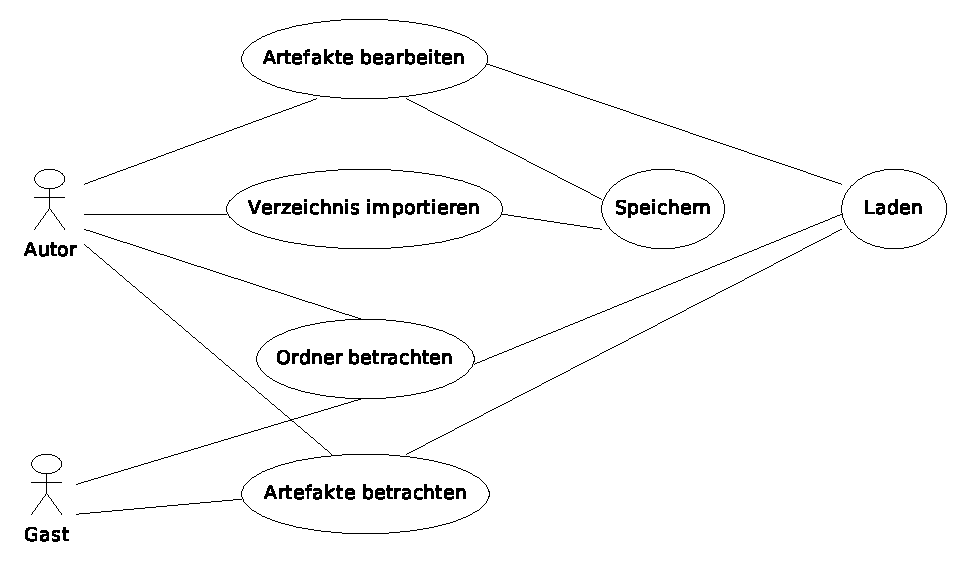
\includegraphics[width=15cm,keepaspectratio]{img/webbook_use_cases}
\caption{\code{webbook} Anwendungsf�lle}
\label{usecases}
\end{figure}

Zum besseren �berblick f�hren Anwendungsfalldiagramme auch Benutzergruppen ein.
Hier -- auf der linken Seite dargestellt -- werden die Rollen "Autor" und "Gast"
modelliert. Durch die Verbindungslinien werden die erlaubten Anwendungsf�lle
dargestellt. Strichlierte Pfeile stehen f�r Anwendungsfallinklusion. Zum
Beispiel muss f�r den Anwendungfall "Ordner betrachten" der Anwendungsfall
"Laden" abgearbeitet werden.

Ebenso wie bei der Datenbankmodellierung k�nnen die Objekte und Attribute des
fach\-spe\-zi\-fi\-schen Wissensmodelles in die Objekte des Datenmodelles �bernommen
werden. Da Objekte an sich bereits unterscheidbar sind, ben�tigen sie keine
besonderen Vorkehrungen f�r die Identifizierung. Diese Informationen sind erst
sp�ter f�r allf�llige Such- und Ablagesysteme von Bedeutung. Sachlogische
Zusammenh�nge werden daher auch ohne Umweg �ber Schl�sselwerte als Verweise auf
andere Objekte modelliert.

%% TODO: diesen cheat hier �berpr�fen (lstlisting kann nicht in pdf-verzeichnis genutzt werden)
\section{Die \emph{webbook} Beispieldatenbank}

Um die in dieser Diplomarbeit behandelten Methoden und Werkzeuge vergleichbar
zu machen, wurde eine kleine Bild- und Artikeldatenbank in Java implementiert.
Ziel war es, eine �berschaubare Schnittstelle unter Zuhilfenahme verschiedener
Bibliotheken und Werkzeuge umzusetzen, um Erfahrungen mit den Werkzeugen zu
sammeln und um daran die Effizienz und Effektivit�t beurteilen zu k�nnen.

Um die Funktionalit�t der Produkte zu demonstrieren implementiert die
Beispielanwendung lediglich den Datenzugriff und keine Benutzeroberfl�che. In
einer umfassenden Architektur k�nnte aufbauend auf den hier implementierten
Gesch�ftsobjekten die Gesch�ftslogik in einem Applikationsserver ablaufen.
Alternativ kann die Benutzeroberfl�che, zum Beispiel �ber einen Webserver,
direkt mit dieser Bibliothek arbeiten.

Die grundlegenden Objekte der Datenbank sind Artikel und Bilder. �ber
Schlagworte k�nnen Gruppen gebildet werden. Diese Objekte und ihre Attribute
werden im folgenden n�her beschrieben.

Der Java-Quelltext ist in der Eclipse Entwicklungsumgebung nach verwendeten
Werkzeugen in Projekte gegliedert; allen Implementierungen gemeinsam ist das
\code{Common} Projekt, in dem gemeinsame Schnittstellendefinitionen im Paket
\code{webbook} und die Modultests im Paket \code{webbook.tests} definiert sind.
Abbildung~\ref{ueberblick} zeigt das \code{Common} Projekt und die darin
enthaltenen Schnittstellen und Klassen.

\begin{figure}
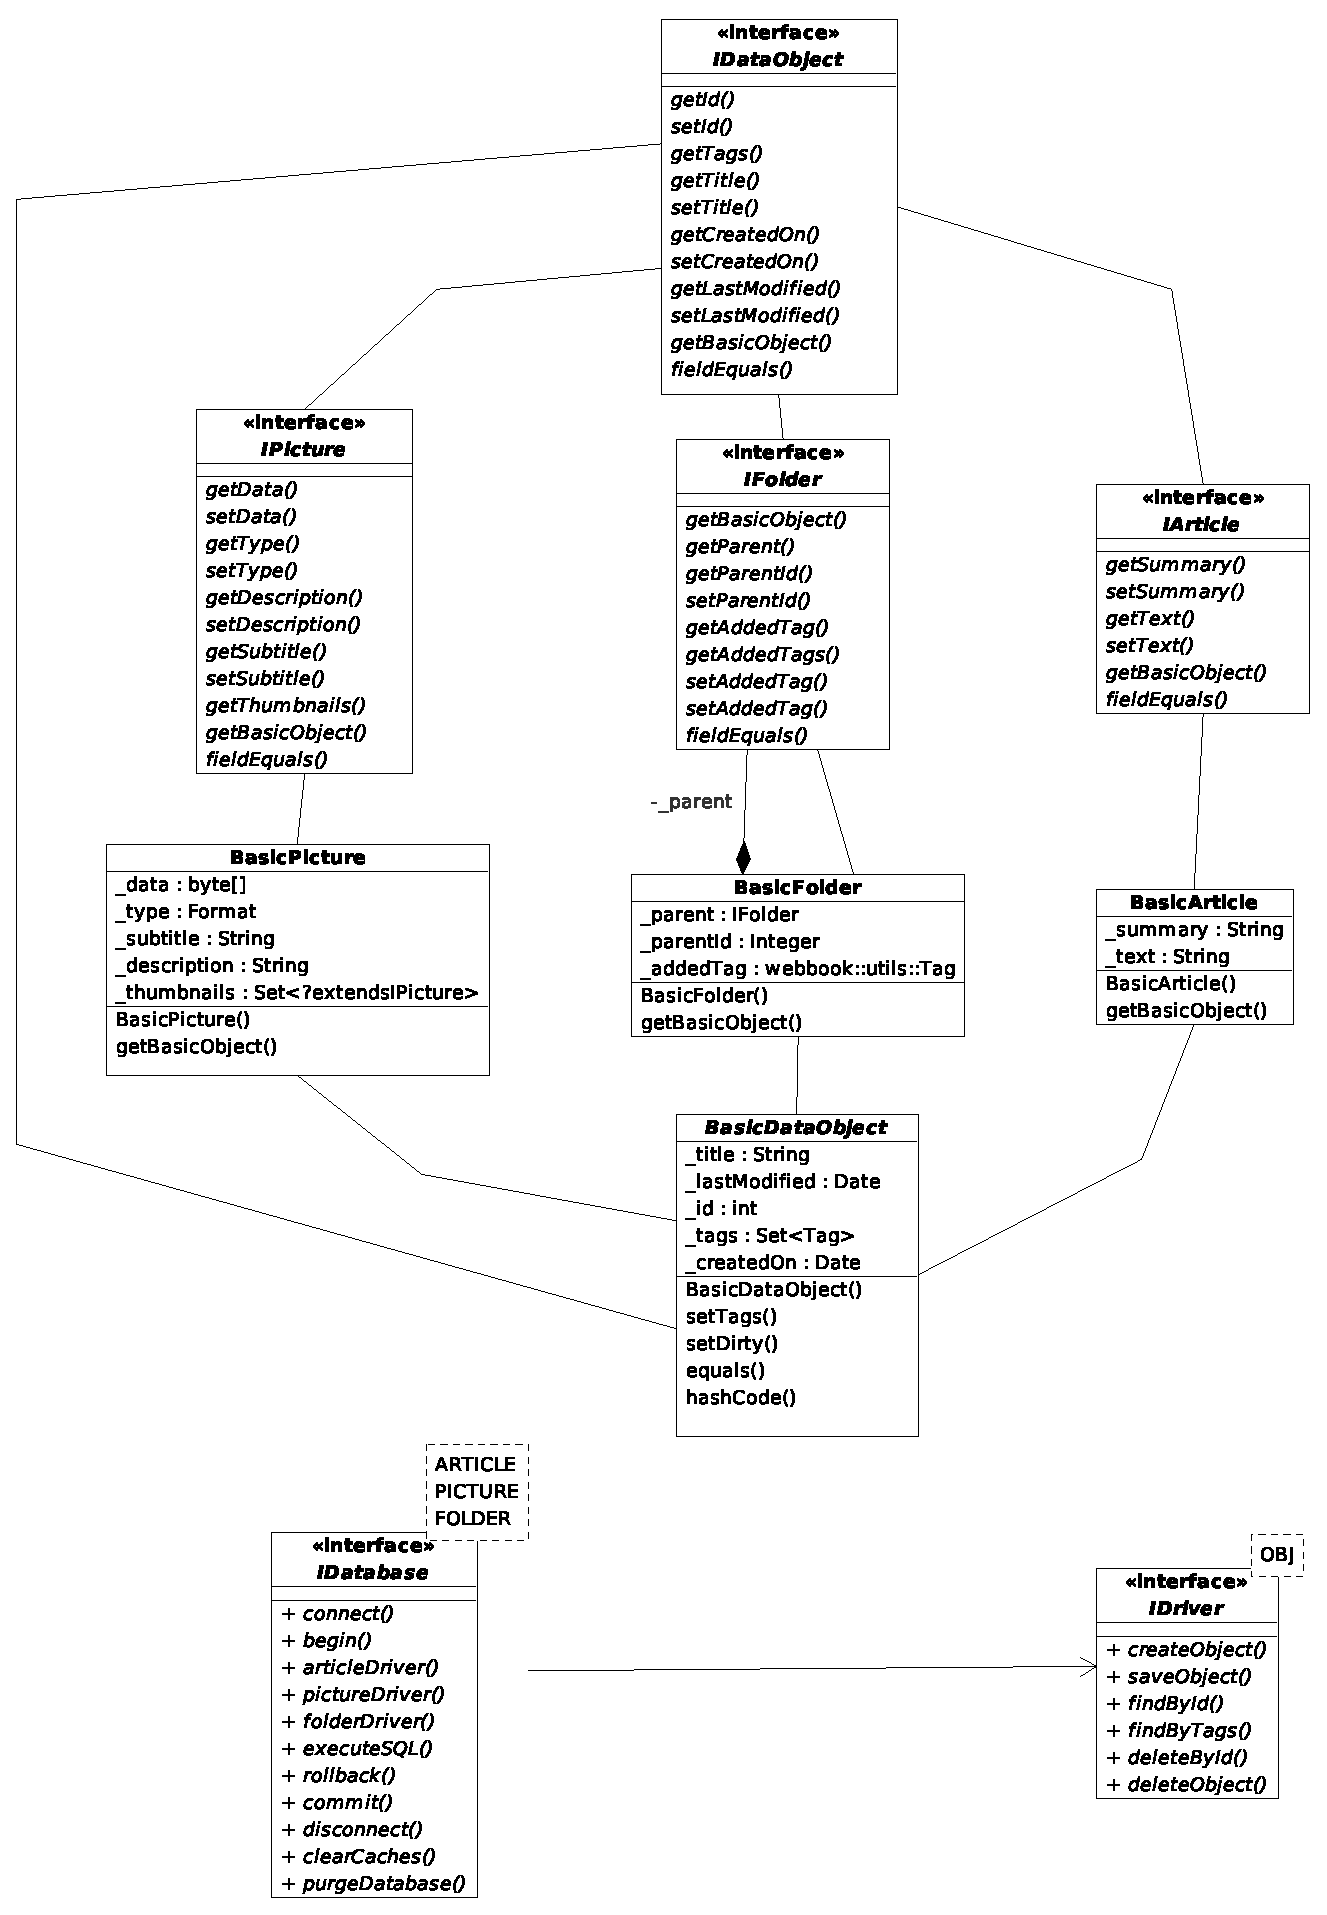
\includegraphics[width=15cm,keepaspectratio]{img/overview}
\caption{�berblick �ber die \code{webbook} Objekte}
\label{ueberblick}
\end{figure}

\subsection{Schnittstellen}

Das \code{IDataObject} ist das Kernst�ck des gesamten Modells und
Basisklasse f�r die anderen Objekte. Es enth�lt jene Attribute, die allen
Artefakten gemein sind: eine eindeutige ID, Er\-zeu\-gungs-
und Modifikationsdatum, einen Titel und die Menge von Schlagworten, die diesem
Objekt zugeordnet sind. Die Attribute sind als einfache \code{get}- und
\code{set}-Zugriffsmethoden nach der Java Beans Konvention (Siehe
\cite{beans101}, 8.3) implementiert:

\begin{lstlisting}[caption=\lstinline{IDataObject}]
public interface IDataObject {

    public abstract int      getId();
    public abstract void     setId(int id);

    public abstract Set<Tag> getTags();

    public abstract String   getTitle();
    public abstract void     setTitle(String title);

    /* ... */
\end{lstlisting}

\code{IArticle} und \code{IPicture} definieren die weiteren
Attribute der Gesch�ftsobjekte: Zusammenfassung und Text f�r Artikel sowie
Bilddaten, -unterschriften und Beschreibungstexte f�r Bilder.

\begin{lstlisting}[caption=Datenobjekt am Beispiel von \lstinline{IPicture}]
public interface IPicture extends IDataObject {

    public abstract byte[] getData();
    public abstract void   setData(byte[] data);

    public abstract Set<? extends IPicture> getThumbnails();

    /* ... */
\end{lstlisting}

\begin{note}
Eine Menge von Objekten kann in Java in einem \code{Set} gespeichert werden.
Seit Java 1.5 gibt es mit der \code{Set<? extends IPicture>} Notation eine neue
Syntax um "Menge von Objekten einer von \code{IPicture} abgeleiteten Klasse" zu
definieren. Typparameter f�r Klassen werden sp�ter besonders bei den Tests
verwendet.
\end{note}

Der \code{IFolder} ist eine M�glichkeit, aus der engen Folksonomie (siehe
\cite{folksonomy}, 3.2.3) der Schlagworte Gruppierungen zu bilden, die die enthaltenen
Strukturen abbilden. Sowohl die Mengenabfragen von Schlagw�rtern, als auch die
rekursiven Ordnerstrukturen sind von reinen relationalen Systemen nicht
befriedigend gel�st worden und sind daher interessante Beispiele um die Grenzen
von objekt-relationalen Abbildungen abzutasten.

\begin{lstlisting}[caption=Attribute von \lstinline{IFolder}]
public interface IFolder extends IDataObject {

    public abstract IFolder getParent();
    public abstract Tag getAddedTag();
    public abstract TagExpression getAddedTags();

    /* ... */
\end{lstlisting}

\begin{figure}
%%\includegraphics[width=15cm,keepaspectratio]{img/folder.pdf}
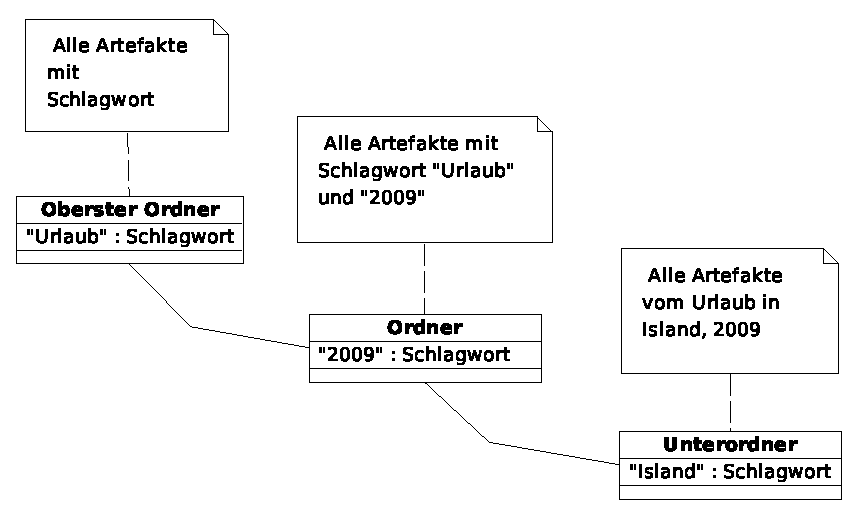
\includegraphics{img/folderstruct}
%%% Graphic for TeX using PGF
% Title: /home/david/Studium/Diplomarbeit/tex/img/Folder.dia
% Creator: Dia v0.95
% CreationDate: Sat Dec  9 18:10:54 2006
% For: david
% \usepackage{tikz}
% The following commands are not supported in PSTricks at present
% We define them conditionally, so when they are implemented,
% this pgf file will use them.
\ifx\du\undefined
  \newlength{\du}
\fi
\setlength{\du}{15\unitlength}
\begin{tikzpicture}
\pgftransformxscale{1.000000}
\pgftransformyscale{-1.000000}
\definecolor{dialinecolor}{rgb}{0.000000, 0.000000, 0.000000}
\pgfsetstrokecolor{dialinecolor}
\definecolor{dialinecolor}{rgb}{1.000000, 1.000000, 1.000000}
\pgfsetfillcolor{dialinecolor}
\pgfsetlinewidth{0.100000\du}
\pgfsetdash{}{0pt}
\pgfsetdash{}{0pt}
\pgfsetmiterjoin
{\pgfsetcornersarced{\pgfpoint{0.000000\du}{0.000000\du}}\definecolor{dialinecolor}{rgb}{0.000000, 0.000000, 0.000000}
\pgfsetstrokecolor{dialinecolor}
\draw (1.000000\du,5.000000\du)--(1.000000\du,6.800000\du)--(5.900000\du,6.800000\du)--(5.900000\du,5.000000\du)--cycle;
}% setfont left to latex
\definecolor{dialinecolor}{rgb}{0.000000, 0.000000, 0.000000}
\pgfsetstrokecolor{dialinecolor}
\node at (3.450000\du,5.975000\du){IFolder};
\pgfsetlinewidth{0.100000\du}
\pgfsetdash{}{0pt}
\pgfsetdash{}{0pt}
\pgfsetmiterjoin
{\pgfsetcornersarced{\pgfpoint{0.000000\du}{0.000000\du}}\definecolor{dialinecolor}{rgb}{0.000000, 0.000000, 0.000000}
\pgfsetstrokecolor{dialinecolor}
\draw (15.000000\du,13.000000\du)--(15.000000\du,14.800000\du)--(19.900000\du,14.800000\du)--(19.900000\du,13.000000\du)--cycle;
}% setfont left to latex
\definecolor{dialinecolor}{rgb}{0.000000, 0.000000, 0.000000}
\pgfsetstrokecolor{dialinecolor}
\node at (17.450000\du,13.975000\du){IFolder};
\pgfsetlinewidth{0.100000\du}
\pgfsetdash{}{0pt}
\pgfsetdash{}{0pt}
\pgfsetmiterjoin
{\pgfsetcornersarced{\pgfpoint{0.000000\du}{0.000000\du}}\definecolor{dialinecolor}{rgb}{0.000000, 0.000000, 0.000000}
\pgfsetstrokecolor{dialinecolor}
\draw (8.000000\du,9.000000\du)--(8.000000\du,10.800000\du)--(12.900000\du,10.800000\du)--(12.900000\du,9.000000\du)--cycle;
}% setfont left to latex
\definecolor{dialinecolor}{rgb}{0.000000, 0.000000, 0.000000}
\pgfsetstrokecolor{dialinecolor}
\node at (10.450000\du,9.975000\du){IFolder};
\pgfsetlinewidth{0.100000\du}
\pgfsetdash{}{0pt}
\pgfsetdash{}{0pt}
\pgfsetmiterjoin
\pgfsetbuttcap
{
\definecolor{dialinecolor}{rgb}{0.000000, 0.000000, 0.000000}
\pgfsetfillcolor{dialinecolor}
% was here!!!
\pgfsetarrowsend{stealth}
{\pgfsetcornersarced{\pgfpoint{0.000000\du}{0.000000\du}}\definecolor{dialinecolor}{rgb}{0.000000, 0.000000, 0.000000}
\pgfsetstrokecolor{dialinecolor}
\draw (3.450000\du,6.800000\du)--(8.000000\du,9.900000\du);
}}
\pgfsetlinewidth{0.100000\du}
\pgfsetdash{}{0pt}
\pgfsetdash{}{0pt}
\pgfsetmiterjoin
\pgfsetbuttcap
{
\definecolor{dialinecolor}{rgb}{0.000000, 0.000000, 0.000000}
\pgfsetfillcolor{dialinecolor}
% was here!!!
\pgfsetarrowsend{stealth}
{\pgfsetcornersarced{\pgfpoint{0.000000\du}{0.000000\du}}\definecolor{dialinecolor}{rgb}{0.000000, 0.000000, 0.000000}
\pgfsetstrokecolor{dialinecolor}
\draw (10.450000\du,10.800000\du)--(15.000000\du,13.900000\du);
}}
% setfont left to latex
\definecolor{dialinecolor}{rgb}{0.000000, 0.000000, 0.000000}
\pgfsetstrokecolor{dialinecolor}
\node[anchor=east] at (5.000000\du,9.000000\du){addedTag};
\definecolor{dialinecolor}{rgb}{0.000000, 0.000000, 0.000000}
\pgfsetstrokecolor{dialinecolor}
\node[anchor=east] at (5.000000\du,9.800000\du){= "Urlaub"};
% setfont left to latex
\definecolor{dialinecolor}{rgb}{0.000000, 0.000000, 0.000000}
\pgfsetstrokecolor{dialinecolor}
\node[anchor=east] at (12.000000\du,13.000000\du){addedTag};
\definecolor{dialinecolor}{rgb}{0.000000, 0.000000, 0.000000}
\pgfsetstrokecolor{dialinecolor}
\node[anchor=east] at (12.000000\du,13.800000\du){= "2006"};
\pgfsetlinewidth{0.100000\du}
\pgfsetdash{}{0pt}
\definecolor{dialinecolor}{rgb}{1.000000, 1.000000, 1.000000}
\pgfsetfillcolor{dialinecolor}
\fill (1.000000\du,1.000000\du)--(5.150000\du,1.000000\du)--(5.750000\du,1.600000\du)--(5.750000\du,2.700000\du)--(1.000000\du,2.700000\du)--cycle;
\definecolor{dialinecolor}{rgb}{0.000000, 0.000000, 0.000000}
\pgfsetstrokecolor{dialinecolor}
\draw (1.000000\du,1.000000\du)--(5.150000\du,1.000000\du)--(5.750000\du,1.600000\du)--(5.750000\du,2.700000\du)--(1.000000\du,2.700000\du)--cycle;
\pgfsetlinewidth{0.050000\du}
\definecolor{dialinecolor}{rgb}{0.000000, 0.000000, 0.000000}
\pgfsetstrokecolor{dialinecolor}
\draw (5.150000\du,1.000000\du)--(5.150000\du,1.600000\du)--(5.750000\du,1.600000\du);
% setfont left to latex
\definecolor{dialinecolor}{rgb}{0.000000, 0.000000, 0.000000}
\pgfsetstrokecolor{dialinecolor}
\node[anchor=west] at (1.350000\du,2.200000\du){alle Bilder};
\pgfsetlinewidth{0.100000\du}
\pgfsetdash{}{0pt}
\definecolor{dialinecolor}{rgb}{1.000000, 1.000000, 1.000000}
\pgfsetfillcolor{dialinecolor}
\fill (7.000000\du,3.000000\du)--(13.600000\du,3.000000\du)--(14.200000\du,3.600000\du)--(14.200000\du,4.700000\du)--(7.000000\du,4.700000\du)--cycle;
\definecolor{dialinecolor}{rgb}{0.000000, 0.000000, 0.000000}
\pgfsetstrokecolor{dialinecolor}
\draw (7.000000\du,3.000000\du)--(13.600000\du,3.000000\du)--(14.200000\du,3.600000\du)--(14.200000\du,4.700000\du)--(7.000000\du,4.700000\du)--cycle;
\pgfsetlinewidth{0.050000\du}
\definecolor{dialinecolor}{rgb}{0.000000, 0.000000, 0.000000}
\pgfsetstrokecolor{dialinecolor}
\draw (13.600000\du,3.000000\du)--(13.600000\du,3.600000\du)--(14.200000\du,3.600000\du);
% setfont left to latex
\definecolor{dialinecolor}{rgb}{0.000000, 0.000000, 0.000000}
\pgfsetstrokecolor{dialinecolor}
\node[anchor=west] at (7.350000\du,4.200000\du){alle Urlaubsbilder};
\pgfsetlinewidth{0.100000\du}
\pgfsetdash{}{0pt}
\definecolor{dialinecolor}{rgb}{1.000000, 1.000000, 1.000000}
\pgfsetfillcolor{dialinecolor}
\fill (14.000000\du,6.000000\du)--(20.600000\du,6.000000\du)--(21.200000\du,6.600000\du)--(21.200000\du,8.500000\du)--(14.000000\du,8.500000\du)--cycle;
\definecolor{dialinecolor}{rgb}{0.000000, 0.000000, 0.000000}
\pgfsetstrokecolor{dialinecolor}
\draw (14.000000\du,6.000000\du)--(20.600000\du,6.000000\du)--(21.200000\du,6.600000\du)--(21.200000\du,8.500000\du)--(14.000000\du,8.500000\du)--cycle;
\pgfsetlinewidth{0.050000\du}
\definecolor{dialinecolor}{rgb}{0.000000, 0.000000, 0.000000}
\pgfsetstrokecolor{dialinecolor}
\draw (20.600000\du,6.000000\du)--(20.600000\du,6.600000\du)--(21.200000\du,6.600000\du);
% setfont left to latex
\definecolor{dialinecolor}{rgb}{0.000000, 0.000000, 0.000000}
\pgfsetstrokecolor{dialinecolor}
\node[anchor=west] at (14.350000\du,7.200000\du){alle Urlaubsbilder};
\definecolor{dialinecolor}{rgb}{0.000000, 0.000000, 0.000000}
\pgfsetstrokecolor{dialinecolor}
\node[anchor=west] at (14.350000\du,8.000000\du){aus 2006};
\pgfsetlinewidth{0.100000\du}
\pgfsetdash{{\pgflinewidth}{0.200000\du}}{0cm}
\pgfsetdash{{\pgflinewidth}{0.200000\du}}{0cm}
\pgfsetbuttcap
{
\definecolor{dialinecolor}{rgb}{0.000000, 0.000000, 0.000000}
\pgfsetfillcolor{dialinecolor}
% was here!!!
\definecolor{dialinecolor}{rgb}{0.000000, 0.000000, 0.000000}
\pgfsetstrokecolor{dialinecolor}
\draw (3.375000\du,2.700000\du)--(3.450000\du,5.000000\du);
}
\pgfsetlinewidth{0.100000\du}
\pgfsetdash{{\pgflinewidth}{0.200000\du}}{0cm}
\pgfsetdash{{\pgflinewidth}{0.200000\du}}{0cm}
\pgfsetbuttcap
{
\definecolor{dialinecolor}{rgb}{0.000000, 0.000000, 0.000000}
\pgfsetfillcolor{dialinecolor}
% was here!!!
\definecolor{dialinecolor}{rgb}{0.000000, 0.000000, 0.000000}
\pgfsetstrokecolor{dialinecolor}
\draw (10.600000\du,4.700000\du)--(10.450000\du,9.000000\du);
}
\pgfsetlinewidth{0.100000\du}
\pgfsetdash{{\pgflinewidth}{0.200000\du}}{0cm}
\pgfsetdash{{\pgflinewidth}{0.200000\du}}{0cm}
\pgfsetbuttcap
{
\definecolor{dialinecolor}{rgb}{0.000000, 0.000000, 0.000000}
\pgfsetfillcolor{dialinecolor}
% was here!!!
\definecolor{dialinecolor}{rgb}{0.000000, 0.000000, 0.000000}
\pgfsetstrokecolor{dialinecolor}
\draw (17.600000\du,8.500000\du)--(17.450000\du,13.000000\du);
}
\end{tikzpicture}

\caption{Folderstruktur}
\label{folderstruktur}
\end{figure}

Die \code{IDatabase} Schnittstelle enth�lt alle Datenbank-relevanten
Operationen f�r die Ver\-bin\-dungs- und Transaktionsverwaltung, sowie Methoden zum
Laden und Speichern der Artefakte.

Alle Schnittstellen in diesem Projekt sind mit generischen Typparametern
versehen. So haben alle konkreten Implementierungen die gleiche Aussenform und
arbeiten doch mit ihren eigenen, konkreten Typen.

\section{Datensicherheit}

Um in einem Programmiersystem Daten sinnvoll verwalten zu k�nnen, muss das
System zumindest die folgenden vier Anforderungen erf�llen:\label{ACID}

\begin{description}
\item[Atomare Transaktion:]{Eine Transaktion heisst atomar, wenn alle Anweisungen
aus denen die Transaktion besteht ganz oder gar nicht durchgef�hrt werden.
Dazu wird zu Beginn der Ausf�hrung ein Eintrag in eine Logdatei geschrieben.
Alle �nderungen an der Datenbank versieht das DBMS mit einem Verweis auf den
zugeh�rigen Eintrag in dieser Logdatei. Wurde die Anweisung erfolgreich
abgeschlossen, wird dies in der Logdatei ebenfalls verzeichnet. Ist es notwendig
den Zustand der Datenbank nach einem Absturz zu rekonstruieren, k�nnen anhand
der Logdatei die offenen Transaktion aufgefunden und die potentiell fehlerhaften
oder nur teilweise durchgef�hrten Anweisungen aufger�umt werden.}
\item[Konsistenz:]{Um die Qualit�t des Datenbestandes jederzeit zu
gew�hrleisten, muss ein DBMS daf�r Sorge tragen, dass die angegebene
Randbedingungen (Datentypen, Wertebereiche, gegenseitige Abh�ngigkeiten) f�r die
Daten zu jedem Zeitpunkt eingehalten werden. Dazu werden diese Randbedingungen
sp�testens beim Abschluss einer Transaktion �berpr�ft. Wird dabei eine
potentielle Inkonsistenz entdeckt, bricht die Operation ab und die bisher
get�tigten
�nderungen werden r�ckg�ngig gemacht.}
\item[Isolierung:]{Die Forderung nach Korrektheit im Mehrbenutzerbetrieb erweitert die
Kon\-sis\-tenz\-an\-for\-der\-ungen um einen wichtigen Aspekt: parallel ablaufende
Anweisungen d�rfen sich nicht gegenseitig st�ren. Das formale Kriterium hierf�r
-- die Serialisierbarkeit der Abl�ufe --
lautet, dass sich die Datenbank so verh�lt, als ob alle Anweisungen nacheinander
statt gleichzeitig ausgef�hrt werden. Bei einzelnen Anweisungen ist das durch
triviale Zeilen- oder Tabellensperren implementierbar. Isolierung �ber mehrere
Anweisungen hinweg wird sp�ter im folgenden Abschnitt~\ref{transactions}~Transaktionen
noch detaillierter besprochen.}
\item[Dauerhaftigkeit:]{Meldet ein DBMS die erfolgreiche Durchf�hrung einer
Transaktion, so muss diese -- im Rahmen der physikalischen M�glichkeiten -- auch
gesichert und dauerhaft gespeichert sein.}
\end{description}

Die daf�r oft verwendete Abk�rzung lautet "ACID", aus dem Englischen von
Atomicity, Consistency, Isolation und Durability -- Atomare Operationen,
Konsistenz, Isolierung und Dauerhaftigkeit.

\TODO{Literatur!}

\section{Transaktionen}
\label{transactions}

Um komplexere Operationen durchzuf�hren, kann man einzelne Basisoperationen
in einer Transaktion zusammenfassen. Die Transaktion als Ganzes erf�llt dann
wieder die ACID Anforderungen. Konsistenz und Dauerhaftigkeit folgen aus den
entsprechenden Kriterien f�r Einzelanweisungen transitiv: Wenn jede einzelne
Anweisung korrekt ist und die Ergebnisse dauerhaft gespeichert werden, dann
m�ssen auch Aneinanderreihungen solcher Anweisung korrekt und dauerhaft sein.

Das Kriterium der Serialisierung -- die virtuelle Nacheinanderausf�hrung von
Anweisungen -- gilt selbstverst�ndlich ebenfalls f�r Transaktionen. W�hrend selbst
bei komplexen Einzelanweisungen eine Isolierung zwischen gleichzeitig laufenden
Anweisungen mittels Sperren einfach ist, f�hrt ein unbedachter Einsatz von
Sperren in l�nger laufenden Transaktionen zu gravierenden
Leistungsverlusten, da die meisten Benutzer darauf warten m�ssen, dass
die gerade laufende, fremde Transaktion abgeschlossen wird.

Auf der Anwendungsseite kann dem durch die Vermeidung von lang laufenden
Transaktionen entgegengewirkt werden.

\TODO{forward-referenz auf Behandlung lang laufender Transaktionen}

Um Transaktionen atomar zu halten, m�ssen entweder alle oder keine der
Anweisungen durchgef�hrt werden. Das klassische Beispiel dazu ist eine
�berweisung von einem Konto auf ein anderes Konto. Um eine solche �berweisung
durchzuf�hren, wird vom Ursprungskonto der Betrag abgezogen, w�hrend am
Zielkonto der Betrag hinzuaddiert wird. W�rde aufgrund einer Fehlersituation zum
Beispiel nur der Betrag abgebucht aber nicht wieder gutgeschrieben, so
verschw�nde der Betrag spurlos im Nichts.

Ein anderes Problem von Transaktionen ist die M�glichkeit zum sogenannten
\emph{Deadlock}. Dabei warten zwei Transaktionen jeweils auf die von der anderen
Transaktion gesperrten Ressourcen. Da keine der beiden Transaktionen fortfahren
kann bevor die andere nicht ihre Resourcen freigibt, bleiben sie -- ohne
Eingriff von aussen -- ewig stecken. Die Methoden um solche Probleme zu
entdecken und zu behandeln sind nicht Inhalt dieser Diplomarbeit.

\TODO{Literatur!}

\section{Basisoperationen}

Die Minimalanforderungen f�r die Datenverwaltung sind im Akronym
"CRUD", vom englischen Create, Read, Update und Delete, zusammengefasst. Auf
Deutsch: Datenobjekte m�ssen erzeugt, gelesen, ver�ndert und gel�scht werden
k�nnen.

\TODO{Literatur!}

In SQL werden die Basisoperationen mit diesen Befehlen durchgef�hrt:

\begin{lstlisting}[language=SQL, caption=Grundlegende SQL Befehle]
-- Erzeugen einer Datenzeile
INSERT INTO tabelle (attr1, attr2) VALUES (wert1, wert2);

-- Abrufen
SELECT attr1, attr2 FROM tabelle WHERE bedingung;

-- �ndern
UPDATE tabelle SET attr1 = wert1 WHERE bedingung;

-- L�schen
DELETE FROM tabelle WHERE bedingung;
\end{lstlisting}

Dabei ist vor allem zu beachten, dass -- bis auf \code{INSERT} -- immer auf
Mengen von Da\-ten\-zei\-len operiert wird, die die pr�dikatenlogische Formel
\code{bedingung} erf�llen. Diese Mengen k�nnen nat�rlich auch kein oder nur ein
Element enthalten.

In Java hingegen sind die Basisoperationen zwischen dem
\lstinline{IDatabase} Interface und den einzelnen Klassen aufgeteilt.

\begin{lstlisting}[caption=\lstinline{IDatabase} Operationen]
/* Erzeugen */
public abstract OBJ createObject();

/* Abrufen */
public abstract OBJ findById(int id) throws SQLException;
public abstract Set<? extends OBJ> findByTags(TagExpression tags) throws SQLException;

/* Abspeichern */
public abstract OBJ saveObject(OBJ o) throws SQLException;

/* L�schen */
public abstract OBJ deleteObject(OBJ o) throws SQLException;
\end{lstlisting}

�nderungen an Objekten werden direkt an den Objekten vorgenommen und �ber die
\lstinline{IDatabase} Schnittstelle als Ganzes gespeichert. Es bleibt dem Framework
�berlassen zu entscheiden wie die Daten gespeichert werden sollen. Im Gegensatz
zu SQL sieht man sofort, dass die Abfragen wesentlich eingeschr�nkter sind,
daf�r aber auf einer wesentlich h�heren Ebene formuliert werden.

\section{Programmierung}

Ein fundamentales Problem der Programmierung objekt-relationaler Anwendungen ist
die Notwendigkeit, Programmtext und Datenbankschema synchron zu halten. Selbst im
einfachsten Fall existieren f�nf Listen aller Attribute eines Objektes: bei der
Datenbank- und Objektdefinition sowie in den Datenbankanweisungen f�r Create,
Read und Update, da hier ja immer Attributswerte von und zur Datenbank kopiert
werden m�ssen. Bei diesen Kopiervorg�ngen bringen objekt-relationale
Abbildungen eine erh�hte Sicherheit, da sie durch die Werkzeuge weitestgehend
automatisiert werden.

\subsection{Datentypen}

Mit geringerem Aufwand aber h�herer Komplexit�t ist die Konversion
zwischen programmiersprachlichen Datentypen und jenen der Datenbank zu beachten.
\begin{description}
\item[Zahlentypen:]{Da sich Wertebereiche und Genauigkeit oft an den
M�glichkeiten der zugrunde liegenden Hardware und damit an weitverbreiteten
Standards (zum Beispiel \cite{ieee754} f�r Gleitkommazahlen) orientieren, kann
bei diesen Datentypen oft eine eindeutige Zuordnung getroffen werden.}
\item[Zeichenketten:]{W�hrend bei Programmiersprachen Zeichenketten unbeschr�nkt
sind, enthalten Datenbanken oft starke Optimierungen f�r l�ngenbeschr�nkte
Zeichenketten. Das Objektmodell muss die Einschr�nkungen des Datenbankschemas
erzwingen, um Lauf\-zeit- und Konsistenzfehler zu vermeiden. Versch�rft werden
diese Probleme noch durch eventuell erforderliche Zeichensatzkonversionen
zwischen verschiedenen Anwendungsteilen und Zeichenkodierungen wie UTF-8, die einen
variablem Platzbedarf bei konstanter Zeichenanzahl haben.}
\item[Zeit- und Datumsangaben:]{Wertebereich, Genauigkeit, Epoche, interne
Repr�sentation (Fixkomma oder Gleitkomma), externe Repr�sentation
(US-amerikanisch, europ�isch, international), Zeitzonen, Kalender, Schalttage, 
-minuten und -sekunden, unterschiedliche Zeitquellen, Fehlerbehandlung.
Subtile und nicht so subtile Unterschiede in diesen Parametern f�hren --
zusammen mit komplexen und daher mangelhaft implementierten Standards --
unweigerlich zu Problemen in der Kommunikation zwischen verschiedenen Produkten.
Einige Probleme k�nnen durch eine gemeinsame, anwendungsweite, externe
Repr�sentation, die ohne Genauigkeitsverlust in alle beteiligten internen
Repr�sentation ein-eindeutig umgewandelt werden kann, behoben werden. Dadurch
k�nnen Werte -- die Korrektheit der Umwandlungen vorausgesetzt -- beliebig oft
umgewandelt werden ohne die gespeicherten Zeitpunkte zu verwischen.

Andere Probleme -- zum Beispiel wie sich Systeme in den Umschaltstunden zum
Sommerzeitwechsel zu verhalten haben -- k�nnen nur durch eine pr�zise Definition
des gew�nschten Verhaltens umgangen werden. }
\item[Boolsche Werte:]{Die Unterst�zung von Bit-Werten schwankt zwischen
verschiedenen Datenbanksystemen stark. Eine portable Alternative bildet
Wahrheitswerte auf die Zeichen 'w' und 'f' -- f�r wahr und falsch -- ab und
sorgt mittels Konsistenzbedingungen f�r die Einhaltung dieser Konvention.}
\end{description}

Um umfangreichere Datenmengen -- zum Beispiel Bilddateien oder unbeschr�nkte
Texte -- direkt in der Datenbank zu verwalten werden sogenannte BLOBs oder
CLOBs\footnote{Binary Large OBjects und Character Large OBjects, f�r gro�e
Bin�r- oder Textmengen.} zur Verf�gung gestellt. Um das Laufzeit-, Speicher- und
Kommunikationsverhalten dieser Daten im Griff zu behalten, werden daf�r meist
zeichenstromorientierte Schnittstellen zur Verf�gung gestellt, die wiederum
seperat bedient werden m�ssen. Unterst�tzung f�r diese Datentypen ist
weitverbreitet.

Neben diesen Standardtypen gilt es, f�r eine Vielzahl von komplexeren Datentypen
effiziente Abbildungen und Konversionen zu finden. Um nur einige Beispiele zu
nennen: Netzwerkadressen oder geometrische Daten f�r Geoinformationssysteme. Da
es sich dabei um kaum oder gar nicht standardisierte Erweiterungen handelt, ist
auch selten Unterst�tzung in Programmierwerkzeugen daf�r vorhanden. 

\subsection{Abfragen}

Abfragen auf einer Datenbank k�nnen um Gr��enordnungen schneller sein als
gleichwertige Abfragen auf dem Objektmodell. Drei grundlegende Ursachen k�nnen
dabei festgestellt werden:

\begin{description}
\item[Optimierung:] Die Abfrageoptimierung ist ein intensiv erforschtes Gebiet
der Datenbankprogrammierung. Sowohl auf der Seite der Programmierer als auch auf
Seite der Datenbanken selbst existieren Rezepte um die bekannten Flaschenh�lse
zu umgehen.
\item[Kommunikations- und Transformationsaufwand:] Wird die Datenbank direkt
abgefragt, so mu� nur das gew�nschte Abfrageergebnis zum Benutzer �bertragen
werden. Wird die gleiche Abfrage jedoch �ber ein zwischengeschaltetes
Objektmodell moderiert, m�ssen potentiell alle Daten aller beteiligten Objete
�bertragen und interpretiert werden, auch wenn diese f�r die Berechnung
irrelevant sind.
\item[Abfragekomplexit�t:] Abfragen die im Objektmodell sehr einfach zu
formulieren sind, k�nnen bei der Ausf�hrung auf der Datenbank nur schwer
umsetzbar sein. Speziell polymorphe Abfragen und Abfragen nach komplexen
berechneten Werden -- zum Beispiel "Kreditw�rdigkeit" -- werden in
objekt-orientierten Systemen direkt unterst�tzt, w�hrend sie in relationalen
Systemen aufw�ndig nachprogrammiert werden m�ssen.
\end{description}

\subsection{Portabilit�t}

Um die Abh�ngigkeit von einem Datenbankhersteller zu minimieren ist die
Portabilit�t zwischen unterschiedlichen Herstellern auch eine wichtige
Anforderung an eine objekt-relationale Abbildung. Um diese Unabh�ngigkeit zu
erreichen, werden die programmierten Abfragen in datenbankspezifische
Anweisungen �bersetzt.

\section{Kommunikation}

Sobald eine Anwendung aus mehr als einem (System-)Prozess besteht, wird die
Kommunikation zwischen diesen Prozessen zu einem Kernproblem der gesamten
Anwendung.

\paragraph{Zur Erh�hung des Transaktionsdurchsatzes} werden mehrere,
gleichzeitig arbeitende Systemprozesse eingesetzt. Um dabei die Korrektheit der
Daten zu garantieren,
m�ssen dabei auch die Anforderungen von CRUD und ACID �ber alle Prozesse hinweg
erf�llt werden. Da diese bereits von allen �blichen Datenbankimplementierungen
abgedeckt werden, bietet sich ein zentraler Datenbankserver an, als Angelpunkt
f�r eine Mehrprozessarchitektur zu dienen.

\begin{samepage}
\paragraph{Zur Einbettung in Dritt-Anwendungen} m�ssen
Kommunikationsschnittstellen nach au�en zur Verf�gung gestellt werden. Eine
interessante Entwicklung in diesem Bereich ist die serviceorientierte
Architektur (SOA). Hier werden Daten und Funktionalit�t �ber
herstellerunabh�ngige Protokolle und Formate (zum Beispiel HTTP,
SOAP und XML) im Netzwerk angeboten.
Eine detaillierte Behandlung w�rde jedoch den Rahmen dieser Arbeit
bei Weitem sprengen.
\end{samepage}


\chapter{Konzepte}
\thispagestyle{empty}
\label{Kapitel_Konzepte}

In der h�ndischen Modellierung wird, ausgehend von dem fachspezifischen
Wissensmodell, die technischen Modelle f�r Relationen und Objekte abgeleitet.
Dabei m�ssen
die beiden Modelle bez�glich Attributen und Wertebereichen aufeinander
abgestimmt sein. Abbildung~\ref{klassisch} illustriert diesen Vorgang. 

\begin{figure}
\hfill
\begin{minipage}[t]{.45\textwidth}
\begin{center}
%%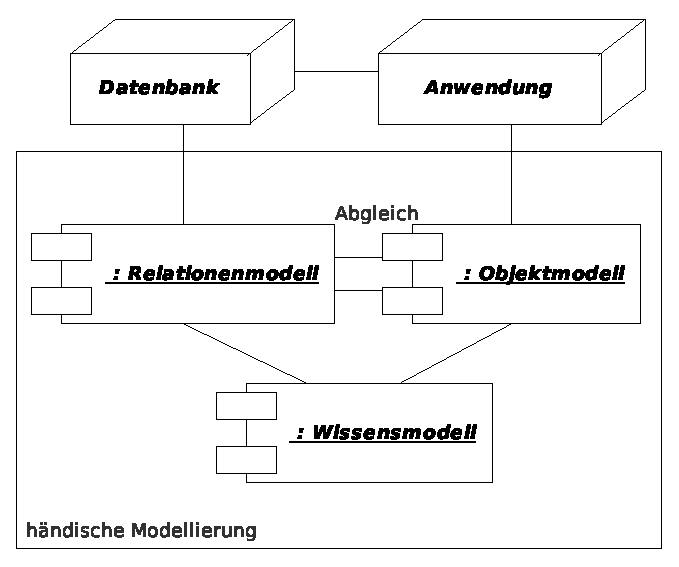
\includegraphics[width=15cm,keepaspectratio]{img/klassisch}
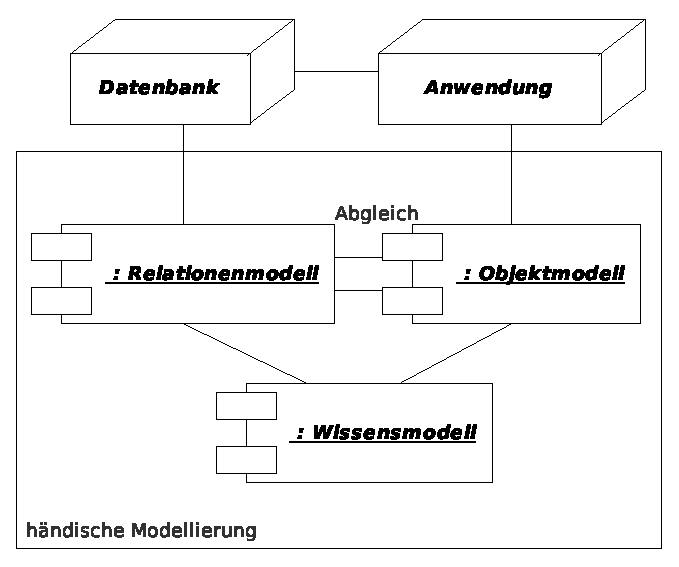
\includegraphics[width=.99\textwidth,keepaspectratio]{img/klassisch}
\end{center}
\caption{Klassische Architektur}
\label{klassisch}
\end{minipage}
\hfill
\begin{minipage}[t]{.45\textwidth}
\begin{center}
\includegraphics[width=.99\textwidth,keepaspectratio]{img/orm}
\end{center}
\caption{Architektur mit objekt-relationaler Abbildung}
\label{orm}
\end{minipage}
\hfill
\end{figure}

Bei dieser getrennten Behandlung der beiden technischen Modelle kommt es jedoch
zu Redundanzen zwischen diesen Modellen, die -- besonders bei �nderungen am
fachspezifischen Wissensmodell
-- zu unangenehmen Fehlerquellen werden. Hier setzt eine Implementierung mittels
objekt-relationaler Abbildung an, um die technische Modellierung zu
konzentrieren. Abbildung~\ref{orm} zeigt diese Alternative. Da durch die
Abbildung das Relationenmodell aus dem Objektmodell erzeugt werden kann, bleibt
auch bei �nderungen die interne Konsistenz erhalten.

F�r die Aufteilung der einzelnen Komponenten des Abbildungsapparates gibt es
verschiedene M�glichkeiten. Je nach Anforderungen des Projektes und der
Strukturierung der Entwicklung kann die Datenzugriffsschicht entweder direkt in
die Datenklassen \emph{integriert} oder f�r eine reduzierte Koppelung
\emph{getrennt} entwickelt werden. Zur Steigerung der Laufzeiteffizienz 
kann die Datenschicht w�hrend der Entwicklung erzeugt und
\emph{kompiliert} werden. Alternativ dazu kann eine erh�hte Flexibilit�t
gewonnen werden, indem die Datenschicht zur Laufzeit \emph{dynamisch
konfiguriert} wird.

\section{Funktionsumfang}

\TODO{in's Kapitel 5 verschieben?}

Das Ideal des praktischen Programmierers in Sachen objekt-orientierter
Persistenz w�re ein System mit der Einfachheit einer Datenbank und der
Ausdruckskraft einer modernen Programmiersprache. Ein solches System m�sste
atomare Transaktionen und Isolation zwischen Prozessen und Benutzern bieten,
sowie den vollen Funktionsumfang einer Programmiersprache. Au�erdem braucht so ein
System -- unabh�ngig von der Programmierung des Systems -- M�glichkeiten, um
�nderungen am physikalischen Schema zur Leistungsoptimierung durchzuf�hren.

Die folgenden Abschnitte besprechen M�glichkeiten, wie mit heute verf�gbaren
Mitteln solche Systeme gestaltet werden k�nnen. 

\TODO{Graphik um verschiedene Produkte(!) in diesem Koordinatensystem zu zeigen}
\TODO{hier kann noch �ber logische Unabh�ngigkeit gesprochen werden}

\section{Integrierte Datenschicht}

Mit einer \emph{integrierten Datenschicht} wird der Datenbankzugriff fest in die
Gesch�ftsobjekte eingebunden. Persistenzfunktionalit�t wird damit direkt in die
Objekthierarchie integriert. Diese Vorgehensweise maximiert die Koh�renz
zwischen Quelltext und Schema, da das Schema unmittelbar aus den im Quelltext
definierten Strukturen generiert wird. Abbildung~\ref{integriert} illustriert
diese Architektur.

\begin{figure}
\begin{center}
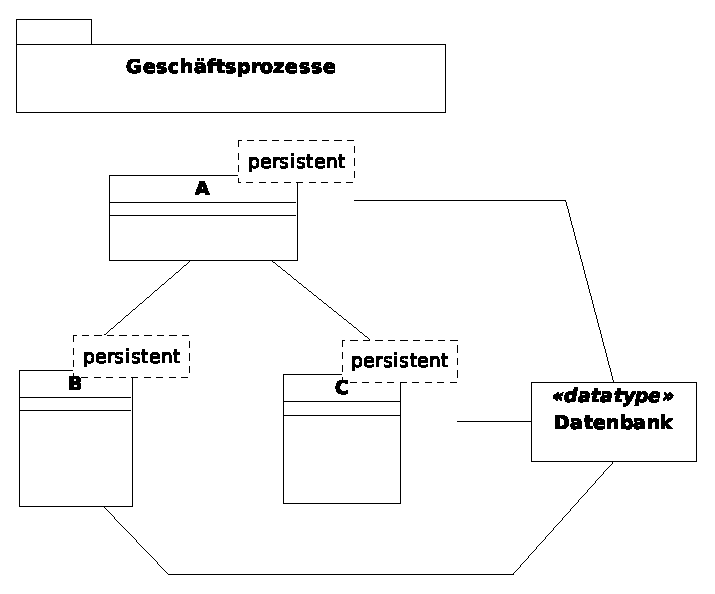
\includegraphics{img/integrierteDatenschicht}
\end{center}
\caption{Integrierte Datenschicht}
\label{integriert}
\end{figure}

Aufgrund der hohen Koppelung zwischen Anwendung und Datenschicht kann auf
ge\-ne\-ra\-li\-sie\-ren\-de Schnittstellen verzichtet werden. Die Anwendung kann
daher die Besonderheiten der verwendeten Datenschicht effizient nutzen. Wird die
Datenschicht im gleichen Projekt implementiert, kann auch besonders auf die
Anforderungen der Anwendung eingegangen werden. Durch die parallele Entwicklung
bedarf es -- jenseits der eigentlichen Programmierzeit -- keiner weiteren
Einarbeitung. Bei sehr kleinen Projekten kann das eine signifikante Ersparnis
sein.

Auf der anderen Seite schl�gt sich -- ebenfalls aufgrund der hohen Koppelung --
jede �nderung an der Datenschicht unmittelbar auf alle betroffenen Teile der
Anwendung durch. Insbesondere ist ein Ersetzen der Datenschicht durch eine
andere Implementierung mit hohem Aufwand verbunden.

\section{Getrennte Datenschicht}

\begin{figure}
\begin{center}
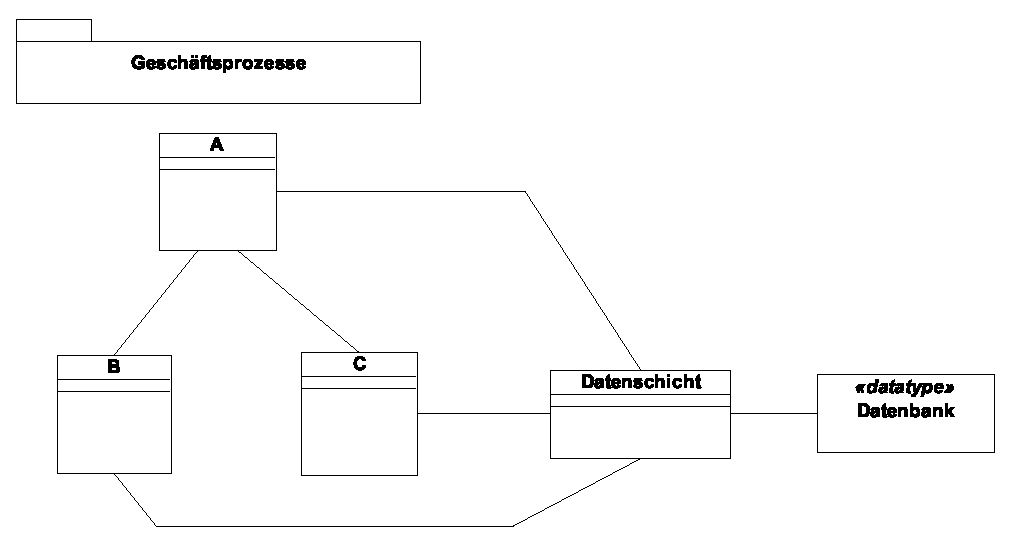
\includegraphics[width=.99\textwidth,keepaspectratio]{img/externeDatenschicht}
\end{center}
\caption{Getrennte Datenschicht}
\label{extern}
\end{figure}

Je gr��er Anwendungen werden, desto st�rker wird auch der Druck, einzelne
Komponenten an Spezialisten (innerhalb wie au�erhalb des Projektes) auszulagern. Da
gerade Datenbankagenden bereits zu einem hohen Ma� von Spezialisten bedient
werden, ist die Datenschicht ein guter Kandidat f�r eine architekturelle
Teilung. Abbildung~\ref{extern} illustriert die Anordnung der Komponenten.
Besonders zu beachten ist, dass die Gesch�ftsprozesse nun nichts mehr von der
internen Mechanik der Datenschicht wissen m�ssen.

Aufgrund dieser reduzierten Koppelung kann die Datenschicht auch ohne �nderung
der Gesch�ftsprozesse getauscht werden. Lediglich jene Teile der Gesch�ftslogik,
die Daten abfragen, sind nun von solchen �nderungen betroffen. Durch eine
passende \emph{Fassadenschnittstelle} zur Datenschicht kann auch die
Gesch�ftslogik von �nderungen dort gesch�tzt werden. Diese Fassade bietet auch
eine Plattform, um aus den daten-nahen Aufrufen der Datenschicht
gesch�fts-orientierte Methoden zu bauen.

\section{Implementierung der Datenschicht}

Unabh�ngig von der Beziehung der Datenschicht zu den Gesch�ftsobjekten, wird die
Art der Implementierung der Datenschicht gew�hlt. Grunds�tzlich besteht hier
kein Zusammenhang. In der Regel werden jedoch integrierte Datenschichten eher
statisch implementiert, w�hrend externe Datenschichten dynamische Methoden
bevorzugen, da diese eine weitere Reduzierung der Koppelung versprechen. 

\subsection{Statische Implementierung}

Vor allem bei der h�ndischen Implementierung einer Datenschicht in kleineren
Projekten kann sie \emph{direkt} in den Klassen der Gesch�ftsobjekte
implementiert werden. Dies stellt auch die st�rkste Form der oben besprochenen
integrierten Datenschicht dar: die Gesch�ftslogik manipuliert die Datenbank
unmittelbar.

Eine andere M�glichkeit der statischen Implementierung der Datenschicht ist die
\emph{automatisierte Quelltexterzeugung}. Aus einer externen Beschreibung des
Schemas werden Basisklassen erzeugt, die die reine Datenbankmanipulation
implementieren. Um die Gesch�ftslogik unabh�ngig vom Datenschema und dem
Erzeugungsprozess zu halten, wird sie in abgeleiteten Klassen implementiert.
Dadurch erh�lt sie Zugriff auf die erzeugte Datenschnittstelle ohne mit dem
Datenbankquelltext vermischt zu werden.

\subsection{Dynamische Methoden}

Die einfachste M�glichkeit einer dynamischen Datenschicht, ist die
Implementierung eines \emph{intelligenten Datensatzes} (engl.: "rich record").
Dabei wird nur das Schema statisch definiert, also Klassen, Attributsnamen und
-typen. W�hrend der Ausf�hrung des Programmes werden aus diesen Informationen
die Datenbankanweisungen
erzeugt. Gegen�ber der statischen Erzeugung der Datenschicht, wird bei diesem
Verfahren weniger Bytecode\footnote{Java-"Maschinensprache"} erzeugt, daf�r
leidet die Ausf�hrungsgeschwindigkeit, da mehr Aufwand f�r die Erzeugung von
Datenbankanweisungen und die Schemamanipulation notwendig ist.

Eine Stufe dar�ber befinden sich dynamische Methoden, die aus einer externen
Schemadefinition zur Laufzeit die Gesch�ftsobjekte �ber \emph{Reflection}
manipulieren. Reflection ist eine Methode um in Java die Struktur von
Klassen erst zur Laufzeit zu erkunden. Damit k�nnen dann zum Beispiel Methoden
aufgerufen werden, deren Existenz zur �bersetzungszeit gar nicht bekannt war. 
Die eigentliche Struktur der Datenschicht wird zur Laufzeit aus einer
Konfigurationsdatei gelesen. 

Ein wesentlich komplexere M�glichkeit ist die Manipulation des Bytecodes der
Gesch�ftsobjekte nach der �bersetzung des Quelltextes oder zur Laufzeit. Dabei
werden von einem speziellen �bersetzer oder einer Laufzeitkomponente der
Datenschicht versteckte, abgeleitete Klassen der Gesch�ftsobjekte erzeugt, die
die eigentliche Persistenz implementieren. Dieser Ansatz verbindet die
Flexibilit�t einer zur Laufzeit konfigurierbaren Datenschicht mit der Effizienz
einer statischen Implementierung. Auf der negativen Seite muss angemerkt werden,
dass die Implementierung solcher Werkzeuge technisch aufw�ndig ist. Zus�tzlich
verursachen die Modifikationen am Bytecode eine Verschleierung der tats�chlich
ablaufenden Vorg�nge in der virtuellen Maschine, sodass es vor allem beim
Debuggen schwer nachvollziehbar ist, was tats�chlich geschieht.

\section{Objektidentit�t}

Ein wesentlicher Punkt, in dem sich Objektmodelle von Relationen unterscheiden,
ist die Feststellung der Identit�t. W�hrend Relationentupel nur anhand ihres
Prim�rschl�ssels identifiziert werden, haben Instanzen eines Objektmodelles eine
inh�rente Identit�t, die sie von anderen Instanzen mit gleichen Werten
unterscheidet. Um die striktere relationale Interpretierung in einer
objekt-orientierten Sprache umzusetzen, muss die objekt-relationale Abbildung
beim mehrfachen Laden eines relationalen Datensatzes diesen immer auf die
\emph{selbe} Objektinstanz abbilden.

Mit einem Objektpufferspeicher, in dem alle aktiven Instanzen referenziert
werden, kann die Datenschicht die relationale Objektidentit�t wahren, indem bei
wiederholten Anfragen zu dem gleichen Tupel auch die selbe Objektinstanz 
zur�ckgegeben wird. In der Datenbank erfordert das zumindest \sql{REPEATABLE
READ} Isolierung\footnote{Details dazu in Abschnitte~\ref{isolation}}, damit
diese Pufferung keine Inkonsistenzen verursachen kann.
Daraus folgt auch unmittelbar, dass die Lebenszeit der Instanzen von der
zugrundeliegenden Datenbanktransaktion abh�ngt. Wird eine neue Transaktion
er�ffnet, k�nnen alle bereits geladenen Daten durch fremde Transaktionen
modifiziert worden sein und m�ssen daher zumindest validiert werden.

\section{Sperrmechanismen} 

Im Zusammenspiel von Datenschicht und Datenbank m�ssen auch die Sperrmechanismen
den Gegebenheiten angepasst werden. Welche M�glichkeiten nutzbar sind, h�ngt
dabei von der erwarteten Abarbeitungsdauer der Gesch�ftsf�lle und der
M�glichkeit, innerhalb der Anwendung die Datenbankverbindung aufrecht zu erhalten,
ab.

\subsection{Konservative Isolierung}

Erlaubt die Systemarchitektur, jeden Gesch�ftsfall innerhalb einer eigenen
Datenbanktransaktion
durchzuf�hren, so ist dies die einfachste Art, parallel ablaufende Gesch�ftsf�lle
zu isolieren. Daf�r muss jedoch die Datenbankverbindung w�hrend des gesamten
Gesch�ftsfall bestehen bleiben und von diesem exklusiv genutzt werden.
Gesch�ftsf�lle, die auf Benutzereingaben warten, m�ssen dabei datenbankseitig
sorgf�ltig gestaltet werden, um sich nicht gegenseitig durch zu gro�fl�chige Sperren zu
behindern. Kommt es doch zu einem Konflikt, blockiert die Datenbank die
Transaktion, bis die sperrende Transaktion beendet wird. Die dabei auftretenden
Verz�gerungen sind besonders f�r Benutzerschnittstellen nicht akzeptabel.

Abh�ngig von der Datenbankimplementierung k�nnen Transaktionen auch statt zu
blo\discretionary{k-}{k}{ck}ieren abbrechen. W�hrend automatisch ablaufende Gesch�ftsf�lle dies
meistens durch einfaches Wiederholen der Transaktion beheben k�nnen, ist das f�r
Gesch�ftsf�lle mit Benutzerinteraktion nicht in benutzerfreundlicher Art und
Weise m�glich.

\subsection{Optimistische Sperren}
\label{optimisticlock}

Um die Probleme lange laufender Transaktionen zu umgehen, kann auch ein
alternatives Sperrprotokoll innerhalb der Datenschicht implementiert werden. Die
Isolierung von Datenbanktransaktionen wird dann nur noch zur konsistenten
Kommunikation mit dem Datenspeicher genutzt.

Eine einfache und effiziente optimistische Sperre kann mit einem
Zeitstempelattribut implementiert werden. In diesem vermerkt man den Zeitpunkt
der letzten �nderung. Ein Gesch�ftsfall kann dann beim Zur�ckschreiben
�berpr�fen, ob sich der Zeitstempel seit dem Auslesen des Objektes ge�ndert hat.
In SQL kann das innerhalb der \sql{UPDATE} Anweisung verglichen werden:

\begin{lstlisting}
UPDATE tabelle
SET attribut=wert, ...
WHERE prim�rschl�sselbedingung
	AND letzte �nderung = gemerkter Wert
\end{lstlisting}

Wird durch diese Anweisung \emph{kein} Tupel ge�ndert, hat sich der Zeitstempel
seit dem Lesevorgang ge�ndert. Die Anwendung hat nun die M�glichkeit, die
�nderungen festzustellen und dann eine intelligente Entscheidung �ber die
weitere Vorgehensweise -- zum Beispiel durch Anzeigen und R�ckfragen beim
Benutzer -- zu treffen.

Wenn die Datenschicht eine Instanz nach dem Zur�ckschreiben weiterverwenden
will, generiert sie den Zeitstempel zuerst selbst und schreibt ihn zusammen mit
der Instanz in die Datenbank. Damit bleiben Objekt und Datenbank konsistent. Der
Nachteil dieser Methode ist jedoch, dass jede Anwendung, die diese Datenbank
benutzt auch den Zeitstempel korrekt verwalten muss. Besonders in heterogenen
Umgebungen ist daher die Generierung des Zeitstempels mittels Triggermethoden in
der Datenbank zu bevorzugen. Damit kann keine Anwendung einen Datensatz mehr
ver�ndern, ohne konformen Anwendungen diese �nderung zu signalisieren.

Mit etwas mehr Aufwand kann auch das Zeitstempelattribut vermieden werden. Daf�r
muss eine komplette Kopie der gelesenen Daten gespeichert werden. Beim
Zur�ckschreiben wird dann nicht ein eigenes Attribut sondern alle gelesenen
Attribute �berpr�ft. Diese Methode hat gegen�ber dem Zeitstempelattribut einen
offensichtlichen Speicher-, Kommunikations- und Laufzeitmehraufwand. Daf�r
ben�tigt dieses Sperrprotokoll kein zus�tzliches Attribut -- besonders bei
unmodifizierbaren Fremdschemata notwendig -- und ist gegen�ber unkooperativen
Anwendungen robuster, da es unter keinen Umst�nden unbemerkt fremde �nderungen
�berschreibt.

\subsection{Pr�ventive Konfliktvermeidung}

Um Schreibkonflikte �berhaupt vollst�ndig zu vermeiden, kann zu Beginn eines
Bearbeitungsvorganges das Objekt als "in Arbeit" markiert werden. Andere
Benutzer, die darauf zugreifen wollen, k�nnen nun erkennen, dass eine Bearbeitung
zu einem Konflikt f�hren w�rde. Um erkennen zu k�nnen, ob so eine Markierung noch
aktuell ist, oder ob der Bearbeitungsvorgang unerwartet unterbrochen worden ist,
empfiehlt es sich, die Markierung mit einem Zeitstempel zu versehen, bis wann sie
aufrecht erhalten werden soll. Ist diese Zeit abgelaufen, kann der n�chste
Bearbeiter die Markierung stillschweigend ignorieren. Braucht ein
Bearbeitungsvorgang l�nger, mu� die Markierung automatisch vor Ablauf
verl�ngert werden.




\chapter{Produkte}
\thispagestyle{empty}
\label{Kapitel_Produkte}

Im Rahmen dieser Diplomarbeit wurden einige Werkzeuge und Methoden getestet.
Die gesamten Tests wurden in Java in der Eclipse Entwicklungsumgebung
programmiert. Im diesem Kapitel werden die Komponenten und Bibliotheken
vorgestellt.

\section{SQL}

SQL ist eine Abfrage- und Manipulationssprache f�r relationale Datenbanken.
Diese Sprache wird von ISO in \cite{SQL92} standardisiert. Diesen Standard
setzen die meisten Hersteller zu gro�en Teilen um. 1999 wurde eine neue Version
des Standards \cite{SQL99} mit objekt-orientierten Merkmalen herausgebracht.
Implementierungen dazu sind jedoch nicht weit verbreitet und vor allem im
Hinblick auf die Objektorientierung unvollst�ndig.

Als Abfragesprache gen�gt SQL nicht mehr modernen Anforderungen an
Endnutzersoftware. Als Basis aller anderen Produkte bildet die Darstellung von
L�sungsans�tzen in SQL jedoch einen interessanten Hintergrund gegen den die
anderen Methoden kontrastieren.

\section{Reines Java}

Diese objekt-orientierte Programmiersprache wurde von Sun Microsystems erfunden
und wird zur Zeit im Rahmen des \emph{Java Community Process} auf
\url{http://jcp.org} weiterentwickelt. F�r die meisten Datenbanken existieren
Java Bibliotheken nach dem JDBC Standard (siehe \cite{jdbc4}), die einen
direkten SQL-Zugriff auf das DBMS �ber ein einheitliches Programmiermodell
erlauben. Gesch�ftsobjekte und deren Verkn�pfung
mit der Datenbank m�ssen jedoch manuell implementiert werden.

\section{SimpleORM}

Berglas beschreibt in \cite{simpleorm} diese Bibliothek als
\emph{Persistenzautomatisierung}. Der Schwerpunkt liegt also darauf, die
repetetiven Aufgaben automatisch durchzuf�hren. SimpleORM ist jedoch kein
Versuch, Persistenz transparent zu machen, da "f�r die meisten
Informationssysteme Persistenz und Abfragen an die Datenbank alles
durchdringende Aufgaben sind, die �blicherweise die 'Gesch�ftslogik'
�berschatten."\footnote{Aus \cite{simpleorm}, Abschnitt "Why SimpleORM?";
�bersetzung des Autors} Die Bibliothek integriert
daher die Datenschicht direkt in die Gesch�ftsobjekte und bietet nur die
Kernfunktionalit�ten einer objekt-relationalen Abbildung: Schemakonvergenz,
typsichere Abfragekonstruktoren, einen Objektpuffer und Beibehaltung der
Datenbankidentit�t.

SimpleORM ben�tigt keine zus�tzlichen �bersetzungsschritte f�r
Byte\-code-Ma\-ni\-pu\-la\-tio\-nen und keine Laufzeitkonfiguration mit Reflection. Dadurch
bleibt die Implementierung f�r den Anwender �berschaubar, und bei der Fehlersuche
"gilt" der unmodifizierte Quelltext der betrachteten Komponente.

\section{Hibernate}

Das erkl�rte Ziel der Entwickler von Hibernate ist es, dem Benutzer "$95\%$
der h�ufigsten persistenz-spezifischen Programmiert�tigkeiten"\footnote{Aus
\cite{hibernate}, S. ix; �bersetzung des Autors} abzunehmen.

Hibernate positioniert sich als externe Datenschicht, die zwischen beliebig
strukturierten Gesch�ftsobjekten und einer unabh�ngigen Datenbank �bersetzt. In
einer XML-Datei wird die gew�nschte Abbildung zwischendem Daten- und dem
Objektmodell definiert. Diese Datei wird zur Laufzeit von der
Hibernatekomponente geladen und verarbeitet, um die notwendigen �bersetzungs-
und Zugriffsoperationen zu erzeugen.

Hibernate wird als Open Source Projekt auf \url{http://www.hibernate.org}
entwickelt.

\chapter{Gegen�berstellung}
\thispagestyle{empty}
\label{Kapitel_Gegenueberstellung}

\section{Schemadefinition}

\subsection{SQL}

Tabellen werden mit \sql{CREATE TABLE} erzeugt. Dabei werden Attribute und deren
Datentyp festgelegt. Zus�tzlich k�nnen Einschr�nkungen f�r die einzelnen
Attribute angegeben werden, um die Randbedingungen f�r interne Konsistenz zu
definieren.

Im folgenden Beispiel ist die Definition der Tabellen von Artikeln und
ihren Schlagw�rtern angef�hrt:

\begin{lstlisting}[language=sql,numbers=left,columns=flexible]
CREATE TABLE articles (
	id				integer NOT NULL PRIMARY KEY, -- Prim�rschl�ssel
	created_on		timestamp without time zone DEFAULT now() NOT NULL,
	last_modified	timestamp without time zone DEFAULT now() NOT NULL,
	title			text DEFAULT '' NOT NULL,
	text			text DEFAULT '' NOT NULL,
	summary			text DEFAULT '' NOT NULL,
	CHECK ( created_on <= last_modified ) -- Letzte �nderung muss nach der Erzeugung sein
);

CREATE TABLE articles_tags (
	id		integer NOT NULL REFERENCES articles ( id ), -- Artikelnummer muss existieren
	tag		tag NOT NULL,
	UNIQUE ( id, tag ) -- jedes Schlagwort darf bei jedem Artikel nur einmal auftauchen
);

\end{lstlisting}

In Zeile~2 wird mit dem Zusatz \sql{PRIMARY KEY} das \sql{id} Attribut als
Identit�t der Artikel in der Datenbank definiert. Automatisch werden so
gekennzeichnete Spalten mit einem Index hinterlegt, sodass Abfragen auf diese
Werte besonders schnell abgewickelt werden k�nnen.

Normalerweise k�nnen alle Attribute in einer Tabelle den \sql{NULL}-Wert
annehmen und so "kein Wert" aussagen. Mit der \sql{NOT NULL} Einschr�nkung wird
dies hier �berall verboten.

In Zeile~8 wird definiert, dass das Erzeugungsdatum eines Artikels immer vor dem
Datum seiner letzten Modifikation sein muss. Mit \sql{CHECK} k�nnen beliebige
zeilenweise Einschr�nkungen auf der Tabelle definiert werden.

Zeile~12 schr�nkt den Wertebereich des \sql{id} Attributs auf Werte aus der
Menge der Artikelnummern ein. Damit k�nnen nur Schlagw�rter f�r existierende
Artikel abgelegt werden.

Zuletzt wird in Zeile~14 noch festgelegt, dass jedes Schlagwort bei jedem
Artikel nur einmal vorkommen darf.

Operationen, die eines dieser Kriterien verletzen w�rden -- zum Beispiel
doppeltes Einf�gen von Schlagworten f�r den selben Artikel -- brechen mit einer
Fehlermeldung ab.

\subsection{Reines Java}

In einem Javaprogramm besteht das Schema aus zwei fundamental unterschiedlichen
Teilen: auf der einen Seite die zur Kompilierung verwendete
Schnittstellendefinition, aus der die Attributzugriffe erzeugt werden, und auf
der anderen Seite das Datenformat, die "physikalische" Art und Weise wie die
Attribute gepeichert werden.

\subsubsection{Schnittstellendefinition}

Die Schnittstelle des Datenobjektes gibt alle notwendigen Operationen der
Klasse
an. Das sind zumindest alle Operationen, um die Attribute zu setzen und wieder
auszulesen:

\begin{lstlisting}
public interface IArticle {

	public abstract int getId();
	public abstract void setId(int id);
	
	public abstract java.util.Set<Tag> getTags();
	
	public abstract String getTitle();
	public abstract void setTitle(String title);
	
	public abstract Date getCreatedOn();
	public abstract void setCreatedOn(Date created);
	
	public abstract Date getLastModified();
	public abstract void setLastModified(Date modified);
	
	public abstract String  getSummary();
	public abstract void    setSummary(String summary);
	
	public abstract String  getText();
	public abstract void    setText(String text);

}
\end{lstlisting}

Diese Schnittstellendefinition gibt -- im Gegensatz zur SQL \sql{CREATE TABLE}
Anweisung -- weder f�r die Laufzeit noch f�r die Persistenz ein Speicherschema
vor.

\subsubsection{Datenformat: Laufzeit}

F�r die Laufzeit werden im einfachsten Fall Attribute mit den passenden
Javatypen als private Instanzvariablen abgelegt. Beispielhaft daf�r hier die
Implementation des \code{Summary}-Feldes des Artikels:

\begin{lstlisting}
public class Article implements IArticle {
	private String _summary = "";

	public String getSummary()
	{
		return _summary;
	}

	public void setSummary(String summary)
	{
		_summary = summary;
	}
\end{lstlisting}

Diese Zugriffmethoden k�nnen auch zus�tzliche Validierungsanweisungen
enthalten. Das kann von einfachen �berpr�fungen wie der Beschr�nkung der
maximalen L�nge von Zeichenketten bis zu komplexen Gesch�ftsregeln gehen.

\subsubsection{Datenformat: Serialisierung}

Der Standardpersistenzmechanismus von Java ist Serialisierung (siehe
\cite{javaser}). Wie der Name schon andeutet, handelt es sich dabei um eine
Methode, Objektb�ume in eine ein-eindeutige lineare Repr�sentation zu
transformieren und wieder daraus zu lesen. Diese lineare Repr�sentation kann
dann in einer Datei gespeichert und von einem anderen Prozess gelesen werden.

F�r einfache Klassen, die ihrerseits nur aus serialisierbaren Teilen bestehen,
wird das Schema von der virtuellen Maschine automatisch generiert und Instanzen
k�nnen ohne weitere Programmierung in einen \code{ObjectOutputStream}
geschrieben werden.

Dar�ber hinaus werden jedoch keine weiteren Hilfsmittel angeboten. Konkret
fehlen Vorrichtungen zur Erf�llung der ACID Anforderungen (Siehe
Abschnitt~\ref{ACID}), Mechanismen, um einmal abgespeicherte Objekte
wiederzufinden sowie Indizierungsmechanismen, um bei einer Suche nicht alle
Objekte laden zu m�ssen. Das Speicherformat enth�lt Java Typinformationen zur
korrekten Rekonstruktion, die speziell bei gro�en Mengen gleichartiger Objekte
zu �berfl�ssiger Redundanz f�hren.

\subsubsection{Datenformat: SQL}

Bei gro�en Datenmengen wird bevorzugt auf eine SQL-Datenbank zur�ckgegriffen.
�ber die JDBC Schnittstelle k�nnen dann Objektattribute manuell in der Datenbank gespeichert
und gelesen werden. �ber SQL Abfragen k�nnen einzelne Objekte und Objektmengen
nach beliebigen Kriterien gesucht werden.

Ohne besondere Unterst�tzung durch Werkzeuge wird das SQL-Schema parallel zur
Entwicklung der Java Schnittstellen und Klassen mitentwickelt und als SQL-Skript
abgelegt. Zur Evolution des Schemas k�nnen dann einzelne SQL Befehle zur
Transformation von einer Version zur n�chsten abgelegt werden.

\subsection{SimpleORM}

Das Schema von SimpleORM Objekten wird direkt in der Java Klasse definiert. Die
eigentliche Persistenzfunktionalit�t �ber eine Ableitung von der
\code{SRecordInstance} Klasse eingebunden. Die Schemainformationen speichert
ein Feld vom Typ \code{SRecordMeta}. F�r jedes Attribut der Klasse wird ein
\code{SFieldMeta}-Deskriptor angelegt und mit dem \code{SRecordMeta} verkn�pft.
Hier eine vereinfachte Darstellung der \code{Article} Klasse:

\begin{lstlisting}[columns=flexible]
public class Article extends SRecordInstance
{
	private	static final SRecordMeta
			meta = new SRecordMeta(Article.class, "articles");
	public	static final SFieldInteger
			ID = new SFieldInteger(meta, "id",
				SSimpleORMProperties.SFD_PRIMARY_KEY,
				SSimpleORMProperties.SGENERATED_KEY.pvalue(
					new SGeneratorSequence(meta)));
	public	static final SFieldString 
			TITLE = new SFieldString(meta, "title", -1,
				SSimpleORMProperties.SMANDATORY.ptrue());
	public	static final SFieldTimestamp
			CREATED_ON = new SFieldTimestamp(meta, "created_on",
				SSimpleORMProperties.SMANDATORY.ptrue(),
				SSimpleORMProperties.SEXTRA_COLUMN_DDL.pvalue(" DEFAULT now()"));
	public	static final SFieldTimestamp LAST_MODIFIED = // ...
	public	static final SFieldString SUMMARY = // ...
	public	static final SFieldString TEXT = // ...

}
\end{lstlisting}
\label{simple_orm_schema}

Die Funktion \code{String Article.meta.createTableSQL()} erzeugt eine SQL Anweisung,
die eine passende Tabelle f�r diese Klasse anlegt.

\subsection{Hibernate}

Javaklassen und das Datenbankschema k�nnen in Hibernate voneinander komplett
unabh�ngig verwaltet werden, solange eine passende Abbildungsbeschreibung
existiert. Es besteht auch die M�glichkeit, das Datenbankschema von Hibernate
einmalig oder laufend aus der Abbildungsbeschreibung erzeugen oder erneuern zu
lassen.

Die Beschreibung wird in XML notiert. Hier wieder das Beispiel f�r Artikel:

\begin{lstlisting}[language=xml]
<hibernate-mapping package="webbook.hibernate">
	<class name="Article">
		<id name="id" column="id">
			<generator class="native"/>
		</id>
		
		<property name="title" type="text" not-null="true"/>
		<property name="createdOn" type="timestamp" not-null="true"/>
		<property name="lastModified" type="timestamp" not-null="true"/>
		
		<property name="text" type="text" not-null="true"/>
		<property name="summary" type="text" not-null="true"/>
	
		<set name="tags" table="articles_tags" cascade="all">
			<key column="id"/>
			<element column="tag" type="webbook.hibernate.utils.TagType" not-null="true"/>
		</set>
	</class>
</hibernate-mapping>
\end{lstlisting}

Dieses XML-St�ck definiert die Abbildung der \code{Article} Klasse auf eine
triviale -- weil gleichf�rmige -- Tabelle. Mittels weiterer Attribute k�nnen
Tabellen (\xml{table="table\_name"}) und Spalten (\xml{column="column\_name"})
umbenannt werden. Am Ende ist die Menge der Schlagw�rter mit dem \xml{<set/>}
Element definiert. Im Gegensatz zu den anderen Methoden k�nnen die Schlagworte
hier direkt als Menge abgebildet werden. Um die Abbildung der
Schlagworte direkt auf die korrekte Klasse \code{webbook.utils.Tag} zu machen,
steht hier als \xml{type} eine benutzerdefinierte Klasse
\code{webbook.hibernate.utils.TagType}, die \code{Tag}-Instanzen auf \sql{text}
Spalten abbildet. Diese Klasse leitet von \code{org.hibernate.type.TextType} ab
und muss nur eine kleine Anzahl von Funktionen implementieren, um die passenden
Typumwandlungen durchzuf�hren.

Dar�ber hinaus bietet Hibernate M�glichkeiten, Ableitungsb�ume auf
unterschiedliche SQL Strukturen abzubilden, Attribute nach diversen
Gesichtspunkten zu gruppieren sowie $1:1$, $1:N$ und $N:M$ Abbildungen zu
modellieren. Mehr dazu in den folgenden Abschnitten.

\section{Objektmengen}

Attribute, die mehrere Werte gleichzeitig annehmen k�nnen -- vor allem Listen und
Mengen -- sind in der Datenmodellierung von besonderem Interesse, da sie die
Grundlage f�r alle komplexeren Strukturen darstellen.

\subsection{SQL}

Relationale Systeme kennen nur einen Beziehungstyp: $[0,1] : [0,n]$, kurz $1:N$
geschrieben: Jedes Element in der einen Menge kann, muss aber nicht, zu keinem,
einem oder mehreren Elementen in Beziehung stehen. Durch Kombination und mittels
Randbedingungen k�nnen alle anderen Beziehungsmannigfaltigkeiten abgebildet werden.

\subsubsection{Einfache Beziehungen}

Umgesetzt werden solche Beziehungen mittels Fremdschl�sseln. Als Beispiel hier
die Beziehung zwischen Ordnern. Jeder Ordner kann -- muss aber nicht -- in genau
einem �bergeordneten Ordner -- \code{parent} -- enthalten sein. Umgekehrt kann
jeder Ordner mehrere andere Ordneren enthalten.

In SQL wird dazu der Schl�sselwert des �bergeordneten Tupels in einem weiteren
Attribut gespeichert. Durch die \sql{REFERENCES} Beschr�nkung wird festgelegt,
welche Werte vorkommen d�rfen. Hier die ganze Anweisung:

\begin{lstlisting}[language=sql]
CREATE TABLE folders (
    id integer NOT NULL PRIMARY KEY,
    parent integer REFERENCES folders (id),
    -- weitere Attribute hier
);
\end{lstlisting}

Die gro�en Pluspunkte dieser Methode sind die Redundanzfreiheit dieser
Darstellung und der daraus automatisch folgenden Symmetrie zwischen den
Beziehungen "enth�lt" und "ist enthalten in". Die relevanten Abfragen zu diesen
beiden Beziehungsrichtungen ist einerseits "Welche Ordner sind im Ordner
\sql{id=PARENT} enthalten?" und andererseits "Welcher Ordner enth�lt den Ordner
\sql{id=CHILD}?"

\begin{lstlisting}[language=sql]
-- Unterordner
SELECT id	FROM folder WHERE parent = PARENT;

-- �berordner
SELECT parent	FROM folder WHERE id	 = CHILD;
\end{lstlisting}

\pagebreak

Ein spezielles Problem solcher rekursiven Beziehungen ist die Forderung, dass ein
Ordner sich nicht selbst enthalten darf. Durch einen Konsistenzpr�fung der Form
\begin{samepage}\sql{parent} \sql{IS} \sql{NULL} \sql{OR} \sql{parent} \sql{!=} \sql{id}\end{samepage}
l�sst sich zwar verhindern, dass ein Ordner
sich selbst \emph{direkt} enth�lt, f�r eine allgemeine L�sung sind diese
zeilenweisen Bedingungen jedoch nicht m�chtig genug. Hier muss man sich entweder
auf die korrekte Implementierung der Applikation verlassen oder mit Triggern
komplexere -- und damit in der Ausf�hrung und Wartung teure -- �berpr�fungen
implementieren.

Als flankierende Ma�nahmen k�nnen auch externe Konsistenzpr�fprogramme
eingesetzt werden, um regelm�ssig solche Bedingungen "manuell" zu �berpr�fen. 

\subsubsection{Mengenbeziehungen}

Komplexere Beziehungen mit $M:N$ Kardinalit�ten implementiert man mit einer
Hilfstabelle. Diese Konstruktion ist in Abbildung~\ref{nzum} dargestellt.
In der Hilfstabelle k�nnen auch beschreibende Attribute der Beziehung
gespeichert werden. 

\begin{figure}[hb]
\begin{center}
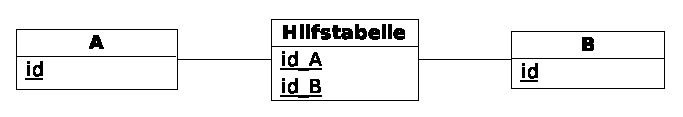
\includegraphics{img/NzuM}
\caption{$M:N$ Beziehung}
\label{nzum}
\end{center}
\end{figure}

\subsection{Reines Java}

\subsubsection{Modellierung}

Java Objektmengen kommen in drei grundlegenden Varianten: 

\begin{description}
\item[Set<\emph{E}>:]{Menge von \emph{E}-Objekten ohne Duplikate}
\item[List<\emph{E}>:]{geordnete Liste von \emph{E}-Objekten; Duplikate sind erlaubt}
\item[Map<\emph{K},\emph{V}>:]{$1:1$ Abbildung von \emph{K}-Objekten auf \emph{V}-Objekte}
\end{description}

F�r jede dieser Schnittstellen gibt es in \cite{javaapi} ausf�hrliche Garantien
zu Laufzeit und Speicherverhalten der tats�chlichen Implementierungen. Java
selbst liefert f�r die unterschiedlichen Anforderungen des Programmierers
Implementierungen auf Vektor-, Listen- und Hash\-ta\-bellen\-ba\-sis, die an
entscheidenden Stellen eben besser als die von der Schnittstelle geforderten
Kriterien sind. Bei besonderen Anforderungen k�nnen diese Schnittstellen auch
selbst oder von Drittanbietern implementiert werden.

Hier das Beispiel der Ordnerstruktur mit Hilfe eines
\code{Set}s:\label{java-unidirectional}
\begin{lstlisting}
package webbook;
class BasicFolder implements IFolder {
	/* Die Menge der Unterordner dieses Ordners */
	java.util.Set<IFolder> subfolders 
		= new java.util.HashSet<IFolder>();
	
	/* ... */
}
\end{lstlisting}

Diese Methode modelliert jedoch nicht die Symmetrie dieser Beziehung. In der
Navigation durch dieses Modell kann nicht direkt von einem Unterorder zu seinem
�berordner gesprungen werden. Daf�r m�sste die -- ebenfalls h�ndisch zu
implementierende -- Liste aller Ordner durchsucht werden.

Umgekehrt k�nnte das SQL-Modell �bernommen werden, um immer im Modell "nach oben"
navigieren zu k�nnen. 

\begin{lstlisting}
package webbook;
class BasicFolder implements IFolder {
	/* Der �bergordnete Ordner */
	IFolder parent = null;
	
	/* ... */
}
\end{lstlisting}

Somit kann der �bergeordnete Ordner festgestellt werden. Da Java
keine M�glichkeit bietet, �ber alle Instanzen einer Klasse zu iterieren, kann mit
dieser Methode -- ohne zus�tzlichen Programmieraufwand -- nicht einmal die Menge aller
enthaltenen Ordner festgestellt werden. Normalerweise werden daher beide
Richtungen implementiert. Da es sich dabei um redundante Informationen handelt,
muss bei Manipulationen dieser Struktur jedoch besondere Sorgfalt an den Tag
gelegt werden. Durch die Kapselung der Attribute kann das Problem jedoch auf die
betroffene Klasse beschr�nkt werden.

\begin{lstlisting}
package webbook.manual;
class Folder implements IFolder {
	/* Die Menge der Unterordner dieses Ordners */
	private java.util.Set<Folder> subfolders 
		= new java.util.HashSet<Folder>();
	/* Der �bergordnete Ordner */
	private Folder parent = null;

	public void setParent(Folder f)
	{
		/* Konsistenz�berpr�fung */
		if (f == this || (f != null && f.hasParent(this)) )
			throw new Exception("Konsistenzverletzung");

		/* entfernt diesen Ordner aus altem parent */
		if (parent != null)
			parent.removeFolder(this);

		/* f�gt diesen Ordner zum neuen parent hinzu */
		parent = f;
		if (parent != null)
			parent.addFolder(this);
	}

	/* rekursiver �berpr�fung der �berordnung */
	public bool hasParent(Folder p)
	{
		return parent == p || ( parent != null && parent.hasParent(p) );
	}

	/* ... */
}
\end{lstlisting}

Gleichzeitig k�nnen solche Methoden auch dazu benutzt, werden zus�tzliche
Konsistenz�berpr�fungen durchzuf�hren, wie hier die \code{hasParent} Methode,
deren �berpr�fung die Baumstruktur garantiert, da kein Zyklus gebildet werden
kann (\code{this} m�sste dazu bereits dem neuen �berordner �bergeordnet sein).

Andere Beziehungstypen k�nnen mit entsprechendem Aufwand mit passenden
Kombinationen von \code{Set}s und einfachen Attributen implementiert werden.

\subsubsection{Implementierung mit Datenbank}

Werden die betrachteten Objekte in einer Datenbank gespeichert, so m�ssen die
Beziehungen ebenfalls gespeichert werden. Dazu eignen sich die im vorhergehenden
Abschnitt besprochenen Fremdschl�ssel.

Um beim Laden aus der Datenbank nicht den kompletten Objektbaum holen zu m�ssen,
braucht man Beziehungen nicht automatisch mitladen, sondern l�dt die
verkn�pften Daten erst bei Zugriffen auf die Mengenattribute in die
Javaumgebung. 

Je nach Beziehungstyp und Darstellung in der Datenbank wird beim Speichern
einfach das betroffene Attribut �berschrieben oder der gesamte betroffene
Bereich der Relation wird gel�scht und neu geschrieben. Bei 
Beziehungen mit einer gro�en Anzahl von beteiligten Objekten lohnt es sich
speziellen Mengenklassen zu implementieren, die nur inkrementell die
durchgef�hrten �nderungen speichern.

Komplexere Abfragen auf Beziehungen werden direkt in SQL implementiert. Die
Ergebnisse k�nnen  dabei individuell an die Anforderungen angepasst werden.

\subsection{SimpleORM}

In \cite{simpleorm}, "Associations and Class Mappings", argumentiert Berglas,
dass reale Anwendungen soviel Kontrolle -- zum Beispiel f�r seitenweises
Anzeigen -- �ber die "zu $N$" Seite brauchen, dass besser die allgemeine
Suchfunktionen verwendet werden sollen, als diese Funktionen nochmals f�r diesen
Spezialfall zu implementieren. Daher unterst�tzt SimpleORM nur die "zu Eins"
Seite von Beziehungen direkt. Durch eine \code{SFieldReference} werden die
notwendigen Strukturen definiert. Hier die Definition der Eltern-Kind Beziehung
der Ordner:

\begin{lstlisting}
package webbook.simpleorm;
public class Folder implements IFolder {
	// Referenz auf den �bergeordneten Ordner
	public final SFieldReference PARENT = new SFieldReference(meta, meta, "ref");

	public Folder getParent() {
		return (Folder)getObject(PARENT);
	}

	public void setParent(Folder parent) {
		setObject(PARENT, parent);
	}
\end{lstlisting}

Dank der h�heren Abstraktionsebene von SimpleORM operiert die Klasse nun direkt
auf \code{Folder}-Instanzen. Damit wird schon bei der Verarbeitung in der
Javaapplikation die Konsistenz der Datenbank garantiert. Die Zyklusfreiheit des
Graphen kann durch die oben vorgestellte \code{hasParent} Methode �berpr�ft
werden:

\begin{lstlisting}
package webbook.simpleorm;
public class Folder implements IFolder {
	public void validateField(SFieldMeta field, Object newValue) {
		if (field == PARENT) {
			if (newValue == null)
				return;

			if (!newValue instanceof Folder)
				throw new SValidationException("unerwarteter Objekttyp");

			if (newValue == this || ((Folder)newValue).hasParent(this))
				throw new SValidationException("Konsistenzverletzung");

			// Alle Bedingungen erf�llt
			return;
		}
	}
\end{lstlisting}

Um alle Unterfolder zu erhalten, befragt man die Datenbank:

\begin{lstlisting}
public class Folder implements IFolder {
	public List<Folder> getChildren() {
		SResultSet result = Folder.meta.newQuery().eq(Folder.PARENT, this)
			.descending(Folder.TITLE).execute();
		return Collection.unmodifiableList(result.getArrayList(1000));
	}
\end{lstlisting}

Bei der Modellierung der Schnittstelle nach au�en stellen sich nat�rlich die
gleichen Probleme wie bei reinem Java. Der minimalistische Ansatz von SimpleORM
l��t bei der Implementierung jedoch keine Mi�verst�ndnisse zu. Die Beziehung ist
�ber das \code{PARENT} Feld definiert. \code{add}- und \code{remove}-Methoden
brauchen sich daher auch nur um dieses k�mmern. �nderungen am Abfrageergebnis
aus \code{getChildren()} k�nnen daher keine Auswirkung auf die Datenbank haben.
Um das auch an Benutzer dieser Klassen zu kommunizieren, kann mit
%% f�r silbentrennung:
\emph{Collection.unmodifiableList()} eine nur-Lesen Liste erzeugt werden, die
bei Schreibversuchen eine Ausnahmebedingung erzeugt. 

Eine Spezialit�t von SimpleORM ist die Notwendigkeit einer oberen Schranke f�r
die Anzahl der Ergebnisobjekte bei der \code{getArrayList} Methode. Im
Quelltext wird dies mit der Fr�herkennung unbeschr�nkter Abfragen begr�ndet.
Dar�ber hinaus ist es aber auch sinnvoller, gro�e Ergebnismengen zeilenweise
abzuarbeiten, da bereits bearbeitete Objekte wieder freigegeben werden k�nnen.

\subsection{Hibernate}

In der XML-Abbildungsbeschreibung werden $1:N$ und Mengenbeziehungen direkt mit
eigenen Elementen unterst�tzt. Dadurch ergibt sich eine sehr komfortable
Modellierung dieser Sachverhalte.

Die Menge der Schlagworte wird mit einem \xml{<set/>} beschrieben:
\begin{lstlisting}[language=xml]
<set name="tags" cascade="all">
	<key column="id"/>
	<element column="tag" type="webbook.hibernate.utils.TagType" not-null="true"/>
</set>
\end{lstlisting}

Hibernate erzeugt aus dieser Definition automatisch die Tabelle \sql{tags} mit
den Spalten \sql{id} und \sql{tag}. Da die Schlagwortmenge kein eigenst�ndiges
Objekt ist, sondern immer nur im Kontext des beschlagworteten Artefakts
existiert, wird durch \xml{cascade="all"} angezeigt, dass alle Operationen auf
dem �bergeordneten Element -- vor allem �nderungen am Schl�sselwert und L�schung
-- auch auf diesem \xml{<set/>} durchgef�hrt werden sollen.

Hibernate kennt auch \xml{<list/>}, \xml{<array/>} und \xml{<primitive-array/>}
f�r angeordnete Daten mit unterschiedlichen Javarepr�sentationen, \xml{<map/>}
f�r 2-Tupel und \xml{<bag/>} f�r ungeordnete Multimengen.

Beziehungen zwischen Objekten werden mit den Elementen \xml{<one-to-many/>},
\xml{<many-to-} \xml{one/>} und \xml{<many-to-many/>} beschrieben. Die $:N$ Varianten
m�ssen dabei in einer Mengendefinition eingebettet werden, um die Semantik der
Beziehung zu spezifizieren. Von den eingeschr�nkten M�glichkeiten der
Modellierung in reinem Java erbt auch Hibernate die Assymetrie von Beziehungen.
Die beiden Enden m�ssen seperat modelliert werden. Hier wieder am Beispiel der
Ordner:
\begin{lstlisting}[language=xml]
<many-to-one name="parent" class="Folder"/>
<set name="children" inverse="true">
	<key column="id"/>
	<one-to-many class="Folder"/>
</set>
\end{lstlisting}

Dabei verhindert die \xml{inverse="true"} Deklaration, dass �ber die
\code{children} Menge die Beziehung ver�ndert werden kann. Die \code{children}
Menge muss auf der Javaseite wie schon bei der Implementierung mit reinem JDBC
beschrieben gepflegt werden.

\section{Datenbankverbindung und -abfragen}

\subsection{SQL}

Der direkte Zugriff auf die Datenbank erfolgt entweder mit SQL-Befehlen auf
einem eigenen kommandozeilenorientierten Klienten oder mit einer
Verwaltungsapplikation, die auch Unterst�tzung in der Verwaltung und Wartung
des Datenbankschemas sowie der Erstellung von Abfragen bietet.

\subsection{Reines Java}

Die JDBC API unter Java ist eine gemeinsame Schnittstelle f�r den
Datenbankzugriff. Um die verschiedenen Kommunikationsprotokolle zu unterst�tzen,
wird von den jeweiligen Datenbankherstellern auch ein JDBC-Treiber zur Verf�gung
gestellt.

Ein typischer Verbindungsablauf sieht so aus:

\begin{lstlisting}[numbers=left]
Class.forName(TREIBER); // registrieren
Connection connection = DriverManager.getConnection(URL); // verbinden
PreparedStatement stmt = connection.prepareStatement(SQL);
stmt.set<<Type>>(INDEX, VALUE); // Parameter setzen
stmt.execute(); // Abfrage durchf�hren
ResultSet rs = stmt.getResultSet();
while(rs.next()) { // Cursor bewegen
	rs.get<<Type>>(INDEX); // Werte abfragen
}
// Resourcen explizit freigeben
rs.close();
stmt.close();
connection.close();
\end{lstlisting}

Zuerst l�dt \code{Class.forName("JDBC-Treiber")} den JDBC-Treiber in die
virtuelle Maschine (Zeile~1). Danach �ffnet
\code{DriverManager.getConnection("URL")} die Verbindung \code{conn} zur
Datenbank (Zeile~2). Optional werden �ber diesen Aufruf weitere Parameter an den
Treiber �bergeben. 
Die Anweisung \code{conn.prepareStatement(SQL)} erzeugt aus der SQL-Abfrage
ein parameterisiertes, wiederverwertbares Kontainerobjekt (Zeile~3) in dem
\code{set}-Aufrufe Parameter verschiedener Typen setzen (Zeile~4).
\code{execute()} �bertr�gt die Abfrage und die Parameter an die
Datenbank, wo sie direkt interpretiert und ausgef�hrt wird (Zeile~5). Als Ergebnis erh�lt
man ein \code{ResultSet}, eine Repr�sentation eines Datenbankcursors (Zeile~6).
Parallel zu den \code{set}-Methoden des \code{PreparedStatement}s hat das
\code{ResultSet} \code{get}-Methoden, die Attribute in verschiedenen Datentypen
auslesen.

\subsection{SimpleORM}

Diese Bibliothek �bernimmt die Verwaltung, jedoch nicht die Erstellung der
JDBC-Verbindung. Auch hier l�dt zuerst \code{Class.forName("JDBC-Treiber")} den
JDBC-Treiber in die virtuelle Maschine (Zeile~1). \code{SConnection} �bernimmt
nun die direkte Verwaltung der JDBC-Verbindung (Zeile~2-4). 

\begin{lstlisting}[numbers=left]
Class.forName(TREIBER); // registrieren
SDataSource ds = new SDataSource(URL, new Properties());
SConnection.attach(ds, "default"); // verbinden
SConnection.begin();
\end{lstlisting}

Wenn die Verbindung steht, k�nnen Standardabfragen nach dem Prim�rschl�ssel
automatisiert mit \code{mustFind(PRIMARY\_KEY)} erzeugt werden. �ber die
\code{SQuery} Schnittstelle k�nnen komplexere Anfragen programmatisch gebaut
werden.

\subsection{Hibernate}

Die Datenbankverbindung von Hibernate wird �ber eine XML-Datei konfiguriert.

\begin{lstlisting}[language=xml,numbers=left]
<hibernate-configuration>
	<session-factory>
		<!-- Databankverbindungsparameter -->
		<property name="connection.driver_class">JDBC-TREIBER</property>
		<property name="connection.url">URL</property>
		<!-- SQL Dialekt -->
		<property name="dialect">org.hibernate.dialect.PostgreSQLDialect</property>
		<!-- ... -->
		<!-- Schema Definition einbinden -->
		<mapping resource="webbook/hibernate/DataObject.hbm.xml"/>
\end{lstlisting}

Wie bei den anderen Bibilotheken auch, liegt hier eine JDBC-Verbindung zu
Grunde. Der Treiber und die URL daf�r werden mit \xml{connection.driver\_class}
und \xml{connection.url} angegeben (Zeile~4,5). Damit Hibernate korrekt
optimierte SQL-Definitionen und Abfragen erzeugt, gibt der \xml{dialect} auf
Zeile~7 den -- f�r die Tests verwendeten -- \code{PostgreSQLDialect} an. Zuletzt
werden �ber \xml{mapping}-Elemente die einzelnen Abbildungsdefinitionen
eingebunden (Zeile~10). �ber weitere \xml{property}-Elemente k�nnen zus�tzliche
Parameter von Hibernate konfiguriert werden.

Da die Konfiguration von Hibernate �ber die XML-Datei l�uft, enth�lt der
Quelltext keine Parameter mehr, Objekte k�nnen direkt �ber Javakonstrukte
angesprochen werden:

\begin{lstlisting}[numbers=left,columns=fullflexible]
// hibernate.cfg.xml einlesen
SessionFactory sessionFactory = new Configuration().configure().buildSessionFactory();

// Abfrage nach Prim�rschl�ssel
Object result = sessionFactory.getCurrentSession().get(KLASSE, ID);

// beliebige Abfragen
List results = sessionFactory.getCurrentSession().createQuery(
	"from NAME join NAME.tags where CONDITION").list();
\end{lstlisting}

Hibernate bringt eine eigene, SQL-�hnliche Abfragesprache mit, die in der
letzten Anweisung gezeigt wird. 

\section{Datensicherheit}
\label{datensicherheit}

Die in Abschnitt~\ref{ACID} aufgelisteten Forderungen sollten nat�rlich auch im
Objektmodell halten. Welche Vorkehrungen die einzelnen Systeme daf�r haben,
wird im folgenden Abschnitt besprochen.

\subsection{SQL}

In SQL k�nnen mehrere Anweisungen zu einer Transaktion zusammengefasst werden.
Die Anweisungen einer Transaktion werden entweder alle gemeinsam oder �berhaupt
nicht ausgef�hrt. Eine Transaktion wird mit dem Befehl \sql{BEGIN} ge�ffnet und
mit \sql{COMMIT WORK}
abgeschlossen. Das Datenbanksystem garantiert mit dem erfolgreichen Abschluss
der Transaktion deren Dauerhaftigkeit. Kommt es zu einem Fehler, kann die
Transaktion mit dem Befehl \sql{ROLLBACK WORK} abgebrochen werden.

Das sogenannte Isolationslevel beschreibt die (Un-)Abh�ngigkeit von
Transaktionen untereinander. Starke Isolierung von parallel ablaufenden
Anweisungen erfordert einen gewissen Aufwand auf Seiten des Datenbanksystems.
Durch die Angabe eines niedrigeren Isolationslevels verzichtet man auf nicht
ben�tigte Mechanismen. Das sollte nat�rlich nur gemacht werden, wenn die
Anwendung auch ohne diese Zusicherungen korrekt funktioniert.

Die beiden wichtigsten Isolationslevels sind \sql{READ COMMITTED}
und \sql{SERIALIZABLE}. Mit \sql{READ COMMITTED} Isolation sieht jede Anweisung
nur Datans�tze aus bereits abgeschlossenen Transaktionen. Innerhalb einer
Transaktion kann es jedoch vorkommen, dass beim neuerlichen Lesen eines
Datensatzes auch neue, ge�nderte Daten gelesen werden, wenn von einer
parallelen Transaktion dieser Datensatz ge�ndert wurde. Damit sichert
\sql{READ COMMITTED} einen konsistenten Blick auf die Datenbank \emph{innerhalb
einer einzelnen Anweisung} zu. Mit
%% Silbentrennung
\emph{SERIALIZABLE} Isolation verh�lt sich die
Datenbank so, als w�rden alle Transaktionen strikt nacheinander ausgef�hrt
werden. Je nach Implementierung in der Datenbank kommt es dadurch zu verst�rkten
Wartezeiten auf den benutzten Tabellen- und Zeilensperren oder zu erzwungenen
Transaktionsabbr�chen bei Schreibkonflikten (wie bei MVCC in
Abschnitt~\ref{mvcc} beschrieben).

\subsection{Reines Java}

In der Standardkonfiguration befindet sich JDBC im \emph{autocommit}-Modus.
Dabei wird nach jeder SQL-Anweisung automatisch die aktuelle Transaktion
abgeschlossen und
eine neue er�ffnet. Muss eine Applikation mehrere Anweisungen gemeinsam in
einer Transaktion abwickeln, so kann der autocommit-Modus mit
\code{conn.setAutoCommit(false);} deaktiviert werden. Die gesamte Struktur
einer Transaktion sieht dann so aus:
\begin{lstlisting}[columns=fullflexible,numbers=left]
public static void machWas(java.sql.Connection conn)
	throws java.sql.SQLException
{
	conn.setAutoCommit(false);
	
	try {
	
		/* Datenbankanweisungen hier */

		conn.commit();
	} catch (Throwable t) {
		conn.rollback();
		throw t;
	}
}
\end{lstlisting}

Das Deaktivieren des automatischen Transaktionsabschlusses in Zeile~4 er�ffnet
gleichzeitig eine neue Transaktion. Danach kann im \code{try}-Block die
Datenbank �ber JDBC-Aufrufe abgefragt und modifiziert werden (Zeile~8). Ist
alles korrekt abgelaufen, schliesst \code{conn.commit()} die Transaktion ab
(Zeile~10). Kommt es zu einem Fehler, bricht \code{conn.rollback()} die
Transaktion ab (Zeile~12), bevor \code{throw t} den Fehler weiterreicht
(Zeile~13). Situationsabh�ngig kann hier auch versucht werden, den Fehler
lokal zu behandeln, zum Beispiel durch das Neustarten der Transaktion.

Es ist dabei auf die Synchronisation zwischen den verschiedenen Ausf�hrungsstr�ngen der
Java-Applikation zu achten, da diese die M�glichkeit haben sich gegenseitig auf
der JDBC-Verbindung zu st�ren. Normalerweise wird dieses Problem umgangen, indem
f�r mehrere Threads jeweils eigene Verbindungen ge�fnet werden.

\subsection{SimpleORM}

Die JDBC-Verbindung wird in eine \code{SConnection} Instanz geh�llt. Diese
Instanz ist Thread-lokal. Damit wird die gesamte Synchronisation zwischen
Threads an das DBMS delegiert. Transaktionen k�nnen �ber die Methoden
\code{begin()}, \code{rollback()} und \code{commit()} gesteuert werden:

\begin{lstlisting}
SConnection.begin();

try {
	/* Datenbankmodifikationen */

	SConnection.commit();
} catch (Throwable t) {
	SConnection.rollback();
	throw t;
}
\end{lstlisting}

\code{SRecordInstance}s sind jedoch an die Lebenszeit einer Datenbanktransaktion
gebunden, da au�erhalb einer Transaktion die Konsistenz zur Datenbank nicht
gew�hrleistet werden kann. Will man solche Objekte ausserhalb einer Transaktion
verwenden, zum Beispiel um sie via RMI zu transportieren, kann man mit
\code{INSTANZ.detach()} den Record von der Transaktion l�sen. Dabei aktiviert
SimpleORM automatisch optimistische Sperrmechanismen, um auch �ber die
Datenbanktransaktion hinaus Inkonsistenzen feststellen zu k�nnen.
\code{INSTANZ.attach()} f�gt einen Record in die aktuelle Transaktion wieder
ein.

\subsection{Hibernate}

Das Hibernate Gegenst�ck zur JDBC-Verbindung, ist die \code{Session}. In ihr wird
die Verbindung zur Datenbank aufgebaut und die einzelnen Transaktionen
abgehandelt. Die Hibernate Dokumentation empfiehlt entweder eine Session pro
Anfrage in einem Client/Server System zu verwenden oder eine Session f�r die
Abwicklung eines ganzen Gesch�ftsfalls zu verwenden. Im zweiten Fall werden die
Objekte automatisch versioniert und beim Abschluss einer Transaktion
optimistisch in die Datenbank zur�ckgeschrieben. Dadurch werden keine Sperren
in der Datenbank gebraucht, es kann jedoch bei Schreibkonflikten zu einem
erzwungenen Transaktionsabbruch kommen. Um diese zu vermeiden, kann man an
einer bekannten Stelle in der Datenbank vermerken, welche Objekte gerade "in
Arbeit" sind und
so bereits beim ersten Zugriff verhindern, dass es zu solchen erzwungenen
Abbr�chen kommt.

\begin{lstlisting}
Transaction trans = sessionFactory.getCurrentSession().getTransaction();
trans.begin();

try {
	/* Datenbankmodifikationen */

	trans.commit();
} catch (Throwable t) {
	trans.rollback();
	throw t;
}
\end{lstlisting}

\section{Objektlebenszyklus}

Der typische Lebenszyklus eines Objektes besteht aus seiner Erzeugung, einer
beliebigen Abfolge von Lese- und Modifikationsoperationen und endet mit der
L�schung des Objektes. Das wird in der Literatur im Akronym CRUD, engl. f�r
Create, Read, Update, Delete, zusammengefasst. Hier zeigt sich der erste gro�e
Vorteil der Bibliotheken gegen�ber der manuellen Implementierung, da diese
Operationen aus den bisher definierten Strukturen automatisch abgeleitet werden
k�nnen.

\subsection{SQL}

Die SQL Anweisung \sql{INSERT INTO Tabelle (Spalten) VALUES (Werte)} ist die Grundform der
Objekterzeugung. Dabei wird eine neue Zeile in \sql{Tabelle} mit den
angegeben Werten geschrieben.

Um Objekte aus der Datenbank zu lesen, k�nnen mit \sql{SELECT}-Abfragen
beliebig komplexe Relationen und Bedingungen spezifiziert werden.

\sql{UPDATE Tabelle SET Spalte1=Wert1, Spalte2=Wert2 WHERE Bedingung} �ndert
die angegebenen Attribute in \sql{Tabelle} bei allen Tupeln, die \sql{Bedingung}
erf�llen.

\sql{DELETE FROM Tabelle WHERE Bedingung} l�scht alle Zeilen, die \sql{Bedingung}
erf�llen.

Ergebnisse werden in tabellarischer Form zur�ckgegeben. Die genau Darstellung
h�ngt von der benutzten Software ab.

\subsection{Reines Java}

�ber \code{java.sql.Statement}s oder \code{java.sql.PreparedStatement}s k�nnen
SQL-Anweisungen direkt an die Datenbank abgesetzt werden. Das Ergebnis wird
durch ein \code{java.sql.ResultSet} repr�sentiert.

\subsubsection{Schnittstelle}

Will man die Koppelung zwischen Gesch�ftslogik und Persistenz gering halten,
empfiehlt sich eine strikte Trennung der beiden Teile durch die Einrichtung
einer eigenen
Datenzugriffschicht\footnote{engl.: DAL, Data Access Layer}. Dabei ist zwischen
den Datenbank- und den Objektoperationen zu unterscheiden:
\begin{lstlisting}[columns=fullflexible,numbers=left]
public interface IDatabase
{
	public abstract void connect();
	public abstract void begin();
	public abstract void executeSQL(String sql) throws SQLException;
	public abstract void rollback();
	public abstract void commit();
	public abstract void disconnect();
}

public interface IDriver<OBJ extends IDataObject>
{

	/** Objekt erzeugen */
	public abstract OBJ createObject();
	/** Objekt abspeichern */
	public abstract OBJ saveObject(OBJ o) throws SQLException;

	/** Objekt nach Prim�rschl�ssel suchen */
	public abstract OBJ findById(int id) throws SQLException;
	/** Objekt nach Schl�sselw�rtern suchen */
	public abstract Set<? extends OBJ> findByTags(TagExpression tags) throws SQLException;

	/** Objekt l�schen */
	public abstract void deleteById(int id) throws SQLException;
	public abstract void deleteObject(OBJ o) throws SQLException;

}
\end{lstlisting}

\subsubsection{Suchen und Laden}

Der einfachste Fall ist das Laden eines \code{Article}s nach seinem
Prim�rschl�ssel:
\begin{lstlisting}[columns=fullflexible,numbers=left]
public class ArticleDAL extends BaseDAL implements IDAL<Article> {

	public Article findById(int id) throws SQLException
	{
		PreparedStatement stmt = _conn.prepareStatement(
			"SELECT * FROM articles WHERE id = ?");
		stmt.setInt(1, id);
		ResultSet result = stmt.executeQuery();
	
		if (result.next())
			return loadFrom(result);
		else
			return null;

	}
\end{lstlisting}

In Zeile~5-7 wird die SQL Anweisung vorbereitet und ausgef�hrt. Wenn ein
Artikel mit dieser ID existiert (Zeile~9), dann l�dt
\code{BaseDAL.loadFrom(ResultSet)} die Attribute aus dem \code{ResultSet} in
eine neue Instanz. \code{loadFrom} ist eine virtuelle Methode, bei der die
Basisimplementierung in \code{BaseDAL} die \code{IDataObject}-Attribute l�dt,
w�hrend \code{ArticleDAL.loadFrom} die zus�tzlichen Attribute des Artikels
ausliest. Das \code{PreparedStatement} kann auch wiederverwendet werden, wie
das n�chste Beispiel zeigt.

\subsubsection{Schreiben}

Hier die Methode, um einen neuen \code{Article} in die Datenbank zu speichern:
\begin{lstlisting}[columns=fullflexible,numbers=left]
	private PreparedStatement	_getNewId	= null;
	private PreparedStatement	_insertArticle	= null;

	protected void insertObject(Article obj) throws SQLException
	{
		if (_getNewId == null) {
			_getNewId = getConnection().prepareStatement(
				"select nextval('articles_id_seq')");
		}
		_getNewId.execute();
		ResultSet rs = _getNewId.getResultSet();
		rs.next();
		obj.setId(rs.getInt(1));
	
		if (_insertArticle == null) {
			_insertArticle = getConnection().prepareStatement(
				"INSERT INTO articles (created_on, last_modified, title, text, summary, id)\n"
				+ "VALUES (?, ?, ?, ?, ?, ?)");
		}
		// prepareSave(obj, _insertArticle):
		{
			_insertArticle.setTimestamp(1, new Timestamp(obj.getCreatedOn().getTime()));
			_insertArticle.setTimestamp(2, new Timestamp(obj.getLastModified().getTime()));
			_insertArticle.setString(3, obj.getTitle());
			_insertArticle.setString(4, obj.getText());
			_insertArticle.setString(5, obj.getSummary());
			_insertArticle.setInt(6, obj.getId());
		}
		_insertArticle.execute();
	}
\end{lstlisting}

Das zentrale St�ck hier ist die \sql{INSERT}-Anweisung (Zeile~17,18) und das
Bef�llen der Parameter (Zeile~20-28). Durch geschicktes Anordnen der Parameter
in der SQL-Anweisung k�nnen die \code{set}-Anweisungen bei \sql{INSERT} und
\sql{SELECT} gemeinsam genutzt werden, wie hier mit dem \code{prepareSave}
\label{prepareSave} Kommentar angedeutet ist (Zeile~20). Aufgrund der fehlenden
Unterst�tzung f�r benannte Parameter von \code{Statement}s ist dabei besonders
auf die korrekte Reihenfolge der Platzhalter und Attribute zu achten.

Die ben�tigten SQL-Anweisungen werden in Instanzvariablen als
\code{PreparedStatement} gespeichert und erst bei der ersten Benutzung
initialisiert (Zeile~1,2,7,16). Das erm�glicht dem JDBC-Treiber, die
SQL-Anweisung einmalig im Datebankserver in optimierter Form abzulegen.
Nachfolgende Aufrufe �bertragen nur noch die Parameter und ersparen sich somit
das wiederholte Parsen und Optimieren der Anweisung.

Am Anfang der Methode ist ein Block um einen eindeutigen ID f�r den neuen
Artikel aus der Datenbank abzufragen (Zeile~6-13). Dadurch kann sichergestellt
werden, dass ein eindeutiger ID benutzt wird, ohne die ganze Tabelle sperren zu
m�ssen. Alternativ k�nnen auch UUIDs\footnote{Universally Unique IDentifier}
eingesetzt werden. Diese sind sogar �ber unabh�ngige System hinweg eindeutig,
bestehen aber aus 128 Bit und sind daher in der Bearbeitung teurer. UUIDs sind
in \cite{DCE} definiert.

\subsubsection{L�schen}

Objekte werden mit einer einfachen \sql{DELETE} Anweisung gel�scht. Die
Java-Methode dazu gleicht in der Struktur den bisher vorgestellten Methoden.

\subsection{SimpleORM}

Um die Werkzeuge vergleichbar zu halten, implementiert auch der SimpleORM Test
die gleichen Schnittstellen wie zuvor vorgestellt. Aufgrund der direkten Koppelung zur
Persistenzschicht durch die Ableitung von \code{SRecordInstance} sind die
meisten Methoden der \code{IDAL} Schnittstelle nur Weiterreichungen an
\code{SRecordInstance} Methoden des betroffenen Objektes. Diese werden hier
vorgestellt.

\subsubsection{Suchen und Laden}

Zuerst wieder das Auffinden eines Objektes nach seinem Prim�rschl�ssel:
\begin{lstlisting}
public Article findById(int id)
{
	// Das ist wirklich so einfach:
	return (Article) Article.meta.find(new Integer(id));
}
\end{lstlisting}
Damit erstellt die SimpleORM Bibliothek automatisch die notwendigen
SQL-Abfragen und erzeugt ein bef�lltes Java Objekt. Um auf die Attribute
zugreifen zu k�nnen, ist es notwendig, auf die \code{SRecordInstance}
zuzugreifen. F�r den Titel sieht das so aus:
\begin{lstlisting}
public class DataObject extends SRecordInstance {
	public static final SFieldString TITLE
		= new SFieldString(meta, "title", -1, SSimpleORMProperties.SMANDATORY.ptrue());

	public String getTitle()
	{
		return getString(TITLE);
	}

	public void setTitle(String title)
	{
		setString(TITLE, title);
	}
\end{lstlisting}
\code{getString} und \code{setString} sind dabei Funktionen der
\code{SRecordInstance}, die das angegebene Feld bearbeiten. Aufgrund der
Metainformationen im \code{SFieldString} Objekt k�nnen bereits beim Setzen des
Feldes Randbedingungen wie Typ, Wertebereich oder benutzerspezifische
Validierungsregeln �berpr�ft werden.

\subsubsection{Schreiben}

\code{SConnection.commit()} �bertr�gt alle ausstehenden �nderungen an die
Datenbank und schliesst die Transaktion ab. Soll ein Objekt fr�hzeitig in die
Datenbank geschrieben werden -- zum Beispiel, um in einer nachfolgenden Abfragen
innerhalb der gleichen Transaktion aufzuscheinen, kann die Methode \code{flush}
der \code{SRecordInstance} verwendet werden.

\subsubsection{L�schen}

Die \code{SRecordInstance.deleteRecord()} Methode markiert ein Objekt als
gel�scht. Mit dem Abschluss der Transaktion wird es auch in der Datenbank
gel�scht.

\subsection{Hibernate}

Um die Werkzeuge vergleichbar zu halten, implementiert auch der Hibernate Test
die gleichen Schnittstellen wie zuvor vorgestellt. 

\subsubsection{Suchen und Laden}

Wie auch bei SimpleORM ist die Abfrage nach dem Prim�rschl�ssel sehr einfach
und erzeugt ebenfalls gleich die notwendigen Java Objekte.
\begin{lstlisting}
public Article findById(int id)
{
	// Das ist wirklich so einfach:
	return (Article)sessionFactory.getCurrentSession().get(Article.class, id);
}
\end{lstlisting}

\subsubsection{Schreiben und L�schen}

Mit den \code{saveOrUpdate(OBJEKT)} und \code{delete(OBJEKT)} Methoden der
\code{Session} k�nnen Objekte in die Datenbank geschrieben oder gel�scht werden.


\section{Ableitung}
\label{ableitung}

Selbst in so einfachen Systemen wie der \code{webbook} Beispieldatenbank kann
mit einer passenden Klassenhierarchie doppelter Programmtext vermieden werden.
Alle Klassen der \code{webbook} Beispieldatenbank haben die Attribute der
\code{IDataObjekt} Schnittstelle gemein. Diese Attribute in einer gemeinsamen
Basisklasse zu verwalten reduziert den Programmieraufwand und verhindert
Inkonsistenzen in der Definition zwischen den Klassen.

\TODO{Literatursuche: OO-Design: Warum Ableiten?}

\subsection{SQL}

F�r verschiedene Modellierungs- und Leistungsanforderungen gibt es
unterschiedliche Ans�tze, um Ableitungshierarchien abzubilden. Da die korrekte
Auswahl des Ansatzes wichtig ist, um die f�r die Applikation notwendigen
Abfragen effizient durchf�hren zu k�nnen, hat sich hier kein einzelner
"bester" Ansatz herauskristallisiert.

\subsubsection{Tabelle pro konkreter Klasse}

Ein sehr direkter Ansatz zur Abbildung einer Klassenhierarchie ist der Einsatz
einer eigenen Tabelle f�r jede Klasse, von der direkt
Instanzen\footnote{typischerweise nur Bl�tter im Ableitungsbaum} erzeugt
werden. Abbildung~\ref{concrete} illustriert das.

\begin{figure}
\begin{center}
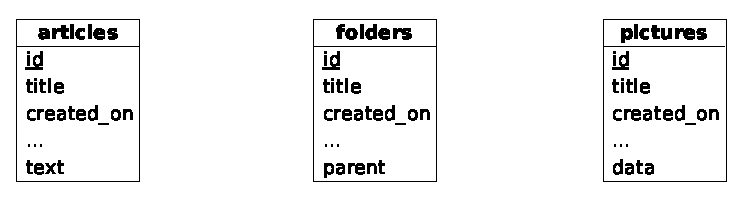
\includegraphics{img/concrete}
\caption{Tabelle pro konkreter Klasse}
\label{concrete}
\end{center}
\end{figure}

\paragraph{Vorteile:} Durch die direkte Abbildung ist dieser Ansatz der
einfachste der hier vorgestellten und erzwingt keine Koordination der
Objektklassen auf der Applikationsseite. So erfordert zum Beispiel das
Hinzuf�gen neuer Unterklassen keine �nderungen an vorhandenen Strukturen und
bei �nderungen an bestehenden Attributen ist der Implementierungsaufwand auf
die direkt betroffenen Tabellen und Klassen beschr�nkt.

Abfragen auf einzelne Klassen/Tabellen werden ebenfalls unmittelbar umgesetzt
und k�nnen mit minimalem Aufwand in der Datenbank auch tabellenspezifisch
optimiert werden, ohne Interferenzen auszul�sen. Aufgrund der separaten Tabellen
bleiben Transaktionen auf die von ihnen direkt betroffenen Hierarchieteile
eingeschr�nkt.

\paragraph{Nachteile:} Bei jeder Abfrage m�ssen alle beteiligten konkreten
Klassen bekannt sein, da danach die Tabellen ausgew�hlt werden.

Datenbankanweisungen, die zentrale Attribute betreffen -- Abfragen und
Daten�nderungen -- m�ssen auf mehrere Tabellen zugreifen. Das wiederum
erfordert einen Mehraufwand pro Tabelle in Form von l�ngeren Anweisungen
und mehrfachen Indexzugriffen. 

Da es keinen gemeinsamen Prim�rschl�ssel gibt, muss bei polymorphen Abfragen
zur Klassenunterscheidung eine k�nstliche Typspalte erzeugt werden. Dabei
k�nnen Attribute je nach Position in der Ableitungshierarchie nicht oder nur
schwer polymorph abgefragt werden. Ebenfalls aufgrund des fehlenden
gemeinsamen Prim�rschl�ssels k�nnen Fremdschl�ssel nur als Verweis auf eine
konkrete Klasse definiert werden. Polymorphe Relationen k�nnen so entweder als
un�berpr�fte Konvention �ber ein Hilfskonstrukt wie das oben erw�hnte
k�nstliche Typattribut angelegt werden, oder indem f�r jede Unterklasse wiederum
eine eigene, verweisende Tabelle angelegt wird.

Bei �nderungen an gemeinsamen Attributen m�ssen alle Tabellen einzeln
modfiziert werden. Es gibt dabei keine Absicherung gegen unbeabsichtigte
Inkonsistenzen in der Struktur der einzelnen Tabellen.

\paragraph{Einsatzgebiet:} Dieses Schema eignet sich besonders f�r kleine
Objektmodelle wie die
%% Silbentrennung
\emph{webbook}-Datenbank, in der polymorphe Abfragen oder
Relationen nur eine geringe Rolle spielen aber die einfachen Strukturen dem
Verst�ndnis f�rderlich sind.

Hier einige beispielhafte Abfragen:
\begin{lstlisting}[language=sql]
-- einfache Abfrage nach Prim�rschl�ssel
SELECT * FROM articles WHERE id = ?

-- polymorphe Abfrage mit k�nstlicher Typspalte
-- spezielle Attribute m�ssen separat nachgeladen werden
SELECT 'articles'	AS class, id, created_on FROM articles WHERE -- ...
UNION ALL
SELECT 'pictures'	AS class, id, created_on FROM pictures WHERE -- ...
UNION ALL
SELECT 'folders'	AS class, id, created_on FROM folders WHERE -- ...
\end{lstlisting}

\subsubsection{Tabelle pro Klasse}

Mit $1:1$ Beziehungen wird der Ableitungsbaum direkt auf Tabellen
abgebildet. Attribute werden jeweils in der "allgemeinsten" Tabelle abgelegt.

Im Gegensatz zum "Tabelle pro konkreter Klasse" Schema sind hier die
Prim�rschl�ssel in der gesamten Hierarchie eindeutig, und Attribute von Knoten
des Ableitungsbaumes werden nur einmal definiert.

\begin{figure}
\begin{center}
\includegraphics{img/per-class}
\caption{Tabelle pro Klasse}
\label{per-class}
\end{center}
\end{figure}

\paragraph{Vorteile:} Dieser Ansatz bildet die Objekte nicht nur als
Attributslisten ab, sondern erfasst auch die Struktur der Ableitungshierarchie.
Dadurch sind polymorphe Abfragen auf den inneren Knoten des Ableitungsbaumes
m�glich. Eine typische polymorphe Abfrage in der Beispieldatenbank k�nnte die
Suche von Artefakten nach Worten aus dem Titel sein. Bei einer solchen Abfrage
ist der tats�chliche Typ des gefundenen Objekts zweitrangig. Da "Titel" ein
Attribut der Basistabelle \sql{data\_objects} ist, gen�gt eine einfache Abfrage
auf das \sql{title} Attribut.

Durch die Abbildung der Ableitungshierarchie gibt es nun auch einen gemeinsamen
Prim�rschl�ssel: \sql{data\_objects.id}. Dadurch k�nnen nun Fremdschl�ssel auf
beliebige Teilb�ume der Hierarchie referenzieren, indem die \sql{id} Spalte aus
der entsprechenden Tabelle angegeben wird.

Bei globalen Modifikationen in und an der Datenbank gibt es aufgrund der
geringen Strukturredundanz weniger M�glichkeiten, inkonsistente Manipulationen
durchzuf�hren. Speziell bei gr��eren Schemata und dem Hinzuf�gen oder Entfernen
von Attributen kann hier Aufwand gespart werden. Wie beim
Tabelle-pro-konkreter-Klasse Ansatz bleiben die Auswirkungen von solchen
�nderungen auf die direkt
betroffenen Klassen und Tabellen beschr�nkt und neue Unterklassen verursachen
keine �nderungen an vorhandenen Strukturen.

\paragraph{Nachteile:} Da die Attribute eines einzelnen Objektes �ber mehrere
Tabellen verteilt sind, multipliziert sich damit auch der Aufand an diese Daten
heranzukommen. Bei jeder Lese- oder Schreiboperation m�ssen die verschiedenen
Tabellen extra verkn�pft werden. Das bedeutet auch, dass der Benutzer der
Datenbank diese Strukturen kennen muss. 

Ein anderer gravierender Nachteil ergibt sich in einer Schw�che der
Datenbankbeschr�nkungen von SQL. Dort k�nnen Eindeutigkeitsbeschr�nkungen
nur auf einzelne Tabellen gelegt werden. Ohne zus�tzliche Attribute oder
Triggermethoden kann daher nicht verhindert werden, dass eine fehlerhafte
Anwendung ein Objekt mit Attributen mehrerer Klassen erzeugt, zum Beispiel,
indem Eintr�ge in der \sql{pictures} und der \sql{articles} Tabelle auf ein
gemeinsames \sql{data\_object} verweisen.

Durch die gemeinsamen Basistabellen blockieren sich Tabellensperren f�r spezifische
Unterklassen gegenseitig. Wie stark dieser Nachteil sich auf die Anwendung
auswirkt, h�ngt stark von den Abfrageprofilen ab.

\paragraph{Einsatzgebiet:} Dieser Ansatz eignet sich besonders, wenn polymorphe
Suchanfragen auf alle Objekte gestellt werden sollen aber nur wenige Resultate
die kompletten Attribute ben�tigen.

Hier einige beispielhafte Abfragen:
\begin{lstlisting}[language=sql,columns=fullflexible]
-- einfache Abfrage nach Prim�rschl�ssel
SELECT * FROM data_objects JOIN articles ON (id) WHERE id = ?

-- polymorphe Abfrage, Klassenattribute m�ssen einzeln nachgeladen werden,
-- keine Unterklasseninformation
SELECT * FROM data_objects WHERE bedingung

-- polymorphe Abfrage, Klassenattribute werden mitgeladen
SELECT
	*,
	CASE
		WHEN articles.id	IS NOT NULL THEN 'articles'
		WHEN pictures.id	IS NOT NULL THEN 'pictures'
		WHEN folders.id		IS NOT NULL THEN 'folders'
	END AS class
FROM 
	data_objects
		LEFT JOIN articles	ON (data_objects.id = articles.id)
		LEFT JOIN pictures	ON (data_objects.id = pictures.id)
		LEFT JOIN folders	ON (data_objects.id = folders.id)
\end{lstlisting}

\subsubsection{Tabelle pro Hierarchie}

Bei diesem Ansatz werden alle Attribute der gesamten Ableitungshierarchie in
einer Tabelle vereinigt. Nicht ben�tigte Spalten werden einfach mit \sql{NULL}
Werten aufgef�llt. Um unterscheiden zu k�nnen, um welche Klasse es sich bei einer
gegebenen Zeile handelt, ist ein zus�tzliches Attribut notwendig.

\begin{figure}
\begin{center}
\includegraphics{img/per-hierarchy}
\caption{Tabelle pro Hierarchie}
\label{per-hierarchy}
\end{center}
\end{figure}

Fremdschl�ssel k�nnen -- ohne zus�tzlichen Aufwand -- nur auf die Wurzel der
Hierarchie verweisen. Werden Fremdschl�ssel auf Teilb�ume ben�tigt, kann dies �ber
einen Trick mit dem Unterscheidungsattribut erreicht werden. Dazu nimmt man das
Unterscheidungsattribut in den Prim�rschl�ssel auf und schr�nkt im
Fremdschl�ssel das verweisende
Attribut �ber eine Datenbankregel auf die gew�nschten Werte ein. Das folgende
Quelltextfragement demonstriert das f�r eine Tabelle, die nur auf Artikel
verweisen kann, obwohl in der \sql{data\_objects} Tabelle alle Artefakte
gespeichert werden.

\begin{lstlisting}[language=sql,numbers=left]
CREATE TABLE data_objects (
	id INTEGER NOT NULL UNIQUE,
	-- a f�r Artikel, f f�r Ordner und p f�r Bilder
	class CHAR NOT NULL CHECK ( class IN ('a', 'f', 'p') ),
	PRIMARY KEY (id, class),
	-- weitere Attribute hier

CREATE TABLE something_has_articles (
	id INTEGER NOT NULL,
	-- nur Verweise auf Artikel zulassen
	class CHAR NOT NULL CHECK ( class = 'a' ),
	FOREIGN KEY (id, class) REFERENCES data_objects (id, class)),
	-- weitere Attribute hier

\end{lstlisting}

Dabei ist zu beachten, dass \sql{data\_objects.id} als \sql{UNIQUE} definiert
ist, um diese Werte alleine zur Identifikation nutzen zu k�nnen. Die \sql{CHECK}
Regel in Zeile~4 definiert die zul�ssigen Klassen von Artefakten. In Zeile~11
wird dann die Menge der zul�ssigen Klassen -- und damit die Verweism�glichkeiten
-- auf Artikel eingeschr�nkt.

\paragraph{Vorteile:} Dieser Ansatz zeichnet sich besonders durch seine einfache
und �usserst effiziente M�glichkeit zur polymorphen Abfrage aus. Es sind keine
\sql{JOIN}s oder \sql{UNION}s notwendig, und verschiedene Kriterien f�r
verschiedene Unterklassen k�nnen direkt in einer Anweisung kombiniert werden.

Indizes werden damit auch nur einmal verwaltet. Dies ist bei Anfragen positiv,
da Abfragen �ber den Index nur einen Zugriff ben�tigen. Bei Schreibanweisungen
hingegen m�ssen die Indizes auch f�r jene Attribute mitverwaltet werden, die gar
nicht zu dieser Klasse geh�ren.

Wenn einmal die Infrastruktur implementiert ist, um Attribute f�r manche Zeilen
"auszublenden", erlaubt das auch bei Spezialanforderungen Attribute nach anderen
Kriterien als der Klasse zuzuordnen. 

\paragraph{Nachteile:} Dieser Ansatz verletzt alle strukturellen Normalformen.
Um die Integrit�t der Datenbank aufrechtzuerhalten, sind daher besonders
aufw�ndige Vorkehrungen notwendig. Eine m�gliche \sql{CHECK} Regel f�r die in
Abbildung~\ref{per-hierarchy} gezeigten Felder sieht so aus:

\begin{lstlisting}[language=sql]
	CHECK (
		   (class = 'a' AND text IS NOT NULL AND data IS NULL AND parent IS NULL)
		OR (class = 'p' AND text IS NULL AND data IS NOT NULL AND parent IS NULL)
		OR (class = 'f' AND text IS NULL AND data IS NULL AND parent IS NOT NULL)
	)
\end{lstlisting}

Nimmt man eine gewisse Datenbankabh�ngigkeit in Kauf, kann man mit einer
SQL-Funk\-tion, die die Klassenzugeh�rigkeit pr�ft, den Ausdruck vereinfachen.

\begin{lstlisting}[language=sql]
CREATE OR REPLACE FUNCTION inclass (which_class char, actual_class char, attr_value TEXT)
	RETURNS boolean
	LANGUAGE sql
	IMMUTABLE
	CALLED ON NULL INPUT
	AS 'SELECT ($1 = $2 AND $3 IS NOT NULL) OR ($1 <> $2 AND $3 IS NULL)';

-- Vereinfachte CHECK Regel
CHECK ( inclass('a', class, text) AND inclass('p', class, data) AND inclass('f', class, parent) )
\end{lstlisting}

Die Abh�ngigkeiten der Attribute von dem Unterscheidungsattribut werden zwar in
der \sql{CHECK} Regel �berpr�ft, sind dort aber nicht mehr automtisiert
verarbeitbar. Alle Anwendungen, die auf diese Tabelle zugreifen, ben�tigen daher
externe Informationen �ber ihre Struktur.

Da dieser Ansatz alle Information in einer einzigen Tabelle zusammenfasst,
ergeben sich einzigartige Einschr�nkungen, die zu beachten sind. Jedes Objekt
reserviert Platz f�r alle Attribute der Hierarchie. Entsprechend ben�tigt dieser
Ansatz auch mehr Speicherplatz als alle anderen. Beim Hinzuf�gen neuer
Unterklassen oder �nderungen an Attributen �ndert sich das Schema f�r alle
eingetragenen Objekte. Bei der Benennung von Feldern m�ssen �ber die ganze
Hierarchie eindeutige Namen gew�hlt werden. Standardwertregeln k�nnen im 
Datenbanksystem nur f�r Felder, die allen Klassen gemein sind, vergeben werden. 

\paragraph{Einsatzgebiet:} Bei besonders komplexen Objekthierarchien, und wenn
viel �fter gesucht als geschrieben wird, spielt dieser Ansatz seine St�rken aus.
Bei Klassenhierarchien mit vielen Unterklassen, die sich nur durch wenige
Attribute unterscheiden, f�llt der zus�tzliche Platzverbrauch weniger ins
Gewicht.

Hier einige beispielhafte Abfragen:
\begin{lstlisting}[language=sql]
-- einfache Abfrage nach Prim�rschl�ssel
SELECT * FROM data_objects WHERE id = ?

-- polymorphe Abfrage, Klassenattribute werden mitgeladen
SELECT * FROM data_objects 
\end{lstlisting}

\TODO{\subsubsection{SQL:1999}}

\TODO{Wie schaut das da aus?
\url{file:///usr/share/doc/postgresql-doc-8.1/html/sql-createtable.html} sagt
dazu: "Multiple inheritance via the INHERITS clause is a PostgreSQL language
extension. SQL:1999 and later define single inheritance using a different
syntax and different semantics. SQL:1999-style inheritance is not yet supported
by PostgreSQL."}

\subsection{Reines Java}

Auf Klassenebene unterst�tzt Java einfache Vererbung von Attributen und
Methoden. Solche Ableitungsb�ume k�nnen je nach Anforderungen auf entsprechende
SQL Strukturen abgebildet werden.

\subsubsection{Suchen und Laden}

Um Programmtextduplikation zu vermeiden, implementiert \code{BaseDAL} eine
Methode, um die \code{IDataObject} Attribute aus einem \code{RecordSet} zu laden:
\begin{lstlisting}
public abstract class BaseDAL<OBJ extends DataObject> {
	protected void loadFieldsFrom(OBJ obj, RecordSet rs)
	{
		obj.setId(rs.getInt("id"));
		obj.setCreatedOn(new Date(rs.getTimestamp("created_on").getTime()));
		obj.setLastModified(new Date(rs.getTimestamp("last_modified").getTime()));
		obj.setTitle(rs.getString("title"));
	}
\end{lstlisting}
Die Klassen-spezifische Implementierung erweitert diese Funktionalit�t um die
eigenen Attribute:
\begin{lstlisting}
public class ArticleDAL extends BaseDAL<Article> implements IDAL<Article> {
	@Override
	protected void loadFieldsFrom(Article obj, RecordSet rs)
	{
		super.loadFieldsFrom(obj, rs)
		obj.setSummary(rs.getInt("summary"));
		/* weitere Article Attribute hier */
\end{lstlisting}
Diese Methode erfordert nur die passende Formulierung der SQL-Abfrage und ist
bei allen Tabellenstrukturen anwendbar. 

Bei der Tabelle-pro-Klasse Struktur kann mit einer zus�tzlichen SQL-Abfrage pro
Ableitungsebene die Koppelung innerhalb der Datenzugriffschicht reduziert
werden. Dazu werden die einzelnen Tabellen in den jeweiligen DAL Klassen
separat abgefragt und das Objekt von der Ableitungswurzel aus aufgebaut. F�r
einen \code{Article} sieht das so aus:
\begin{lstlisting}
public class ArticleDAL extends BaseDAL<Article> implements IDAL<Article> {
	// Der obj Parameter hat bereits alle IDataObject Attribute ausgef�llt
	public Article fillObject(Article obj) throws SQLException
	{
		// Abfrage vorbereiten
		PreparedStatement stmt = _conn.prepareStatement(
			"SELECT * FROM articles WHERE id = ?");
		stmt.setInt(1, obj.getId());

		ResultSet rs = stmt.executeQuery(); // ausf�hren

		obj.setSummary(rs.getInt("summary"));
		/* weitere Article Attribute hier */

		return obj;
	}
\end{lstlisting}

\subsubsection{Schreiben}

Da JDBC nur positionelle und keine benannten Parameter unterst�tzt, m�ssen bei
\sql{INSERT}s und \sql{UPDATE}s spezielle Vorkehrungen getroffen werden, um die
Feld- und Parameterlisten synchron zu halten.

F�r den Tabelle-pro-Klasse Fall ist die Umsetzung sehr einfach: jedes
Objekt schreibt seine Attribute in die jeweilige Tabelle, die
entsprechenden Methoden m�ssen nur in der korrekten Reihenfolge aufgerufen
werden, um die Datenbankkonsistenzbedingungen zu erf�llen, also von der
Ableitungswurzel beginnend.

F�r die beiden Schemata mit Tabellen f�r jede konkrete Klasse oder einer
Tabelle f�r die gesamte Hierarchie kann das Schreiben ebenfalls nach Klassen
getrennt werden. Im ersteren Fall muss dem Datenobjekt noch mitgeteilt werden,
in welche Tabelle geschrieben werden soll. In beiden F�llen m�ssen Unterklassen
dann nur noch \sql{UPDATE}s durchf�hren, da die entsprechende Zeile ja schon
existiert. Transaktionsisolierung verhindert, dass halb-geschriebene Objekte von
anderen Prozessen gesehen werden.

Durch zus�tzlichen Aufwand auf der Javaseite kann ein Objekt in einer einzigen
SQL-Anweisung in die Datenbank geschrieben werden. 

\TODO{ $\Rightarrow$ Performanceoptimierung?? }

\subsection{SimpleORM}

SimpleORM unterst�tzt keine komplexen Abbildungen zwischen Unterklassen und
SQL-Ta\-bel\-len. Speziell die Konvention, die eigentliche Struktur in statischen
Konstanten abzulegen, l�uft einer Ableitungshierarchie zuwider, da
\code{SField}-Beschreibungen von gemeinsamen Attributen nicht mehr einer
einzigen \code{SRecordMeta}-Instanz zugeordnet werden k�nnen.

\subsubsection{Tabelle pro konkreter Klasse}

Um das Tabelle-pro-konkreter-Klasse-Schema zu erhalten, kann die eigentliche
Strukturdefinition in Singletons\footnote{also Klassen mit genau einer Instanz
pro Laufzeitumgebung} ausgelagert werden. Diese bilden dann wieder
die ben�tigte Ableitungshierarchie und haben damit jeweils eigene Definitionen
der gemeinsamen Felder, wie das SimpleORM erfordert.

Im \code{DataObjectMeta} werden die gemeinsamen Attribute definiert. Der
Konstruktor initialisiert die \code{final} \code{SField} Konstanten. Durch die
Definition als \code{protected} k�nnen nur Instanzen abgeleiteter Klassen
erzeugt werden. SimpleORM ben�tigt die konkrete Klasse der
\code{SRecordInstance} zur Laufzeit, um neue Instanzen zu erzeugen. �ber den
Klassenparameter \code{MAIN} kann im Konstruktor eine passende Typbeschr�nkung
f�r den \code{cls} Parameter formuliert werden, um Fehleingaben schon bei der
�bersetzung zu verhindern.

\begin{lstlisting}
public class DataObjectMeta<MAIN extends SRecordInstance>
{

	public final SRecordMeta meta;
	public final SFieldInteger ID;
	public final SFieldString TITLE;
	/* weitere gemeinsame Attribute */

	protected DataObjectMeta(Class<MAIN> cls, String tablename)
	{
		meta = new SRecordMeta(cls, tablename);
		ID = new SFieldInteger(meta, "id",
				SSimpleORMProperties.SFD_PRIMARY_KEY,
				SSimpleORMProperties.SGENERATED_KEY
						.pvalue(new SGeneratorSequence(meta)));
		TITLE = // ...

		/* weitere SFieldMeta Objekte erzeugen */
\end{lstlisting}

Als n�chstes werden die spezifischen Attribute der Unterklassen definiert. Dazu
wird eine Ableitung des \code{DataObjectMeta} angelegt, die die fehlenden Teile
spezifiziert. Die Metaklassen f�r die anderen Artefakte werden analog definiert.

\begin{lstlisting}
public class ArticleMeta extends DataObjectMeta<Article>
{
	public final SFieldString TEXT;
	public final SFieldString SUMMARY;

	public ArticleMeta()
	{
		super(Article.class, "articles");
		TEXT = // ...
		SUMMARY = // ...
\end{lstlisting}

Beim Einsatz in den \code{SRecordInstance}s bekommt die Elterninstanz
\code{DataObject} die notwendige Metadefinition wieder im Konstruktor �bergeben.
Da hier ja nur die Artefaktattribute ben�tigt werden, braucht es hier auch
keinen Klassenparameter.

\begin{lstlisting}
public abstract class DataObject extends SRecordInstance implements IDataObject
{
	private final DataObjectMeta meta;
	
	protected DataObject(DataObjectMeta meta)
	{
		this.meta = meta;
		/* ab jetzt: Zugriff auf IDataObject Attribute via meta.meta */
\end{lstlisting}

Zuletzt wird im eigentlichen Gesch�ftsobjekt alles zusammengef�hrt. Die globale
Instanz
der Strukturdefinition \code{ArticleMeta} wird erzeugt und gespeichert. Wird
eine neue Instanz erzeugt, so wird die �bergeordnete Klasse mit dieser
Definition initialisiert.

\begin{lstlisting}
public class Article extends DataObject implements IArticle
{
	public Article()
	{
		super(meta);
	}

	static final ArticleMeta meta = new ArticleMeta();
	
	/* ... */
\end{lstlisting}

Mit dieser Methode k�nnen weitere Artefaktarten ohne gro�en Aufwand hinzugef�gt
werden. Bereits implementierte Artefaktarten weiter ableiten erfordert jedoch
Vorbereitungen in der Elternklasse, um die Strukturdefinition -- wie beim
\code{DataObject} -- f�r jede Instanz getrennt zu setzen.

\subsubsection{Tabelle pro Klasse}

Ableitung kann auch mit $1:1$ Abbildungen simuliert werden. Die Artikelklasse
von Abschnitt~\ref{simple_orm_schema} mit einem Tabelle-pro-Klasse-Schema ben�tigt
daf�r zuerst eine Definition der gemeinsamen Attribute im \code{DataObject}.
Diese folgt der Empfehlung von SimpleORM, wie das schon oben gezeigt wurde.

Die \code{Article} Klasse definiert anschlie�end nur noch die
Artikel-spezifischen Attribute und verweist auf das zugrundeliegende
\code{DataObject} mit einer \code{SFieldReference}. Die \code{getDataObject()}
zeigt, wie auf die Instanz zugegriffen werden kann.
\begin{lstlisting}
public class Article extends SRecordInstance implements IArticle
{

	static final SRecordMeta meta = new SRecordMeta(Article.class, "article_details");

	private static final SFieldReference DATA_OBJECT = new SFieldReference(meta,
			 DataObject.meta, "do", SSimpleORMProperties.SFD_PRIMARY_KEY); 

	private DataObject getDataObject() {
		return (DataObject)getReference(DATA_OBJECT);
	}

	public static final SFieldString TEXT = // ...
	public static final SFieldString SUMMARY = // ...

\end{lstlisting}

�ber die in der \code{IArticle} Schnittstelle definierten \code{get}- und
\code{set}-Methoden werden die Attributzugriffe den Gegebenheiten entsprechend
implementiert. Dadurch bleibt die einheitliche Schnittstelle f�r die Benutzer
erhalten.

\subsection{Hibernate}

%% \begin{figure}
\begin{lstlisting}[language=xml,numbers=left]
<hibernate-mapping package="webbook.hibernate">
	<class name="webbook.BasicDataObject" abstract="true">
		<id name="id" column="id">
			<generator class="native"/>
		</id>
		
		<property name="title" type="text" not-null="true"/>
		<property name="createdOn" type="timestamp" not-null="true"/>
		<property name="lastModified" type="timestamp" not-null="true"/>
		
		<union-subclass name="Article" table="articles">
			<property name="text" type="text" not-null="true"/>
			<property name="summary" type="text" not-null="true"/>
			<set name="tags" table="articles_tags">
				<key column="id"/>
				<element column="tag" type="webbook.hibernate.utils.TagType" not-null="true"/>
			</set>
		</union-subclass>
		
		<!-- ... -->
\end{lstlisting}
%% \caption{Ein Hibernate Mapping}
%% \label{hibernate_mapping}
%% \end{figure}

In Zeile~2 wird die abstrakte Basisklasse \code{BasicDataObject} abgebildet.
Zuerst wird ein Schl�sselattribut (Zeile~3-5) deklariert, das �ber einen
Datenbank-abh�ngigen Standardmechanismus \xml{"native"} erzeugt wird.
Anschlie�end werden die einzelnen Attribute, die allen Objekten gemein sind,
angeschrieben (Zeile~7-9). Jede Deklaration enth�lt dabei den Namen der
Java-Property\footnote{nach der JavaBean-Konvention mit \code{get}- und
\code{set}-Methoden} \xml{name}, den Datenbanktyp \xml{type} und eventuelle
Einschr�nkungen in der Datenbank, hier \xml{not-null}. Zus�tzlich k�nnten hier
auch von der Java-Property unabh�ngige Spaltenbezeichnung angeschrieben
werden.

Ab Zeile~11 beginnt die Definition der \code{Article} Klasse.
\xml{union-subclass} erzeugt eine eigene Tabelle f�r jede konkrete
Unterklasse. Die Attribute von \code{Picture} und \code{Folder} werden in
eigenen \xml{union-subclass} Elementen notiert.

\TODO{Alternativ k�nnte auch eine einzelne Tabelle f�r die gesamte Hierarchie
verwendet werden oder eine zus�tzliche Tabelle f�r die Basisklasse.
$\Rightarrow$ Methodenkapitel+Referenz hier.}

Eine Besonderheit gegen�ber den anderen Methoden ist die M�glichkeit, die
Schlagworte mit \xml{set} direkt als Menge abzubilden. Um die Abbildung der
Schlagworte direkt auf die korrekte Klasse \code{webbook.utils.Tag} zu machen,
steht hier als \xml{type} eine benutzerdefinierte Klasse
\code{webbook.hibernate.utils.TagType}, die \code{Tag}-Instanzen auf \sql{text}
Spalten abbildet.


\section{Prozesskoordination}

Da die meisten Applikationen mehrere Gesch�ftsf�lle gleichzeitig abarbeiten, ist
auch die Koordination zwischen Prozessen ein wichtiger Aspekt in der
Implementierung eines Persistenzschemas, um nicht Anomalien beim Datenzugriff zu
erzeugen.

\subsection{SQL}

Der SQL Standard schreibt nur eine implizite Koordination �ber die
Isolationslevel der Transaktionen vor. Zur Unterst�tzung von alten
Applikationen und um in komplexen Situationen Deadlocks zu vermeiden,
unterst�tzen DBMS normalerweise auch explizite Koordination mit Tabellen- und
Zeilensperren. Diese werden jedoch nicht vom Standard verlangt.

Transaktionen werden mit einer \sql{BEGIN}-Anweisung gestartet. Mit \sql{COMMIT}
werden sie abgeschlossen und mit \sql{ROLLBACK} verworfen.

\subsubsection{Isolationslevels}
\label{isolation}

Je nach Anforderung der Applikation und an eine gegebene Transaktion k�nnen mit
\sql{SET} \sql{TRANSACTION} \sql{ISOLATION} \sql{LEVEL} unterschiedliche
Isolationslevels angefordert werden sein.

\begin{description}
\item[READ UNCOMMITED:] Der Zustand geringster Isolation. Parallele
Transaktionen sehen alle bereits ge�nderten Daten unabh�ging von dem Zustand der
umgebenden Transaktion. 
\item[READ COMMITTED:] Um zumindest grundlegende Zusicherungen an die gelesenen
Daten einer Transaktion zu geben, sehen Transaktionen in diesem Isolationslevel
nur noch Daten, die von bereits erfolgreich abgeschlossenen Transaktionen stammen.
\item[REPEATABLE READ:] Zus�tzlich wird zugesichert, dass sich innerhalb einer
Transaktion bereits gelesene Daten nicht mehr ver�ndern. Das erlaubt immer noch,
dass neue Datens�tze bei Wiederholgen der gleichen Abfrage hinzukommen.
\item[SERIALIZABLE:] Jede Transaktion sieht nur Ergebnisse jener Transaktionen,
die zu ihrer Er�ffnung bereits abgeschlossen waren. Andere gerade laufende
Transaktionen sehen
Ergebnisse dieser Transaktion wiederum erst nach ihrem Abschlu�. Kommt es zu
Zugriffs�berschneidungen, muss eine der Transaktionen auf den Abschlu� der
anderen warten.
\end{description}

Der Standard erlaubt einer Implementierung auch strenger als das angeforderte
Isolationslevel zu handeln. PostgreSQL zum Beispiel kennt nur \sql{READ
COMMITTED} und 
%% Silbentrennung
\emph{SERIALIZABLE}. Die beiden anderen Levels werden jeweils wie
die n�chststrengere Stufe behandelt.

\subsubsection{Explizite Sperren}

Zus�tzlich zu den Isolationslevels kennt SQL noch die \sql{FOR UPDATE} Klausel,
mit der die Ergebnisse einer \sql{SELECT}-Anweisung gesperrt werden k�nnen.
\sql{UPDATE}, \sql{DELETE} oder \sql{SELECT} \sql{FOR} \sql{UPDATE} aus anderen
Transaktionen blockieren bis zum Abschlu� dieser Transaktion.

Ausserhalb des Standards implementieren manche DBMS noch explizite
Tabellensperren. Damit k�nnen bei komplexen Transaktionen Deadlocks durch eine
determinierte Sperrreihenfolge vermieden werden. In PostgreSQL wird dies mit dem
\sql{LOCK TABLE} Befehl durchgef�hrt.

\subsubsection{Transaktionen}

Auf Seite des DBMS kann durch intelligentere Transaktionskontrolle die
Auswirkungen langer Transaktionen durch feinere Sperren -- zum Beispiel
zeilenweise statt auf Tabellenebene -- verbessert werden. Ein anderes Verfahren
ist die Versionierung der gesamten Datenbank. Dieses Verfahren wird zum
Beispiel von PostgreSQL implementiert. \cite{postgres} beschreibt das
MVCC\footnote{Multiversion Concurrency Control}\label{mvcc} Verfahren. Damit
bleibt der aktuelle Zustand der Datenbank f�r die Dauer der Transaktion in
einem virtuellen Schnappschu� erhalten. Dadurch kommt es zu keinen
Behinderungen von parallelen Lese- und Schreibvorg�ngen auf den selben Daten.
Allerdings muss daf�r in Kauf genommen werden, dass bei m�glicherweise
auftretenden Schreibkonflikten Transaktionen abgebrochen und von neuem
gestartet werden m�ssen.

\subsection{Reines Java}

Die Programmiersprache Java enth�lt einen Mechanismus zur Synchronisierung
zwischen\linebreak{}Ausf�hrungsstr�ngen einer einzelnen virtuellen Maschine. Das
\code{synchronised} Schl�sselwort\linebreak{}markiert Methoden, die nicht gleichzeitig aus
verschiedenen Str�ngen aufgerufen werden d�rfen. Soll ein Objekt �ber mehrere
Aufrufe hinweg gesperrt sein, kann ein Ausschlu�bereich definiert werden.

\begin{lstlisting}
void doSomething(Article a) {
	synchronized(a) {
		a.setTitle("Neuer Titel");
		a.setText("Neuer Text");
	}
}
\end{lstlisting}

Bei zwei gleichzeitigen Aufrufem von \code{doSomething} mit der selben
\code{Article} Instanz sorgt die virtuelle Maschine daf�r, dass einer der
Str�nge blockiert, bis der andere die Abarbeitung des Ausschlu�bereichs beendet
hat.

In \code{java.util.concurrent} befinden sich Werkzeuge f�r komplexere
Ausschlu�mechanismen und Datenstrukturen, die auch bei gleichzeitigem Zugriff
von mehreren Ausf�hrungsstr�ngen konsistent bleiben. Eine detaillierte
Beschreibung findet sich in der offiziellen Dokumentation bei \cite{juc}.

\subsubsection{JDBC}

JDBC Verbindungen sind normalerweise im sogenannten \emph{autocommit}-Modus.
Dabei wird jede Anweisung in einer eigenen Transaktion ausgef�hrt, die sofort
abgeschlossen wird. Wird dieser Modus mit \code{connection.setAutoCommit(false)}
verlassen, kann die Transaktion manuell mit \code{connection.commit()} oder
\code{connection.rollback()} abgeschlossen oder abgebrochen werden. Die JDBC
Bibliothek sorgt dabei daf�r, dass immer eine Transaktion offen ist. Daher wird
keine \code{begin()} Methode ben�tigt.

\subsection{SimpleORM}

Die Transaktionen werden bei dieser Bibliothek mit den statischen Methoden
\code{begin()}, \code{commit()} und \code{rollback()} der \code{SConnection}
Klasse gesteuert. Dabei wird �ber interne Mechanismen sichergestellt, dass immer
die richtige Verbindung f�r den gerade aktiven Kontext bearbeitet wird.

\subsection{Hibernate}

Hibernate kapselt die Transaktion in eine eigene Klasse, um unterschiedliche
Implementierungen zu unterst�tzen. Eine Instanz, die die \code{Transaction}
Schnittstelle implementiert, erh�lt man von einer \code{Session} mit
\code{getTransaction()}. Die Schnittstelle bietet wiederum die schon bekannten
\code{begin()}, \code{commit()} und \code{rollback()} Methoden an.


\section{Leistungsorientiertes Programmieren}

Die \emph{Leistung} eines Systems ist eine heikle Angelegenheit. Zu lange
Antwortzeiten bremsen die Produktivit�t der Benutzer und schrecken Kunden ab.
Zu fr�he oder zu intensive Konzentration auf die Optimierung der Anwendung
bremst die Entwicklungsgeschwindigkeit bei immer geringer werdenden Renditen. 
F�r den optimalen Einsatz von Resourcen bei der Optimierung ist es daher
notwendig. die speziellen Anforderungen der Anwendung zu analysieren und dort
zielgerichtet zu investieren.

\subsection{SQL}

Die Abfrage \sql{SELECT * FROM articles WHERE id = 42} liest bei einer trivialen
Implementierung die gesamten Daten von den Platten und durchsucht sie nach dem
gew�nschten Objekt mit der Nummer $42$. Dieser Aufwand f�llt zum Beispiel auch
bei allen Operationen an, die die Eindeutigkeit des Prim�rschl�ssels �berpr�fen
m�ssen. Um diese
gro�en Datentransfers zu vermeiden kann f�r h�ufig benutzte Spalten ein Index
eingerichtet werden.

Indizes sind automatisch gepflegte Datenstrukturen, die von Attributwerten direkt
auf Tupel(-adressen) abbilden. Je nach Implementierung werden verschiedene
Datenstrukturen mit verschiedenen F�higkeiten und Leistungskriterien angeboten.
PostgreSQL unterst�tzt \emph{B-tree} Indizes f�r Gleichheits- und
Bereichsabfragen sowie \emph{GiST}\footnote{Generalized indexed Search Tree}
Indizes f�r Be\-nut\-zer-pro\-gram\-mierte Erweiterungen. Im Gegensatz zum $O(n)$ Aufwand
der trivialen Implementierung\linebreak{}braucht die Abfrage eines \emph{B-tree} Indexes
typischerweise nur $O(\log{}n)$. Ist das Tupel im Index gefunden, k�nnen die
Daten ohne weitere Suche geladen werden. Wird der gesuchte Wert im Index nicht
gefunden, existiert auch kein passendes Tupel in der Tabelle.

Indizes kosten daf�r in anderen Bereichen: zuerst einmal wird zus�tzlicher
Speicherplatz auf der Platte ben�tigt, um die Verwaltungsdaten zu speichern.
Diese Daten brauchen dann auch Platz in den diversen Zwischenspeichern des
Betriebssystems. Je nach Plattform ist die kleinste im Betriebssystem
verwaltete Einheit zwischen zwei und acht Kilobyte gro�. F�r kleine Tabellen
fressen diese zus�tzlichen Daten jeden Leistungsgewinn des Indexes wieder auf.

Weiters muss der Index bei jeder Schreibanweisung gepflegt werden. Besonders
beim Laden gro�er Mengen von Daten -- Zur�ckspielen von Backups zum Beispiel --
ist es daher empfehlenswert, Indizes zu deaktivieren und erst nach dem Laden auf
einen Sitz neuzuberechnen. Bei Tabellen, in die laufend geschrieben wird, aber
nur selten gelesen -- Logb�cher zum Beispiel -- sind Indizes generell eher
sch�dlich.

\subsubsection{Denormalisierung}

Abfragen auf redundanzfreien Schemata erfordern oft Verkn�pfungen zwei oder
mehrerer Tabellen, um die gew�nschten Antworten zu erhalten. Zur Beschleunigung
solcher Abfragen k�nnen oft angeforderte Daten �ber Tabellengrenzen hinweg
verschoben werden, um Verkn�pfungen zu vermeiden. Dabei ist darauf zu achten,
dass auftretende Redundanzen durch Ma�nahmen wie Triggermethoden oder
Konsistenzpr�fer m�glichst automatisch und nahe der Datenbank gepflegt oder
�berwacht werden.

Eine andere M�glichkeit in diesem Bereich ist die Bildung und Pflege von
oft ben�tigten Summen, zum Beispiel bei Rechnungen.

\subsection{Reines Java}

Die Leistung einer JDBC-Anwendung h�ngt stark davon ab, wie gut die
zugrundeliegende Datenbank ausgen�tzt werden kann. Neben der schon
angesprochenen Optimierung des Schemas und der Einf�hrung passender Indizes,
bewegt sich bei der Implementierung in Java das vor allem in der Reduktion der
Kommunikation mit der Datenbank in Anzahl und Menge.

\paragraph{Vermeidung unn�tiger Schreibvorg�nge:} Wird ein Attribut ge�ndert,
muss dieses nicht sofort in die Datenbank geschrieben werden. �nderungen m�ssen
nur vor dem Abschlu� der Transaktion zur�ckgeschrieben werden. Dabei k�nnen dann
mehrere �nderungen in einer Anweisung �bertragen werden. Wird eine
Transaktion abgebrochen, brauchen sie �berhaupt nicht zur�ckgeschrieben werden.

\paragraph{Vermeidung unn�tiger Attribute:} Besonders bei Objekten mit vielen
oder gro�en Attributen kann es sich lohnen, selten benutzte Attribute nicht mit
dem ersten Zugriff auf das Objekt zu laden, sondern erst, wenn sie tats�chlich
von der Anwendung ben�tigt werden. 

\paragraph{Zwischenspeichern:} Oft ben�tigte Objekte k�nnen in einem lokalen
Zwischenspeicher abgelegt werden. Abfragen, die direkt aus dem Zwischenspeicher
beantwortet werden k�nnen, ben�tigen so keine Kommunikation mit der Datenbank.
Die Einhaltung der Transaktionsisolierung erfordert jedoch einigen Aufwand bei
der Implementierung und beschr�nkt die Wirksamkeit des Zwischenspeichers.

\paragraph{Stapelverarbeitung:} Einer der gr��ten Vorteile der Implementierung
ohne zus�tzliche Bibliotheken ist die direkte Einsetzbarkeit des gesamten
SQL-Umfangs. So ist es zum Beispiel viel effizienter, gro�e Datenmengen direkt in
der Datenbank zu kopieren oder umzuformen, als die selben Daten in die
Javaanwendung zu laden und dann wieder zur�ckzuschreiben. Dabei wird jedoch die
gesamte Gesch�ftslogik im Java-Objektmodell umgangen, besondere Vorsicht ist
daher geboten.

Mit JDBC~1.2 wurde die M�glichkeit geschaffen, mehrere Datenbankanweisungen
gleichzeitig an die Datenbank zu �bertragen. Das reduziert zwar den
Kommunikationsaufwand, erfordert jedoch anwendungsseitig Anpassungen.

\subsection{SimpleORM}

\paragraph{Vermeidung unn�tiger Schreibvorg�nge:} SimpleORM schreibt Objekte
erst beim \code{commit()} in die Datenbank. Da SimpleORM immer direkt die
Datenbank abfragt, ist es manchmal notwendig, innerhalb einer Transaktion Objekte
vorzeitig zur�ckzuschreiben, damit es zu keinen Anomalien kommt. Um das
auszul�sen hat jede \code{SRecordInstance} eine \code{flush()} Methode.

\paragraph{Vermeidung unn�tiger Attribute:} SimpleORM bietet drei Stufen der
Wichtigkeit von Feldern an. \code{SFD\_DESCRIPTIVE} markiert Felder, die eine --
f�r den Benutzer signifikante -- Beschreibung der Instanz darstellen. Werden f�r
eine �berblicksliste oder �hnliches nur diese Felder ben�tigt, kann eine Abfrage
f�r nur diese Felder mit \code{SQY\_DESCRIPTIVE} abgesetzt werden.

F�r gro�e oder selten benutzte Felder ist die \code{SFD\_UNQUERIED} Markierung
gedacht. So markierte Felder werden nur dann geladen, wenn die Abfrage auch die
entsprechende\linebreak\code{SQY\_UNQUERIED} Markierung tr�gt.

\paragraph{Zwischenspeichern:} Diese Bibliothek implementiert einen
Zwischenspeicher f�r Objekte. Um nicht die Isolationszusicherungen der Datenbank
zu verletzen, werden Instanzen nur f�r die Dauer einer Transaktion gespeichert.

Der Zwischenspeicher wird auch genutzt, um die Objektident�t an die
Datenbankident�t zu kn�pfen: Wird das selbe Tupel innerhalb einer Transaktion
mehrmals abgefragt, wird in Java immer die selbe Objektinstanz zur�ckgegeben.

\paragraph{Stapelverarbeitung:} SimpleORM nutzt nicht die M�glichkeiten von JDBC
zur Stapelverarbeitung.

\subsection{Hibernate}

\paragraph{Vermeidung unn�tiger Schreibvorg�nge:} Wie SimpleORM schreibt
Hibernate so sp�t wie m�glich zur�ck in die Datenbank und muss in Grenzf�llen
manuell ausgel�st werden. 

\paragraph{Vermeidung unn�tiger Attribute:} Einzelne Attribute k�nnen in
Hibernate zu \emph{Komponenten} (von engl. "components") gruppiert werden. Diese
Komponenten werden dann auf eigene Objekte abgebildet. �ber HQL Abfragen ist es
dann m�glich, diese Komponenten einzeln abzurufen. Dabei ist zu beachten, dass in
der Abbildung der Komponente ein \xml{<parent/>} Attribut eingef�gt wird, um von
der Komponente auf das Gesamtobjekt zu kommen. F�r Details siehe
\cite{hibernate}, Kapitel 8.1.

\paragraph{Zwischenspeichern:} Die \code{Session} implementiert einen
Zwischenspeicher auf Transaktionslevel. Zus�tzlich kann ein anwendungsweiter
Zwischenspeicher (engl.: second-level cache) eingerichtet werden, in dem Objekte
�ber Transaktionen und Ausf�hrungsstr�nge hinweg gepuffert werden. Dieser
Zwischenspeicher sieht jedoch nur �nderungen, die von Hibernate selbst
durchgef�hrt werden. Im Einsatz kann die Korrektheit daher nur durch externe
Ma�nahmen sichergestellt werden. Die verschiedenen Implementierungen und
Beschr�nkungen werden in \cite{hibernate}, Kapitel 19.2 aufgelistet.


\section{Leistungsvergleich Beispieldatenbank}

F�r einen empirischen Vergleich der Bibliotheken mit der manuellen
Implementierung wurden vier synthetische Benchmarks implementiert, die die
verschiedenen Komponenten testen. Alle Tests wurden auf einem Samsung M40
Laptopp mit einem Intel Perntium M $1.80$GHz mit 1GB RAM und einer FUJITSU
MHT2080AT 80GB Platte durchgef�hrt. F�r die Implementierung der Benchmarks wurde
das Japex (siehe \cite{japex}) Framework eingesetzt.

\paragraph{Verbindungsaufbau:}{Der erste Benchmark �ffnet nur eine Verbindung zur
Datenbank und schliesst diese wieder. Damit werden die grundlegenden Kosten
einer Implementierung gemessen. Alle Projekte brauchen hier circa $4$ ms.
W�hrend die Implementierung in reinem Java und Hibernate jeweils rund drei MB
Speicher brauchen, kommt SimpleORM mit nur $2.5$ MB aus.}

\begin{tabular}{r|ccc}
\textbf{Verbindungsaufbau} & ms / Verbindung & $\sigma$ & max. Speicher \\
\hline
Manuell   & $3.8$ ms & $0.2\%$ & $2965.0$ kB \\
SimpleORM & $3.7$ ms & $2.1\%$ & $2450.6$ kB \\
Hibernate & $4.0$ ms & $1.7\%$ & $2912.0$ kB \\
\end{tabular}

\paragraph{Schl�sselzugriff:}{Hier wird ein kleines Objekt nach seinem
Prim�rschl�ssel geladen. Die angegebenen Zeiten sind die Differenz zwischen dem
letzten Benchmark und diesem.}

\begin{tabular}{r|ccc}
\textbf{Schl�sselzugriff} & ms / Objekt & $\sigma$ & max. Speicher \\
\hline
Manuell   & $3.0$ ms % $6.8 - 3.8$ ms
			& $0.1\%$ & $5188.6$ kB \\
SimpleORM & $2.9$ ms % $6.6 - 3.7$ ms
			& $1.4\%$ & $4484.9$ kB \\
Hibernate & $2.6$ ms % $6.6 - 4.9$ ms
			& $2.6\%$ & $5252.3$ kB \\
\end{tabular}

Bei diesen beiden Tests gibt es keine gro�en �beraschungen. Beide sind gro�teils
von der Geschwindigkeit des JDBC Treibers und der Datenbank abh�ngig. Auff�llig
ist die geringere Varianz der manuellen Implementierung und die Tatsache,
dass SimpleORM bei den Speicherspitzen rund 500 Kilobyte weniger verbraucht.

\paragraph{Artikel laden:}{Eine Auswahl von Artikeln wird �ber eine
Oder-Verkn�pfung zweier zuf�lliger Tags geladen. Die Artikel sind Emails aus dem
Archiv einer Mailingliste. Als Tags wurden die einzelnen Worte der Betreffzeile
gesetzt. Die Graphik zeigt Dauer der Transaktion �ber der Anzahl gefundener
Artikel. Ebenfalls eingezeichnet ist ein lineares Modell. Die gefunden Parameter
sind anschliessend aufgelistet. }

% GNUPLOT: LaTeX picture
\setlength{\unitlength}{0.240900pt}
\ifx\plotpoint\undefined\newsavebox{\plotpoint}\fi
\sbox{\plotpoint}{\rule[-0.200pt]{0.400pt}{0.400pt}}%
\begin{picture}(1500,900)(0,0)
\sbox{\plotpoint}{\rule[-0.200pt]{0.400pt}{0.400pt}}%
\put(161.0,82.0){\rule[-0.200pt]{4.818pt}{0.400pt}}
\put(141,82){\makebox(0,0)[r]{ 10}}
\put(1419.0,82.0){\rule[-0.200pt]{4.818pt}{0.400pt}}
\put(161.0,193.0){\rule[-0.200pt]{4.818pt}{0.400pt}}
\put(141,193){\makebox(0,0)[r]{ 20}}
\put(1419.0,193.0){\rule[-0.200pt]{4.818pt}{0.400pt}}
\put(161.0,304.0){\rule[-0.200pt]{4.818pt}{0.400pt}}
\put(141,304){\makebox(0,0)[r]{ 30}}
\put(1419.0,304.0){\rule[-0.200pt]{4.818pt}{0.400pt}}
\put(161.0,415.0){\rule[-0.200pt]{4.818pt}{0.400pt}}
\put(141,415){\makebox(0,0)[r]{ 40}}
\put(1419.0,415.0){\rule[-0.200pt]{4.818pt}{0.400pt}}
\put(161.0,527.0){\rule[-0.200pt]{4.818pt}{0.400pt}}
\put(141,527){\makebox(0,0)[r]{ 50}}
\put(1419.0,527.0){\rule[-0.200pt]{4.818pt}{0.400pt}}
\put(161.0,638.0){\rule[-0.200pt]{4.818pt}{0.400pt}}
\put(141,638){\makebox(0,0)[r]{ 60}}
\put(1419.0,638.0){\rule[-0.200pt]{4.818pt}{0.400pt}}
\put(161.0,749.0){\rule[-0.200pt]{4.818pt}{0.400pt}}
\put(141,749){\makebox(0,0)[r]{ 70}}
\put(1419.0,749.0){\rule[-0.200pt]{4.818pt}{0.400pt}}
\put(161.0,860.0){\rule[-0.200pt]{4.818pt}{0.400pt}}
\put(141,860){\makebox(0,0)[r]{ 80}}
\put(1419.0,860.0){\rule[-0.200pt]{4.818pt}{0.400pt}}
\put(161.0,82.0){\rule[-0.200pt]{0.400pt}{4.818pt}}
\put(161,41){\makebox(0,0){ 0}}
\put(161.0,840.0){\rule[-0.200pt]{0.400pt}{4.818pt}}
\put(407.0,82.0){\rule[-0.200pt]{0.400pt}{4.818pt}}
\put(407,41){\makebox(0,0){ 5}}
\put(407.0,840.0){\rule[-0.200pt]{0.400pt}{4.818pt}}
\put(653.0,82.0){\rule[-0.200pt]{0.400pt}{4.818pt}}
\put(653,41){\makebox(0,0){ 10}}
\put(653.0,840.0){\rule[-0.200pt]{0.400pt}{4.818pt}}
\put(898.0,82.0){\rule[-0.200pt]{0.400pt}{4.818pt}}
\put(898,41){\makebox(0,0){ 15}}
\put(898.0,840.0){\rule[-0.200pt]{0.400pt}{4.818pt}}
\put(1144.0,82.0){\rule[-0.200pt]{0.400pt}{4.818pt}}
\put(1144,41){\makebox(0,0){ 20}}
\put(1144.0,840.0){\rule[-0.200pt]{0.400pt}{4.818pt}}
\put(1390.0,82.0){\rule[-0.200pt]{0.400pt}{4.818pt}}
\put(1390,41){\makebox(0,0){ 25}}
\put(1390.0,840.0){\rule[-0.200pt]{0.400pt}{4.818pt}}
\put(161.0,82.0){\rule[-0.200pt]{0.400pt}{187.420pt}}
\put(161.0,82.0){\rule[-0.200pt]{307.870pt}{0.400pt}}
\put(1439.0,82.0){\rule[-0.200pt]{0.400pt}{187.420pt}}
\put(161.0,860.0){\rule[-0.200pt]{307.870pt}{0.400pt}}
\put(40,471){\makebox(0,0){$[ms]$}}
\put(321,820){\makebox(0,0)[l]{JDBC}}
\put(201.0,820.0){\rule[-0.200pt]{24.090pt}{0.400pt}}
\put(201.0,810.0){\rule[-0.200pt]{0.400pt}{4.818pt}}
\put(301.0,810.0){\rule[-0.200pt]{0.400pt}{4.818pt}}
\put(210.0,147.0){\rule[-0.200pt]{0.400pt}{0.482pt}}
\put(200.0,147.0){\rule[-0.200pt]{4.818pt}{0.400pt}}
\put(200.0,149.0){\rule[-0.200pt]{4.818pt}{0.400pt}}
\put(259.0,158.0){\rule[-0.200pt]{0.400pt}{1.204pt}}
\put(249.0,158.0){\rule[-0.200pt]{4.818pt}{0.400pt}}
\put(249.0,163.0){\rule[-0.200pt]{4.818pt}{0.400pt}}
\put(308.0,168.0){\rule[-0.200pt]{0.400pt}{1.445pt}}
\put(298.0,168.0){\rule[-0.200pt]{4.818pt}{0.400pt}}
\put(298.0,174.0){\rule[-0.200pt]{4.818pt}{0.400pt}}
\put(358.0,178.0){\rule[-0.200pt]{0.400pt}{1.445pt}}
\put(348.0,178.0){\rule[-0.200pt]{4.818pt}{0.400pt}}
\put(348.0,184.0){\rule[-0.200pt]{4.818pt}{0.400pt}}
\put(407.0,188.0){\rule[-0.200pt]{0.400pt}{2.168pt}}
\put(397.0,188.0){\rule[-0.200pt]{4.818pt}{0.400pt}}
\put(397.0,197.0){\rule[-0.200pt]{4.818pt}{0.400pt}}
\put(456.0,199.0){\rule[-0.200pt]{0.400pt}{1.686pt}}
\put(446.0,199.0){\rule[-0.200pt]{4.818pt}{0.400pt}}
\put(446.0,206.0){\rule[-0.200pt]{4.818pt}{0.400pt}}
\put(505.0,208.0){\rule[-0.200pt]{0.400pt}{1.927pt}}
\put(495.0,208.0){\rule[-0.200pt]{4.818pt}{0.400pt}}
\put(495.0,216.0){\rule[-0.200pt]{4.818pt}{0.400pt}}
\put(554.0,219.0){\rule[-0.200pt]{0.400pt}{3.132pt}}
\put(544.0,219.0){\rule[-0.200pt]{4.818pt}{0.400pt}}
\put(544.0,232.0){\rule[-0.200pt]{4.818pt}{0.400pt}}
\put(603.0,228.0){\rule[-0.200pt]{0.400pt}{3.132pt}}
\put(593.0,228.0){\rule[-0.200pt]{4.818pt}{0.400pt}}
\put(593.0,241.0){\rule[-0.200pt]{4.818pt}{0.400pt}}
\put(653.0,240.0){\rule[-0.200pt]{0.400pt}{2.409pt}}
\put(643.0,240.0){\rule[-0.200pt]{4.818pt}{0.400pt}}
\put(643.0,250.0){\rule[-0.200pt]{4.818pt}{0.400pt}}
\put(702.0,247.0){\rule[-0.200pt]{0.400pt}{3.373pt}}
\put(692.0,247.0){\rule[-0.200pt]{4.818pt}{0.400pt}}
\put(692.0,261.0){\rule[-0.200pt]{4.818pt}{0.400pt}}
\put(751.0,257.0){\rule[-0.200pt]{0.400pt}{3.613pt}}
\put(741.0,257.0){\rule[-0.200pt]{4.818pt}{0.400pt}}
\put(741.0,272.0){\rule[-0.200pt]{4.818pt}{0.400pt}}
\put(800.0,271.0){\rule[-0.200pt]{0.400pt}{4.577pt}}
\put(790.0,271.0){\rule[-0.200pt]{4.818pt}{0.400pt}}
\put(790.0,290.0){\rule[-0.200pt]{4.818pt}{0.400pt}}
\put(849.0,289.0){\rule[-0.200pt]{0.400pt}{4.095pt}}
\put(839.0,289.0){\rule[-0.200pt]{4.818pt}{0.400pt}}
\put(839.0,306.0){\rule[-0.200pt]{4.818pt}{0.400pt}}
\put(898.0,285.0){\rule[-0.200pt]{0.400pt}{3.373pt}}
\put(888.0,285.0){\rule[-0.200pt]{4.818pt}{0.400pt}}
\put(888.0,299.0){\rule[-0.200pt]{4.818pt}{0.400pt}}
\put(947.0,294.0){\rule[-0.200pt]{0.400pt}{3.373pt}}
\put(937.0,294.0){\rule[-0.200pt]{4.818pt}{0.400pt}}
\put(937.0,308.0){\rule[-0.200pt]{4.818pt}{0.400pt}}
\put(997.0,309.0){\rule[-0.200pt]{0.400pt}{4.336pt}}
\put(987.0,309.0){\rule[-0.200pt]{4.818pt}{0.400pt}}
\put(987.0,327.0){\rule[-0.200pt]{4.818pt}{0.400pt}}
\put(1046.0,325.0){\rule[-0.200pt]{0.400pt}{3.613pt}}
\put(1036.0,325.0){\rule[-0.200pt]{4.818pt}{0.400pt}}
\put(1036.0,340.0){\rule[-0.200pt]{4.818pt}{0.400pt}}
\put(1095.0,342.0){\rule[-0.200pt]{0.400pt}{2.409pt}}
\put(1085.0,342.0){\rule[-0.200pt]{4.818pt}{0.400pt}}
\put(1085.0,352.0){\rule[-0.200pt]{4.818pt}{0.400pt}}
\put(1144.0,356.0){\rule[-0.200pt]{0.400pt}{0.482pt}}
\put(1134.0,356.0){\rule[-0.200pt]{4.818pt}{0.400pt}}
\put(1134.0,358.0){\rule[-0.200pt]{4.818pt}{0.400pt}}
\put(1193.0,344.0){\rule[-0.200pt]{0.400pt}{7.950pt}}
\put(1183.0,344.0){\rule[-0.200pt]{4.818pt}{0.400pt}}
\put(1183.0,377.0){\rule[-0.200pt]{4.818pt}{0.400pt}}
\put(1242.0,363.0){\rule[-0.200pt]{0.400pt}{6.022pt}}
\put(1232.0,363.0){\rule[-0.200pt]{4.818pt}{0.400pt}}
\put(1232.0,388.0){\rule[-0.200pt]{4.818pt}{0.400pt}}
\put(1292.0,361.0){\rule[-0.200pt]{0.400pt}{3.854pt}}
\put(1282.0,361.0){\rule[-0.200pt]{4.818pt}{0.400pt}}
\put(1282.0,377.0){\rule[-0.200pt]{4.818pt}{0.400pt}}
\put(1341.0,378.0){\rule[-0.200pt]{0.400pt}{6.986pt}}
\put(1331.0,378.0){\rule[-0.200pt]{4.818pt}{0.400pt}}
\put(1331.0,407.0){\rule[-0.200pt]{4.818pt}{0.400pt}}
\put(1390.0,389.0){\rule[-0.200pt]{0.400pt}{7.227pt}}
\put(1380.0,389.0){\rule[-0.200pt]{4.818pt}{0.400pt}}
\put(1380.0,419.0){\rule[-0.200pt]{4.818pt}{0.400pt}}
\put(1439.0,410.0){\rule[-0.200pt]{0.400pt}{1.204pt}}
\put(1429.0,410.0){\rule[-0.200pt]{4.818pt}{0.400pt}}
\put(210,150){\raisebox{-.8pt}{\makebox(0,0){$\Diamond$}}}
\put(259,166){\raisebox{-.8pt}{\makebox(0,0){$\Diamond$}}}
\put(308,173){\raisebox{-.8pt}{\makebox(0,0){$\Diamond$}}}
\put(358,183){\raisebox{-.8pt}{\makebox(0,0){$\Diamond$}}}
\put(407,193){\raisebox{-.8pt}{\makebox(0,0){$\Diamond$}}}
\put(456,215){\raisebox{-.8pt}{\makebox(0,0){$\Diamond$}}}
\put(505,214){\raisebox{-.8pt}{\makebox(0,0){$\Diamond$}}}
\put(554,229){\raisebox{-.8pt}{\makebox(0,0){$\Diamond$}}}
\put(603,249){\raisebox{-.8pt}{\makebox(0,0){$\Diamond$}}}
\put(653,247){\raisebox{-.8pt}{\makebox(0,0){$\Diamond$}}}
\put(702,255){\raisebox{-.8pt}{\makebox(0,0){$\Diamond$}}}
\put(751,291){\raisebox{-.8pt}{\makebox(0,0){$\Diamond$}}}
\put(800,286){\raisebox{-.8pt}{\makebox(0,0){$\Diamond$}}}
\put(849,302){\raisebox{-.8pt}{\makebox(0,0){$\Diamond$}}}
\put(898,298){\raisebox{-.8pt}{\makebox(0,0){$\Diamond$}}}
\put(947,305){\raisebox{-.8pt}{\makebox(0,0){$\Diamond$}}}
\put(997,321){\raisebox{-.8pt}{\makebox(0,0){$\Diamond$}}}
\put(1046,330){\raisebox{-.8pt}{\makebox(0,0){$\Diamond$}}}
\put(1095,347){\raisebox{-.8pt}{\makebox(0,0){$\Diamond$}}}
\put(1144,358){\raisebox{-.8pt}{\makebox(0,0){$\Diamond$}}}
\put(1193,366){\raisebox{-.8pt}{\makebox(0,0){$\Diamond$}}}
\put(1242,393){\raisebox{-.8pt}{\makebox(0,0){$\Diamond$}}}
\put(1292,371){\raisebox{-.8pt}{\makebox(0,0){$\Diamond$}}}
\put(1341,393){\raisebox{-.8pt}{\makebox(0,0){$\Diamond$}}}
\put(1390,403){\raisebox{-.8pt}{\makebox(0,0){$\Diamond$}}}
\put(1439,412){\raisebox{-.8pt}{\makebox(0,0){$\Diamond$}}}
\put(251,820){\raisebox{-.8pt}{\makebox(0,0){$\Diamond$}}}
\put(1429.0,415.0){\rule[-0.200pt]{4.818pt}{0.400pt}}
\put(161,142){\usebox{\plotpoint}}
\multiput(161.00,142.61)(2.695,0.447){3}{\rule{1.833pt}{0.108pt}}
\multiput(161.00,141.17)(9.195,3.000){2}{\rule{0.917pt}{0.400pt}}
\multiput(174.00,145.61)(2.695,0.447){3}{\rule{1.833pt}{0.108pt}}
\multiput(174.00,144.17)(9.195,3.000){2}{\rule{0.917pt}{0.400pt}}
\multiput(187.00,148.61)(2.695,0.447){3}{\rule{1.833pt}{0.108pt}}
\multiput(187.00,147.17)(9.195,3.000){2}{\rule{0.917pt}{0.400pt}}
\multiput(200.00,151.61)(2.695,0.447){3}{\rule{1.833pt}{0.108pt}}
\multiput(200.00,150.17)(9.195,3.000){2}{\rule{0.917pt}{0.400pt}}
\multiput(213.00,154.61)(2.695,0.447){3}{\rule{1.833pt}{0.108pt}}
\multiput(213.00,153.17)(9.195,3.000){2}{\rule{0.917pt}{0.400pt}}
\multiput(226.00,157.61)(2.472,0.447){3}{\rule{1.700pt}{0.108pt}}
\multiput(226.00,156.17)(8.472,3.000){2}{\rule{0.850pt}{0.400pt}}
\put(238,160.17){\rule{2.700pt}{0.400pt}}
\multiput(238.00,159.17)(7.396,2.000){2}{\rule{1.350pt}{0.400pt}}
\multiput(251.00,162.61)(2.695,0.447){3}{\rule{1.833pt}{0.108pt}}
\multiput(251.00,161.17)(9.195,3.000){2}{\rule{0.917pt}{0.400pt}}
\multiput(264.00,165.61)(2.695,0.447){3}{\rule{1.833pt}{0.108pt}}
\multiput(264.00,164.17)(9.195,3.000){2}{\rule{0.917pt}{0.400pt}}
\multiput(277.00,168.61)(2.695,0.447){3}{\rule{1.833pt}{0.108pt}}
\multiput(277.00,167.17)(9.195,3.000){2}{\rule{0.917pt}{0.400pt}}
\multiput(290.00,171.61)(2.695,0.447){3}{\rule{1.833pt}{0.108pt}}
\multiput(290.00,170.17)(9.195,3.000){2}{\rule{0.917pt}{0.400pt}}
\multiput(303.00,174.61)(2.695,0.447){3}{\rule{1.833pt}{0.108pt}}
\multiput(303.00,173.17)(9.195,3.000){2}{\rule{0.917pt}{0.400pt}}
\multiput(316.00,177.61)(2.695,0.447){3}{\rule{1.833pt}{0.108pt}}
\multiput(316.00,176.17)(9.195,3.000){2}{\rule{0.917pt}{0.400pt}}
\multiput(329.00,180.61)(2.695,0.447){3}{\rule{1.833pt}{0.108pt}}
\multiput(329.00,179.17)(9.195,3.000){2}{\rule{0.917pt}{0.400pt}}
\multiput(342.00,183.61)(2.695,0.447){3}{\rule{1.833pt}{0.108pt}}
\multiput(342.00,182.17)(9.195,3.000){2}{\rule{0.917pt}{0.400pt}}
\multiput(355.00,186.61)(2.695,0.447){3}{\rule{1.833pt}{0.108pt}}
\multiput(355.00,185.17)(9.195,3.000){2}{\rule{0.917pt}{0.400pt}}
\multiput(368.00,189.61)(2.472,0.447){3}{\rule{1.700pt}{0.108pt}}
\multiput(368.00,188.17)(8.472,3.000){2}{\rule{0.850pt}{0.400pt}}
\multiput(380.00,192.61)(2.695,0.447){3}{\rule{1.833pt}{0.108pt}}
\multiput(380.00,191.17)(9.195,3.000){2}{\rule{0.917pt}{0.400pt}}
\multiput(393.00,195.61)(2.695,0.447){3}{\rule{1.833pt}{0.108pt}}
\multiput(393.00,194.17)(9.195,3.000){2}{\rule{0.917pt}{0.400pt}}
\multiput(406.00,198.61)(2.695,0.447){3}{\rule{1.833pt}{0.108pt}}
\multiput(406.00,197.17)(9.195,3.000){2}{\rule{0.917pt}{0.400pt}}
\multiput(419.00,201.61)(2.695,0.447){3}{\rule{1.833pt}{0.108pt}}
\multiput(419.00,200.17)(9.195,3.000){2}{\rule{0.917pt}{0.400pt}}
\put(432,204.17){\rule{2.700pt}{0.400pt}}
\multiput(432.00,203.17)(7.396,2.000){2}{\rule{1.350pt}{0.400pt}}
\multiput(445.00,206.61)(2.695,0.447){3}{\rule{1.833pt}{0.108pt}}
\multiput(445.00,205.17)(9.195,3.000){2}{\rule{0.917pt}{0.400pt}}
\multiput(458.00,209.61)(2.695,0.447){3}{\rule{1.833pt}{0.108pt}}
\multiput(458.00,208.17)(9.195,3.000){2}{\rule{0.917pt}{0.400pt}}
\multiput(471.00,212.61)(2.695,0.447){3}{\rule{1.833pt}{0.108pt}}
\multiput(471.00,211.17)(9.195,3.000){2}{\rule{0.917pt}{0.400pt}}
\multiput(484.00,215.61)(2.695,0.447){3}{\rule{1.833pt}{0.108pt}}
\multiput(484.00,214.17)(9.195,3.000){2}{\rule{0.917pt}{0.400pt}}
\multiput(497.00,218.61)(2.695,0.447){3}{\rule{1.833pt}{0.108pt}}
\multiput(497.00,217.17)(9.195,3.000){2}{\rule{0.917pt}{0.400pt}}
\multiput(510.00,221.61)(2.472,0.447){3}{\rule{1.700pt}{0.108pt}}
\multiput(510.00,220.17)(8.472,3.000){2}{\rule{0.850pt}{0.400pt}}
\multiput(522.00,224.61)(2.695,0.447){3}{\rule{1.833pt}{0.108pt}}
\multiput(522.00,223.17)(9.195,3.000){2}{\rule{0.917pt}{0.400pt}}
\multiput(535.00,227.61)(2.695,0.447){3}{\rule{1.833pt}{0.108pt}}
\multiput(535.00,226.17)(9.195,3.000){2}{\rule{0.917pt}{0.400pt}}
\multiput(548.00,230.61)(2.695,0.447){3}{\rule{1.833pt}{0.108pt}}
\multiput(548.00,229.17)(9.195,3.000){2}{\rule{0.917pt}{0.400pt}}
\multiput(561.00,233.61)(2.695,0.447){3}{\rule{1.833pt}{0.108pt}}
\multiput(561.00,232.17)(9.195,3.000){2}{\rule{0.917pt}{0.400pt}}
\multiput(574.00,236.61)(2.695,0.447){3}{\rule{1.833pt}{0.108pt}}
\multiput(574.00,235.17)(9.195,3.000){2}{\rule{0.917pt}{0.400pt}}
\multiput(587.00,239.61)(2.695,0.447){3}{\rule{1.833pt}{0.108pt}}
\multiput(587.00,238.17)(9.195,3.000){2}{\rule{0.917pt}{0.400pt}}
\multiput(600.00,242.61)(2.695,0.447){3}{\rule{1.833pt}{0.108pt}}
\multiput(600.00,241.17)(9.195,3.000){2}{\rule{0.917pt}{0.400pt}}
\multiput(613.00,245.61)(2.695,0.447){3}{\rule{1.833pt}{0.108pt}}
\multiput(613.00,244.17)(9.195,3.000){2}{\rule{0.917pt}{0.400pt}}
\put(626,248.17){\rule{2.700pt}{0.400pt}}
\multiput(626.00,247.17)(7.396,2.000){2}{\rule{1.350pt}{0.400pt}}
\multiput(639.00,250.61)(2.695,0.447){3}{\rule{1.833pt}{0.108pt}}
\multiput(639.00,249.17)(9.195,3.000){2}{\rule{0.917pt}{0.400pt}}
\multiput(652.00,253.61)(2.472,0.447){3}{\rule{1.700pt}{0.108pt}}
\multiput(652.00,252.17)(8.472,3.000){2}{\rule{0.850pt}{0.400pt}}
\multiput(664.00,256.61)(2.695,0.447){3}{\rule{1.833pt}{0.108pt}}
\multiput(664.00,255.17)(9.195,3.000){2}{\rule{0.917pt}{0.400pt}}
\multiput(677.00,259.61)(2.695,0.447){3}{\rule{1.833pt}{0.108pt}}
\multiput(677.00,258.17)(9.195,3.000){2}{\rule{0.917pt}{0.400pt}}
\multiput(690.00,262.61)(2.695,0.447){3}{\rule{1.833pt}{0.108pt}}
\multiput(690.00,261.17)(9.195,3.000){2}{\rule{0.917pt}{0.400pt}}
\multiput(703.00,265.61)(2.695,0.447){3}{\rule{1.833pt}{0.108pt}}
\multiput(703.00,264.17)(9.195,3.000){2}{\rule{0.917pt}{0.400pt}}
\multiput(716.00,268.61)(2.695,0.447){3}{\rule{1.833pt}{0.108pt}}
\multiput(716.00,267.17)(9.195,3.000){2}{\rule{0.917pt}{0.400pt}}
\multiput(729.00,271.61)(2.695,0.447){3}{\rule{1.833pt}{0.108pt}}
\multiput(729.00,270.17)(9.195,3.000){2}{\rule{0.917pt}{0.400pt}}
\multiput(742.00,274.61)(2.695,0.447){3}{\rule{1.833pt}{0.108pt}}
\multiput(742.00,273.17)(9.195,3.000){2}{\rule{0.917pt}{0.400pt}}
\multiput(755.00,277.61)(2.695,0.447){3}{\rule{1.833pt}{0.108pt}}
\multiput(755.00,276.17)(9.195,3.000){2}{\rule{0.917pt}{0.400pt}}
\multiput(768.00,280.61)(2.695,0.447){3}{\rule{1.833pt}{0.108pt}}
\multiput(768.00,279.17)(9.195,3.000){2}{\rule{0.917pt}{0.400pt}}
\multiput(781.00,283.61)(2.695,0.447){3}{\rule{1.833pt}{0.108pt}}
\multiput(781.00,282.17)(9.195,3.000){2}{\rule{0.917pt}{0.400pt}}
\multiput(794.00,286.61)(2.472,0.447){3}{\rule{1.700pt}{0.108pt}}
\multiput(794.00,285.17)(8.472,3.000){2}{\rule{0.850pt}{0.400pt}}
\multiput(806.00,289.61)(2.695,0.447){3}{\rule{1.833pt}{0.108pt}}
\multiput(806.00,288.17)(9.195,3.000){2}{\rule{0.917pt}{0.400pt}}
\put(819,292.17){\rule{2.700pt}{0.400pt}}
\multiput(819.00,291.17)(7.396,2.000){2}{\rule{1.350pt}{0.400pt}}
\multiput(832.00,294.61)(2.695,0.447){3}{\rule{1.833pt}{0.108pt}}
\multiput(832.00,293.17)(9.195,3.000){2}{\rule{0.917pt}{0.400pt}}
\multiput(845.00,297.61)(2.695,0.447){3}{\rule{1.833pt}{0.108pt}}
\multiput(845.00,296.17)(9.195,3.000){2}{\rule{0.917pt}{0.400pt}}
\multiput(858.00,300.61)(2.695,0.447){3}{\rule{1.833pt}{0.108pt}}
\multiput(858.00,299.17)(9.195,3.000){2}{\rule{0.917pt}{0.400pt}}
\multiput(871.00,303.61)(2.695,0.447){3}{\rule{1.833pt}{0.108pt}}
\multiput(871.00,302.17)(9.195,3.000){2}{\rule{0.917pt}{0.400pt}}
\multiput(884.00,306.61)(2.695,0.447){3}{\rule{1.833pt}{0.108pt}}
\multiput(884.00,305.17)(9.195,3.000){2}{\rule{0.917pt}{0.400pt}}
\multiput(897.00,309.61)(2.695,0.447){3}{\rule{1.833pt}{0.108pt}}
\multiput(897.00,308.17)(9.195,3.000){2}{\rule{0.917pt}{0.400pt}}
\multiput(910.00,312.61)(2.695,0.447){3}{\rule{1.833pt}{0.108pt}}
\multiput(910.00,311.17)(9.195,3.000){2}{\rule{0.917pt}{0.400pt}}
\multiput(923.00,315.61)(2.695,0.447){3}{\rule{1.833pt}{0.108pt}}
\multiput(923.00,314.17)(9.195,3.000){2}{\rule{0.917pt}{0.400pt}}
\multiput(936.00,318.61)(2.472,0.447){3}{\rule{1.700pt}{0.108pt}}
\multiput(936.00,317.17)(8.472,3.000){2}{\rule{0.850pt}{0.400pt}}
\multiput(948.00,321.61)(2.695,0.447){3}{\rule{1.833pt}{0.108pt}}
\multiput(948.00,320.17)(9.195,3.000){2}{\rule{0.917pt}{0.400pt}}
\multiput(961.00,324.61)(2.695,0.447){3}{\rule{1.833pt}{0.108pt}}
\multiput(961.00,323.17)(9.195,3.000){2}{\rule{0.917pt}{0.400pt}}
\multiput(974.00,327.61)(2.695,0.447){3}{\rule{1.833pt}{0.108pt}}
\multiput(974.00,326.17)(9.195,3.000){2}{\rule{0.917pt}{0.400pt}}
\multiput(987.00,330.61)(2.695,0.447){3}{\rule{1.833pt}{0.108pt}}
\multiput(987.00,329.17)(9.195,3.000){2}{\rule{0.917pt}{0.400pt}}
\multiput(1000.00,333.61)(2.695,0.447){3}{\rule{1.833pt}{0.108pt}}
\multiput(1000.00,332.17)(9.195,3.000){2}{\rule{0.917pt}{0.400pt}}
\put(1013,336.17){\rule{2.700pt}{0.400pt}}
\multiput(1013.00,335.17)(7.396,2.000){2}{\rule{1.350pt}{0.400pt}}
\multiput(1026.00,338.61)(2.695,0.447){3}{\rule{1.833pt}{0.108pt}}
\multiput(1026.00,337.17)(9.195,3.000){2}{\rule{0.917pt}{0.400pt}}
\multiput(1039.00,341.61)(2.695,0.447){3}{\rule{1.833pt}{0.108pt}}
\multiput(1039.00,340.17)(9.195,3.000){2}{\rule{0.917pt}{0.400pt}}
\multiput(1052.00,344.61)(2.695,0.447){3}{\rule{1.833pt}{0.108pt}}
\multiput(1052.00,343.17)(9.195,3.000){2}{\rule{0.917pt}{0.400pt}}
\multiput(1065.00,347.61)(2.695,0.447){3}{\rule{1.833pt}{0.108pt}}
\multiput(1065.00,346.17)(9.195,3.000){2}{\rule{0.917pt}{0.400pt}}
\multiput(1078.00,350.61)(2.472,0.447){3}{\rule{1.700pt}{0.108pt}}
\multiput(1078.00,349.17)(8.472,3.000){2}{\rule{0.850pt}{0.400pt}}
\multiput(1090.00,353.61)(2.695,0.447){3}{\rule{1.833pt}{0.108pt}}
\multiput(1090.00,352.17)(9.195,3.000){2}{\rule{0.917pt}{0.400pt}}
\multiput(1103.00,356.61)(2.695,0.447){3}{\rule{1.833pt}{0.108pt}}
\multiput(1103.00,355.17)(9.195,3.000){2}{\rule{0.917pt}{0.400pt}}
\multiput(1116.00,359.61)(2.695,0.447){3}{\rule{1.833pt}{0.108pt}}
\multiput(1116.00,358.17)(9.195,3.000){2}{\rule{0.917pt}{0.400pt}}
\multiput(1129.00,362.61)(2.695,0.447){3}{\rule{1.833pt}{0.108pt}}
\multiput(1129.00,361.17)(9.195,3.000){2}{\rule{0.917pt}{0.400pt}}
\multiput(1142.00,365.61)(2.695,0.447){3}{\rule{1.833pt}{0.108pt}}
\multiput(1142.00,364.17)(9.195,3.000){2}{\rule{0.917pt}{0.400pt}}
\multiput(1155.00,368.61)(2.695,0.447){3}{\rule{1.833pt}{0.108pt}}
\multiput(1155.00,367.17)(9.195,3.000){2}{\rule{0.917pt}{0.400pt}}
\multiput(1168.00,371.61)(2.695,0.447){3}{\rule{1.833pt}{0.108pt}}
\multiput(1168.00,370.17)(9.195,3.000){2}{\rule{0.917pt}{0.400pt}}
\multiput(1181.00,374.61)(2.695,0.447){3}{\rule{1.833pt}{0.108pt}}
\multiput(1181.00,373.17)(9.195,3.000){2}{\rule{0.917pt}{0.400pt}}
\multiput(1194.00,377.61)(2.695,0.447){3}{\rule{1.833pt}{0.108pt}}
\multiput(1194.00,376.17)(9.195,3.000){2}{\rule{0.917pt}{0.400pt}}
\put(1207,380.17){\rule{2.700pt}{0.400pt}}
\multiput(1207.00,379.17)(7.396,2.000){2}{\rule{1.350pt}{0.400pt}}
\multiput(1220.00,382.61)(2.472,0.447){3}{\rule{1.700pt}{0.108pt}}
\multiput(1220.00,381.17)(8.472,3.000){2}{\rule{0.850pt}{0.400pt}}
\multiput(1232.00,385.61)(2.695,0.447){3}{\rule{1.833pt}{0.108pt}}
\multiput(1232.00,384.17)(9.195,3.000){2}{\rule{0.917pt}{0.400pt}}
\multiput(1245.00,388.61)(2.695,0.447){3}{\rule{1.833pt}{0.108pt}}
\multiput(1245.00,387.17)(9.195,3.000){2}{\rule{0.917pt}{0.400pt}}
\multiput(1258.00,391.61)(2.695,0.447){3}{\rule{1.833pt}{0.108pt}}
\multiput(1258.00,390.17)(9.195,3.000){2}{\rule{0.917pt}{0.400pt}}
\multiput(1271.00,394.61)(2.695,0.447){3}{\rule{1.833pt}{0.108pt}}
\multiput(1271.00,393.17)(9.195,3.000){2}{\rule{0.917pt}{0.400pt}}
\multiput(1284.00,397.61)(2.695,0.447){3}{\rule{1.833pt}{0.108pt}}
\multiput(1284.00,396.17)(9.195,3.000){2}{\rule{0.917pt}{0.400pt}}
\multiput(1297.00,400.61)(2.695,0.447){3}{\rule{1.833pt}{0.108pt}}
\multiput(1297.00,399.17)(9.195,3.000){2}{\rule{0.917pt}{0.400pt}}
\multiput(1310.00,403.61)(2.695,0.447){3}{\rule{1.833pt}{0.108pt}}
\multiput(1310.00,402.17)(9.195,3.000){2}{\rule{0.917pt}{0.400pt}}
\multiput(1323.00,406.61)(2.695,0.447){3}{\rule{1.833pt}{0.108pt}}
\multiput(1323.00,405.17)(9.195,3.000){2}{\rule{0.917pt}{0.400pt}}
\multiput(1336.00,409.61)(2.695,0.447){3}{\rule{1.833pt}{0.108pt}}
\multiput(1336.00,408.17)(9.195,3.000){2}{\rule{0.917pt}{0.400pt}}
\multiput(1349.00,412.61)(2.695,0.447){3}{\rule{1.833pt}{0.108pt}}
\multiput(1349.00,411.17)(9.195,3.000){2}{\rule{0.917pt}{0.400pt}}
\multiput(1362.00,415.61)(2.472,0.447){3}{\rule{1.700pt}{0.108pt}}
\multiput(1362.00,414.17)(8.472,3.000){2}{\rule{0.850pt}{0.400pt}}
\multiput(1374.00,418.61)(2.695,0.447){3}{\rule{1.833pt}{0.108pt}}
\multiput(1374.00,417.17)(9.195,3.000){2}{\rule{0.917pt}{0.400pt}}
\multiput(1387.00,421.61)(2.695,0.447){3}{\rule{1.833pt}{0.108pt}}
\multiput(1387.00,420.17)(9.195,3.000){2}{\rule{0.917pt}{0.400pt}}
\put(1400,424.17){\rule{2.700pt}{0.400pt}}
\multiput(1400.00,423.17)(7.396,2.000){2}{\rule{1.350pt}{0.400pt}}
\multiput(1413.00,426.61)(2.695,0.447){3}{\rule{1.833pt}{0.108pt}}
\multiput(1413.00,425.17)(9.195,3.000){2}{\rule{0.917pt}{0.400pt}}
\multiput(1426.00,429.61)(2.695,0.447){3}{\rule{1.833pt}{0.108pt}}
\multiput(1426.00,428.17)(9.195,3.000){2}{\rule{0.917pt}{0.400pt}}
\put(321,779){\makebox(0,0)[l]{Hibernate}}
\put(201.0,779.0){\rule[-0.200pt]{24.090pt}{0.400pt}}
\put(201.0,769.0){\rule[-0.200pt]{0.400pt}{4.818pt}}
\put(301.0,769.0){\rule[-0.200pt]{0.400pt}{4.818pt}}
\put(210.0,443.0){\rule[-0.200pt]{0.400pt}{3.132pt}}
\put(200.0,443.0){\rule[-0.200pt]{4.818pt}{0.400pt}}
\put(200.0,456.0){\rule[-0.200pt]{4.818pt}{0.400pt}}
\put(259.0,452.0){\rule[-0.200pt]{0.400pt}{4.095pt}}
\put(249.0,452.0){\rule[-0.200pt]{4.818pt}{0.400pt}}
\put(249.0,469.0){\rule[-0.200pt]{4.818pt}{0.400pt}}
\put(308.0,463.0){\rule[-0.200pt]{0.400pt}{4.577pt}}
\put(298.0,463.0){\rule[-0.200pt]{4.818pt}{0.400pt}}
\put(298.0,482.0){\rule[-0.200pt]{4.818pt}{0.400pt}}
\put(358.0,474.0){\rule[-0.200pt]{0.400pt}{4.577pt}}
\put(348.0,474.0){\rule[-0.200pt]{4.818pt}{0.400pt}}
\put(348.0,493.0){\rule[-0.200pt]{4.818pt}{0.400pt}}
\put(407.0,484.0){\rule[-0.200pt]{0.400pt}{5.541pt}}
\put(397.0,484.0){\rule[-0.200pt]{4.818pt}{0.400pt}}
\put(397.0,507.0){\rule[-0.200pt]{4.818pt}{0.400pt}}
\put(456.0,497.0){\rule[-0.200pt]{0.400pt}{5.300pt}}
\put(446.0,497.0){\rule[-0.200pt]{4.818pt}{0.400pt}}
\put(446.0,519.0){\rule[-0.200pt]{4.818pt}{0.400pt}}
\put(505.0,508.0){\rule[-0.200pt]{0.400pt}{6.022pt}}
\put(495.0,508.0){\rule[-0.200pt]{4.818pt}{0.400pt}}
\put(495.0,533.0){\rule[-0.200pt]{4.818pt}{0.400pt}}
\put(554.0,525.0){\rule[-0.200pt]{0.400pt}{6.986pt}}
\put(544.0,525.0){\rule[-0.200pt]{4.818pt}{0.400pt}}
\put(544.0,554.0){\rule[-0.200pt]{4.818pt}{0.400pt}}
\put(603.0,530.0){\rule[-0.200pt]{0.400pt}{6.745pt}}
\put(593.0,530.0){\rule[-0.200pt]{4.818pt}{0.400pt}}
\put(593.0,558.0){\rule[-0.200pt]{4.818pt}{0.400pt}}
\put(653.0,543.0){\rule[-0.200pt]{0.400pt}{5.059pt}}
\put(643.0,543.0){\rule[-0.200pt]{4.818pt}{0.400pt}}
\put(643.0,564.0){\rule[-0.200pt]{4.818pt}{0.400pt}}
\put(702.0,550.0){\rule[-0.200pt]{0.400pt}{8.431pt}}
\put(692.0,550.0){\rule[-0.200pt]{4.818pt}{0.400pt}}
\put(692.0,585.0){\rule[-0.200pt]{4.818pt}{0.400pt}}
\put(751.0,569.0){\rule[-0.200pt]{0.400pt}{5.782pt}}
\put(741.0,569.0){\rule[-0.200pt]{4.818pt}{0.400pt}}
\put(741.0,593.0){\rule[-0.200pt]{4.818pt}{0.400pt}}
\put(800.0,585.0){\rule[-0.200pt]{0.400pt}{14.695pt}}
\put(790.0,585.0){\rule[-0.200pt]{4.818pt}{0.400pt}}
\put(790.0,646.0){\rule[-0.200pt]{4.818pt}{0.400pt}}
\put(849.0,584.0){\rule[-0.200pt]{0.400pt}{20.236pt}}
\put(839.0,584.0){\rule[-0.200pt]{4.818pt}{0.400pt}}
\put(839.0,668.0){\rule[-0.200pt]{4.818pt}{0.400pt}}
\put(898.0,588.0){\rule[-0.200pt]{0.400pt}{16.140pt}}
\put(888.0,588.0){\rule[-0.200pt]{4.818pt}{0.400pt}}
\put(888.0,655.0){\rule[-0.200pt]{4.818pt}{0.400pt}}
\put(947.0,615.0){\rule[-0.200pt]{0.400pt}{8.191pt}}
\put(937.0,615.0){\rule[-0.200pt]{4.818pt}{0.400pt}}
\put(937.0,649.0){\rule[-0.200pt]{4.818pt}{0.400pt}}
\put(997.0,629.0){\rule[-0.200pt]{0.400pt}{9.395pt}}
\put(987.0,629.0){\rule[-0.200pt]{4.818pt}{0.400pt}}
\put(987.0,668.0){\rule[-0.200pt]{4.818pt}{0.400pt}}
\put(1046.0,648.0){\rule[-0.200pt]{0.400pt}{12.045pt}}
\put(1036.0,648.0){\rule[-0.200pt]{4.818pt}{0.400pt}}
\put(1036.0,698.0){\rule[-0.200pt]{4.818pt}{0.400pt}}
\put(1095.0,674.0){\rule[-0.200pt]{0.400pt}{7.227pt}}
\put(1085.0,674.0){\rule[-0.200pt]{4.818pt}{0.400pt}}
\put(1085.0,704.0){\rule[-0.200pt]{4.818pt}{0.400pt}}
\put(1144.0,702.0){\rule[-0.200pt]{0.400pt}{6.504pt}}
\put(1134.0,702.0){\rule[-0.200pt]{4.818pt}{0.400pt}}
\put(1134.0,729.0){\rule[-0.200pt]{4.818pt}{0.400pt}}
\put(1193.0,666.0){\rule[-0.200pt]{0.400pt}{7.468pt}}
\put(1183.0,666.0){\rule[-0.200pt]{4.818pt}{0.400pt}}
\put(1183.0,697.0){\rule[-0.200pt]{4.818pt}{0.400pt}}
\put(1242.0,683.0){\rule[-0.200pt]{0.400pt}{14.454pt}}
\put(1232.0,683.0){\rule[-0.200pt]{4.818pt}{0.400pt}}
\put(1232.0,743.0){\rule[-0.200pt]{4.818pt}{0.400pt}}
\put(1292.0,673.0){\rule[-0.200pt]{0.400pt}{4.577pt}}
\put(1282.0,673.0){\rule[-0.200pt]{4.818pt}{0.400pt}}
\put(1282.0,692.0){\rule[-0.200pt]{4.818pt}{0.400pt}}
\put(1341.0,719.0){\rule[-0.200pt]{0.400pt}{8.672pt}}
\put(1331.0,719.0){\rule[-0.200pt]{4.818pt}{0.400pt}}
\put(1331.0,755.0){\rule[-0.200pt]{4.818pt}{0.400pt}}
\put(1390.0,735.0){\rule[-0.200pt]{0.400pt}{5.541pt}}
\put(1380.0,735.0){\rule[-0.200pt]{4.818pt}{0.400pt}}
\put(1380.0,758.0){\rule[-0.200pt]{4.818pt}{0.400pt}}
\put(1439.0,765.0){\rule[-0.200pt]{0.400pt}{10.600pt}}
\put(1429.0,765.0){\rule[-0.200pt]{4.818pt}{0.400pt}}
\put(210,452){\makebox(0,0){$+$}}
\put(259,481){\makebox(0,0){$+$}}
\put(308,501){\makebox(0,0){$+$}}
\put(358,495){\makebox(0,0){$+$}}
\put(407,521){\makebox(0,0){$+$}}
\put(456,543){\makebox(0,0){$+$}}
\put(505,583){\makebox(0,0){$+$}}
\put(554,592){\makebox(0,0){$+$}}
\put(603,590){\makebox(0,0){$+$}}
\put(653,566){\makebox(0,0){$+$}}
\put(702,611){\makebox(0,0){$+$}}
\put(751,623){\makebox(0,0){$+$}}
\put(800,633){\makebox(0,0){$+$}}
\put(849,657){\makebox(0,0){$+$}}
\put(898,651){\makebox(0,0){$+$}}
\put(947,660){\makebox(0,0){$+$}}
\put(997,653){\makebox(0,0){$+$}}
\put(1046,676){\makebox(0,0){$+$}}
\put(1095,739){\makebox(0,0){$+$}}
\put(1144,715){\makebox(0,0){$+$}}
\put(1193,765){\makebox(0,0){$+$}}
\put(1242,725){\makebox(0,0){$+$}}
\put(1292,690){\makebox(0,0){$+$}}
\put(1341,740){\makebox(0,0){$+$}}
\put(1390,745){\makebox(0,0){$+$}}
\put(1439,788){\makebox(0,0){$+$}}
\put(251,779){\makebox(0,0){$+$}}
\put(1429.0,809.0){\rule[-0.200pt]{4.818pt}{0.400pt}}
\put(161,456){\usebox{\plotpoint}}
\multiput(161.00,456.60)(1.797,0.468){5}{\rule{1.400pt}{0.113pt}}
\multiput(161.00,455.17)(10.094,4.000){2}{\rule{0.700pt}{0.400pt}}
\multiput(174.00,460.61)(2.695,0.447){3}{\rule{1.833pt}{0.108pt}}
\multiput(174.00,459.17)(9.195,3.000){2}{\rule{0.917pt}{0.400pt}}
\multiput(187.00,463.60)(1.797,0.468){5}{\rule{1.400pt}{0.113pt}}
\multiput(187.00,462.17)(10.094,4.000){2}{\rule{0.700pt}{0.400pt}}
\multiput(200.00,467.61)(2.695,0.447){3}{\rule{1.833pt}{0.108pt}}
\multiput(200.00,466.17)(9.195,3.000){2}{\rule{0.917pt}{0.400pt}}
\multiput(213.00,470.60)(1.797,0.468){5}{\rule{1.400pt}{0.113pt}}
\multiput(213.00,469.17)(10.094,4.000){2}{\rule{0.700pt}{0.400pt}}
\multiput(226.00,474.61)(2.472,0.447){3}{\rule{1.700pt}{0.108pt}}
\multiput(226.00,473.17)(8.472,3.000){2}{\rule{0.850pt}{0.400pt}}
\multiput(238.00,477.60)(1.797,0.468){5}{\rule{1.400pt}{0.113pt}}
\multiput(238.00,476.17)(10.094,4.000){2}{\rule{0.700pt}{0.400pt}}
\multiput(251.00,481.60)(1.797,0.468){5}{\rule{1.400pt}{0.113pt}}
\multiput(251.00,480.17)(10.094,4.000){2}{\rule{0.700pt}{0.400pt}}
\multiput(264.00,485.61)(2.695,0.447){3}{\rule{1.833pt}{0.108pt}}
\multiput(264.00,484.17)(9.195,3.000){2}{\rule{0.917pt}{0.400pt}}
\multiput(277.00,488.60)(1.797,0.468){5}{\rule{1.400pt}{0.113pt}}
\multiput(277.00,487.17)(10.094,4.000){2}{\rule{0.700pt}{0.400pt}}
\multiput(290.00,492.61)(2.695,0.447){3}{\rule{1.833pt}{0.108pt}}
\multiput(290.00,491.17)(9.195,3.000){2}{\rule{0.917pt}{0.400pt}}
\multiput(303.00,495.60)(1.797,0.468){5}{\rule{1.400pt}{0.113pt}}
\multiput(303.00,494.17)(10.094,4.000){2}{\rule{0.700pt}{0.400pt}}
\multiput(316.00,499.60)(1.797,0.468){5}{\rule{1.400pt}{0.113pt}}
\multiput(316.00,498.17)(10.094,4.000){2}{\rule{0.700pt}{0.400pt}}
\multiput(329.00,503.61)(2.695,0.447){3}{\rule{1.833pt}{0.108pt}}
\multiput(329.00,502.17)(9.195,3.000){2}{\rule{0.917pt}{0.400pt}}
\multiput(342.00,506.60)(1.797,0.468){5}{\rule{1.400pt}{0.113pt}}
\multiput(342.00,505.17)(10.094,4.000){2}{\rule{0.700pt}{0.400pt}}
\multiput(355.00,510.61)(2.695,0.447){3}{\rule{1.833pt}{0.108pt}}
\multiput(355.00,509.17)(9.195,3.000){2}{\rule{0.917pt}{0.400pt}}
\multiput(368.00,513.60)(1.651,0.468){5}{\rule{1.300pt}{0.113pt}}
\multiput(368.00,512.17)(9.302,4.000){2}{\rule{0.650pt}{0.400pt}}
\multiput(380.00,517.61)(2.695,0.447){3}{\rule{1.833pt}{0.108pt}}
\multiput(380.00,516.17)(9.195,3.000){2}{\rule{0.917pt}{0.400pt}}
\multiput(393.00,520.60)(1.797,0.468){5}{\rule{1.400pt}{0.113pt}}
\multiput(393.00,519.17)(10.094,4.000){2}{\rule{0.700pt}{0.400pt}}
\multiput(406.00,524.60)(1.797,0.468){5}{\rule{1.400pt}{0.113pt}}
\multiput(406.00,523.17)(10.094,4.000){2}{\rule{0.700pt}{0.400pt}}
\multiput(419.00,528.61)(2.695,0.447){3}{\rule{1.833pt}{0.108pt}}
\multiput(419.00,527.17)(9.195,3.000){2}{\rule{0.917pt}{0.400pt}}
\multiput(432.00,531.60)(1.797,0.468){5}{\rule{1.400pt}{0.113pt}}
\multiput(432.00,530.17)(10.094,4.000){2}{\rule{0.700pt}{0.400pt}}
\multiput(445.00,535.61)(2.695,0.447){3}{\rule{1.833pt}{0.108pt}}
\multiput(445.00,534.17)(9.195,3.000){2}{\rule{0.917pt}{0.400pt}}
\multiput(458.00,538.60)(1.797,0.468){5}{\rule{1.400pt}{0.113pt}}
\multiput(458.00,537.17)(10.094,4.000){2}{\rule{0.700pt}{0.400pt}}
\multiput(471.00,542.60)(1.797,0.468){5}{\rule{1.400pt}{0.113pt}}
\multiput(471.00,541.17)(10.094,4.000){2}{\rule{0.700pt}{0.400pt}}
\multiput(484.00,546.61)(2.695,0.447){3}{\rule{1.833pt}{0.108pt}}
\multiput(484.00,545.17)(9.195,3.000){2}{\rule{0.917pt}{0.400pt}}
\multiput(497.00,549.60)(1.797,0.468){5}{\rule{1.400pt}{0.113pt}}
\multiput(497.00,548.17)(10.094,4.000){2}{\rule{0.700pt}{0.400pt}}
\multiput(510.00,553.61)(2.472,0.447){3}{\rule{1.700pt}{0.108pt}}
\multiput(510.00,552.17)(8.472,3.000){2}{\rule{0.850pt}{0.400pt}}
\multiput(522.00,556.60)(1.797,0.468){5}{\rule{1.400pt}{0.113pt}}
\multiput(522.00,555.17)(10.094,4.000){2}{\rule{0.700pt}{0.400pt}}
\multiput(535.00,560.61)(2.695,0.447){3}{\rule{1.833pt}{0.108pt}}
\multiput(535.00,559.17)(9.195,3.000){2}{\rule{0.917pt}{0.400pt}}
\multiput(548.00,563.60)(1.797,0.468){5}{\rule{1.400pt}{0.113pt}}
\multiput(548.00,562.17)(10.094,4.000){2}{\rule{0.700pt}{0.400pt}}
\multiput(561.00,567.60)(1.797,0.468){5}{\rule{1.400pt}{0.113pt}}
\multiput(561.00,566.17)(10.094,4.000){2}{\rule{0.700pt}{0.400pt}}
\multiput(574.00,571.61)(2.695,0.447){3}{\rule{1.833pt}{0.108pt}}
\multiput(574.00,570.17)(9.195,3.000){2}{\rule{0.917pt}{0.400pt}}
\multiput(587.00,574.60)(1.797,0.468){5}{\rule{1.400pt}{0.113pt}}
\multiput(587.00,573.17)(10.094,4.000){2}{\rule{0.700pt}{0.400pt}}
\multiput(600.00,578.61)(2.695,0.447){3}{\rule{1.833pt}{0.108pt}}
\multiput(600.00,577.17)(9.195,3.000){2}{\rule{0.917pt}{0.400pt}}
\multiput(613.00,581.60)(1.797,0.468){5}{\rule{1.400pt}{0.113pt}}
\multiput(613.00,580.17)(10.094,4.000){2}{\rule{0.700pt}{0.400pt}}
\multiput(626.00,585.60)(1.797,0.468){5}{\rule{1.400pt}{0.113pt}}
\multiput(626.00,584.17)(10.094,4.000){2}{\rule{0.700pt}{0.400pt}}
\multiput(639.00,589.61)(2.695,0.447){3}{\rule{1.833pt}{0.108pt}}
\multiput(639.00,588.17)(9.195,3.000){2}{\rule{0.917pt}{0.400pt}}
\multiput(652.00,592.60)(1.651,0.468){5}{\rule{1.300pt}{0.113pt}}
\multiput(652.00,591.17)(9.302,4.000){2}{\rule{0.650pt}{0.400pt}}
\multiput(664.00,596.61)(2.695,0.447){3}{\rule{1.833pt}{0.108pt}}
\multiput(664.00,595.17)(9.195,3.000){2}{\rule{0.917pt}{0.400pt}}
\multiput(677.00,599.60)(1.797,0.468){5}{\rule{1.400pt}{0.113pt}}
\multiput(677.00,598.17)(10.094,4.000){2}{\rule{0.700pt}{0.400pt}}
\multiput(690.00,603.61)(2.695,0.447){3}{\rule{1.833pt}{0.108pt}}
\multiput(690.00,602.17)(9.195,3.000){2}{\rule{0.917pt}{0.400pt}}
\multiput(703.00,606.60)(1.797,0.468){5}{\rule{1.400pt}{0.113pt}}
\multiput(703.00,605.17)(10.094,4.000){2}{\rule{0.700pt}{0.400pt}}
\multiput(716.00,610.60)(1.797,0.468){5}{\rule{1.400pt}{0.113pt}}
\multiput(716.00,609.17)(10.094,4.000){2}{\rule{0.700pt}{0.400pt}}
\multiput(729.00,614.61)(2.695,0.447){3}{\rule{1.833pt}{0.108pt}}
\multiput(729.00,613.17)(9.195,3.000){2}{\rule{0.917pt}{0.400pt}}
\multiput(742.00,617.60)(1.797,0.468){5}{\rule{1.400pt}{0.113pt}}
\multiput(742.00,616.17)(10.094,4.000){2}{\rule{0.700pt}{0.400pt}}
\multiput(755.00,621.61)(2.695,0.447){3}{\rule{1.833pt}{0.108pt}}
\multiput(755.00,620.17)(9.195,3.000){2}{\rule{0.917pt}{0.400pt}}
\multiput(768.00,624.60)(1.797,0.468){5}{\rule{1.400pt}{0.113pt}}
\multiput(768.00,623.17)(10.094,4.000){2}{\rule{0.700pt}{0.400pt}}
\multiput(781.00,628.60)(1.797,0.468){5}{\rule{1.400pt}{0.113pt}}
\multiput(781.00,627.17)(10.094,4.000){2}{\rule{0.700pt}{0.400pt}}
\multiput(794.00,632.61)(2.472,0.447){3}{\rule{1.700pt}{0.108pt}}
\multiput(794.00,631.17)(8.472,3.000){2}{\rule{0.850pt}{0.400pt}}
\multiput(806.00,635.60)(1.797,0.468){5}{\rule{1.400pt}{0.113pt}}
\multiput(806.00,634.17)(10.094,4.000){2}{\rule{0.700pt}{0.400pt}}
\multiput(819.00,639.61)(2.695,0.447){3}{\rule{1.833pt}{0.108pt}}
\multiput(819.00,638.17)(9.195,3.000){2}{\rule{0.917pt}{0.400pt}}
\multiput(832.00,642.60)(1.797,0.468){5}{\rule{1.400pt}{0.113pt}}
\multiput(832.00,641.17)(10.094,4.000){2}{\rule{0.700pt}{0.400pt}}
\multiput(845.00,646.61)(2.695,0.447){3}{\rule{1.833pt}{0.108pt}}
\multiput(845.00,645.17)(9.195,3.000){2}{\rule{0.917pt}{0.400pt}}
\multiput(858.00,649.60)(1.797,0.468){5}{\rule{1.400pt}{0.113pt}}
\multiput(858.00,648.17)(10.094,4.000){2}{\rule{0.700pt}{0.400pt}}
\multiput(871.00,653.60)(1.797,0.468){5}{\rule{1.400pt}{0.113pt}}
\multiput(871.00,652.17)(10.094,4.000){2}{\rule{0.700pt}{0.400pt}}
\multiput(884.00,657.61)(2.695,0.447){3}{\rule{1.833pt}{0.108pt}}
\multiput(884.00,656.17)(9.195,3.000){2}{\rule{0.917pt}{0.400pt}}
\multiput(897.00,660.60)(1.797,0.468){5}{\rule{1.400pt}{0.113pt}}
\multiput(897.00,659.17)(10.094,4.000){2}{\rule{0.700pt}{0.400pt}}
\multiput(910.00,664.61)(2.695,0.447){3}{\rule{1.833pt}{0.108pt}}
\multiput(910.00,663.17)(9.195,3.000){2}{\rule{0.917pt}{0.400pt}}
\multiput(923.00,667.60)(1.797,0.468){5}{\rule{1.400pt}{0.113pt}}
\multiput(923.00,666.17)(10.094,4.000){2}{\rule{0.700pt}{0.400pt}}
\multiput(936.00,671.60)(1.651,0.468){5}{\rule{1.300pt}{0.113pt}}
\multiput(936.00,670.17)(9.302,4.000){2}{\rule{0.650pt}{0.400pt}}
\multiput(948.00,675.61)(2.695,0.447){3}{\rule{1.833pt}{0.108pt}}
\multiput(948.00,674.17)(9.195,3.000){2}{\rule{0.917pt}{0.400pt}}
\multiput(961.00,678.60)(1.797,0.468){5}{\rule{1.400pt}{0.113pt}}
\multiput(961.00,677.17)(10.094,4.000){2}{\rule{0.700pt}{0.400pt}}
\multiput(974.00,682.61)(2.695,0.447){3}{\rule{1.833pt}{0.108pt}}
\multiput(974.00,681.17)(9.195,3.000){2}{\rule{0.917pt}{0.400pt}}
\multiput(987.00,685.60)(1.797,0.468){5}{\rule{1.400pt}{0.113pt}}
\multiput(987.00,684.17)(10.094,4.000){2}{\rule{0.700pt}{0.400pt}}
\multiput(1000.00,689.60)(1.797,0.468){5}{\rule{1.400pt}{0.113pt}}
\multiput(1000.00,688.17)(10.094,4.000){2}{\rule{0.700pt}{0.400pt}}
\multiput(1013.00,693.61)(2.695,0.447){3}{\rule{1.833pt}{0.108pt}}
\multiput(1013.00,692.17)(9.195,3.000){2}{\rule{0.917pt}{0.400pt}}
\multiput(1026.00,696.60)(1.797,0.468){5}{\rule{1.400pt}{0.113pt}}
\multiput(1026.00,695.17)(10.094,4.000){2}{\rule{0.700pt}{0.400pt}}
\multiput(1039.00,700.61)(2.695,0.447){3}{\rule{1.833pt}{0.108pt}}
\multiput(1039.00,699.17)(9.195,3.000){2}{\rule{0.917pt}{0.400pt}}
\multiput(1052.00,703.60)(1.797,0.468){5}{\rule{1.400pt}{0.113pt}}
\multiput(1052.00,702.17)(10.094,4.000){2}{\rule{0.700pt}{0.400pt}}
\multiput(1065.00,707.61)(2.695,0.447){3}{\rule{1.833pt}{0.108pt}}
\multiput(1065.00,706.17)(9.195,3.000){2}{\rule{0.917pt}{0.400pt}}
\multiput(1078.00,710.60)(1.651,0.468){5}{\rule{1.300pt}{0.113pt}}
\multiput(1078.00,709.17)(9.302,4.000){2}{\rule{0.650pt}{0.400pt}}
\multiput(1090.00,714.60)(1.797,0.468){5}{\rule{1.400pt}{0.113pt}}
\multiput(1090.00,713.17)(10.094,4.000){2}{\rule{0.700pt}{0.400pt}}
\multiput(1103.00,718.61)(2.695,0.447){3}{\rule{1.833pt}{0.108pt}}
\multiput(1103.00,717.17)(9.195,3.000){2}{\rule{0.917pt}{0.400pt}}
\multiput(1116.00,721.60)(1.797,0.468){5}{\rule{1.400pt}{0.113pt}}
\multiput(1116.00,720.17)(10.094,4.000){2}{\rule{0.700pt}{0.400pt}}
\multiput(1129.00,725.61)(2.695,0.447){3}{\rule{1.833pt}{0.108pt}}
\multiput(1129.00,724.17)(9.195,3.000){2}{\rule{0.917pt}{0.400pt}}
\multiput(1142.00,728.60)(1.797,0.468){5}{\rule{1.400pt}{0.113pt}}
\multiput(1142.00,727.17)(10.094,4.000){2}{\rule{0.700pt}{0.400pt}}
\multiput(1155.00,732.60)(1.797,0.468){5}{\rule{1.400pt}{0.113pt}}
\multiput(1155.00,731.17)(10.094,4.000){2}{\rule{0.700pt}{0.400pt}}
\multiput(1168.00,736.61)(2.695,0.447){3}{\rule{1.833pt}{0.108pt}}
\multiput(1168.00,735.17)(9.195,3.000){2}{\rule{0.917pt}{0.400pt}}
\multiput(1181.00,739.60)(1.797,0.468){5}{\rule{1.400pt}{0.113pt}}
\multiput(1181.00,738.17)(10.094,4.000){2}{\rule{0.700pt}{0.400pt}}
\multiput(1194.00,743.61)(2.695,0.447){3}{\rule{1.833pt}{0.108pt}}
\multiput(1194.00,742.17)(9.195,3.000){2}{\rule{0.917pt}{0.400pt}}
\multiput(1207.00,746.60)(1.797,0.468){5}{\rule{1.400pt}{0.113pt}}
\multiput(1207.00,745.17)(10.094,4.000){2}{\rule{0.700pt}{0.400pt}}
\multiput(1220.00,750.61)(2.472,0.447){3}{\rule{1.700pt}{0.108pt}}
\multiput(1220.00,749.17)(8.472,3.000){2}{\rule{0.850pt}{0.400pt}}
\multiput(1232.00,753.60)(1.797,0.468){5}{\rule{1.400pt}{0.113pt}}
\multiput(1232.00,752.17)(10.094,4.000){2}{\rule{0.700pt}{0.400pt}}
\multiput(1245.00,757.60)(1.797,0.468){5}{\rule{1.400pt}{0.113pt}}
\multiput(1245.00,756.17)(10.094,4.000){2}{\rule{0.700pt}{0.400pt}}
\multiput(1258.00,761.61)(2.695,0.447){3}{\rule{1.833pt}{0.108pt}}
\multiput(1258.00,760.17)(9.195,3.000){2}{\rule{0.917pt}{0.400pt}}
\multiput(1271.00,764.60)(1.797,0.468){5}{\rule{1.400pt}{0.113pt}}
\multiput(1271.00,763.17)(10.094,4.000){2}{\rule{0.700pt}{0.400pt}}
\multiput(1284.00,768.61)(2.695,0.447){3}{\rule{1.833pt}{0.108pt}}
\multiput(1284.00,767.17)(9.195,3.000){2}{\rule{0.917pt}{0.400pt}}
\multiput(1297.00,771.60)(1.797,0.468){5}{\rule{1.400pt}{0.113pt}}
\multiput(1297.00,770.17)(10.094,4.000){2}{\rule{0.700pt}{0.400pt}}
\multiput(1310.00,775.60)(1.797,0.468){5}{\rule{1.400pt}{0.113pt}}
\multiput(1310.00,774.17)(10.094,4.000){2}{\rule{0.700pt}{0.400pt}}
\multiput(1323.00,779.61)(2.695,0.447){3}{\rule{1.833pt}{0.108pt}}
\multiput(1323.00,778.17)(9.195,3.000){2}{\rule{0.917pt}{0.400pt}}
\multiput(1336.00,782.60)(1.797,0.468){5}{\rule{1.400pt}{0.113pt}}
\multiput(1336.00,781.17)(10.094,4.000){2}{\rule{0.700pt}{0.400pt}}
\multiput(1349.00,786.61)(2.695,0.447){3}{\rule{1.833pt}{0.108pt}}
\multiput(1349.00,785.17)(9.195,3.000){2}{\rule{0.917pt}{0.400pt}}
\multiput(1362.00,789.60)(1.651,0.468){5}{\rule{1.300pt}{0.113pt}}
\multiput(1362.00,788.17)(9.302,4.000){2}{\rule{0.650pt}{0.400pt}}
\multiput(1374.00,793.61)(2.695,0.447){3}{\rule{1.833pt}{0.108pt}}
\multiput(1374.00,792.17)(9.195,3.000){2}{\rule{0.917pt}{0.400pt}}
\multiput(1387.00,796.60)(1.797,0.468){5}{\rule{1.400pt}{0.113pt}}
\multiput(1387.00,795.17)(10.094,4.000){2}{\rule{0.700pt}{0.400pt}}
\multiput(1400.00,800.60)(1.797,0.468){5}{\rule{1.400pt}{0.113pt}}
\multiput(1400.00,799.17)(10.094,4.000){2}{\rule{0.700pt}{0.400pt}}
\multiput(1413.00,804.61)(2.695,0.447){3}{\rule{1.833pt}{0.108pt}}
\multiput(1413.00,803.17)(9.195,3.000){2}{\rule{0.917pt}{0.400pt}}
\multiput(1426.00,807.60)(1.797,0.468){5}{\rule{1.400pt}{0.113pt}}
\multiput(1426.00,806.17)(10.094,4.000){2}{\rule{0.700pt}{0.400pt}}
\put(321,738){\makebox(0,0)[l]{SimpleORM}}
\put(201.0,738.0){\rule[-0.200pt]{24.090pt}{0.400pt}}
\put(201.0,728.0){\rule[-0.200pt]{0.400pt}{4.818pt}}
\put(301.0,728.0){\rule[-0.200pt]{0.400pt}{4.818pt}}
\put(210.0,115.0){\rule[-0.200pt]{0.400pt}{12.045pt}}
\put(200.0,115.0){\rule[-0.200pt]{4.818pt}{0.400pt}}
\put(200.0,165.0){\rule[-0.200pt]{4.818pt}{0.400pt}}
\put(259.0,121.0){\rule[-0.200pt]{0.400pt}{2.168pt}}
\put(249.0,121.0){\rule[-0.200pt]{4.818pt}{0.400pt}}
\put(249.0,130.0){\rule[-0.200pt]{4.818pt}{0.400pt}}
\put(308.0,126.0){\rule[-0.200pt]{0.400pt}{2.409pt}}
\put(298.0,126.0){\rule[-0.200pt]{4.818pt}{0.400pt}}
\put(298.0,136.0){\rule[-0.200pt]{4.818pt}{0.400pt}}
\put(358.0,132.0){\rule[-0.200pt]{0.400pt}{3.132pt}}
\put(348.0,132.0){\rule[-0.200pt]{4.818pt}{0.400pt}}
\put(348.0,145.0){\rule[-0.200pt]{4.818pt}{0.400pt}}
\put(407.0,137.0){\rule[-0.200pt]{0.400pt}{2.891pt}}
\put(397.0,137.0){\rule[-0.200pt]{4.818pt}{0.400pt}}
\put(397.0,149.0){\rule[-0.200pt]{4.818pt}{0.400pt}}
\put(456.0,142.0){\rule[-0.200pt]{0.400pt}{3.373pt}}
\put(446.0,142.0){\rule[-0.200pt]{4.818pt}{0.400pt}}
\put(446.0,156.0){\rule[-0.200pt]{4.818pt}{0.400pt}}
\put(505.0,147.0){\rule[-0.200pt]{0.400pt}{2.891pt}}
\put(495.0,147.0){\rule[-0.200pt]{4.818pt}{0.400pt}}
\put(495.0,159.0){\rule[-0.200pt]{4.818pt}{0.400pt}}
\put(554.0,155.0){\rule[-0.200pt]{0.400pt}{3.132pt}}
\put(544.0,155.0){\rule[-0.200pt]{4.818pt}{0.400pt}}
\put(544.0,168.0){\rule[-0.200pt]{4.818pt}{0.400pt}}
\put(603.0,159.0){\rule[-0.200pt]{0.400pt}{4.818pt}}
\put(593.0,159.0){\rule[-0.200pt]{4.818pt}{0.400pt}}
\put(593.0,179.0){\rule[-0.200pt]{4.818pt}{0.400pt}}
\put(653.0,165.0){\rule[-0.200pt]{0.400pt}{1.927pt}}
\put(643.0,165.0){\rule[-0.200pt]{4.818pt}{0.400pt}}
\put(643.0,173.0){\rule[-0.200pt]{4.818pt}{0.400pt}}
\put(702.0,168.0){\rule[-0.200pt]{0.400pt}{9.877pt}}
\put(692.0,168.0){\rule[-0.200pt]{4.818pt}{0.400pt}}
\put(692.0,209.0){\rule[-0.200pt]{4.818pt}{0.400pt}}
\put(751.0,173.0){\rule[-0.200pt]{0.400pt}{4.095pt}}
\put(741.0,173.0){\rule[-0.200pt]{4.818pt}{0.400pt}}
\put(741.0,190.0){\rule[-0.200pt]{4.818pt}{0.400pt}}
\put(800.0,182.0){\rule[-0.200pt]{0.400pt}{3.613pt}}
\put(790.0,182.0){\rule[-0.200pt]{4.818pt}{0.400pt}}
\put(790.0,197.0){\rule[-0.200pt]{4.818pt}{0.400pt}}
\put(849.0,185.0){\rule[-0.200pt]{0.400pt}{4.577pt}}
\put(839.0,185.0){\rule[-0.200pt]{4.818pt}{0.400pt}}
\put(839.0,204.0){\rule[-0.200pt]{4.818pt}{0.400pt}}
\put(898.0,190.0){\rule[-0.200pt]{0.400pt}{11.563pt}}
\put(888.0,190.0){\rule[-0.200pt]{4.818pt}{0.400pt}}
\put(888.0,238.0){\rule[-0.200pt]{4.818pt}{0.400pt}}
\put(947.0,192.0){\rule[-0.200pt]{0.400pt}{4.577pt}}
\put(937.0,192.0){\rule[-0.200pt]{4.818pt}{0.400pt}}
\put(937.0,211.0){\rule[-0.200pt]{4.818pt}{0.400pt}}
\put(997.0,206.0){\rule[-0.200pt]{0.400pt}{14.936pt}}
\put(987.0,206.0){\rule[-0.200pt]{4.818pt}{0.400pt}}
\put(987.0,268.0){\rule[-0.200pt]{4.818pt}{0.400pt}}
\put(1046.0,214.0){\rule[-0.200pt]{0.400pt}{11.804pt}}
\put(1036.0,214.0){\rule[-0.200pt]{4.818pt}{0.400pt}}
\put(1036.0,263.0){\rule[-0.200pt]{4.818pt}{0.400pt}}
\put(1095.0,213.0){\rule[-0.200pt]{0.400pt}{7.709pt}}
\put(1085.0,213.0){\rule[-0.200pt]{4.818pt}{0.400pt}}
\put(1085.0,245.0){\rule[-0.200pt]{4.818pt}{0.400pt}}
\put(1144.0,219.0){\rule[-0.200pt]{0.400pt}{3.373pt}}
\put(1134.0,219.0){\rule[-0.200pt]{4.818pt}{0.400pt}}
\put(1134.0,233.0){\rule[-0.200pt]{4.818pt}{0.400pt}}
\put(1193.0,214.0){\rule[-0.200pt]{0.400pt}{11.081pt}}
\put(1183.0,214.0){\rule[-0.200pt]{4.818pt}{0.400pt}}
\put(1183.0,260.0){\rule[-0.200pt]{4.818pt}{0.400pt}}
\put(1242.0,224.0){\rule[-0.200pt]{0.400pt}{3.613pt}}
\put(1232.0,224.0){\rule[-0.200pt]{4.818pt}{0.400pt}}
\put(1232.0,239.0){\rule[-0.200pt]{4.818pt}{0.400pt}}
\put(1292.0,231.0){\rule[-0.200pt]{0.400pt}{19.272pt}}
\put(1282.0,231.0){\rule[-0.200pt]{4.818pt}{0.400pt}}
\put(1282.0,311.0){\rule[-0.200pt]{4.818pt}{0.400pt}}
\put(1341.0,241.0){\rule[-0.200pt]{0.400pt}{6.504pt}}
\put(1331.0,241.0){\rule[-0.200pt]{4.818pt}{0.400pt}}
\put(1331.0,268.0){\rule[-0.200pt]{4.818pt}{0.400pt}}
\put(1390.0,236.0){\rule[-0.200pt]{0.400pt}{8.431pt}}
\put(1380.0,236.0){\rule[-0.200pt]{4.818pt}{0.400pt}}
\put(1380.0,271.0){\rule[-0.200pt]{4.818pt}{0.400pt}}
\put(1439.0,248.0){\rule[-0.200pt]{0.400pt}{2.891pt}}
\put(1429.0,248.0){\rule[-0.200pt]{4.818pt}{0.400pt}}
\put(210,141){\raisebox{-.8pt}{\makebox(0,0){$\Box$}}}
\put(259,144){\raisebox{-.8pt}{\makebox(0,0){$\Box$}}}
\put(308,144){\raisebox{-.8pt}{\makebox(0,0){$\Box$}}}
\put(358,151){\raisebox{-.8pt}{\makebox(0,0){$\Box$}}}
\put(407,157){\raisebox{-.8pt}{\makebox(0,0){$\Box$}}}
\put(456,160){\raisebox{-.8pt}{\makebox(0,0){$\Box$}}}
\put(505,165){\raisebox{-.8pt}{\makebox(0,0){$\Box$}}}
\put(554,174){\raisebox{-.8pt}{\makebox(0,0){$\Box$}}}
\put(603,184){\raisebox{-.8pt}{\makebox(0,0){$\Box$}}}
\put(653,181){\raisebox{-.8pt}{\makebox(0,0){$\Box$}}}
\put(702,209){\raisebox{-.8pt}{\makebox(0,0){$\Box$}}}
\put(751,188){\raisebox{-.8pt}{\makebox(0,0){$\Box$}}}
\put(800,202){\raisebox{-.8pt}{\makebox(0,0){$\Box$}}}
\put(849,205){\raisebox{-.8pt}{\makebox(0,0){$\Box$}}}
\put(898,224){\raisebox{-.8pt}{\makebox(0,0){$\Box$}}}
\put(947,245){\raisebox{-.8pt}{\makebox(0,0){$\Box$}}}
\put(997,244){\raisebox{-.8pt}{\makebox(0,0){$\Box$}}}
\put(1046,241){\raisebox{-.8pt}{\makebox(0,0){$\Box$}}}
\put(1095,234){\raisebox{-.8pt}{\makebox(0,0){$\Box$}}}
\put(1144,243){\raisebox{-.8pt}{\makebox(0,0){$\Box$}}}
\put(1193,232){\raisebox{-.8pt}{\makebox(0,0){$\Box$}}}
\put(1242,245){\raisebox{-.8pt}{\makebox(0,0){$\Box$}}}
\put(1292,278){\raisebox{-.8pt}{\makebox(0,0){$\Box$}}}
\put(1341,264){\raisebox{-.8pt}{\makebox(0,0){$\Box$}}}
\put(1390,265){\raisebox{-.8pt}{\makebox(0,0){$\Box$}}}
\put(1439,253){\raisebox{-.8pt}{\makebox(0,0){$\Box$}}}
\put(251,738){\raisebox{-.8pt}{\makebox(0,0){$\Box$}}}
\put(1429.0,260.0){\rule[-0.200pt]{4.818pt}{0.400pt}}
\put(161,128){\usebox{\plotpoint}}
\put(161,128.17){\rule{2.700pt}{0.400pt}}
\multiput(161.00,127.17)(7.396,2.000){2}{\rule{1.350pt}{0.400pt}}
\put(174,130.17){\rule{2.700pt}{0.400pt}}
\multiput(174.00,129.17)(7.396,2.000){2}{\rule{1.350pt}{0.400pt}}
\put(187,131.67){\rule{3.132pt}{0.400pt}}
\multiput(187.00,131.17)(6.500,1.000){2}{\rule{1.566pt}{0.400pt}}
\put(200,133.17){\rule{2.700pt}{0.400pt}}
\multiput(200.00,132.17)(7.396,2.000){2}{\rule{1.350pt}{0.400pt}}
\put(213,135.17){\rule{2.700pt}{0.400pt}}
\multiput(213.00,134.17)(7.396,2.000){2}{\rule{1.350pt}{0.400pt}}
\put(226,136.67){\rule{2.891pt}{0.400pt}}
\multiput(226.00,136.17)(6.000,1.000){2}{\rule{1.445pt}{0.400pt}}
\put(238,138.17){\rule{2.700pt}{0.400pt}}
\multiput(238.00,137.17)(7.396,2.000){2}{\rule{1.350pt}{0.400pt}}
\put(251,140.17){\rule{2.700pt}{0.400pt}}
\multiput(251.00,139.17)(7.396,2.000){2}{\rule{1.350pt}{0.400pt}}
\put(264,141.67){\rule{3.132pt}{0.400pt}}
\multiput(264.00,141.17)(6.500,1.000){2}{\rule{1.566pt}{0.400pt}}
\put(277,143.17){\rule{2.700pt}{0.400pt}}
\multiput(277.00,142.17)(7.396,2.000){2}{\rule{1.350pt}{0.400pt}}
\put(290,144.67){\rule{3.132pt}{0.400pt}}
\multiput(290.00,144.17)(6.500,1.000){2}{\rule{1.566pt}{0.400pt}}
\put(303,146.17){\rule{2.700pt}{0.400pt}}
\multiput(303.00,145.17)(7.396,2.000){2}{\rule{1.350pt}{0.400pt}}
\put(316,148.17){\rule{2.700pt}{0.400pt}}
\multiput(316.00,147.17)(7.396,2.000){2}{\rule{1.350pt}{0.400pt}}
\put(329,149.67){\rule{3.132pt}{0.400pt}}
\multiput(329.00,149.17)(6.500,1.000){2}{\rule{1.566pt}{0.400pt}}
\put(342,151.17){\rule{2.700pt}{0.400pt}}
\multiput(342.00,150.17)(7.396,2.000){2}{\rule{1.350pt}{0.400pt}}
\put(355,153.17){\rule{2.700pt}{0.400pt}}
\multiput(355.00,152.17)(7.396,2.000){2}{\rule{1.350pt}{0.400pt}}
\put(368,154.67){\rule{2.891pt}{0.400pt}}
\multiput(368.00,154.17)(6.000,1.000){2}{\rule{1.445pt}{0.400pt}}
\put(380,156.17){\rule{2.700pt}{0.400pt}}
\multiput(380.00,155.17)(7.396,2.000){2}{\rule{1.350pt}{0.400pt}}
\put(393,158.17){\rule{2.700pt}{0.400pt}}
\multiput(393.00,157.17)(7.396,2.000){2}{\rule{1.350pt}{0.400pt}}
\put(406,159.67){\rule{3.132pt}{0.400pt}}
\multiput(406.00,159.17)(6.500,1.000){2}{\rule{1.566pt}{0.400pt}}
\put(419,161.17){\rule{2.700pt}{0.400pt}}
\multiput(419.00,160.17)(7.396,2.000){2}{\rule{1.350pt}{0.400pt}}
\put(432,163.17){\rule{2.700pt}{0.400pt}}
\multiput(432.00,162.17)(7.396,2.000){2}{\rule{1.350pt}{0.400pt}}
\put(445,164.67){\rule{3.132pt}{0.400pt}}
\multiput(445.00,164.17)(6.500,1.000){2}{\rule{1.566pt}{0.400pt}}
\put(458,166.17){\rule{2.700pt}{0.400pt}}
\multiput(458.00,165.17)(7.396,2.000){2}{\rule{1.350pt}{0.400pt}}
\put(471,168.17){\rule{2.700pt}{0.400pt}}
\multiput(471.00,167.17)(7.396,2.000){2}{\rule{1.350pt}{0.400pt}}
\put(484,169.67){\rule{3.132pt}{0.400pt}}
\multiput(484.00,169.17)(6.500,1.000){2}{\rule{1.566pt}{0.400pt}}
\put(497,171.17){\rule{2.700pt}{0.400pt}}
\multiput(497.00,170.17)(7.396,2.000){2}{\rule{1.350pt}{0.400pt}}
\put(510,173.17){\rule{2.500pt}{0.400pt}}
\multiput(510.00,172.17)(6.811,2.000){2}{\rule{1.250pt}{0.400pt}}
\put(522,174.67){\rule{3.132pt}{0.400pt}}
\multiput(522.00,174.17)(6.500,1.000){2}{\rule{1.566pt}{0.400pt}}
\put(535,176.17){\rule{2.700pt}{0.400pt}}
\multiput(535.00,175.17)(7.396,2.000){2}{\rule{1.350pt}{0.400pt}}
\put(548,177.67){\rule{3.132pt}{0.400pt}}
\multiput(548.00,177.17)(6.500,1.000){2}{\rule{1.566pt}{0.400pt}}
\put(561,179.17){\rule{2.700pt}{0.400pt}}
\multiput(561.00,178.17)(7.396,2.000){2}{\rule{1.350pt}{0.400pt}}
\put(574,181.17){\rule{2.700pt}{0.400pt}}
\multiput(574.00,180.17)(7.396,2.000){2}{\rule{1.350pt}{0.400pt}}
\put(587,182.67){\rule{3.132pt}{0.400pt}}
\multiput(587.00,182.17)(6.500,1.000){2}{\rule{1.566pt}{0.400pt}}
\put(600,184.17){\rule{2.700pt}{0.400pt}}
\multiput(600.00,183.17)(7.396,2.000){2}{\rule{1.350pt}{0.400pt}}
\put(613,186.17){\rule{2.700pt}{0.400pt}}
\multiput(613.00,185.17)(7.396,2.000){2}{\rule{1.350pt}{0.400pt}}
\put(626,187.67){\rule{3.132pt}{0.400pt}}
\multiput(626.00,187.17)(6.500,1.000){2}{\rule{1.566pt}{0.400pt}}
\put(639,189.17){\rule{2.700pt}{0.400pt}}
\multiput(639.00,188.17)(7.396,2.000){2}{\rule{1.350pt}{0.400pt}}
\put(652,191.17){\rule{2.500pt}{0.400pt}}
\multiput(652.00,190.17)(6.811,2.000){2}{\rule{1.250pt}{0.400pt}}
\put(664,192.67){\rule{3.132pt}{0.400pt}}
\multiput(664.00,192.17)(6.500,1.000){2}{\rule{1.566pt}{0.400pt}}
\put(677,194.17){\rule{2.700pt}{0.400pt}}
\multiput(677.00,193.17)(7.396,2.000){2}{\rule{1.350pt}{0.400pt}}
\put(690,196.17){\rule{2.700pt}{0.400pt}}
\multiput(690.00,195.17)(7.396,2.000){2}{\rule{1.350pt}{0.400pt}}
\put(703,197.67){\rule{3.132pt}{0.400pt}}
\multiput(703.00,197.17)(6.500,1.000){2}{\rule{1.566pt}{0.400pt}}
\put(716,199.17){\rule{2.700pt}{0.400pt}}
\multiput(716.00,198.17)(7.396,2.000){2}{\rule{1.350pt}{0.400pt}}
\put(729,201.17){\rule{2.700pt}{0.400pt}}
\multiput(729.00,200.17)(7.396,2.000){2}{\rule{1.350pt}{0.400pt}}
\put(742,202.67){\rule{3.132pt}{0.400pt}}
\multiput(742.00,202.17)(6.500,1.000){2}{\rule{1.566pt}{0.400pt}}
\put(755,204.17){\rule{2.700pt}{0.400pt}}
\multiput(755.00,203.17)(7.396,2.000){2}{\rule{1.350pt}{0.400pt}}
\put(768,206.17){\rule{2.700pt}{0.400pt}}
\multiput(768.00,205.17)(7.396,2.000){2}{\rule{1.350pt}{0.400pt}}
\put(781,207.67){\rule{3.132pt}{0.400pt}}
\multiput(781.00,207.17)(6.500,1.000){2}{\rule{1.566pt}{0.400pt}}
\put(794,209.17){\rule{2.500pt}{0.400pt}}
\multiput(794.00,208.17)(6.811,2.000){2}{\rule{1.250pt}{0.400pt}}
\put(806,210.67){\rule{3.132pt}{0.400pt}}
\multiput(806.00,210.17)(6.500,1.000){2}{\rule{1.566pt}{0.400pt}}
\put(819,212.17){\rule{2.700pt}{0.400pt}}
\multiput(819.00,211.17)(7.396,2.000){2}{\rule{1.350pt}{0.400pt}}
\put(832,214.17){\rule{2.700pt}{0.400pt}}
\multiput(832.00,213.17)(7.396,2.000){2}{\rule{1.350pt}{0.400pt}}
\put(845,215.67){\rule{3.132pt}{0.400pt}}
\multiput(845.00,215.17)(6.500,1.000){2}{\rule{1.566pt}{0.400pt}}
\put(858,217.17){\rule{2.700pt}{0.400pt}}
\multiput(858.00,216.17)(7.396,2.000){2}{\rule{1.350pt}{0.400pt}}
\put(871,219.17){\rule{2.700pt}{0.400pt}}
\multiput(871.00,218.17)(7.396,2.000){2}{\rule{1.350pt}{0.400pt}}
\put(884,220.67){\rule{3.132pt}{0.400pt}}
\multiput(884.00,220.17)(6.500,1.000){2}{\rule{1.566pt}{0.400pt}}
\put(897,222.17){\rule{2.700pt}{0.400pt}}
\multiput(897.00,221.17)(7.396,2.000){2}{\rule{1.350pt}{0.400pt}}
\put(910,224.17){\rule{2.700pt}{0.400pt}}
\multiput(910.00,223.17)(7.396,2.000){2}{\rule{1.350pt}{0.400pt}}
\put(923,225.67){\rule{3.132pt}{0.400pt}}
\multiput(923.00,225.17)(6.500,1.000){2}{\rule{1.566pt}{0.400pt}}
\put(936,227.17){\rule{2.500pt}{0.400pt}}
\multiput(936.00,226.17)(6.811,2.000){2}{\rule{1.250pt}{0.400pt}}
\put(948,229.17){\rule{2.700pt}{0.400pt}}
\multiput(948.00,228.17)(7.396,2.000){2}{\rule{1.350pt}{0.400pt}}
\put(961,230.67){\rule{3.132pt}{0.400pt}}
\multiput(961.00,230.17)(6.500,1.000){2}{\rule{1.566pt}{0.400pt}}
\put(974,232.17){\rule{2.700pt}{0.400pt}}
\multiput(974.00,231.17)(7.396,2.000){2}{\rule{1.350pt}{0.400pt}}
\put(987,234.17){\rule{2.700pt}{0.400pt}}
\multiput(987.00,233.17)(7.396,2.000){2}{\rule{1.350pt}{0.400pt}}
\put(1000,235.67){\rule{3.132pt}{0.400pt}}
\multiput(1000.00,235.17)(6.500,1.000){2}{\rule{1.566pt}{0.400pt}}
\put(1013,237.17){\rule{2.700pt}{0.400pt}}
\multiput(1013.00,236.17)(7.396,2.000){2}{\rule{1.350pt}{0.400pt}}
\put(1026,239.17){\rule{2.700pt}{0.400pt}}
\multiput(1026.00,238.17)(7.396,2.000){2}{\rule{1.350pt}{0.400pt}}
\put(1039,240.67){\rule{3.132pt}{0.400pt}}
\multiput(1039.00,240.17)(6.500,1.000){2}{\rule{1.566pt}{0.400pt}}
\put(1052,242.17){\rule{2.700pt}{0.400pt}}
\multiput(1052.00,241.17)(7.396,2.000){2}{\rule{1.350pt}{0.400pt}}
\put(1065,243.67){\rule{3.132pt}{0.400pt}}
\multiput(1065.00,243.17)(6.500,1.000){2}{\rule{1.566pt}{0.400pt}}
\put(1078,245.17){\rule{2.500pt}{0.400pt}}
\multiput(1078.00,244.17)(6.811,2.000){2}{\rule{1.250pt}{0.400pt}}
\put(1090,247.17){\rule{2.700pt}{0.400pt}}
\multiput(1090.00,246.17)(7.396,2.000){2}{\rule{1.350pt}{0.400pt}}
\put(1103,248.67){\rule{3.132pt}{0.400pt}}
\multiput(1103.00,248.17)(6.500,1.000){2}{\rule{1.566pt}{0.400pt}}
\put(1116,250.17){\rule{2.700pt}{0.400pt}}
\multiput(1116.00,249.17)(7.396,2.000){2}{\rule{1.350pt}{0.400pt}}
\put(1129,252.17){\rule{2.700pt}{0.400pt}}
\multiput(1129.00,251.17)(7.396,2.000){2}{\rule{1.350pt}{0.400pt}}
\put(1142,253.67){\rule{3.132pt}{0.400pt}}
\multiput(1142.00,253.17)(6.500,1.000){2}{\rule{1.566pt}{0.400pt}}
\put(1155,255.17){\rule{2.700pt}{0.400pt}}
\multiput(1155.00,254.17)(7.396,2.000){2}{\rule{1.350pt}{0.400pt}}
\put(1168,257.17){\rule{2.700pt}{0.400pt}}
\multiput(1168.00,256.17)(7.396,2.000){2}{\rule{1.350pt}{0.400pt}}
\put(1181,258.67){\rule{3.132pt}{0.400pt}}
\multiput(1181.00,258.17)(6.500,1.000){2}{\rule{1.566pt}{0.400pt}}
\put(1194,260.17){\rule{2.700pt}{0.400pt}}
\multiput(1194.00,259.17)(7.396,2.000){2}{\rule{1.350pt}{0.400pt}}
\put(1207,262.17){\rule{2.700pt}{0.400pt}}
\multiput(1207.00,261.17)(7.396,2.000){2}{\rule{1.350pt}{0.400pt}}
\put(1220,263.67){\rule{2.891pt}{0.400pt}}
\multiput(1220.00,263.17)(6.000,1.000){2}{\rule{1.445pt}{0.400pt}}
\put(1232,265.17){\rule{2.700pt}{0.400pt}}
\multiput(1232.00,264.17)(7.396,2.000){2}{\rule{1.350pt}{0.400pt}}
\put(1245,267.17){\rule{2.700pt}{0.400pt}}
\multiput(1245.00,266.17)(7.396,2.000){2}{\rule{1.350pt}{0.400pt}}
\put(1258,268.67){\rule{3.132pt}{0.400pt}}
\multiput(1258.00,268.17)(6.500,1.000){2}{\rule{1.566pt}{0.400pt}}
\put(1271,270.17){\rule{2.700pt}{0.400pt}}
\multiput(1271.00,269.17)(7.396,2.000){2}{\rule{1.350pt}{0.400pt}}
\put(1284,271.67){\rule{3.132pt}{0.400pt}}
\multiput(1284.00,271.17)(6.500,1.000){2}{\rule{1.566pt}{0.400pt}}
\put(1297,273.17){\rule{2.700pt}{0.400pt}}
\multiput(1297.00,272.17)(7.396,2.000){2}{\rule{1.350pt}{0.400pt}}
\put(1310,275.17){\rule{2.700pt}{0.400pt}}
\multiput(1310.00,274.17)(7.396,2.000){2}{\rule{1.350pt}{0.400pt}}
\put(1323,276.67){\rule{3.132pt}{0.400pt}}
\multiput(1323.00,276.17)(6.500,1.000){2}{\rule{1.566pt}{0.400pt}}
\put(1336,278.17){\rule{2.700pt}{0.400pt}}
\multiput(1336.00,277.17)(7.396,2.000){2}{\rule{1.350pt}{0.400pt}}
\put(1349,280.17){\rule{2.700pt}{0.400pt}}
\multiput(1349.00,279.17)(7.396,2.000){2}{\rule{1.350pt}{0.400pt}}
\put(1362,281.67){\rule{2.891pt}{0.400pt}}
\multiput(1362.00,281.17)(6.000,1.000){2}{\rule{1.445pt}{0.400pt}}
\put(1374,283.17){\rule{2.700pt}{0.400pt}}
\multiput(1374.00,282.17)(7.396,2.000){2}{\rule{1.350pt}{0.400pt}}
\put(1387,285.17){\rule{2.700pt}{0.400pt}}
\multiput(1387.00,284.17)(7.396,2.000){2}{\rule{1.350pt}{0.400pt}}
\put(1400,286.67){\rule{3.132pt}{0.400pt}}
\multiput(1400.00,286.17)(6.500,1.000){2}{\rule{1.566pt}{0.400pt}}
\put(1413,288.17){\rule{2.700pt}{0.400pt}}
\multiput(1413.00,287.17)(7.396,2.000){2}{\rule{1.350pt}{0.400pt}}
\put(1426,290.17){\rule{2.700pt}{0.400pt}}
\multiput(1426.00,289.17)(7.396,2.000){2}{\rule{1.350pt}{0.400pt}}
\put(161.0,82.0){\rule[-0.200pt]{0.400pt}{187.420pt}}
\put(161.0,82.0){\rule[-0.200pt]{307.870pt}{0.400pt}}
\put(1439.0,82.0){\rule[-0.200pt]{0.400pt}{187.420pt}}
\put(161.0,860.0){\rule[-0.200pt]{307.870pt}{0.400pt}}
\end{picture}


% Daten aus img/Article*.params
\begin{tabular}{r|cc}
\textbf{Artikelabfrage} & ms / Verbindung & ms / Artikel \\
\hline
Manuell   & $15.4$ ms & $1.0$ ms \\
SimpleORM & $14.2$ ms & $0.5$ ms \\
Hibernate & $43.6$ ms & $1.2$ ms \\
\end{tabular}

\paragraph{Bilder laden:}{Eine Auswahl von Bildern wird �ber Tags geladen. Um
die Ergebnisse vergleichbar zu halten, haben alle Bilder den gleichen Inhalt.
Die Struktur der Daten ist der Ordnerstruktur eines privaten Bilderalbums
entnommen. Zus�tzlich wurde jedes Bild mit einem -- zuf�llig aus elf weiteren
Tags gew�hlten -- Tag markiert. In der Verkn�pfung wird jeweils ein Tag aus der
Ordnerstruktur und eines der zus�tzlichen Tags Und-verkn�pft.}

Die gesamte Bilddatenbank umfasste rund $1.4$ GB an Bilddaten, passte daher
nicht vollst�ndig in den Arbeitsspeicher des Testger�ts. Daher verursachten die
Pufferspeicher der Datenbank und des Betriebssystems ausgepr�gte
Leistungsunterschiede, je nachdem ob diese Puffer f�r eine Abfrage genutzt
werden konnten oder nicht.

Zuerst eine Darstellung dieser Puffereffekte. Die folgende Graphik zeigt die
einzelnen%% "Durch" ist eine zu lange Silbe
\linebreak{}Durchg�nge sortiert nach der �bertragungsgeschwindigkeit.

\begin{center}
../../../.git/annex/objects/9p/0v/SHA256E-s102807--b17785f5a87e16d8e99854c7bcf1a5001d796a8a7b3314fcd3d5b2ac40281d2f.tex/SHA256E-s102807--b17785f5a87e16d8e99854c7bcf1a5001d796a8a7b3314fcd3d5b2ac40281d2f.tex
\end{center}

Deutlich sichtbar sind die Spitzeneffekte der Pufferspeicher auf der linken Seite der
Graphik. In der Mitte folgt ein breiter Bereich von Abfragen, die ausserhalb des
Pufferspeichers arbeiten. Die folgende Graphik zeigt die
Antwortzeit �ber die
Anzahl der gefundenen Bilder, allerdings beschr�nkt auf die 500 Transaktionen
mit der h�chsten �bertragungsgeschwindigkeit. Damit wird die Leistung des
Pufferspeichers des Betriebssystems gezeigt und wie gut dieser von der
Implementierung ausgenutzt werden kann.

\begin{center}
% GNUPLOT: LaTeX picture
\setlength{\unitlength}{0.240900pt}
\ifx\plotpoint\undefined\newsavebox{\plotpoint}\fi
\sbox{\plotpoint}{\rule[-0.200pt]{0.400pt}{0.400pt}}%
\begin{picture}(1500,900)(0,0)
\sbox{\plotpoint}{\rule[-0.200pt]{0.400pt}{0.400pt}}%
\put(181.0,82.0){\rule[-0.200pt]{4.818pt}{0.400pt}}
\put(161,82){\makebox(0,0)[r]{ 0}}
\put(1419.0,82.0){\rule[-0.200pt]{4.818pt}{0.400pt}}
\put(181.0,193.0){\rule[-0.200pt]{4.818pt}{0.400pt}}
\put(161,193){\makebox(0,0)[r]{ 0.5}}
\put(1419.0,193.0){\rule[-0.200pt]{4.818pt}{0.400pt}}
\put(181.0,304.0){\rule[-0.200pt]{4.818pt}{0.400pt}}
\put(161,304){\makebox(0,0)[r]{ 1}}
\put(1419.0,304.0){\rule[-0.200pt]{4.818pt}{0.400pt}}
\put(181.0,415.0){\rule[-0.200pt]{4.818pt}{0.400pt}}
\put(161,415){\makebox(0,0)[r]{ 1.5}}
\put(1419.0,415.0){\rule[-0.200pt]{4.818pt}{0.400pt}}
\put(181.0,527.0){\rule[-0.200pt]{4.818pt}{0.400pt}}
\put(161,527){\makebox(0,0)[r]{ 2}}
\put(1419.0,527.0){\rule[-0.200pt]{4.818pt}{0.400pt}}
\put(181.0,638.0){\rule[-0.200pt]{4.818pt}{0.400pt}}
\put(161,638){\makebox(0,0)[r]{ 2.5}}
\put(1419.0,638.0){\rule[-0.200pt]{4.818pt}{0.400pt}}
\put(181.0,749.0){\rule[-0.200pt]{4.818pt}{0.400pt}}
\put(161,749){\makebox(0,0)[r]{ 3}}
\put(1419.0,749.0){\rule[-0.200pt]{4.818pt}{0.400pt}}
\put(181.0,860.0){\rule[-0.200pt]{4.818pt}{0.400pt}}
\put(161,860){\makebox(0,0)[r]{ 3.5}}
\put(1419.0,860.0){\rule[-0.200pt]{4.818pt}{0.400pt}}
\put(181.0,82.0){\rule[-0.200pt]{0.400pt}{4.818pt}}
\put(181,41){\makebox(0,0){ 0}}
\put(181.0,840.0){\rule[-0.200pt]{0.400pt}{4.818pt}}
\put(433.0,82.0){\rule[-0.200pt]{0.400pt}{4.818pt}}
\put(433,41){\makebox(0,0){ 5}}
\put(433.0,840.0){\rule[-0.200pt]{0.400pt}{4.818pt}}
\put(684.0,82.0){\rule[-0.200pt]{0.400pt}{4.818pt}}
\put(684,41){\makebox(0,0){ 10}}
\put(684.0,840.0){\rule[-0.200pt]{0.400pt}{4.818pt}}
\put(936.0,82.0){\rule[-0.200pt]{0.400pt}{4.818pt}}
\put(936,41){\makebox(0,0){ 15}}
\put(936.0,840.0){\rule[-0.200pt]{0.400pt}{4.818pt}}
\put(1187.0,82.0){\rule[-0.200pt]{0.400pt}{4.818pt}}
\put(1187,41){\makebox(0,0){ 20}}
\put(1187.0,840.0){\rule[-0.200pt]{0.400pt}{4.818pt}}
\put(1439.0,82.0){\rule[-0.200pt]{0.400pt}{4.818pt}}
\put(1439,41){\makebox(0,0){ 25}}
\put(1439.0,840.0){\rule[-0.200pt]{0.400pt}{4.818pt}}
\put(181.0,82.0){\rule[-0.200pt]{0.400pt}{187.420pt}}
\put(181.0,82.0){\rule[-0.200pt]{303.052pt}{0.400pt}}
\put(1439.0,82.0){\rule[-0.200pt]{0.400pt}{187.420pt}}
\put(181.0,860.0){\rule[-0.200pt]{303.052pt}{0.400pt}}
\put(40,471){\makebox(0,0){$[s]$}}
\put(341,820){\makebox(0,0)[l]{JDBC}}
\put(221.0,820.0){\rule[-0.200pt]{24.090pt}{0.400pt}}
\put(221.0,810.0){\rule[-0.200pt]{0.400pt}{4.818pt}}
\put(321.0,810.0){\rule[-0.200pt]{0.400pt}{4.818pt}}
\put(231,108){\usebox{\plotpoint}}
\put(221.0,108.0){\rule[-0.200pt]{4.818pt}{0.400pt}}
\put(221.0,108.0){\rule[-0.200pt]{4.818pt}{0.400pt}}
\put(282.0,134.0){\usebox{\plotpoint}}
\put(272.0,134.0){\rule[-0.200pt]{4.818pt}{0.400pt}}
\put(272.0,135.0){\rule[-0.200pt]{4.818pt}{0.400pt}}
\put(332.0,160.0){\rule[-0.200pt]{0.400pt}{0.482pt}}
\put(322.0,160.0){\rule[-0.200pt]{4.818pt}{0.400pt}}
\put(322.0,162.0){\rule[-0.200pt]{4.818pt}{0.400pt}}
\put(382.0,186.0){\rule[-0.200pt]{0.400pt}{0.482pt}}
\put(372.0,186.0){\rule[-0.200pt]{4.818pt}{0.400pt}}
\put(372.0,188.0){\rule[-0.200pt]{4.818pt}{0.400pt}}
\put(433.0,213.0){\rule[-0.200pt]{0.400pt}{0.723pt}}
\put(423.0,213.0){\rule[-0.200pt]{4.818pt}{0.400pt}}
\put(423.0,216.0){\rule[-0.200pt]{4.818pt}{0.400pt}}
\put(483.0,238.0){\rule[-0.200pt]{0.400pt}{1.204pt}}
\put(473.0,238.0){\rule[-0.200pt]{4.818pt}{0.400pt}}
\put(473.0,243.0){\rule[-0.200pt]{4.818pt}{0.400pt}}
\put(533.0,264.0){\rule[-0.200pt]{0.400pt}{0.482pt}}
\put(523.0,264.0){\rule[-0.200pt]{4.818pt}{0.400pt}}
\put(523.0,266.0){\rule[-0.200pt]{4.818pt}{0.400pt}}
\put(584.0,290.0){\rule[-0.200pt]{0.400pt}{1.445pt}}
\put(574.0,290.0){\rule[-0.200pt]{4.818pt}{0.400pt}}
\put(574.0,296.0){\rule[-0.200pt]{4.818pt}{0.400pt}}
\put(634.0,318.0){\usebox{\plotpoint}}
\put(624.0,318.0){\rule[-0.200pt]{4.818pt}{0.400pt}}
\put(624.0,319.0){\rule[-0.200pt]{4.818pt}{0.400pt}}
\put(684.0,344.0){\rule[-0.200pt]{0.400pt}{0.723pt}}
\put(674.0,344.0){\rule[-0.200pt]{4.818pt}{0.400pt}}
\put(674.0,347.0){\rule[-0.200pt]{4.818pt}{0.400pt}}
\put(735,371){\usebox{\plotpoint}}
\put(725.0,371.0){\rule[-0.200pt]{4.818pt}{0.400pt}}
\put(725.0,371.0){\rule[-0.200pt]{4.818pt}{0.400pt}}
\put(885,461){\usebox{\plotpoint}}
\put(875.0,461.0){\rule[-0.200pt]{4.818pt}{0.400pt}}
\put(231,108){\raisebox{-.8pt}{\makebox(0,0){$\Diamond$}}}
\put(282,135){\raisebox{-.8pt}{\makebox(0,0){$\Diamond$}}}
\put(332,161){\raisebox{-.8pt}{\makebox(0,0){$\Diamond$}}}
\put(382,187){\raisebox{-.8pt}{\makebox(0,0){$\Diamond$}}}
\put(433,214){\raisebox{-.8pt}{\makebox(0,0){$\Diamond$}}}
\put(483,240){\raisebox{-.8pt}{\makebox(0,0){$\Diamond$}}}
\put(533,265){\raisebox{-.8pt}{\makebox(0,0){$\Diamond$}}}
\put(584,292){\raisebox{-.8pt}{\makebox(0,0){$\Diamond$}}}
\put(634,318){\raisebox{-.8pt}{\makebox(0,0){$\Diamond$}}}
\put(684,346){\raisebox{-.8pt}{\makebox(0,0){$\Diamond$}}}
\put(735,371){\raisebox{-.8pt}{\makebox(0,0){$\Diamond$}}}
\put(885,461){\raisebox{-.8pt}{\makebox(0,0){$\Diamond$}}}
\put(271,820){\raisebox{-.8pt}{\makebox(0,0){$\Diamond$}}}
\put(875.0,461.0){\rule[-0.200pt]{4.818pt}{0.400pt}}
\put(231,108){\usebox{\plotpoint}}
\multiput(231.00,108.59)(0.950,0.485){11}{\rule{0.843pt}{0.117pt}}
\multiput(231.00,107.17)(11.251,7.000){2}{\rule{0.421pt}{0.400pt}}
\multiput(244.00,115.59)(1.033,0.482){9}{\rule{0.900pt}{0.116pt}}
\multiput(244.00,114.17)(10.132,6.000){2}{\rule{0.450pt}{0.400pt}}
\multiput(256.00,121.59)(1.033,0.482){9}{\rule{0.900pt}{0.116pt}}
\multiput(256.00,120.17)(10.132,6.000){2}{\rule{0.450pt}{0.400pt}}
\multiput(268.00,127.59)(0.874,0.485){11}{\rule{0.786pt}{0.117pt}}
\multiput(268.00,126.17)(10.369,7.000){2}{\rule{0.393pt}{0.400pt}}
\multiput(280.00,134.59)(1.033,0.482){9}{\rule{0.900pt}{0.116pt}}
\multiput(280.00,133.17)(10.132,6.000){2}{\rule{0.450pt}{0.400pt}}
\multiput(292.00,140.59)(0.950,0.485){11}{\rule{0.843pt}{0.117pt}}
\multiput(292.00,139.17)(11.251,7.000){2}{\rule{0.421pt}{0.400pt}}
\multiput(305.00,147.59)(1.033,0.482){9}{\rule{0.900pt}{0.116pt}}
\multiput(305.00,146.17)(10.132,6.000){2}{\rule{0.450pt}{0.400pt}}
\multiput(317.00,153.59)(1.033,0.482){9}{\rule{0.900pt}{0.116pt}}
\multiput(317.00,152.17)(10.132,6.000){2}{\rule{0.450pt}{0.400pt}}
\multiput(329.00,159.59)(0.874,0.485){11}{\rule{0.786pt}{0.117pt}}
\multiput(329.00,158.17)(10.369,7.000){2}{\rule{0.393pt}{0.400pt}}
\multiput(341.00,166.59)(1.033,0.482){9}{\rule{0.900pt}{0.116pt}}
\multiput(341.00,165.17)(10.132,6.000){2}{\rule{0.450pt}{0.400pt}}
\multiput(353.00,172.59)(0.950,0.485){11}{\rule{0.843pt}{0.117pt}}
\multiput(353.00,171.17)(11.251,7.000){2}{\rule{0.421pt}{0.400pt}}
\multiput(366.00,179.59)(1.033,0.482){9}{\rule{0.900pt}{0.116pt}}
\multiput(366.00,178.17)(10.132,6.000){2}{\rule{0.450pt}{0.400pt}}
\multiput(378.00,185.59)(1.033,0.482){9}{\rule{0.900pt}{0.116pt}}
\multiput(378.00,184.17)(10.132,6.000){2}{\rule{0.450pt}{0.400pt}}
\multiput(390.00,191.59)(0.874,0.485){11}{\rule{0.786pt}{0.117pt}}
\multiput(390.00,190.17)(10.369,7.000){2}{\rule{0.393pt}{0.400pt}}
\multiput(402.00,198.59)(1.033,0.482){9}{\rule{0.900pt}{0.116pt}}
\multiput(402.00,197.17)(10.132,6.000){2}{\rule{0.450pt}{0.400pt}}
\multiput(414.00,204.59)(1.123,0.482){9}{\rule{0.967pt}{0.116pt}}
\multiput(414.00,203.17)(10.994,6.000){2}{\rule{0.483pt}{0.400pt}}
\multiput(427.00,210.59)(0.874,0.485){11}{\rule{0.786pt}{0.117pt}}
\multiput(427.00,209.17)(10.369,7.000){2}{\rule{0.393pt}{0.400pt}}
\multiput(439.00,217.59)(1.033,0.482){9}{\rule{0.900pt}{0.116pt}}
\multiput(439.00,216.17)(10.132,6.000){2}{\rule{0.450pt}{0.400pt}}
\multiput(451.00,223.59)(0.874,0.485){11}{\rule{0.786pt}{0.117pt}}
\multiput(451.00,222.17)(10.369,7.000){2}{\rule{0.393pt}{0.400pt}}
\multiput(463.00,230.59)(1.033,0.482){9}{\rule{0.900pt}{0.116pt}}
\multiput(463.00,229.17)(10.132,6.000){2}{\rule{0.450pt}{0.400pt}}
\multiput(475.00,236.59)(1.033,0.482){9}{\rule{0.900pt}{0.116pt}}
\multiput(475.00,235.17)(10.132,6.000){2}{\rule{0.450pt}{0.400pt}}
\multiput(487.00,242.59)(0.950,0.485){11}{\rule{0.843pt}{0.117pt}}
\multiput(487.00,241.17)(11.251,7.000){2}{\rule{0.421pt}{0.400pt}}
\multiput(500.00,249.59)(1.033,0.482){9}{\rule{0.900pt}{0.116pt}}
\multiput(500.00,248.17)(10.132,6.000){2}{\rule{0.450pt}{0.400pt}}
\multiput(512.00,255.59)(1.033,0.482){9}{\rule{0.900pt}{0.116pt}}
\multiput(512.00,254.17)(10.132,6.000){2}{\rule{0.450pt}{0.400pt}}
\multiput(524.00,261.59)(0.874,0.485){11}{\rule{0.786pt}{0.117pt}}
\multiput(524.00,260.17)(10.369,7.000){2}{\rule{0.393pt}{0.400pt}}
\multiput(536.00,268.59)(1.033,0.482){9}{\rule{0.900pt}{0.116pt}}
\multiput(536.00,267.17)(10.132,6.000){2}{\rule{0.450pt}{0.400pt}}
\multiput(548.00,274.59)(0.950,0.485){11}{\rule{0.843pt}{0.117pt}}
\multiput(548.00,273.17)(11.251,7.000){2}{\rule{0.421pt}{0.400pt}}
\multiput(561.00,281.59)(1.033,0.482){9}{\rule{0.900pt}{0.116pt}}
\multiput(561.00,280.17)(10.132,6.000){2}{\rule{0.450pt}{0.400pt}}
\multiput(573.00,287.59)(1.033,0.482){9}{\rule{0.900pt}{0.116pt}}
\multiput(573.00,286.17)(10.132,6.000){2}{\rule{0.450pt}{0.400pt}}
\multiput(585.00,293.59)(0.874,0.485){11}{\rule{0.786pt}{0.117pt}}
\multiput(585.00,292.17)(10.369,7.000){2}{\rule{0.393pt}{0.400pt}}
\multiput(597.00,300.59)(1.033,0.482){9}{\rule{0.900pt}{0.116pt}}
\multiput(597.00,299.17)(10.132,6.000){2}{\rule{0.450pt}{0.400pt}}
\multiput(609.00,306.59)(0.950,0.485){11}{\rule{0.843pt}{0.117pt}}
\multiput(609.00,305.17)(11.251,7.000){2}{\rule{0.421pt}{0.400pt}}
\multiput(622.00,313.59)(1.033,0.482){9}{\rule{0.900pt}{0.116pt}}
\multiput(622.00,312.17)(10.132,6.000){2}{\rule{0.450pt}{0.400pt}}
\multiput(634.00,319.59)(1.033,0.482){9}{\rule{0.900pt}{0.116pt}}
\multiput(634.00,318.17)(10.132,6.000){2}{\rule{0.450pt}{0.400pt}}
\multiput(646.00,325.59)(0.874,0.485){11}{\rule{0.786pt}{0.117pt}}
\multiput(646.00,324.17)(10.369,7.000){2}{\rule{0.393pt}{0.400pt}}
\multiput(658.00,332.59)(1.033,0.482){9}{\rule{0.900pt}{0.116pt}}
\multiput(658.00,331.17)(10.132,6.000){2}{\rule{0.450pt}{0.400pt}}
\multiput(670.00,338.59)(1.123,0.482){9}{\rule{0.967pt}{0.116pt}}
\multiput(670.00,337.17)(10.994,6.000){2}{\rule{0.483pt}{0.400pt}}
\multiput(683.00,344.59)(0.874,0.485){11}{\rule{0.786pt}{0.117pt}}
\multiput(683.00,343.17)(10.369,7.000){2}{\rule{0.393pt}{0.400pt}}
\multiput(695.00,351.59)(1.033,0.482){9}{\rule{0.900pt}{0.116pt}}
\multiput(695.00,350.17)(10.132,6.000){2}{\rule{0.450pt}{0.400pt}}
\multiput(707.00,357.59)(0.874,0.485){11}{\rule{0.786pt}{0.117pt}}
\multiput(707.00,356.17)(10.369,7.000){2}{\rule{0.393pt}{0.400pt}}
\multiput(719.00,364.59)(1.033,0.482){9}{\rule{0.900pt}{0.116pt}}
\multiput(719.00,363.17)(10.132,6.000){2}{\rule{0.450pt}{0.400pt}}
\multiput(731.00,370.59)(1.123,0.482){9}{\rule{0.967pt}{0.116pt}}
\multiput(731.00,369.17)(10.994,6.000){2}{\rule{0.483pt}{0.400pt}}
\multiput(744.00,376.59)(0.874,0.485){11}{\rule{0.786pt}{0.117pt}}
\multiput(744.00,375.17)(10.369,7.000){2}{\rule{0.393pt}{0.400pt}}
\multiput(756.00,383.59)(1.033,0.482){9}{\rule{0.900pt}{0.116pt}}
\multiput(756.00,382.17)(10.132,6.000){2}{\rule{0.450pt}{0.400pt}}
\multiput(768.00,389.59)(0.874,0.485){11}{\rule{0.786pt}{0.117pt}}
\multiput(768.00,388.17)(10.369,7.000){2}{\rule{0.393pt}{0.400pt}}
\multiput(780.00,396.59)(1.033,0.482){9}{\rule{0.900pt}{0.116pt}}
\multiput(780.00,395.17)(10.132,6.000){2}{\rule{0.450pt}{0.400pt}}
\multiput(792.00,402.59)(1.123,0.482){9}{\rule{0.967pt}{0.116pt}}
\multiput(792.00,401.17)(10.994,6.000){2}{\rule{0.483pt}{0.400pt}}
\multiput(805.00,408.59)(0.874,0.485){11}{\rule{0.786pt}{0.117pt}}
\multiput(805.00,407.17)(10.369,7.000){2}{\rule{0.393pt}{0.400pt}}
\multiput(817.00,415.59)(1.033,0.482){9}{\rule{0.900pt}{0.116pt}}
\multiput(817.00,414.17)(10.132,6.000){2}{\rule{0.450pt}{0.400pt}}
\multiput(829.00,421.59)(1.033,0.482){9}{\rule{0.900pt}{0.116pt}}
\multiput(829.00,420.17)(10.132,6.000){2}{\rule{0.450pt}{0.400pt}}
\multiput(841.00,427.59)(0.874,0.485){11}{\rule{0.786pt}{0.117pt}}
\multiput(841.00,426.17)(10.369,7.000){2}{\rule{0.393pt}{0.400pt}}
\multiput(853.00,434.59)(1.123,0.482){9}{\rule{0.967pt}{0.116pt}}
\multiput(853.00,433.17)(10.994,6.000){2}{\rule{0.483pt}{0.400pt}}
\multiput(866.00,440.59)(0.874,0.485){11}{\rule{0.786pt}{0.117pt}}
\multiput(866.00,439.17)(10.369,7.000){2}{\rule{0.393pt}{0.400pt}}
\multiput(878.00,447.59)(1.033,0.482){9}{\rule{0.900pt}{0.116pt}}
\multiput(878.00,446.17)(10.132,6.000){2}{\rule{0.450pt}{0.400pt}}
\multiput(890.00,453.59)(1.033,0.482){9}{\rule{0.900pt}{0.116pt}}
\multiput(890.00,452.17)(10.132,6.000){2}{\rule{0.450pt}{0.400pt}}
\multiput(902.00,459.59)(0.874,0.485){11}{\rule{0.786pt}{0.117pt}}
\multiput(902.00,458.17)(10.369,7.000){2}{\rule{0.393pt}{0.400pt}}
\multiput(914.00,466.59)(1.123,0.482){9}{\rule{0.967pt}{0.116pt}}
\multiput(914.00,465.17)(10.994,6.000){2}{\rule{0.483pt}{0.400pt}}
\multiput(927.00,472.59)(1.033,0.482){9}{\rule{0.900pt}{0.116pt}}
\multiput(927.00,471.17)(10.132,6.000){2}{\rule{0.450pt}{0.400pt}}
\multiput(939.00,478.59)(0.874,0.485){11}{\rule{0.786pt}{0.117pt}}
\multiput(939.00,477.17)(10.369,7.000){2}{\rule{0.393pt}{0.400pt}}
\multiput(951.00,485.59)(1.033,0.482){9}{\rule{0.900pt}{0.116pt}}
\multiput(951.00,484.17)(10.132,6.000){2}{\rule{0.450pt}{0.400pt}}
\multiput(963.00,491.59)(0.874,0.485){11}{\rule{0.786pt}{0.117pt}}
\multiput(963.00,490.17)(10.369,7.000){2}{\rule{0.393pt}{0.400pt}}
\multiput(975.00,498.59)(1.123,0.482){9}{\rule{0.967pt}{0.116pt}}
\multiput(975.00,497.17)(10.994,6.000){2}{\rule{0.483pt}{0.400pt}}
\multiput(988.00,504.59)(1.033,0.482){9}{\rule{0.900pt}{0.116pt}}
\multiput(988.00,503.17)(10.132,6.000){2}{\rule{0.450pt}{0.400pt}}
\multiput(1000.00,510.59)(0.874,0.485){11}{\rule{0.786pt}{0.117pt}}
\multiput(1000.00,509.17)(10.369,7.000){2}{\rule{0.393pt}{0.400pt}}
\multiput(1012.00,517.59)(1.033,0.482){9}{\rule{0.900pt}{0.116pt}}
\multiput(1012.00,516.17)(10.132,6.000){2}{\rule{0.450pt}{0.400pt}}
\multiput(1024.00,523.59)(0.874,0.485){11}{\rule{0.786pt}{0.117pt}}
\multiput(1024.00,522.17)(10.369,7.000){2}{\rule{0.393pt}{0.400pt}}
\multiput(1036.00,530.59)(1.123,0.482){9}{\rule{0.967pt}{0.116pt}}
\multiput(1036.00,529.17)(10.994,6.000){2}{\rule{0.483pt}{0.400pt}}
\multiput(1049.00,536.59)(1.033,0.482){9}{\rule{0.900pt}{0.116pt}}
\multiput(1049.00,535.17)(10.132,6.000){2}{\rule{0.450pt}{0.400pt}}
\multiput(1061.00,542.59)(0.874,0.485){11}{\rule{0.786pt}{0.117pt}}
\multiput(1061.00,541.17)(10.369,7.000){2}{\rule{0.393pt}{0.400pt}}
\multiput(1073.00,549.59)(1.033,0.482){9}{\rule{0.900pt}{0.116pt}}
\multiput(1073.00,548.17)(10.132,6.000){2}{\rule{0.450pt}{0.400pt}}
\multiput(1085.00,555.59)(1.033,0.482){9}{\rule{0.900pt}{0.116pt}}
\multiput(1085.00,554.17)(10.132,6.000){2}{\rule{0.450pt}{0.400pt}}
\multiput(1097.00,561.59)(0.950,0.485){11}{\rule{0.843pt}{0.117pt}}
\multiput(1097.00,560.17)(11.251,7.000){2}{\rule{0.421pt}{0.400pt}}
\multiput(1110.00,568.59)(1.033,0.482){9}{\rule{0.900pt}{0.116pt}}
\multiput(1110.00,567.17)(10.132,6.000){2}{\rule{0.450pt}{0.400pt}}
\multiput(1122.00,574.59)(0.874,0.485){11}{\rule{0.786pt}{0.117pt}}
\multiput(1122.00,573.17)(10.369,7.000){2}{\rule{0.393pt}{0.400pt}}
\multiput(1134.00,581.59)(1.033,0.482){9}{\rule{0.900pt}{0.116pt}}
\multiput(1134.00,580.17)(10.132,6.000){2}{\rule{0.450pt}{0.400pt}}
\multiput(1146.00,587.59)(1.033,0.482){9}{\rule{0.900pt}{0.116pt}}
\multiput(1146.00,586.17)(10.132,6.000){2}{\rule{0.450pt}{0.400pt}}
\multiput(1158.00,593.59)(0.950,0.485){11}{\rule{0.843pt}{0.117pt}}
\multiput(1158.00,592.17)(11.251,7.000){2}{\rule{0.421pt}{0.400pt}}
\multiput(1171.00,600.59)(1.033,0.482){9}{\rule{0.900pt}{0.116pt}}
\multiput(1171.00,599.17)(10.132,6.000){2}{\rule{0.450pt}{0.400pt}}
\multiput(1183.00,606.59)(1.033,0.482){9}{\rule{0.900pt}{0.116pt}}
\multiput(1183.00,605.17)(10.132,6.000){2}{\rule{0.450pt}{0.400pt}}
\multiput(1195.00,612.59)(0.874,0.485){11}{\rule{0.786pt}{0.117pt}}
\multiput(1195.00,611.17)(10.369,7.000){2}{\rule{0.393pt}{0.400pt}}
\multiput(1207.00,619.59)(1.033,0.482){9}{\rule{0.900pt}{0.116pt}}
\multiput(1207.00,618.17)(10.132,6.000){2}{\rule{0.450pt}{0.400pt}}
\multiput(1219.00,625.59)(0.950,0.485){11}{\rule{0.843pt}{0.117pt}}
\multiput(1219.00,624.17)(11.251,7.000){2}{\rule{0.421pt}{0.400pt}}
\multiput(1232.00,632.59)(1.033,0.482){9}{\rule{0.900pt}{0.116pt}}
\multiput(1232.00,631.17)(10.132,6.000){2}{\rule{0.450pt}{0.400pt}}
\multiput(1244.00,638.59)(1.033,0.482){9}{\rule{0.900pt}{0.116pt}}
\multiput(1244.00,637.17)(10.132,6.000){2}{\rule{0.450pt}{0.400pt}}
\multiput(1256.00,644.59)(0.874,0.485){11}{\rule{0.786pt}{0.117pt}}
\multiput(1256.00,643.17)(10.369,7.000){2}{\rule{0.393pt}{0.400pt}}
\multiput(1268.00,651.59)(1.033,0.482){9}{\rule{0.900pt}{0.116pt}}
\multiput(1268.00,650.17)(10.132,6.000){2}{\rule{0.450pt}{0.400pt}}
\multiput(1280.00,657.59)(0.950,0.485){11}{\rule{0.843pt}{0.117pt}}
\multiput(1280.00,656.17)(11.251,7.000){2}{\rule{0.421pt}{0.400pt}}
\multiput(1293.00,664.59)(1.033,0.482){9}{\rule{0.900pt}{0.116pt}}
\multiput(1293.00,663.17)(10.132,6.000){2}{\rule{0.450pt}{0.400pt}}
\multiput(1305.00,670.59)(1.033,0.482){9}{\rule{0.900pt}{0.116pt}}
\multiput(1305.00,669.17)(10.132,6.000){2}{\rule{0.450pt}{0.400pt}}
\multiput(1317.00,676.59)(0.874,0.485){11}{\rule{0.786pt}{0.117pt}}
\multiput(1317.00,675.17)(10.369,7.000){2}{\rule{0.393pt}{0.400pt}}
\multiput(1329.00,683.59)(1.033,0.482){9}{\rule{0.900pt}{0.116pt}}
\multiput(1329.00,682.17)(10.132,6.000){2}{\rule{0.450pt}{0.400pt}}
\multiput(1341.00,689.59)(1.123,0.482){9}{\rule{0.967pt}{0.116pt}}
\multiput(1341.00,688.17)(10.994,6.000){2}{\rule{0.483pt}{0.400pt}}
\multiput(1354.00,695.59)(0.874,0.485){11}{\rule{0.786pt}{0.117pt}}
\multiput(1354.00,694.17)(10.369,7.000){2}{\rule{0.393pt}{0.400pt}}
\multiput(1366.00,702.59)(1.033,0.482){9}{\rule{0.900pt}{0.116pt}}
\multiput(1366.00,701.17)(10.132,6.000){2}{\rule{0.450pt}{0.400pt}}
\multiput(1378.00,708.59)(0.874,0.485){11}{\rule{0.786pt}{0.117pt}}
\multiput(1378.00,707.17)(10.369,7.000){2}{\rule{0.393pt}{0.400pt}}
\multiput(1390.00,715.59)(1.033,0.482){9}{\rule{0.900pt}{0.116pt}}
\multiput(1390.00,714.17)(10.132,6.000){2}{\rule{0.450pt}{0.400pt}}
\multiput(1402.00,721.59)(1.123,0.482){9}{\rule{0.967pt}{0.116pt}}
\multiput(1402.00,720.17)(10.994,6.000){2}{\rule{0.483pt}{0.400pt}}
\multiput(1415.00,727.59)(0.874,0.485){11}{\rule{0.786pt}{0.117pt}}
\multiput(1415.00,726.17)(10.369,7.000){2}{\rule{0.393pt}{0.400pt}}
\multiput(1427.00,734.59)(1.033,0.482){9}{\rule{0.900pt}{0.116pt}}
\multiput(1427.00,733.17)(10.132,6.000){2}{\rule{0.450pt}{0.400pt}}
\put(341,779){\makebox(0,0)[l]{Hibernate}}
\put(221.0,779.0){\rule[-0.200pt]{24.090pt}{0.400pt}}
\put(221.0,769.0){\rule[-0.200pt]{0.400pt}{4.818pt}}
\put(321.0,769.0){\rule[-0.200pt]{0.400pt}{4.818pt}}
\put(231.0,113.0){\usebox{\plotpoint}}
\put(221.0,113.0){\rule[-0.200pt]{4.818pt}{0.400pt}}
\put(221.0,114.0){\rule[-0.200pt]{4.818pt}{0.400pt}}
\put(282.0,141.0){\rule[-0.200pt]{0.400pt}{0.482pt}}
\put(272.0,141.0){\rule[-0.200pt]{4.818pt}{0.400pt}}
\put(272.0,143.0){\rule[-0.200pt]{4.818pt}{0.400pt}}
\put(332.0,168.0){\rule[-0.200pt]{0.400pt}{0.723pt}}
\put(322.0,168.0){\rule[-0.200pt]{4.818pt}{0.400pt}}
\put(322.0,171.0){\rule[-0.200pt]{4.818pt}{0.400pt}}
\put(382.0,196.0){\rule[-0.200pt]{0.400pt}{0.964pt}}
\put(372.0,196.0){\rule[-0.200pt]{4.818pt}{0.400pt}}
\put(372.0,200.0){\rule[-0.200pt]{4.818pt}{0.400pt}}
\put(433.0,223.0){\rule[-0.200pt]{0.400pt}{1.204pt}}
\put(423.0,223.0){\rule[-0.200pt]{4.818pt}{0.400pt}}
\put(423.0,228.0){\rule[-0.200pt]{4.818pt}{0.400pt}}
\put(483.0,250.0){\rule[-0.200pt]{0.400pt}{0.964pt}}
\put(473.0,250.0){\rule[-0.200pt]{4.818pt}{0.400pt}}
\put(473.0,254.0){\rule[-0.200pt]{4.818pt}{0.400pt}}
\put(533.0,280.0){\rule[-0.200pt]{0.400pt}{1.204pt}}
\put(523.0,280.0){\rule[-0.200pt]{4.818pt}{0.400pt}}
\put(523.0,285.0){\rule[-0.200pt]{4.818pt}{0.400pt}}
\put(584.0,309.0){\rule[-0.200pt]{0.400pt}{7.709pt}}
\put(574.0,309.0){\rule[-0.200pt]{4.818pt}{0.400pt}}
\put(574.0,341.0){\rule[-0.200pt]{4.818pt}{0.400pt}}
\put(634.0,338.0){\rule[-0.200pt]{0.400pt}{7.950pt}}
\put(624.0,338.0){\rule[-0.200pt]{4.818pt}{0.400pt}}
\put(624.0,371.0){\rule[-0.200pt]{4.818pt}{0.400pt}}
\put(684.0,367.0){\rule[-0.200pt]{0.400pt}{6.986pt}}
\put(674.0,367.0){\rule[-0.200pt]{4.818pt}{0.400pt}}
\put(674.0,396.0){\rule[-0.200pt]{4.818pt}{0.400pt}}
\put(735.0,392.0){\rule[-0.200pt]{0.400pt}{9.877pt}}
\put(725.0,392.0){\rule[-0.200pt]{4.818pt}{0.400pt}}
\put(725.0,433.0){\rule[-0.200pt]{4.818pt}{0.400pt}}
\put(785,460){\usebox{\plotpoint}}
\put(775.0,460.0){\rule[-0.200pt]{4.818pt}{0.400pt}}
\put(775.0,460.0){\rule[-0.200pt]{4.818pt}{0.400pt}}
\put(885.0,508.0){\rule[-0.200pt]{0.400pt}{4.818pt}}
\put(875.0,508.0){\rule[-0.200pt]{4.818pt}{0.400pt}}
\put(875.0,528.0){\rule[-0.200pt]{4.818pt}{0.400pt}}
\put(936,532){\usebox{\plotpoint}}
\put(926.0,532.0){\rule[-0.200pt]{4.818pt}{0.400pt}}
\put(926.0,532.0){\rule[-0.200pt]{4.818pt}{0.400pt}}
\put(1036.0,611.0){\rule[-0.200pt]{0.400pt}{3.854pt}}
\put(1026.0,611.0){\rule[-0.200pt]{4.818pt}{0.400pt}}
\put(1026.0,627.0){\rule[-0.200pt]{4.818pt}{0.400pt}}
\put(1187.0,672.0){\rule[-0.200pt]{0.400pt}{4.336pt}}
\put(1177.0,672.0){\rule[-0.200pt]{4.818pt}{0.400pt}}
\put(1177.0,690.0){\rule[-0.200pt]{4.818pt}{0.400pt}}
\put(1238,760){\usebox{\plotpoint}}
\put(1228.0,760.0){\rule[-0.200pt]{4.818pt}{0.400pt}}
\put(231,113){\makebox(0,0){$+$}}
\put(282,142){\makebox(0,0){$+$}}
\put(332,170){\makebox(0,0){$+$}}
\put(382,199){\makebox(0,0){$+$}}
\put(433,226){\makebox(0,0){$+$}}
\put(483,255){\makebox(0,0){$+$}}
\put(533,283){\makebox(0,0){$+$}}
\put(584,318){\makebox(0,0){$+$}}
\put(634,353){\makebox(0,0){$+$}}
\put(684,373){\makebox(0,0){$+$}}
\put(735,416){\makebox(0,0){$+$}}
\put(785,460){\makebox(0,0){$+$}}
\put(885,510){\makebox(0,0){$+$}}
\put(936,532){\makebox(0,0){$+$}}
\put(1036,619){\makebox(0,0){$+$}}
\put(1187,681){\makebox(0,0){$+$}}
\put(1238,760){\makebox(0,0){$+$}}
\put(271,779){\makebox(0,0){$+$}}
\put(1228.0,760.0){\rule[-0.200pt]{4.818pt}{0.400pt}}
\put(231,112){\usebox{\plotpoint}}
\multiput(231.00,112.59)(0.950,0.485){11}{\rule{0.843pt}{0.117pt}}
\multiput(231.00,111.17)(11.251,7.000){2}{\rule{0.421pt}{0.400pt}}
\multiput(244.00,119.59)(0.758,0.488){13}{\rule{0.700pt}{0.117pt}}
\multiput(244.00,118.17)(10.547,8.000){2}{\rule{0.350pt}{0.400pt}}
\multiput(256.00,127.59)(0.874,0.485){11}{\rule{0.786pt}{0.117pt}}
\multiput(256.00,126.17)(10.369,7.000){2}{\rule{0.393pt}{0.400pt}}
\multiput(268.00,134.59)(0.874,0.485){11}{\rule{0.786pt}{0.117pt}}
\multiput(268.00,133.17)(10.369,7.000){2}{\rule{0.393pt}{0.400pt}}
\multiput(280.00,141.59)(0.758,0.488){13}{\rule{0.700pt}{0.117pt}}
\multiput(280.00,140.17)(10.547,8.000){2}{\rule{0.350pt}{0.400pt}}
\multiput(292.00,149.59)(0.950,0.485){11}{\rule{0.843pt}{0.117pt}}
\multiput(292.00,148.17)(11.251,7.000){2}{\rule{0.421pt}{0.400pt}}
\multiput(305.00,156.59)(0.874,0.485){11}{\rule{0.786pt}{0.117pt}}
\multiput(305.00,155.17)(10.369,7.000){2}{\rule{0.393pt}{0.400pt}}
\multiput(317.00,163.59)(0.758,0.488){13}{\rule{0.700pt}{0.117pt}}
\multiput(317.00,162.17)(10.547,8.000){2}{\rule{0.350pt}{0.400pt}}
\multiput(329.00,171.59)(0.874,0.485){11}{\rule{0.786pt}{0.117pt}}
\multiput(329.00,170.17)(10.369,7.000){2}{\rule{0.393pt}{0.400pt}}
\multiput(341.00,178.59)(0.874,0.485){11}{\rule{0.786pt}{0.117pt}}
\multiput(341.00,177.17)(10.369,7.000){2}{\rule{0.393pt}{0.400pt}}
\multiput(353.00,185.59)(0.824,0.488){13}{\rule{0.750pt}{0.117pt}}
\multiput(353.00,184.17)(11.443,8.000){2}{\rule{0.375pt}{0.400pt}}
\multiput(366.00,193.59)(0.874,0.485){11}{\rule{0.786pt}{0.117pt}}
\multiput(366.00,192.17)(10.369,7.000){2}{\rule{0.393pt}{0.400pt}}
\multiput(378.00,200.59)(0.874,0.485){11}{\rule{0.786pt}{0.117pt}}
\multiput(378.00,199.17)(10.369,7.000){2}{\rule{0.393pt}{0.400pt}}
\multiput(390.00,207.59)(0.874,0.485){11}{\rule{0.786pt}{0.117pt}}
\multiput(390.00,206.17)(10.369,7.000){2}{\rule{0.393pt}{0.400pt}}
\multiput(402.00,214.59)(0.758,0.488){13}{\rule{0.700pt}{0.117pt}}
\multiput(402.00,213.17)(10.547,8.000){2}{\rule{0.350pt}{0.400pt}}
\multiput(414.00,222.59)(0.950,0.485){11}{\rule{0.843pt}{0.117pt}}
\multiput(414.00,221.17)(11.251,7.000){2}{\rule{0.421pt}{0.400pt}}
\multiput(427.00,229.59)(0.874,0.485){11}{\rule{0.786pt}{0.117pt}}
\multiput(427.00,228.17)(10.369,7.000){2}{\rule{0.393pt}{0.400pt}}
\multiput(439.00,236.59)(0.758,0.488){13}{\rule{0.700pt}{0.117pt}}
\multiput(439.00,235.17)(10.547,8.000){2}{\rule{0.350pt}{0.400pt}}
\multiput(451.00,244.59)(0.874,0.485){11}{\rule{0.786pt}{0.117pt}}
\multiput(451.00,243.17)(10.369,7.000){2}{\rule{0.393pt}{0.400pt}}
\multiput(463.00,251.59)(0.874,0.485){11}{\rule{0.786pt}{0.117pt}}
\multiput(463.00,250.17)(10.369,7.000){2}{\rule{0.393pt}{0.400pt}}
\multiput(475.00,258.59)(0.758,0.488){13}{\rule{0.700pt}{0.117pt}}
\multiput(475.00,257.17)(10.547,8.000){2}{\rule{0.350pt}{0.400pt}}
\multiput(487.00,266.59)(0.950,0.485){11}{\rule{0.843pt}{0.117pt}}
\multiput(487.00,265.17)(11.251,7.000){2}{\rule{0.421pt}{0.400pt}}
\multiput(500.00,273.59)(0.874,0.485){11}{\rule{0.786pt}{0.117pt}}
\multiput(500.00,272.17)(10.369,7.000){2}{\rule{0.393pt}{0.400pt}}
\multiput(512.00,280.59)(0.758,0.488){13}{\rule{0.700pt}{0.117pt}}
\multiput(512.00,279.17)(10.547,8.000){2}{\rule{0.350pt}{0.400pt}}
\multiput(524.00,288.59)(0.874,0.485){11}{\rule{0.786pt}{0.117pt}}
\multiput(524.00,287.17)(10.369,7.000){2}{\rule{0.393pt}{0.400pt}}
\multiput(536.00,295.59)(0.874,0.485){11}{\rule{0.786pt}{0.117pt}}
\multiput(536.00,294.17)(10.369,7.000){2}{\rule{0.393pt}{0.400pt}}
\multiput(548.00,302.59)(0.950,0.485){11}{\rule{0.843pt}{0.117pt}}
\multiput(548.00,301.17)(11.251,7.000){2}{\rule{0.421pt}{0.400pt}}
\multiput(561.00,309.59)(0.758,0.488){13}{\rule{0.700pt}{0.117pt}}
\multiput(561.00,308.17)(10.547,8.000){2}{\rule{0.350pt}{0.400pt}}
\multiput(573.00,317.59)(0.874,0.485){11}{\rule{0.786pt}{0.117pt}}
\multiput(573.00,316.17)(10.369,7.000){2}{\rule{0.393pt}{0.400pt}}
\multiput(585.00,324.59)(0.874,0.485){11}{\rule{0.786pt}{0.117pt}}
\multiput(585.00,323.17)(10.369,7.000){2}{\rule{0.393pt}{0.400pt}}
\multiput(597.00,331.59)(0.758,0.488){13}{\rule{0.700pt}{0.117pt}}
\multiput(597.00,330.17)(10.547,8.000){2}{\rule{0.350pt}{0.400pt}}
\multiput(609.00,339.59)(0.950,0.485){11}{\rule{0.843pt}{0.117pt}}
\multiput(609.00,338.17)(11.251,7.000){2}{\rule{0.421pt}{0.400pt}}
\multiput(622.00,346.59)(0.874,0.485){11}{\rule{0.786pt}{0.117pt}}
\multiput(622.00,345.17)(10.369,7.000){2}{\rule{0.393pt}{0.400pt}}
\multiput(634.00,353.59)(0.758,0.488){13}{\rule{0.700pt}{0.117pt}}
\multiput(634.00,352.17)(10.547,8.000){2}{\rule{0.350pt}{0.400pt}}
\multiput(646.00,361.59)(0.874,0.485){11}{\rule{0.786pt}{0.117pt}}
\multiput(646.00,360.17)(10.369,7.000){2}{\rule{0.393pt}{0.400pt}}
\multiput(658.00,368.59)(0.874,0.485){11}{\rule{0.786pt}{0.117pt}}
\multiput(658.00,367.17)(10.369,7.000){2}{\rule{0.393pt}{0.400pt}}
\multiput(670.00,375.59)(0.824,0.488){13}{\rule{0.750pt}{0.117pt}}
\multiput(670.00,374.17)(11.443,8.000){2}{\rule{0.375pt}{0.400pt}}
\multiput(683.00,383.59)(0.874,0.485){11}{\rule{0.786pt}{0.117pt}}
\multiput(683.00,382.17)(10.369,7.000){2}{\rule{0.393pt}{0.400pt}}
\multiput(695.00,390.59)(0.874,0.485){11}{\rule{0.786pt}{0.117pt}}
\multiput(695.00,389.17)(10.369,7.000){2}{\rule{0.393pt}{0.400pt}}
\multiput(707.00,397.59)(0.874,0.485){11}{\rule{0.786pt}{0.117pt}}
\multiput(707.00,396.17)(10.369,7.000){2}{\rule{0.393pt}{0.400pt}}
\multiput(719.00,404.59)(0.758,0.488){13}{\rule{0.700pt}{0.117pt}}
\multiput(719.00,403.17)(10.547,8.000){2}{\rule{0.350pt}{0.400pt}}
\multiput(731.00,412.59)(0.950,0.485){11}{\rule{0.843pt}{0.117pt}}
\multiput(731.00,411.17)(11.251,7.000){2}{\rule{0.421pt}{0.400pt}}
\multiput(744.00,419.59)(0.874,0.485){11}{\rule{0.786pt}{0.117pt}}
\multiput(744.00,418.17)(10.369,7.000){2}{\rule{0.393pt}{0.400pt}}
\multiput(756.00,426.59)(0.758,0.488){13}{\rule{0.700pt}{0.117pt}}
\multiput(756.00,425.17)(10.547,8.000){2}{\rule{0.350pt}{0.400pt}}
\multiput(768.00,434.59)(0.874,0.485){11}{\rule{0.786pt}{0.117pt}}
\multiput(768.00,433.17)(10.369,7.000){2}{\rule{0.393pt}{0.400pt}}
\multiput(780.00,441.59)(0.874,0.485){11}{\rule{0.786pt}{0.117pt}}
\multiput(780.00,440.17)(10.369,7.000){2}{\rule{0.393pt}{0.400pt}}
\multiput(792.00,448.59)(0.824,0.488){13}{\rule{0.750pt}{0.117pt}}
\multiput(792.00,447.17)(11.443,8.000){2}{\rule{0.375pt}{0.400pt}}
\multiput(805.00,456.59)(0.874,0.485){11}{\rule{0.786pt}{0.117pt}}
\multiput(805.00,455.17)(10.369,7.000){2}{\rule{0.393pt}{0.400pt}}
\multiput(817.00,463.59)(0.874,0.485){11}{\rule{0.786pt}{0.117pt}}
\multiput(817.00,462.17)(10.369,7.000){2}{\rule{0.393pt}{0.400pt}}
\multiput(829.00,470.59)(0.874,0.485){11}{\rule{0.786pt}{0.117pt}}
\multiput(829.00,469.17)(10.369,7.000){2}{\rule{0.393pt}{0.400pt}}
\multiput(841.00,477.59)(0.758,0.488){13}{\rule{0.700pt}{0.117pt}}
\multiput(841.00,476.17)(10.547,8.000){2}{\rule{0.350pt}{0.400pt}}
\multiput(853.00,485.59)(0.950,0.485){11}{\rule{0.843pt}{0.117pt}}
\multiput(853.00,484.17)(11.251,7.000){2}{\rule{0.421pt}{0.400pt}}
\multiput(866.00,492.59)(0.874,0.485){11}{\rule{0.786pt}{0.117pt}}
\multiput(866.00,491.17)(10.369,7.000){2}{\rule{0.393pt}{0.400pt}}
\multiput(878.00,499.59)(0.758,0.488){13}{\rule{0.700pt}{0.117pt}}
\multiput(878.00,498.17)(10.547,8.000){2}{\rule{0.350pt}{0.400pt}}
\multiput(890.00,507.59)(0.874,0.485){11}{\rule{0.786pt}{0.117pt}}
\multiput(890.00,506.17)(10.369,7.000){2}{\rule{0.393pt}{0.400pt}}
\multiput(902.00,514.59)(0.874,0.485){11}{\rule{0.786pt}{0.117pt}}
\multiput(902.00,513.17)(10.369,7.000){2}{\rule{0.393pt}{0.400pt}}
\multiput(914.00,521.59)(0.824,0.488){13}{\rule{0.750pt}{0.117pt}}
\multiput(914.00,520.17)(11.443,8.000){2}{\rule{0.375pt}{0.400pt}}
\multiput(927.00,529.59)(0.874,0.485){11}{\rule{0.786pt}{0.117pt}}
\multiput(927.00,528.17)(10.369,7.000){2}{\rule{0.393pt}{0.400pt}}
\multiput(939.00,536.59)(0.874,0.485){11}{\rule{0.786pt}{0.117pt}}
\multiput(939.00,535.17)(10.369,7.000){2}{\rule{0.393pt}{0.400pt}}
\multiput(951.00,543.59)(0.758,0.488){13}{\rule{0.700pt}{0.117pt}}
\multiput(951.00,542.17)(10.547,8.000){2}{\rule{0.350pt}{0.400pt}}
\multiput(963.00,551.59)(0.874,0.485){11}{\rule{0.786pt}{0.117pt}}
\multiput(963.00,550.17)(10.369,7.000){2}{\rule{0.393pt}{0.400pt}}
\multiput(975.00,558.59)(0.950,0.485){11}{\rule{0.843pt}{0.117pt}}
\multiput(975.00,557.17)(11.251,7.000){2}{\rule{0.421pt}{0.400pt}}
\multiput(988.00,565.59)(0.874,0.485){11}{\rule{0.786pt}{0.117pt}}
\multiput(988.00,564.17)(10.369,7.000){2}{\rule{0.393pt}{0.400pt}}
\multiput(1000.00,572.59)(0.758,0.488){13}{\rule{0.700pt}{0.117pt}}
\multiput(1000.00,571.17)(10.547,8.000){2}{\rule{0.350pt}{0.400pt}}
\multiput(1012.00,580.59)(0.874,0.485){11}{\rule{0.786pt}{0.117pt}}
\multiput(1012.00,579.17)(10.369,7.000){2}{\rule{0.393pt}{0.400pt}}
\multiput(1024.00,587.59)(0.874,0.485){11}{\rule{0.786pt}{0.117pt}}
\multiput(1024.00,586.17)(10.369,7.000){2}{\rule{0.393pt}{0.400pt}}
\multiput(1036.00,594.59)(0.824,0.488){13}{\rule{0.750pt}{0.117pt}}
\multiput(1036.00,593.17)(11.443,8.000){2}{\rule{0.375pt}{0.400pt}}
\multiput(1049.00,602.59)(0.874,0.485){11}{\rule{0.786pt}{0.117pt}}
\multiput(1049.00,601.17)(10.369,7.000){2}{\rule{0.393pt}{0.400pt}}
\multiput(1061.00,609.59)(0.874,0.485){11}{\rule{0.786pt}{0.117pt}}
\multiput(1061.00,608.17)(10.369,7.000){2}{\rule{0.393pt}{0.400pt}}
\multiput(1073.00,616.59)(0.758,0.488){13}{\rule{0.700pt}{0.117pt}}
\multiput(1073.00,615.17)(10.547,8.000){2}{\rule{0.350pt}{0.400pt}}
\multiput(1085.00,624.59)(0.874,0.485){11}{\rule{0.786pt}{0.117pt}}
\multiput(1085.00,623.17)(10.369,7.000){2}{\rule{0.393pt}{0.400pt}}
\multiput(1097.00,631.59)(0.950,0.485){11}{\rule{0.843pt}{0.117pt}}
\multiput(1097.00,630.17)(11.251,7.000){2}{\rule{0.421pt}{0.400pt}}
\multiput(1110.00,638.59)(0.758,0.488){13}{\rule{0.700pt}{0.117pt}}
\multiput(1110.00,637.17)(10.547,8.000){2}{\rule{0.350pt}{0.400pt}}
\multiput(1122.00,646.59)(0.874,0.485){11}{\rule{0.786pt}{0.117pt}}
\multiput(1122.00,645.17)(10.369,7.000){2}{\rule{0.393pt}{0.400pt}}
\multiput(1134.00,653.59)(0.874,0.485){11}{\rule{0.786pt}{0.117pt}}
\multiput(1134.00,652.17)(10.369,7.000){2}{\rule{0.393pt}{0.400pt}}
\multiput(1146.00,660.59)(0.874,0.485){11}{\rule{0.786pt}{0.117pt}}
\multiput(1146.00,659.17)(10.369,7.000){2}{\rule{0.393pt}{0.400pt}}
\multiput(1158.00,667.59)(0.824,0.488){13}{\rule{0.750pt}{0.117pt}}
\multiput(1158.00,666.17)(11.443,8.000){2}{\rule{0.375pt}{0.400pt}}
\multiput(1171.00,675.59)(0.874,0.485){11}{\rule{0.786pt}{0.117pt}}
\multiput(1171.00,674.17)(10.369,7.000){2}{\rule{0.393pt}{0.400pt}}
\multiput(1183.00,682.59)(0.874,0.485){11}{\rule{0.786pt}{0.117pt}}
\multiput(1183.00,681.17)(10.369,7.000){2}{\rule{0.393pt}{0.400pt}}
\multiput(1195.00,689.59)(0.758,0.488){13}{\rule{0.700pt}{0.117pt}}
\multiput(1195.00,688.17)(10.547,8.000){2}{\rule{0.350pt}{0.400pt}}
\multiput(1207.00,697.59)(0.874,0.485){11}{\rule{0.786pt}{0.117pt}}
\multiput(1207.00,696.17)(10.369,7.000){2}{\rule{0.393pt}{0.400pt}}
\multiput(1219.00,704.59)(0.950,0.485){11}{\rule{0.843pt}{0.117pt}}
\multiput(1219.00,703.17)(11.251,7.000){2}{\rule{0.421pt}{0.400pt}}
\multiput(1232.00,711.59)(0.758,0.488){13}{\rule{0.700pt}{0.117pt}}
\multiput(1232.00,710.17)(10.547,8.000){2}{\rule{0.350pt}{0.400pt}}
\multiput(1244.00,719.59)(0.874,0.485){11}{\rule{0.786pt}{0.117pt}}
\multiput(1244.00,718.17)(10.369,7.000){2}{\rule{0.393pt}{0.400pt}}
\multiput(1256.00,726.59)(0.874,0.485){11}{\rule{0.786pt}{0.117pt}}
\multiput(1256.00,725.17)(10.369,7.000){2}{\rule{0.393pt}{0.400pt}}
\multiput(1268.00,733.59)(0.758,0.488){13}{\rule{0.700pt}{0.117pt}}
\multiput(1268.00,732.17)(10.547,8.000){2}{\rule{0.350pt}{0.400pt}}
\multiput(1280.00,741.59)(0.950,0.485){11}{\rule{0.843pt}{0.117pt}}
\multiput(1280.00,740.17)(11.251,7.000){2}{\rule{0.421pt}{0.400pt}}
\multiput(1293.00,748.59)(0.874,0.485){11}{\rule{0.786pt}{0.117pt}}
\multiput(1293.00,747.17)(10.369,7.000){2}{\rule{0.393pt}{0.400pt}}
\multiput(1305.00,755.59)(0.874,0.485){11}{\rule{0.786pt}{0.117pt}}
\multiput(1305.00,754.17)(10.369,7.000){2}{\rule{0.393pt}{0.400pt}}
\multiput(1317.00,762.59)(0.758,0.488){13}{\rule{0.700pt}{0.117pt}}
\multiput(1317.00,761.17)(10.547,8.000){2}{\rule{0.350pt}{0.400pt}}
\multiput(1329.00,770.59)(0.874,0.485){11}{\rule{0.786pt}{0.117pt}}
\multiput(1329.00,769.17)(10.369,7.000){2}{\rule{0.393pt}{0.400pt}}
\multiput(1341.00,777.59)(0.950,0.485){11}{\rule{0.843pt}{0.117pt}}
\multiput(1341.00,776.17)(11.251,7.000){2}{\rule{0.421pt}{0.400pt}}
\multiput(1354.00,784.59)(0.758,0.488){13}{\rule{0.700pt}{0.117pt}}
\multiput(1354.00,783.17)(10.547,8.000){2}{\rule{0.350pt}{0.400pt}}
\multiput(1366.00,792.59)(0.874,0.485){11}{\rule{0.786pt}{0.117pt}}
\multiput(1366.00,791.17)(10.369,7.000){2}{\rule{0.393pt}{0.400pt}}
\multiput(1378.00,799.59)(0.874,0.485){11}{\rule{0.786pt}{0.117pt}}
\multiput(1378.00,798.17)(10.369,7.000){2}{\rule{0.393pt}{0.400pt}}
\multiput(1390.00,806.59)(0.758,0.488){13}{\rule{0.700pt}{0.117pt}}
\multiput(1390.00,805.17)(10.547,8.000){2}{\rule{0.350pt}{0.400pt}}
\multiput(1402.00,814.59)(0.950,0.485){11}{\rule{0.843pt}{0.117pt}}
\multiput(1402.00,813.17)(11.251,7.000){2}{\rule{0.421pt}{0.400pt}}
\multiput(1415.00,821.59)(0.874,0.485){11}{\rule{0.786pt}{0.117pt}}
\multiput(1415.00,820.17)(10.369,7.000){2}{\rule{0.393pt}{0.400pt}}
\multiput(1427.00,828.59)(0.758,0.488){13}{\rule{0.700pt}{0.117pt}}
\multiput(1427.00,827.17)(10.547,8.000){2}{\rule{0.350pt}{0.400pt}}
\put(341,738){\makebox(0,0)[l]{SimpleORM}}
\put(221.0,738.0){\rule[-0.200pt]{24.090pt}{0.400pt}}
\put(221.0,728.0){\rule[-0.200pt]{0.400pt}{4.818pt}}
\put(321.0,728.0){\rule[-0.200pt]{0.400pt}{4.818pt}}
\put(231.0,108.0){\usebox{\plotpoint}}
\put(221.0,108.0){\rule[-0.200pt]{4.818pt}{0.400pt}}
\put(221.0,109.0){\rule[-0.200pt]{4.818pt}{0.400pt}}
\put(282.0,132.0){\rule[-0.200pt]{0.400pt}{0.482pt}}
\put(272.0,132.0){\rule[-0.200pt]{4.818pt}{0.400pt}}
\put(272.0,134.0){\rule[-0.200pt]{4.818pt}{0.400pt}}
\put(332.0,156.0){\rule[-0.200pt]{0.400pt}{1.204pt}}
\put(322.0,156.0){\rule[-0.200pt]{4.818pt}{0.400pt}}
\put(322.0,161.0){\rule[-0.200pt]{4.818pt}{0.400pt}}
\put(382.0,180.0){\rule[-0.200pt]{0.400pt}{1.927pt}}
\put(372.0,180.0){\rule[-0.200pt]{4.818pt}{0.400pt}}
\put(372.0,188.0){\rule[-0.200pt]{4.818pt}{0.400pt}}
\put(433.0,206.0){\rule[-0.200pt]{0.400pt}{2.891pt}}
\put(423.0,206.0){\rule[-0.200pt]{4.818pt}{0.400pt}}
\put(423.0,218.0){\rule[-0.200pt]{4.818pt}{0.400pt}}
\put(483.0,231.0){\rule[-0.200pt]{0.400pt}{2.168pt}}
\put(473.0,231.0){\rule[-0.200pt]{4.818pt}{0.400pt}}
\put(473.0,240.0){\rule[-0.200pt]{4.818pt}{0.400pt}}
\put(533.0,253.0){\rule[-0.200pt]{0.400pt}{4.577pt}}
\put(523.0,253.0){\rule[-0.200pt]{4.818pt}{0.400pt}}
\put(523.0,272.0){\rule[-0.200pt]{4.818pt}{0.400pt}}
\put(584.0,276.0){\rule[-0.200pt]{0.400pt}{5.059pt}}
\put(574.0,276.0){\rule[-0.200pt]{4.818pt}{0.400pt}}
\put(574.0,297.0){\rule[-0.200pt]{4.818pt}{0.400pt}}
\put(634,313){\usebox{\plotpoint}}
\put(624.0,313.0){\rule[-0.200pt]{4.818pt}{0.400pt}}
\put(624.0,313.0){\rule[-0.200pt]{4.818pt}{0.400pt}}
\put(684,324){\usebox{\plotpoint}}
\put(674.0,324.0){\rule[-0.200pt]{4.818pt}{0.400pt}}
\put(674.0,324.0){\rule[-0.200pt]{4.818pt}{0.400pt}}
\put(785,372){\usebox{\plotpoint}}
\put(775.0,372.0){\rule[-0.200pt]{4.818pt}{0.400pt}}
\put(775.0,372.0){\rule[-0.200pt]{4.818pt}{0.400pt}}
\put(835,394){\usebox{\plotpoint}}
\put(825.0,394.0){\rule[-0.200pt]{4.818pt}{0.400pt}}
\put(825.0,394.0){\rule[-0.200pt]{4.818pt}{0.400pt}}
\put(1187,575){\usebox{\plotpoint}}
\put(1177.0,575.0){\rule[-0.200pt]{4.818pt}{0.400pt}}
\put(231,108){\raisebox{-.8pt}{\makebox(0,0){$\Box$}}}
\put(282,133){\raisebox{-.8pt}{\makebox(0,0){$\Box$}}}
\put(332,158){\raisebox{-.8pt}{\makebox(0,0){$\Box$}}}
\put(382,183){\raisebox{-.8pt}{\makebox(0,0){$\Box$}}}
\put(433,211){\raisebox{-.8pt}{\makebox(0,0){$\Box$}}}
\put(483,235){\raisebox{-.8pt}{\makebox(0,0){$\Box$}}}
\put(533,261){\raisebox{-.8pt}{\makebox(0,0){$\Box$}}}
\put(584,288){\raisebox{-.8pt}{\makebox(0,0){$\Box$}}}
\put(634,313){\raisebox{-.8pt}{\makebox(0,0){$\Box$}}}
\put(684,324){\raisebox{-.8pt}{\makebox(0,0){$\Box$}}}
\put(785,372){\raisebox{-.8pt}{\makebox(0,0){$\Box$}}}
\put(835,394){\raisebox{-.8pt}{\makebox(0,0){$\Box$}}}
\put(1187,575){\raisebox{-.8pt}{\makebox(0,0){$\Box$}}}
\put(271,738){\raisebox{-.8pt}{\makebox(0,0){$\Box$}}}
\put(1177.0,575.0){\rule[-0.200pt]{4.818pt}{0.400pt}}
\put(231,107){\usebox{\plotpoint}}
\multiput(231.00,107.59)(1.123,0.482){9}{\rule{0.967pt}{0.116pt}}
\multiput(231.00,106.17)(10.994,6.000){2}{\rule{0.483pt}{0.400pt}}
\multiput(244.00,113.59)(1.033,0.482){9}{\rule{0.900pt}{0.116pt}}
\multiput(244.00,112.17)(10.132,6.000){2}{\rule{0.450pt}{0.400pt}}
\multiput(256.00,119.59)(0.874,0.485){11}{\rule{0.786pt}{0.117pt}}
\multiput(256.00,118.17)(10.369,7.000){2}{\rule{0.393pt}{0.400pt}}
\multiput(268.00,126.59)(1.033,0.482){9}{\rule{0.900pt}{0.116pt}}
\multiput(268.00,125.17)(10.132,6.000){2}{\rule{0.450pt}{0.400pt}}
\multiput(280.00,132.59)(1.033,0.482){9}{\rule{0.900pt}{0.116pt}}
\multiput(280.00,131.17)(10.132,6.000){2}{\rule{0.450pt}{0.400pt}}
\multiput(292.00,138.59)(1.123,0.482){9}{\rule{0.967pt}{0.116pt}}
\multiput(292.00,137.17)(10.994,6.000){2}{\rule{0.483pt}{0.400pt}}
\multiput(305.00,144.59)(1.033,0.482){9}{\rule{0.900pt}{0.116pt}}
\multiput(305.00,143.17)(10.132,6.000){2}{\rule{0.450pt}{0.400pt}}
\multiput(317.00,150.59)(1.033,0.482){9}{\rule{0.900pt}{0.116pt}}
\multiput(317.00,149.17)(10.132,6.000){2}{\rule{0.450pt}{0.400pt}}
\multiput(329.00,156.59)(1.033,0.482){9}{\rule{0.900pt}{0.116pt}}
\multiput(329.00,155.17)(10.132,6.000){2}{\rule{0.450pt}{0.400pt}}
\multiput(341.00,162.59)(1.033,0.482){9}{\rule{0.900pt}{0.116pt}}
\multiput(341.00,161.17)(10.132,6.000){2}{\rule{0.450pt}{0.400pt}}
\multiput(353.00,168.59)(1.123,0.482){9}{\rule{0.967pt}{0.116pt}}
\multiput(353.00,167.17)(10.994,6.000){2}{\rule{0.483pt}{0.400pt}}
\multiput(366.00,174.59)(0.874,0.485){11}{\rule{0.786pt}{0.117pt}}
\multiput(366.00,173.17)(10.369,7.000){2}{\rule{0.393pt}{0.400pt}}
\multiput(378.00,181.59)(1.033,0.482){9}{\rule{0.900pt}{0.116pt}}
\multiput(378.00,180.17)(10.132,6.000){2}{\rule{0.450pt}{0.400pt}}
\multiput(390.00,187.59)(1.033,0.482){9}{\rule{0.900pt}{0.116pt}}
\multiput(390.00,186.17)(10.132,6.000){2}{\rule{0.450pt}{0.400pt}}
\multiput(402.00,193.59)(1.033,0.482){9}{\rule{0.900pt}{0.116pt}}
\multiput(402.00,192.17)(10.132,6.000){2}{\rule{0.450pt}{0.400pt}}
\multiput(414.00,199.59)(1.123,0.482){9}{\rule{0.967pt}{0.116pt}}
\multiput(414.00,198.17)(10.994,6.000){2}{\rule{0.483pt}{0.400pt}}
\multiput(427.00,205.59)(1.033,0.482){9}{\rule{0.900pt}{0.116pt}}
\multiput(427.00,204.17)(10.132,6.000){2}{\rule{0.450pt}{0.400pt}}
\multiput(439.00,211.59)(1.033,0.482){9}{\rule{0.900pt}{0.116pt}}
\multiput(439.00,210.17)(10.132,6.000){2}{\rule{0.450pt}{0.400pt}}
\multiput(451.00,217.59)(1.033,0.482){9}{\rule{0.900pt}{0.116pt}}
\multiput(451.00,216.17)(10.132,6.000){2}{\rule{0.450pt}{0.400pt}}
\multiput(463.00,223.59)(0.874,0.485){11}{\rule{0.786pt}{0.117pt}}
\multiput(463.00,222.17)(10.369,7.000){2}{\rule{0.393pt}{0.400pt}}
\multiput(475.00,230.59)(1.033,0.482){9}{\rule{0.900pt}{0.116pt}}
\multiput(475.00,229.17)(10.132,6.000){2}{\rule{0.450pt}{0.400pt}}
\multiput(487.00,236.59)(1.123,0.482){9}{\rule{0.967pt}{0.116pt}}
\multiput(487.00,235.17)(10.994,6.000){2}{\rule{0.483pt}{0.400pt}}
\multiput(500.00,242.59)(1.033,0.482){9}{\rule{0.900pt}{0.116pt}}
\multiput(500.00,241.17)(10.132,6.000){2}{\rule{0.450pt}{0.400pt}}
\multiput(512.00,248.59)(1.033,0.482){9}{\rule{0.900pt}{0.116pt}}
\multiput(512.00,247.17)(10.132,6.000){2}{\rule{0.450pt}{0.400pt}}
\multiput(524.00,254.59)(1.033,0.482){9}{\rule{0.900pt}{0.116pt}}
\multiput(524.00,253.17)(10.132,6.000){2}{\rule{0.450pt}{0.400pt}}
\multiput(536.00,260.59)(1.033,0.482){9}{\rule{0.900pt}{0.116pt}}
\multiput(536.00,259.17)(10.132,6.000){2}{\rule{0.450pt}{0.400pt}}
\multiput(548.00,266.59)(1.123,0.482){9}{\rule{0.967pt}{0.116pt}}
\multiput(548.00,265.17)(10.994,6.000){2}{\rule{0.483pt}{0.400pt}}
\multiput(561.00,272.59)(1.033,0.482){9}{\rule{0.900pt}{0.116pt}}
\multiput(561.00,271.17)(10.132,6.000){2}{\rule{0.450pt}{0.400pt}}
\multiput(573.00,278.59)(0.874,0.485){11}{\rule{0.786pt}{0.117pt}}
\multiput(573.00,277.17)(10.369,7.000){2}{\rule{0.393pt}{0.400pt}}
\multiput(585.00,285.59)(1.033,0.482){9}{\rule{0.900pt}{0.116pt}}
\multiput(585.00,284.17)(10.132,6.000){2}{\rule{0.450pt}{0.400pt}}
\multiput(597.00,291.59)(1.033,0.482){9}{\rule{0.900pt}{0.116pt}}
\multiput(597.00,290.17)(10.132,6.000){2}{\rule{0.450pt}{0.400pt}}
\multiput(609.00,297.59)(1.123,0.482){9}{\rule{0.967pt}{0.116pt}}
\multiput(609.00,296.17)(10.994,6.000){2}{\rule{0.483pt}{0.400pt}}
\multiput(622.00,303.59)(1.033,0.482){9}{\rule{0.900pt}{0.116pt}}
\multiput(622.00,302.17)(10.132,6.000){2}{\rule{0.450pt}{0.400pt}}
\multiput(634.00,309.59)(1.033,0.482){9}{\rule{0.900pt}{0.116pt}}
\multiput(634.00,308.17)(10.132,6.000){2}{\rule{0.450pt}{0.400pt}}
\multiput(646.00,315.59)(1.033,0.482){9}{\rule{0.900pt}{0.116pt}}
\multiput(646.00,314.17)(10.132,6.000){2}{\rule{0.450pt}{0.400pt}}
\multiput(658.00,321.59)(1.033,0.482){9}{\rule{0.900pt}{0.116pt}}
\multiput(658.00,320.17)(10.132,6.000){2}{\rule{0.450pt}{0.400pt}}
\multiput(670.00,327.59)(1.123,0.482){9}{\rule{0.967pt}{0.116pt}}
\multiput(670.00,326.17)(10.994,6.000){2}{\rule{0.483pt}{0.400pt}}
\multiput(683.00,333.59)(0.874,0.485){11}{\rule{0.786pt}{0.117pt}}
\multiput(683.00,332.17)(10.369,7.000){2}{\rule{0.393pt}{0.400pt}}
\multiput(695.00,340.59)(1.033,0.482){9}{\rule{0.900pt}{0.116pt}}
\multiput(695.00,339.17)(10.132,6.000){2}{\rule{0.450pt}{0.400pt}}
\multiput(707.00,346.59)(1.033,0.482){9}{\rule{0.900pt}{0.116pt}}
\multiput(707.00,345.17)(10.132,6.000){2}{\rule{0.450pt}{0.400pt}}
\multiput(719.00,352.59)(1.033,0.482){9}{\rule{0.900pt}{0.116pt}}
\multiput(719.00,351.17)(10.132,6.000){2}{\rule{0.450pt}{0.400pt}}
\multiput(731.00,358.59)(1.123,0.482){9}{\rule{0.967pt}{0.116pt}}
\multiput(731.00,357.17)(10.994,6.000){2}{\rule{0.483pt}{0.400pt}}
\multiput(744.00,364.59)(1.033,0.482){9}{\rule{0.900pt}{0.116pt}}
\multiput(744.00,363.17)(10.132,6.000){2}{\rule{0.450pt}{0.400pt}}
\multiput(756.00,370.59)(1.033,0.482){9}{\rule{0.900pt}{0.116pt}}
\multiput(756.00,369.17)(10.132,6.000){2}{\rule{0.450pt}{0.400pt}}
\multiput(768.00,376.59)(1.033,0.482){9}{\rule{0.900pt}{0.116pt}}
\multiput(768.00,375.17)(10.132,6.000){2}{\rule{0.450pt}{0.400pt}}
\multiput(780.00,382.59)(0.874,0.485){11}{\rule{0.786pt}{0.117pt}}
\multiput(780.00,381.17)(10.369,7.000){2}{\rule{0.393pt}{0.400pt}}
\multiput(792.00,389.59)(1.123,0.482){9}{\rule{0.967pt}{0.116pt}}
\multiput(792.00,388.17)(10.994,6.000){2}{\rule{0.483pt}{0.400pt}}
\multiput(805.00,395.59)(1.033,0.482){9}{\rule{0.900pt}{0.116pt}}
\multiput(805.00,394.17)(10.132,6.000){2}{\rule{0.450pt}{0.400pt}}
\multiput(817.00,401.59)(1.033,0.482){9}{\rule{0.900pt}{0.116pt}}
\multiput(817.00,400.17)(10.132,6.000){2}{\rule{0.450pt}{0.400pt}}
\multiput(829.00,407.59)(1.033,0.482){9}{\rule{0.900pt}{0.116pt}}
\multiput(829.00,406.17)(10.132,6.000){2}{\rule{0.450pt}{0.400pt}}
\multiput(841.00,413.59)(1.033,0.482){9}{\rule{0.900pt}{0.116pt}}
\multiput(841.00,412.17)(10.132,6.000){2}{\rule{0.450pt}{0.400pt}}
\multiput(853.00,419.59)(1.123,0.482){9}{\rule{0.967pt}{0.116pt}}
\multiput(853.00,418.17)(10.994,6.000){2}{\rule{0.483pt}{0.400pt}}
\multiput(866.00,425.59)(1.033,0.482){9}{\rule{0.900pt}{0.116pt}}
\multiput(866.00,424.17)(10.132,6.000){2}{\rule{0.450pt}{0.400pt}}
\multiput(878.00,431.59)(1.033,0.482){9}{\rule{0.900pt}{0.116pt}}
\multiput(878.00,430.17)(10.132,6.000){2}{\rule{0.450pt}{0.400pt}}
\multiput(890.00,437.59)(0.874,0.485){11}{\rule{0.786pt}{0.117pt}}
\multiput(890.00,436.17)(10.369,7.000){2}{\rule{0.393pt}{0.400pt}}
\multiput(902.00,444.59)(1.033,0.482){9}{\rule{0.900pt}{0.116pt}}
\multiput(902.00,443.17)(10.132,6.000){2}{\rule{0.450pt}{0.400pt}}
\multiput(914.00,450.59)(1.123,0.482){9}{\rule{0.967pt}{0.116pt}}
\multiput(914.00,449.17)(10.994,6.000){2}{\rule{0.483pt}{0.400pt}}
\multiput(927.00,456.59)(1.033,0.482){9}{\rule{0.900pt}{0.116pt}}
\multiput(927.00,455.17)(10.132,6.000){2}{\rule{0.450pt}{0.400pt}}
\multiput(939.00,462.59)(1.033,0.482){9}{\rule{0.900pt}{0.116pt}}
\multiput(939.00,461.17)(10.132,6.000){2}{\rule{0.450pt}{0.400pt}}
\multiput(951.00,468.59)(1.033,0.482){9}{\rule{0.900pt}{0.116pt}}
\multiput(951.00,467.17)(10.132,6.000){2}{\rule{0.450pt}{0.400pt}}
\multiput(963.00,474.59)(1.033,0.482){9}{\rule{0.900pt}{0.116pt}}
\multiput(963.00,473.17)(10.132,6.000){2}{\rule{0.450pt}{0.400pt}}
\multiput(975.00,480.59)(1.123,0.482){9}{\rule{0.967pt}{0.116pt}}
\multiput(975.00,479.17)(10.994,6.000){2}{\rule{0.483pt}{0.400pt}}
\multiput(988.00,486.59)(1.033,0.482){9}{\rule{0.900pt}{0.116pt}}
\multiput(988.00,485.17)(10.132,6.000){2}{\rule{0.450pt}{0.400pt}}
\multiput(1000.00,492.59)(0.874,0.485){11}{\rule{0.786pt}{0.117pt}}
\multiput(1000.00,491.17)(10.369,7.000){2}{\rule{0.393pt}{0.400pt}}
\multiput(1012.00,499.59)(1.033,0.482){9}{\rule{0.900pt}{0.116pt}}
\multiput(1012.00,498.17)(10.132,6.000){2}{\rule{0.450pt}{0.400pt}}
\multiput(1024.00,505.59)(1.033,0.482){9}{\rule{0.900pt}{0.116pt}}
\multiput(1024.00,504.17)(10.132,6.000){2}{\rule{0.450pt}{0.400pt}}
\multiput(1036.00,511.59)(1.123,0.482){9}{\rule{0.967pt}{0.116pt}}
\multiput(1036.00,510.17)(10.994,6.000){2}{\rule{0.483pt}{0.400pt}}
\multiput(1049.00,517.59)(1.033,0.482){9}{\rule{0.900pt}{0.116pt}}
\multiput(1049.00,516.17)(10.132,6.000){2}{\rule{0.450pt}{0.400pt}}
\multiput(1061.00,523.59)(1.033,0.482){9}{\rule{0.900pt}{0.116pt}}
\multiput(1061.00,522.17)(10.132,6.000){2}{\rule{0.450pt}{0.400pt}}
\multiput(1073.00,529.59)(1.033,0.482){9}{\rule{0.900pt}{0.116pt}}
\multiput(1073.00,528.17)(10.132,6.000){2}{\rule{0.450pt}{0.400pt}}
\multiput(1085.00,535.59)(1.033,0.482){9}{\rule{0.900pt}{0.116pt}}
\multiput(1085.00,534.17)(10.132,6.000){2}{\rule{0.450pt}{0.400pt}}
\multiput(1097.00,541.59)(0.950,0.485){11}{\rule{0.843pt}{0.117pt}}
\multiput(1097.00,540.17)(11.251,7.000){2}{\rule{0.421pt}{0.400pt}}
\multiput(1110.00,548.59)(1.033,0.482){9}{\rule{0.900pt}{0.116pt}}
\multiput(1110.00,547.17)(10.132,6.000){2}{\rule{0.450pt}{0.400pt}}
\multiput(1122.00,554.59)(1.033,0.482){9}{\rule{0.900pt}{0.116pt}}
\multiput(1122.00,553.17)(10.132,6.000){2}{\rule{0.450pt}{0.400pt}}
\multiput(1134.00,560.59)(1.033,0.482){9}{\rule{0.900pt}{0.116pt}}
\multiput(1134.00,559.17)(10.132,6.000){2}{\rule{0.450pt}{0.400pt}}
\multiput(1146.00,566.59)(1.033,0.482){9}{\rule{0.900pt}{0.116pt}}
\multiput(1146.00,565.17)(10.132,6.000){2}{\rule{0.450pt}{0.400pt}}
\multiput(1158.00,572.59)(1.123,0.482){9}{\rule{0.967pt}{0.116pt}}
\multiput(1158.00,571.17)(10.994,6.000){2}{\rule{0.483pt}{0.400pt}}
\multiput(1171.00,578.59)(1.033,0.482){9}{\rule{0.900pt}{0.116pt}}
\multiput(1171.00,577.17)(10.132,6.000){2}{\rule{0.450pt}{0.400pt}}
\multiput(1183.00,584.59)(1.033,0.482){9}{\rule{0.900pt}{0.116pt}}
\multiput(1183.00,583.17)(10.132,6.000){2}{\rule{0.450pt}{0.400pt}}
\multiput(1195.00,590.59)(1.033,0.482){9}{\rule{0.900pt}{0.116pt}}
\multiput(1195.00,589.17)(10.132,6.000){2}{\rule{0.450pt}{0.400pt}}
\multiput(1207.00,596.59)(0.874,0.485){11}{\rule{0.786pt}{0.117pt}}
\multiput(1207.00,595.17)(10.369,7.000){2}{\rule{0.393pt}{0.400pt}}
\multiput(1219.00,603.59)(1.123,0.482){9}{\rule{0.967pt}{0.116pt}}
\multiput(1219.00,602.17)(10.994,6.000){2}{\rule{0.483pt}{0.400pt}}
\multiput(1232.00,609.59)(1.033,0.482){9}{\rule{0.900pt}{0.116pt}}
\multiput(1232.00,608.17)(10.132,6.000){2}{\rule{0.450pt}{0.400pt}}
\multiput(1244.00,615.59)(1.033,0.482){9}{\rule{0.900pt}{0.116pt}}
\multiput(1244.00,614.17)(10.132,6.000){2}{\rule{0.450pt}{0.400pt}}
\multiput(1256.00,621.59)(1.033,0.482){9}{\rule{0.900pt}{0.116pt}}
\multiput(1256.00,620.17)(10.132,6.000){2}{\rule{0.450pt}{0.400pt}}
\multiput(1268.00,627.59)(1.033,0.482){9}{\rule{0.900pt}{0.116pt}}
\multiput(1268.00,626.17)(10.132,6.000){2}{\rule{0.450pt}{0.400pt}}
\multiput(1280.00,633.59)(1.123,0.482){9}{\rule{0.967pt}{0.116pt}}
\multiput(1280.00,632.17)(10.994,6.000){2}{\rule{0.483pt}{0.400pt}}
\multiput(1293.00,639.59)(1.033,0.482){9}{\rule{0.900pt}{0.116pt}}
\multiput(1293.00,638.17)(10.132,6.000){2}{\rule{0.450pt}{0.400pt}}
\multiput(1305.00,645.59)(1.033,0.482){9}{\rule{0.900pt}{0.116pt}}
\multiput(1305.00,644.17)(10.132,6.000){2}{\rule{0.450pt}{0.400pt}}
\multiput(1317.00,651.59)(0.874,0.485){11}{\rule{0.786pt}{0.117pt}}
\multiput(1317.00,650.17)(10.369,7.000){2}{\rule{0.393pt}{0.400pt}}
\multiput(1329.00,658.59)(1.033,0.482){9}{\rule{0.900pt}{0.116pt}}
\multiput(1329.00,657.17)(10.132,6.000){2}{\rule{0.450pt}{0.400pt}}
\multiput(1341.00,664.59)(1.123,0.482){9}{\rule{0.967pt}{0.116pt}}
\multiput(1341.00,663.17)(10.994,6.000){2}{\rule{0.483pt}{0.400pt}}
\multiput(1354.00,670.59)(1.033,0.482){9}{\rule{0.900pt}{0.116pt}}
\multiput(1354.00,669.17)(10.132,6.000){2}{\rule{0.450pt}{0.400pt}}
\multiput(1366.00,676.59)(1.033,0.482){9}{\rule{0.900pt}{0.116pt}}
\multiput(1366.00,675.17)(10.132,6.000){2}{\rule{0.450pt}{0.400pt}}
\multiput(1378.00,682.59)(1.033,0.482){9}{\rule{0.900pt}{0.116pt}}
\multiput(1378.00,681.17)(10.132,6.000){2}{\rule{0.450pt}{0.400pt}}
\multiput(1390.00,688.59)(1.033,0.482){9}{\rule{0.900pt}{0.116pt}}
\multiput(1390.00,687.17)(10.132,6.000){2}{\rule{0.450pt}{0.400pt}}
\multiput(1402.00,694.59)(1.123,0.482){9}{\rule{0.967pt}{0.116pt}}
\multiput(1402.00,693.17)(10.994,6.000){2}{\rule{0.483pt}{0.400pt}}
\multiput(1415.00,700.59)(1.033,0.482){9}{\rule{0.900pt}{0.116pt}}
\multiput(1415.00,699.17)(10.132,6.000){2}{\rule{0.450pt}{0.400pt}}
\multiput(1427.00,706.59)(0.874,0.485){11}{\rule{0.786pt}{0.117pt}}
\multiput(1427.00,705.17)(10.369,7.000){2}{\rule{0.393pt}{0.400pt}}
\put(181.0,82.0){\rule[-0.200pt]{0.400pt}{187.420pt}}
\put(181.0,82.0){\rule[-0.200pt]{303.052pt}{0.400pt}}
\put(1439.0,82.0){\rule[-0.200pt]{0.400pt}{187.420pt}}
\put(181.0,860.0){\rule[-0.200pt]{303.052pt}{0.400pt}}
\end{picture}

\end{center}

Die durchschnittliche Leistung der Implementierungen zeigt die
folgende Graphik, mit dem zentralen Drittel der
Transaktionen.

\begin{center}
% GNUPLOT: LaTeX picture
\setlength{\unitlength}{0.240900pt}
\ifx\plotpoint\undefined\newsavebox{\plotpoint}\fi
\begin{picture}(1500,900)(0,0)
\sbox{\plotpoint}{\rule[-0.200pt]{0.400pt}{0.400pt}}%
\put(141.0,82.0){\rule[-0.200pt]{4.818pt}{0.400pt}}
\put(121,82){\makebox(0,0)[r]{ 0}}
\put(1419.0,82.0){\rule[-0.200pt]{4.818pt}{0.400pt}}
\put(141.0,212.0){\rule[-0.200pt]{4.818pt}{0.400pt}}
\put(121,212){\makebox(0,0)[r]{ 1}}
\put(1419.0,212.0){\rule[-0.200pt]{4.818pt}{0.400pt}}
\put(141.0,341.0){\rule[-0.200pt]{4.818pt}{0.400pt}}
\put(121,341){\makebox(0,0)[r]{ 2}}
\put(1419.0,341.0){\rule[-0.200pt]{4.818pt}{0.400pt}}
\put(141.0,471.0){\rule[-0.200pt]{4.818pt}{0.400pt}}
\put(121,471){\makebox(0,0)[r]{ 3}}
\put(1419.0,471.0){\rule[-0.200pt]{4.818pt}{0.400pt}}
\put(141.0,601.0){\rule[-0.200pt]{4.818pt}{0.400pt}}
\put(121,601){\makebox(0,0)[r]{ 4}}
\put(1419.0,601.0){\rule[-0.200pt]{4.818pt}{0.400pt}}
\put(141.0,730.0){\rule[-0.200pt]{4.818pt}{0.400pt}}
\put(121,730){\makebox(0,0)[r]{ 5}}
\put(1419.0,730.0){\rule[-0.200pt]{4.818pt}{0.400pt}}
\put(141.0,860.0){\rule[-0.200pt]{4.818pt}{0.400pt}}
\put(121,860){\makebox(0,0)[r]{ 6}}
\put(1419.0,860.0){\rule[-0.200pt]{4.818pt}{0.400pt}}
\put(141.0,82.0){\rule[-0.200pt]{0.400pt}{4.818pt}}
\put(141,41){\makebox(0,0){ 0}}
\put(141.0,840.0){\rule[-0.200pt]{0.400pt}{4.818pt}}
\put(401.0,82.0){\rule[-0.200pt]{0.400pt}{4.818pt}}
\put(401,41){\makebox(0,0){ 5}}
\put(401.0,840.0){\rule[-0.200pt]{0.400pt}{4.818pt}}
\put(660.0,82.0){\rule[-0.200pt]{0.400pt}{4.818pt}}
\put(660,41){\makebox(0,0){ 10}}
\put(660.0,840.0){\rule[-0.200pt]{0.400pt}{4.818pt}}
\put(920.0,82.0){\rule[-0.200pt]{0.400pt}{4.818pt}}
\put(920,41){\makebox(0,0){ 15}}
\put(920.0,840.0){\rule[-0.200pt]{0.400pt}{4.818pt}}
\put(1179.0,82.0){\rule[-0.200pt]{0.400pt}{4.818pt}}
\put(1179,41){\makebox(0,0){ 20}}
\put(1179.0,840.0){\rule[-0.200pt]{0.400pt}{4.818pt}}
\put(1439.0,82.0){\rule[-0.200pt]{0.400pt}{4.818pt}}
\put(1439,41){\makebox(0,0){ 25}}
\put(1439.0,840.0){\rule[-0.200pt]{0.400pt}{4.818pt}}
\put(141.0,82.0){\rule[-0.200pt]{0.400pt}{187.420pt}}
\put(141.0,82.0){\rule[-0.200pt]{312.688pt}{0.400pt}}
\put(1439.0,82.0){\rule[-0.200pt]{0.400pt}{187.420pt}}
\put(141.0,860.0){\rule[-0.200pt]{312.688pt}{0.400pt}}
\put(40,471){\makebox(0,0){$[s]$}}
\put(301,820){\makebox(0,0)[l]{JDBC}}
\put(181.0,820.0){\rule[-0.200pt]{24.090pt}{0.400pt}}
\put(181.0,810.0){\rule[-0.200pt]{0.400pt}{4.818pt}}
\put(281.0,810.0){\rule[-0.200pt]{0.400pt}{4.818pt}}
\put(193.0,107.0){\usebox{\plotpoint}}
\put(183.0,107.0){\rule[-0.200pt]{4.818pt}{0.400pt}}
\put(183.0,108.0){\rule[-0.200pt]{4.818pt}{0.400pt}}
\put(245.0,131.0){\rule[-0.200pt]{0.400pt}{0.482pt}}
\put(235.0,131.0){\rule[-0.200pt]{4.818pt}{0.400pt}}
\put(235.0,133.0){\rule[-0.200pt]{4.818pt}{0.400pt}}
\put(297.0,155.0){\rule[-0.200pt]{0.400pt}{0.964pt}}
\put(287.0,155.0){\rule[-0.200pt]{4.818pt}{0.400pt}}
\put(287.0,159.0){\rule[-0.200pt]{4.818pt}{0.400pt}}
\put(349.0,180.0){\rule[-0.200pt]{0.400pt}{1.204pt}}
\put(339.0,180.0){\rule[-0.200pt]{4.818pt}{0.400pt}}
\put(339.0,185.0){\rule[-0.200pt]{4.818pt}{0.400pt}}
\put(401.0,202.0){\rule[-0.200pt]{0.400pt}{1.204pt}}
\put(391.0,202.0){\rule[-0.200pt]{4.818pt}{0.400pt}}
\put(391.0,207.0){\rule[-0.200pt]{4.818pt}{0.400pt}}
\put(453.0,230.0){\rule[-0.200pt]{0.400pt}{1.927pt}}
\put(443.0,230.0){\rule[-0.200pt]{4.818pt}{0.400pt}}
\put(443.0,238.0){\rule[-0.200pt]{4.818pt}{0.400pt}}
\put(504.0,253.0){\rule[-0.200pt]{0.400pt}{2.409pt}}
\put(494.0,253.0){\rule[-0.200pt]{4.818pt}{0.400pt}}
\put(494.0,263.0){\rule[-0.200pt]{4.818pt}{0.400pt}}
\put(556.0,279.0){\rule[-0.200pt]{0.400pt}{3.373pt}}
\put(546.0,279.0){\rule[-0.200pt]{4.818pt}{0.400pt}}
\put(546.0,293.0){\rule[-0.200pt]{4.818pt}{0.400pt}}
\put(608.0,299.0){\rule[-0.200pt]{0.400pt}{4.095pt}}
\put(598.0,299.0){\rule[-0.200pt]{4.818pt}{0.400pt}}
\put(598.0,316.0){\rule[-0.200pt]{4.818pt}{0.400pt}}
\put(660.0,323.0){\rule[-0.200pt]{0.400pt}{5.059pt}}
\put(650.0,323.0){\rule[-0.200pt]{4.818pt}{0.400pt}}
\put(650.0,344.0){\rule[-0.200pt]{4.818pt}{0.400pt}}
\put(712.0,356.0){\rule[-0.200pt]{0.400pt}{3.373pt}}
\put(702.0,356.0){\rule[-0.200pt]{4.818pt}{0.400pt}}
\put(702.0,370.0){\rule[-0.200pt]{4.818pt}{0.400pt}}
\put(764.0,371.0){\rule[-0.200pt]{0.400pt}{4.336pt}}
\put(754.0,371.0){\rule[-0.200pt]{4.818pt}{0.400pt}}
\put(754.0,389.0){\rule[-0.200pt]{4.818pt}{0.400pt}}
\put(816.0,400.0){\rule[-0.200pt]{0.400pt}{3.373pt}}
\put(806.0,400.0){\rule[-0.200pt]{4.818pt}{0.400pt}}
\put(806.0,414.0){\rule[-0.200pt]{4.818pt}{0.400pt}}
\put(868.0,430.0){\rule[-0.200pt]{0.400pt}{2.891pt}}
\put(858.0,430.0){\rule[-0.200pt]{4.818pt}{0.400pt}}
\put(858.0,442.0){\rule[-0.200pt]{4.818pt}{0.400pt}}
\put(920.0,467.0){\rule[-0.200pt]{0.400pt}{2.168pt}}
\put(910.0,467.0){\rule[-0.200pt]{4.818pt}{0.400pt}}
\put(910.0,476.0){\rule[-0.200pt]{4.818pt}{0.400pt}}
\put(972.0,491.0){\rule[-0.200pt]{0.400pt}{0.964pt}}
\put(962.0,491.0){\rule[-0.200pt]{4.818pt}{0.400pt}}
\put(962.0,495.0){\rule[-0.200pt]{4.818pt}{0.400pt}}
\put(1024.0,507.0){\rule[-0.200pt]{0.400pt}{5.059pt}}
\put(1014.0,507.0){\rule[-0.200pt]{4.818pt}{0.400pt}}
\put(1014.0,528.0){\rule[-0.200pt]{4.818pt}{0.400pt}}
\put(1076.0,524.0){\rule[-0.200pt]{0.400pt}{5.541pt}}
\put(1066.0,524.0){\rule[-0.200pt]{4.818pt}{0.400pt}}
\put(1066.0,547.0){\rule[-0.200pt]{4.818pt}{0.400pt}}
\put(1127.0,561.0){\rule[-0.200pt]{0.400pt}{5.059pt}}
\put(1117.0,561.0){\rule[-0.200pt]{4.818pt}{0.400pt}}
\put(1117.0,582.0){\rule[-0.200pt]{4.818pt}{0.400pt}}
\put(1179,613){\usebox{\plotpoint}}
\put(1169.0,613.0){\rule[-0.200pt]{4.818pt}{0.400pt}}
\put(1169.0,613.0){\rule[-0.200pt]{4.818pt}{0.400pt}}
\put(1231.0,608.0){\rule[-0.200pt]{0.400pt}{4.336pt}}
\put(1221.0,608.0){\rule[-0.200pt]{4.818pt}{0.400pt}}
\put(1221.0,626.0){\rule[-0.200pt]{4.818pt}{0.400pt}}
\put(1283.0,631.0){\rule[-0.200pt]{0.400pt}{6.986pt}}
\put(1273.0,631.0){\rule[-0.200pt]{4.818pt}{0.400pt}}
\put(1273.0,660.0){\rule[-0.200pt]{4.818pt}{0.400pt}}
\put(1335.0,646.0){\rule[-0.200pt]{0.400pt}{3.854pt}}
\put(1325.0,646.0){\rule[-0.200pt]{4.818pt}{0.400pt}}
\put(1325.0,662.0){\rule[-0.200pt]{4.818pt}{0.400pt}}
\put(1387,718){\usebox{\plotpoint}}
\put(1377.0,718.0){\rule[-0.200pt]{4.818pt}{0.400pt}}
\put(193,107){\raisebox{-.8pt}{\makebox(0,0){$\Diamond$}}}
\put(245,132){\raisebox{-.8pt}{\makebox(0,0){$\Diamond$}}}
\put(297,157){\raisebox{-.8pt}{\makebox(0,0){$\Diamond$}}}
\put(349,183){\raisebox{-.8pt}{\makebox(0,0){$\Diamond$}}}
\put(401,206){\raisebox{-.8pt}{\makebox(0,0){$\Diamond$}}}
\put(453,233){\raisebox{-.8pt}{\makebox(0,0){$\Diamond$}}}
\put(504,258){\raisebox{-.8pt}{\makebox(0,0){$\Diamond$}}}
\put(556,285){\raisebox{-.8pt}{\makebox(0,0){$\Diamond$}}}
\put(608,308){\raisebox{-.8pt}{\makebox(0,0){$\Diamond$}}}
\put(660,335){\raisebox{-.8pt}{\makebox(0,0){$\Diamond$}}}
\put(712,363){\raisebox{-.8pt}{\makebox(0,0){$\Diamond$}}}
\put(764,381){\raisebox{-.8pt}{\makebox(0,0){$\Diamond$}}}
\put(816,408){\raisebox{-.8pt}{\makebox(0,0){$\Diamond$}}}
\put(868,434){\raisebox{-.8pt}{\makebox(0,0){$\Diamond$}}}
\put(920,469){\raisebox{-.8pt}{\makebox(0,0){$\Diamond$}}}
\put(972,486){\raisebox{-.8pt}{\makebox(0,0){$\Diamond$}}}
\put(1024,513){\raisebox{-.8pt}{\makebox(0,0){$\Diamond$}}}
\put(1076,540){\raisebox{-.8pt}{\makebox(0,0){$\Diamond$}}}
\put(1127,566){\raisebox{-.8pt}{\makebox(0,0){$\Diamond$}}}
\put(1179,613){\raisebox{-.8pt}{\makebox(0,0){$\Diamond$}}}
\put(1231,616){\raisebox{-.8pt}{\makebox(0,0){$\Diamond$}}}
\put(1283,647){\raisebox{-.8pt}{\makebox(0,0){$\Diamond$}}}
\put(1335,654){\raisebox{-.8pt}{\makebox(0,0){$\Diamond$}}}
\put(1387,718){\raisebox{-.8pt}{\makebox(0,0){$\Diamond$}}}
\put(231,820){\raisebox{-.8pt}{\makebox(0,0){$\Diamond$}}}
\put(1377.0,718.0){\rule[-0.200pt]{4.818pt}{0.400pt}}
\put(193,107){\usebox{\plotpoint}}
\multiput(193.00,107.59)(0.950,0.485){11}{\rule{0.843pt}{0.117pt}}
\multiput(193.00,106.17)(11.251,7.000){2}{\rule{0.421pt}{0.400pt}}
\multiput(206.00,114.59)(1.033,0.482){9}{\rule{0.900pt}{0.116pt}}
\multiput(206.00,113.17)(10.132,6.000){2}{\rule{0.450pt}{0.400pt}}
\multiput(218.00,120.59)(1.123,0.482){9}{\rule{0.967pt}{0.116pt}}
\multiput(218.00,119.17)(10.994,6.000){2}{\rule{0.483pt}{0.400pt}}
\multiput(231.00,126.59)(1.033,0.482){9}{\rule{0.900pt}{0.116pt}}
\multiput(231.00,125.17)(10.132,6.000){2}{\rule{0.450pt}{0.400pt}}
\multiput(243.00,132.59)(1.123,0.482){9}{\rule{0.967pt}{0.116pt}}
\multiput(243.00,131.17)(10.994,6.000){2}{\rule{0.483pt}{0.400pt}}
\multiput(256.00,138.59)(1.033,0.482){9}{\rule{0.900pt}{0.116pt}}
\multiput(256.00,137.17)(10.132,6.000){2}{\rule{0.450pt}{0.400pt}}
\multiput(268.00,144.59)(1.123,0.482){9}{\rule{0.967pt}{0.116pt}}
\multiput(268.00,143.17)(10.994,6.000){2}{\rule{0.483pt}{0.400pt}}
\multiput(281.00,150.59)(0.950,0.485){11}{\rule{0.843pt}{0.117pt}}
\multiput(281.00,149.17)(11.251,7.000){2}{\rule{0.421pt}{0.400pt}}
\multiput(294.00,157.59)(1.033,0.482){9}{\rule{0.900pt}{0.116pt}}
\multiput(294.00,156.17)(10.132,6.000){2}{\rule{0.450pt}{0.400pt}}
\multiput(306.00,163.59)(1.123,0.482){9}{\rule{0.967pt}{0.116pt}}
\multiput(306.00,162.17)(10.994,6.000){2}{\rule{0.483pt}{0.400pt}}
\multiput(319.00,169.59)(1.033,0.482){9}{\rule{0.900pt}{0.116pt}}
\multiput(319.00,168.17)(10.132,6.000){2}{\rule{0.450pt}{0.400pt}}
\multiput(331.00,175.59)(1.123,0.482){9}{\rule{0.967pt}{0.116pt}}
\multiput(331.00,174.17)(10.994,6.000){2}{\rule{0.483pt}{0.400pt}}
\multiput(344.00,181.59)(1.123,0.482){9}{\rule{0.967pt}{0.116pt}}
\multiput(344.00,180.17)(10.994,6.000){2}{\rule{0.483pt}{0.400pt}}
\multiput(357.00,187.59)(1.033,0.482){9}{\rule{0.900pt}{0.116pt}}
\multiput(357.00,186.17)(10.132,6.000){2}{\rule{0.450pt}{0.400pt}}
\multiput(369.00,193.59)(0.950,0.485){11}{\rule{0.843pt}{0.117pt}}
\multiput(369.00,192.17)(11.251,7.000){2}{\rule{0.421pt}{0.400pt}}
\multiput(382.00,200.59)(1.033,0.482){9}{\rule{0.900pt}{0.116pt}}
\multiput(382.00,199.17)(10.132,6.000){2}{\rule{0.450pt}{0.400pt}}
\multiput(394.00,206.59)(1.123,0.482){9}{\rule{0.967pt}{0.116pt}}
\multiput(394.00,205.17)(10.994,6.000){2}{\rule{0.483pt}{0.400pt}}
\multiput(407.00,212.59)(1.033,0.482){9}{\rule{0.900pt}{0.116pt}}
\multiput(407.00,211.17)(10.132,6.000){2}{\rule{0.450pt}{0.400pt}}
\multiput(419.00,218.59)(1.123,0.482){9}{\rule{0.967pt}{0.116pt}}
\multiput(419.00,217.17)(10.994,6.000){2}{\rule{0.483pt}{0.400pt}}
\multiput(432.00,224.59)(1.123,0.482){9}{\rule{0.967pt}{0.116pt}}
\multiput(432.00,223.17)(10.994,6.000){2}{\rule{0.483pt}{0.400pt}}
\multiput(445.00,230.59)(1.033,0.482){9}{\rule{0.900pt}{0.116pt}}
\multiput(445.00,229.17)(10.132,6.000){2}{\rule{0.450pt}{0.400pt}}
\multiput(457.00,236.59)(0.950,0.485){11}{\rule{0.843pt}{0.117pt}}
\multiput(457.00,235.17)(11.251,7.000){2}{\rule{0.421pt}{0.400pt}}
\multiput(470.00,243.59)(1.033,0.482){9}{\rule{0.900pt}{0.116pt}}
\multiput(470.00,242.17)(10.132,6.000){2}{\rule{0.450pt}{0.400pt}}
\multiput(482.00,249.59)(1.123,0.482){9}{\rule{0.967pt}{0.116pt}}
\multiput(482.00,248.17)(10.994,6.000){2}{\rule{0.483pt}{0.400pt}}
\multiput(495.00,255.59)(1.123,0.482){9}{\rule{0.967pt}{0.116pt}}
\multiput(495.00,254.17)(10.994,6.000){2}{\rule{0.483pt}{0.400pt}}
\multiput(508.00,261.59)(1.033,0.482){9}{\rule{0.900pt}{0.116pt}}
\multiput(508.00,260.17)(10.132,6.000){2}{\rule{0.450pt}{0.400pt}}
\multiput(520.00,267.59)(1.123,0.482){9}{\rule{0.967pt}{0.116pt}}
\multiput(520.00,266.17)(10.994,6.000){2}{\rule{0.483pt}{0.400pt}}
\multiput(533.00,273.59)(0.874,0.485){11}{\rule{0.786pt}{0.117pt}}
\multiput(533.00,272.17)(10.369,7.000){2}{\rule{0.393pt}{0.400pt}}
\multiput(545.00,280.59)(1.123,0.482){9}{\rule{0.967pt}{0.116pt}}
\multiput(545.00,279.17)(10.994,6.000){2}{\rule{0.483pt}{0.400pt}}
\multiput(558.00,286.59)(1.123,0.482){9}{\rule{0.967pt}{0.116pt}}
\multiput(558.00,285.17)(10.994,6.000){2}{\rule{0.483pt}{0.400pt}}
\multiput(571.00,292.59)(1.033,0.482){9}{\rule{0.900pt}{0.116pt}}
\multiput(571.00,291.17)(10.132,6.000){2}{\rule{0.450pt}{0.400pt}}
\multiput(583.00,298.59)(1.123,0.482){9}{\rule{0.967pt}{0.116pt}}
\multiput(583.00,297.17)(10.994,6.000){2}{\rule{0.483pt}{0.400pt}}
\multiput(596.00,304.59)(1.033,0.482){9}{\rule{0.900pt}{0.116pt}}
\multiput(596.00,303.17)(10.132,6.000){2}{\rule{0.450pt}{0.400pt}}
\multiput(608.00,310.59)(1.123,0.482){9}{\rule{0.967pt}{0.116pt}}
\multiput(608.00,309.17)(10.994,6.000){2}{\rule{0.483pt}{0.400pt}}
\multiput(621.00,316.59)(0.874,0.485){11}{\rule{0.786pt}{0.117pt}}
\multiput(621.00,315.17)(10.369,7.000){2}{\rule{0.393pt}{0.400pt}}
\multiput(633.00,323.59)(1.123,0.482){9}{\rule{0.967pt}{0.116pt}}
\multiput(633.00,322.17)(10.994,6.000){2}{\rule{0.483pt}{0.400pt}}
\multiput(646.00,329.59)(1.123,0.482){9}{\rule{0.967pt}{0.116pt}}
\multiput(646.00,328.17)(10.994,6.000){2}{\rule{0.483pt}{0.400pt}}
\multiput(659.00,335.59)(1.033,0.482){9}{\rule{0.900pt}{0.116pt}}
\multiput(659.00,334.17)(10.132,6.000){2}{\rule{0.450pt}{0.400pt}}
\multiput(671.00,341.59)(1.123,0.482){9}{\rule{0.967pt}{0.116pt}}
\multiput(671.00,340.17)(10.994,6.000){2}{\rule{0.483pt}{0.400pt}}
\multiput(684.00,347.59)(1.033,0.482){9}{\rule{0.900pt}{0.116pt}}
\multiput(684.00,346.17)(10.132,6.000){2}{\rule{0.450pt}{0.400pt}}
\multiput(696.00,353.59)(1.123,0.482){9}{\rule{0.967pt}{0.116pt}}
\multiput(696.00,352.17)(10.994,6.000){2}{\rule{0.483pt}{0.400pt}}
\multiput(709.00,359.59)(0.950,0.485){11}{\rule{0.843pt}{0.117pt}}
\multiput(709.00,358.17)(11.251,7.000){2}{\rule{0.421pt}{0.400pt}}
\multiput(722.00,366.59)(1.033,0.482){9}{\rule{0.900pt}{0.116pt}}
\multiput(722.00,365.17)(10.132,6.000){2}{\rule{0.450pt}{0.400pt}}
\multiput(734.00,372.59)(1.123,0.482){9}{\rule{0.967pt}{0.116pt}}
\multiput(734.00,371.17)(10.994,6.000){2}{\rule{0.483pt}{0.400pt}}
\multiput(747.00,378.59)(1.033,0.482){9}{\rule{0.900pt}{0.116pt}}
\multiput(747.00,377.17)(10.132,6.000){2}{\rule{0.450pt}{0.400pt}}
\multiput(759.00,384.59)(1.123,0.482){9}{\rule{0.967pt}{0.116pt}}
\multiput(759.00,383.17)(10.994,6.000){2}{\rule{0.483pt}{0.400pt}}
\multiput(772.00,390.59)(1.033,0.482){9}{\rule{0.900pt}{0.116pt}}
\multiput(772.00,389.17)(10.132,6.000){2}{\rule{0.450pt}{0.400pt}}
\multiput(784.00,396.59)(1.123,0.482){9}{\rule{0.967pt}{0.116pt}}
\multiput(784.00,395.17)(10.994,6.000){2}{\rule{0.483pt}{0.400pt}}
\multiput(797.00,402.59)(0.950,0.485){11}{\rule{0.843pt}{0.117pt}}
\multiput(797.00,401.17)(11.251,7.000){2}{\rule{0.421pt}{0.400pt}}
\multiput(810.00,409.59)(1.033,0.482){9}{\rule{0.900pt}{0.116pt}}
\multiput(810.00,408.17)(10.132,6.000){2}{\rule{0.450pt}{0.400pt}}
\multiput(822.00,415.59)(1.123,0.482){9}{\rule{0.967pt}{0.116pt}}
\multiput(822.00,414.17)(10.994,6.000){2}{\rule{0.483pt}{0.400pt}}
\multiput(835.00,421.59)(1.033,0.482){9}{\rule{0.900pt}{0.116pt}}
\multiput(835.00,420.17)(10.132,6.000){2}{\rule{0.450pt}{0.400pt}}
\multiput(847.00,427.59)(1.123,0.482){9}{\rule{0.967pt}{0.116pt}}
\multiput(847.00,426.17)(10.994,6.000){2}{\rule{0.483pt}{0.400pt}}
\multiput(860.00,433.59)(1.123,0.482){9}{\rule{0.967pt}{0.116pt}}
\multiput(860.00,432.17)(10.994,6.000){2}{\rule{0.483pt}{0.400pt}}
\multiput(873.00,439.59)(0.874,0.485){11}{\rule{0.786pt}{0.117pt}}
\multiput(873.00,438.17)(10.369,7.000){2}{\rule{0.393pt}{0.400pt}}
\multiput(885.00,446.59)(1.123,0.482){9}{\rule{0.967pt}{0.116pt}}
\multiput(885.00,445.17)(10.994,6.000){2}{\rule{0.483pt}{0.400pt}}
\multiput(898.00,452.59)(1.033,0.482){9}{\rule{0.900pt}{0.116pt}}
\multiput(898.00,451.17)(10.132,6.000){2}{\rule{0.450pt}{0.400pt}}
\multiput(910.00,458.59)(1.123,0.482){9}{\rule{0.967pt}{0.116pt}}
\multiput(910.00,457.17)(10.994,6.000){2}{\rule{0.483pt}{0.400pt}}
\multiput(923.00,464.59)(1.123,0.482){9}{\rule{0.967pt}{0.116pt}}
\multiput(923.00,463.17)(10.994,6.000){2}{\rule{0.483pt}{0.400pt}}
\multiput(936.00,470.59)(1.033,0.482){9}{\rule{0.900pt}{0.116pt}}
\multiput(936.00,469.17)(10.132,6.000){2}{\rule{0.450pt}{0.400pt}}
\multiput(948.00,476.59)(1.123,0.482){9}{\rule{0.967pt}{0.116pt}}
\multiput(948.00,475.17)(10.994,6.000){2}{\rule{0.483pt}{0.400pt}}
\multiput(961.00,482.59)(0.874,0.485){11}{\rule{0.786pt}{0.117pt}}
\multiput(961.00,481.17)(10.369,7.000){2}{\rule{0.393pt}{0.400pt}}
\multiput(973.00,489.59)(1.123,0.482){9}{\rule{0.967pt}{0.116pt}}
\multiput(973.00,488.17)(10.994,6.000){2}{\rule{0.483pt}{0.400pt}}
\multiput(986.00,495.59)(1.033,0.482){9}{\rule{0.900pt}{0.116pt}}
\multiput(986.00,494.17)(10.132,6.000){2}{\rule{0.450pt}{0.400pt}}
\multiput(998.00,501.59)(1.123,0.482){9}{\rule{0.967pt}{0.116pt}}
\multiput(998.00,500.17)(10.994,6.000){2}{\rule{0.483pt}{0.400pt}}
\multiput(1011.00,507.59)(1.123,0.482){9}{\rule{0.967pt}{0.116pt}}
\multiput(1011.00,506.17)(10.994,6.000){2}{\rule{0.483pt}{0.400pt}}
\multiput(1024.00,513.59)(1.033,0.482){9}{\rule{0.900pt}{0.116pt}}
\multiput(1024.00,512.17)(10.132,6.000){2}{\rule{0.450pt}{0.400pt}}
\multiput(1036.00,519.59)(1.123,0.482){9}{\rule{0.967pt}{0.116pt}}
\multiput(1036.00,518.17)(10.994,6.000){2}{\rule{0.483pt}{0.400pt}}
\multiput(1049.00,525.59)(0.874,0.485){11}{\rule{0.786pt}{0.117pt}}
\multiput(1049.00,524.17)(10.369,7.000){2}{\rule{0.393pt}{0.400pt}}
\multiput(1061.00,532.59)(1.123,0.482){9}{\rule{0.967pt}{0.116pt}}
\multiput(1061.00,531.17)(10.994,6.000){2}{\rule{0.483pt}{0.400pt}}
\multiput(1074.00,538.59)(1.123,0.482){9}{\rule{0.967pt}{0.116pt}}
\multiput(1074.00,537.17)(10.994,6.000){2}{\rule{0.483pt}{0.400pt}}
\multiput(1087.00,544.59)(1.033,0.482){9}{\rule{0.900pt}{0.116pt}}
\multiput(1087.00,543.17)(10.132,6.000){2}{\rule{0.450pt}{0.400pt}}
\multiput(1099.00,550.59)(1.123,0.482){9}{\rule{0.967pt}{0.116pt}}
\multiput(1099.00,549.17)(10.994,6.000){2}{\rule{0.483pt}{0.400pt}}
\multiput(1112.00,556.59)(1.033,0.482){9}{\rule{0.900pt}{0.116pt}}
\multiput(1112.00,555.17)(10.132,6.000){2}{\rule{0.450pt}{0.400pt}}
\multiput(1124.00,562.59)(1.123,0.482){9}{\rule{0.967pt}{0.116pt}}
\multiput(1124.00,561.17)(10.994,6.000){2}{\rule{0.483pt}{0.400pt}}
\multiput(1137.00,568.59)(0.950,0.485){11}{\rule{0.843pt}{0.117pt}}
\multiput(1137.00,567.17)(11.251,7.000){2}{\rule{0.421pt}{0.400pt}}
\multiput(1150.00,575.59)(1.033,0.482){9}{\rule{0.900pt}{0.116pt}}
\multiput(1150.00,574.17)(10.132,6.000){2}{\rule{0.450pt}{0.400pt}}
\multiput(1162.00,581.59)(1.123,0.482){9}{\rule{0.967pt}{0.116pt}}
\multiput(1162.00,580.17)(10.994,6.000){2}{\rule{0.483pt}{0.400pt}}
\multiput(1175.00,587.59)(1.033,0.482){9}{\rule{0.900pt}{0.116pt}}
\multiput(1175.00,586.17)(10.132,6.000){2}{\rule{0.450pt}{0.400pt}}
\multiput(1187.00,593.59)(1.123,0.482){9}{\rule{0.967pt}{0.116pt}}
\multiput(1187.00,592.17)(10.994,6.000){2}{\rule{0.483pt}{0.400pt}}
\multiput(1200.00,599.59)(1.033,0.482){9}{\rule{0.900pt}{0.116pt}}
\multiput(1200.00,598.17)(10.132,6.000){2}{\rule{0.450pt}{0.400pt}}
\multiput(1212.00,605.59)(0.950,0.485){11}{\rule{0.843pt}{0.117pt}}
\multiput(1212.00,604.17)(11.251,7.000){2}{\rule{0.421pt}{0.400pt}}
\multiput(1225.00,612.59)(1.123,0.482){9}{\rule{0.967pt}{0.116pt}}
\multiput(1225.00,611.17)(10.994,6.000){2}{\rule{0.483pt}{0.400pt}}
\multiput(1238.00,618.59)(1.033,0.482){9}{\rule{0.900pt}{0.116pt}}
\multiput(1238.00,617.17)(10.132,6.000){2}{\rule{0.450pt}{0.400pt}}
\multiput(1250.00,624.59)(1.123,0.482){9}{\rule{0.967pt}{0.116pt}}
\multiput(1250.00,623.17)(10.994,6.000){2}{\rule{0.483pt}{0.400pt}}
\multiput(1263.00,630.59)(1.033,0.482){9}{\rule{0.900pt}{0.116pt}}
\multiput(1263.00,629.17)(10.132,6.000){2}{\rule{0.450pt}{0.400pt}}
\multiput(1275.00,636.59)(1.123,0.482){9}{\rule{0.967pt}{0.116pt}}
\multiput(1275.00,635.17)(10.994,6.000){2}{\rule{0.483pt}{0.400pt}}
\multiput(1288.00,642.59)(1.123,0.482){9}{\rule{0.967pt}{0.116pt}}
\multiput(1288.00,641.17)(10.994,6.000){2}{\rule{0.483pt}{0.400pt}}
\multiput(1301.00,648.59)(0.874,0.485){11}{\rule{0.786pt}{0.117pt}}
\multiput(1301.00,647.17)(10.369,7.000){2}{\rule{0.393pt}{0.400pt}}
\multiput(1313.00,655.59)(1.123,0.482){9}{\rule{0.967pt}{0.116pt}}
\multiput(1313.00,654.17)(10.994,6.000){2}{\rule{0.483pt}{0.400pt}}
\multiput(1326.00,661.59)(1.033,0.482){9}{\rule{0.900pt}{0.116pt}}
\multiput(1326.00,660.17)(10.132,6.000){2}{\rule{0.450pt}{0.400pt}}
\multiput(1338.00,667.59)(1.123,0.482){9}{\rule{0.967pt}{0.116pt}}
\multiput(1338.00,666.17)(10.994,6.000){2}{\rule{0.483pt}{0.400pt}}
\multiput(1351.00,673.59)(1.033,0.482){9}{\rule{0.900pt}{0.116pt}}
\multiput(1351.00,672.17)(10.132,6.000){2}{\rule{0.450pt}{0.400pt}}
\multiput(1363.00,679.59)(1.123,0.482){9}{\rule{0.967pt}{0.116pt}}
\multiput(1363.00,678.17)(10.994,6.000){2}{\rule{0.483pt}{0.400pt}}
\multiput(1376.00,685.59)(1.123,0.482){9}{\rule{0.967pt}{0.116pt}}
\multiput(1376.00,684.17)(10.994,6.000){2}{\rule{0.483pt}{0.400pt}}
\multiput(1389.00,691.59)(0.874,0.485){11}{\rule{0.786pt}{0.117pt}}
\multiput(1389.00,690.17)(10.369,7.000){2}{\rule{0.393pt}{0.400pt}}
\multiput(1401.00,698.59)(1.123,0.482){9}{\rule{0.967pt}{0.116pt}}
\multiput(1401.00,697.17)(10.994,6.000){2}{\rule{0.483pt}{0.400pt}}
\multiput(1414.00,704.59)(1.033,0.482){9}{\rule{0.900pt}{0.116pt}}
\multiput(1414.00,703.17)(10.132,6.000){2}{\rule{0.450pt}{0.400pt}}
\multiput(1426.00,710.59)(1.123,0.482){9}{\rule{0.967pt}{0.116pt}}
\multiput(1426.00,709.17)(10.994,6.000){2}{\rule{0.483pt}{0.400pt}}
\put(301,779){\makebox(0,0)[l]{Hibernate}}
\put(181.0,779.0){\rule[-0.200pt]{24.090pt}{0.400pt}}
\put(181.0,769.0){\rule[-0.200pt]{0.400pt}{4.818pt}}
\put(281.0,769.0){\rule[-0.200pt]{0.400pt}{4.818pt}}
\put(193.0,109.0){\rule[-0.200pt]{0.400pt}{0.482pt}}
\put(183.0,109.0){\rule[-0.200pt]{4.818pt}{0.400pt}}
\put(183.0,111.0){\rule[-0.200pt]{4.818pt}{0.400pt}}
\put(245.0,136.0){\rule[-0.200pt]{0.400pt}{0.482pt}}
\put(235.0,136.0){\rule[-0.200pt]{4.818pt}{0.400pt}}
\put(235.0,138.0){\rule[-0.200pt]{4.818pt}{0.400pt}}
\put(297.0,162.0){\rule[-0.200pt]{0.400pt}{0.964pt}}
\put(287.0,162.0){\rule[-0.200pt]{4.818pt}{0.400pt}}
\put(287.0,166.0){\rule[-0.200pt]{4.818pt}{0.400pt}}
\put(349.0,189.0){\rule[-0.200pt]{0.400pt}{1.204pt}}
\put(339.0,189.0){\rule[-0.200pt]{4.818pt}{0.400pt}}
\put(339.0,194.0){\rule[-0.200pt]{4.818pt}{0.400pt}}
\put(401.0,214.0){\rule[-0.200pt]{0.400pt}{1.445pt}}
\put(391.0,214.0){\rule[-0.200pt]{4.818pt}{0.400pt}}
\put(391.0,220.0){\rule[-0.200pt]{4.818pt}{0.400pt}}
\put(453.0,248.0){\rule[-0.200pt]{0.400pt}{1.686pt}}
\put(443.0,248.0){\rule[-0.200pt]{4.818pt}{0.400pt}}
\put(443.0,255.0){\rule[-0.200pt]{4.818pt}{0.400pt}}
\put(504.0,274.0){\rule[-0.200pt]{0.400pt}{2.168pt}}
\put(494.0,274.0){\rule[-0.200pt]{4.818pt}{0.400pt}}
\put(494.0,283.0){\rule[-0.200pt]{4.818pt}{0.400pt}}
\put(556.0,304.0){\rule[-0.200pt]{0.400pt}{1.686pt}}
\put(546.0,304.0){\rule[-0.200pt]{4.818pt}{0.400pt}}
\put(546.0,311.0){\rule[-0.200pt]{4.818pt}{0.400pt}}
\put(608.0,323.0){\rule[-0.200pt]{0.400pt}{3.373pt}}
\put(598.0,323.0){\rule[-0.200pt]{4.818pt}{0.400pt}}
\put(598.0,337.0){\rule[-0.200pt]{4.818pt}{0.400pt}}
\put(660.0,351.0){\rule[-0.200pt]{0.400pt}{3.854pt}}
\put(650.0,351.0){\rule[-0.200pt]{4.818pt}{0.400pt}}
\put(650.0,367.0){\rule[-0.200pt]{4.818pt}{0.400pt}}
\put(712.0,380.0){\rule[-0.200pt]{0.400pt}{3.132pt}}
\put(702.0,380.0){\rule[-0.200pt]{4.818pt}{0.400pt}}
\put(702.0,393.0){\rule[-0.200pt]{4.818pt}{0.400pt}}
\put(764.0,418.0){\rule[-0.200pt]{0.400pt}{2.168pt}}
\put(754.0,418.0){\rule[-0.200pt]{4.818pt}{0.400pt}}
\put(754.0,427.0){\rule[-0.200pt]{4.818pt}{0.400pt}}
\put(816.0,435.0){\rule[-0.200pt]{0.400pt}{4.095pt}}
\put(806.0,435.0){\rule[-0.200pt]{4.818pt}{0.400pt}}
\put(806.0,452.0){\rule[-0.200pt]{4.818pt}{0.400pt}}
\put(868.0,467.0){\rule[-0.200pt]{0.400pt}{4.336pt}}
\put(858.0,467.0){\rule[-0.200pt]{4.818pt}{0.400pt}}
\put(858.0,485.0){\rule[-0.200pt]{4.818pt}{0.400pt}}
\put(920.0,478.0){\rule[-0.200pt]{0.400pt}{5.300pt}}
\put(910.0,478.0){\rule[-0.200pt]{4.818pt}{0.400pt}}
\put(910.0,500.0){\rule[-0.200pt]{4.818pt}{0.400pt}}
\put(972.0,518.0){\rule[-0.200pt]{0.400pt}{6.504pt}}
\put(962.0,518.0){\rule[-0.200pt]{4.818pt}{0.400pt}}
\put(962.0,545.0){\rule[-0.200pt]{4.818pt}{0.400pt}}
\put(1024.0,538.0){\rule[-0.200pt]{0.400pt}{6.986pt}}
\put(1014.0,538.0){\rule[-0.200pt]{4.818pt}{0.400pt}}
\put(1014.0,567.0){\rule[-0.200pt]{4.818pt}{0.400pt}}
\put(1076.0,559.0){\rule[-0.200pt]{0.400pt}{7.227pt}}
\put(1066.0,559.0){\rule[-0.200pt]{4.818pt}{0.400pt}}
\put(1066.0,589.0){\rule[-0.200pt]{4.818pt}{0.400pt}}
\put(1127.0,588.0){\rule[-0.200pt]{0.400pt}{9.636pt}}
\put(1117.0,588.0){\rule[-0.200pt]{4.818pt}{0.400pt}}
\put(1117.0,628.0){\rule[-0.200pt]{4.818pt}{0.400pt}}
\put(1179.0,634.0){\rule[-0.200pt]{0.400pt}{5.782pt}}
\put(1169.0,634.0){\rule[-0.200pt]{4.818pt}{0.400pt}}
\put(1169.0,658.0){\rule[-0.200pt]{4.818pt}{0.400pt}}
\put(1231.0,670.0){\rule[-0.200pt]{0.400pt}{2.891pt}}
\put(1221.0,670.0){\rule[-0.200pt]{4.818pt}{0.400pt}}
\put(1221.0,682.0){\rule[-0.200pt]{4.818pt}{0.400pt}}
\put(1283.0,677.0){\rule[-0.200pt]{0.400pt}{8.913pt}}
\put(1273.0,677.0){\rule[-0.200pt]{4.818pt}{0.400pt}}
\put(1273.0,714.0){\rule[-0.200pt]{4.818pt}{0.400pt}}
\put(1335.0,706.0){\rule[-0.200pt]{0.400pt}{4.577pt}}
\put(1325.0,706.0){\rule[-0.200pt]{4.818pt}{0.400pt}}
\put(1325.0,725.0){\rule[-0.200pt]{4.818pt}{0.400pt}}
\put(1387.0,726.0){\rule[-0.200pt]{0.400pt}{7.468pt}}
\put(1377.0,726.0){\rule[-0.200pt]{4.818pt}{0.400pt}}
\put(193,110){\makebox(0,0){$+$}}
\put(245,137){\makebox(0,0){$+$}}
\put(297,164){\makebox(0,0){$+$}}
\put(349,191){\makebox(0,0){$+$}}
\put(401,217){\makebox(0,0){$+$}}
\put(453,251){\makebox(0,0){$+$}}
\put(504,277){\makebox(0,0){$+$}}
\put(556,306){\makebox(0,0){$+$}}
\put(608,331){\makebox(0,0){$+$}}
\put(660,358){\makebox(0,0){$+$}}
\put(712,386){\makebox(0,0){$+$}}
\put(764,415){\makebox(0,0){$+$}}
\put(816,441){\makebox(0,0){$+$}}
\put(868,473){\makebox(0,0){$+$}}
\put(920,492){\makebox(0,0){$+$}}
\put(972,531){\makebox(0,0){$+$}}
\put(1024,551){\makebox(0,0){$+$}}
\put(1076,571){\makebox(0,0){$+$}}
\put(1127,606){\makebox(0,0){$+$}}
\put(1179,647){\makebox(0,0){$+$}}
\put(1231,674){\makebox(0,0){$+$}}
\put(1283,692){\makebox(0,0){$+$}}
\put(1335,713){\makebox(0,0){$+$}}
\put(1387,736){\makebox(0,0){$+$}}
\put(231,779){\makebox(0,0){$+$}}
\put(1377.0,757.0){\rule[-0.200pt]{4.818pt}{0.400pt}}
\put(193,110){\usebox{\plotpoint}}
\multiput(193.00,110.59)(0.950,0.485){11}{\rule{0.843pt}{0.117pt}}
\multiput(193.00,109.17)(11.251,7.000){2}{\rule{0.421pt}{0.400pt}}
\multiput(206.00,117.59)(1.033,0.482){9}{\rule{0.900pt}{0.116pt}}
\multiput(206.00,116.17)(10.132,6.000){2}{\rule{0.450pt}{0.400pt}}
\multiput(218.00,123.59)(0.950,0.485){11}{\rule{0.843pt}{0.117pt}}
\multiput(218.00,122.17)(11.251,7.000){2}{\rule{0.421pt}{0.400pt}}
\multiput(231.00,130.59)(0.874,0.485){11}{\rule{0.786pt}{0.117pt}}
\multiput(231.00,129.17)(10.369,7.000){2}{\rule{0.393pt}{0.400pt}}
\multiput(243.00,137.59)(0.950,0.485){11}{\rule{0.843pt}{0.117pt}}
\multiput(243.00,136.17)(11.251,7.000){2}{\rule{0.421pt}{0.400pt}}
\multiput(256.00,144.59)(1.033,0.482){9}{\rule{0.900pt}{0.116pt}}
\multiput(256.00,143.17)(10.132,6.000){2}{\rule{0.450pt}{0.400pt}}
\multiput(268.00,150.59)(0.950,0.485){11}{\rule{0.843pt}{0.117pt}}
\multiput(268.00,149.17)(11.251,7.000){2}{\rule{0.421pt}{0.400pt}}
\multiput(281.00,157.59)(0.950,0.485){11}{\rule{0.843pt}{0.117pt}}
\multiput(281.00,156.17)(11.251,7.000){2}{\rule{0.421pt}{0.400pt}}
\multiput(294.00,164.59)(0.874,0.485){11}{\rule{0.786pt}{0.117pt}}
\multiput(294.00,163.17)(10.369,7.000){2}{\rule{0.393pt}{0.400pt}}
\multiput(306.00,171.59)(1.123,0.482){9}{\rule{0.967pt}{0.116pt}}
\multiput(306.00,170.17)(10.994,6.000){2}{\rule{0.483pt}{0.400pt}}
\multiput(319.00,177.59)(0.874,0.485){11}{\rule{0.786pt}{0.117pt}}
\multiput(319.00,176.17)(10.369,7.000){2}{\rule{0.393pt}{0.400pt}}
\multiput(331.00,184.59)(0.950,0.485){11}{\rule{0.843pt}{0.117pt}}
\multiput(331.00,183.17)(11.251,7.000){2}{\rule{0.421pt}{0.400pt}}
\multiput(344.00,191.59)(0.950,0.485){11}{\rule{0.843pt}{0.117pt}}
\multiput(344.00,190.17)(11.251,7.000){2}{\rule{0.421pt}{0.400pt}}
\multiput(357.00,198.59)(1.033,0.482){9}{\rule{0.900pt}{0.116pt}}
\multiput(357.00,197.17)(10.132,6.000){2}{\rule{0.450pt}{0.400pt}}
\multiput(369.00,204.59)(0.950,0.485){11}{\rule{0.843pt}{0.117pt}}
\multiput(369.00,203.17)(11.251,7.000){2}{\rule{0.421pt}{0.400pt}}
\multiput(382.00,211.59)(0.874,0.485){11}{\rule{0.786pt}{0.117pt}}
\multiput(382.00,210.17)(10.369,7.000){2}{\rule{0.393pt}{0.400pt}}
\multiput(394.00,218.59)(0.950,0.485){11}{\rule{0.843pt}{0.117pt}}
\multiput(394.00,217.17)(11.251,7.000){2}{\rule{0.421pt}{0.400pt}}
\multiput(407.00,225.59)(1.033,0.482){9}{\rule{0.900pt}{0.116pt}}
\multiput(407.00,224.17)(10.132,6.000){2}{\rule{0.450pt}{0.400pt}}
\multiput(419.00,231.59)(0.950,0.485){11}{\rule{0.843pt}{0.117pt}}
\multiput(419.00,230.17)(11.251,7.000){2}{\rule{0.421pt}{0.400pt}}
\multiput(432.00,238.59)(0.950,0.485){11}{\rule{0.843pt}{0.117pt}}
\multiput(432.00,237.17)(11.251,7.000){2}{\rule{0.421pt}{0.400pt}}
\multiput(445.00,245.59)(0.874,0.485){11}{\rule{0.786pt}{0.117pt}}
\multiput(445.00,244.17)(10.369,7.000){2}{\rule{0.393pt}{0.400pt}}
\multiput(457.00,252.59)(1.123,0.482){9}{\rule{0.967pt}{0.116pt}}
\multiput(457.00,251.17)(10.994,6.000){2}{\rule{0.483pt}{0.400pt}}
\multiput(470.00,258.59)(0.874,0.485){11}{\rule{0.786pt}{0.117pt}}
\multiput(470.00,257.17)(10.369,7.000){2}{\rule{0.393pt}{0.400pt}}
\multiput(482.00,265.59)(0.950,0.485){11}{\rule{0.843pt}{0.117pt}}
\multiput(482.00,264.17)(11.251,7.000){2}{\rule{0.421pt}{0.400pt}}
\multiput(495.00,272.59)(0.950,0.485){11}{\rule{0.843pt}{0.117pt}}
\multiput(495.00,271.17)(11.251,7.000){2}{\rule{0.421pt}{0.400pt}}
\multiput(508.00,279.59)(1.033,0.482){9}{\rule{0.900pt}{0.116pt}}
\multiput(508.00,278.17)(10.132,6.000){2}{\rule{0.450pt}{0.400pt}}
\multiput(520.00,285.59)(0.950,0.485){11}{\rule{0.843pt}{0.117pt}}
\multiput(520.00,284.17)(11.251,7.000){2}{\rule{0.421pt}{0.400pt}}
\multiput(533.00,292.59)(0.874,0.485){11}{\rule{0.786pt}{0.117pt}}
\multiput(533.00,291.17)(10.369,7.000){2}{\rule{0.393pt}{0.400pt}}
\multiput(545.00,299.59)(0.950,0.485){11}{\rule{0.843pt}{0.117pt}}
\multiput(545.00,298.17)(11.251,7.000){2}{\rule{0.421pt}{0.400pt}}
\multiput(558.00,306.59)(1.123,0.482){9}{\rule{0.967pt}{0.116pt}}
\multiput(558.00,305.17)(10.994,6.000){2}{\rule{0.483pt}{0.400pt}}
\multiput(571.00,312.59)(0.874,0.485){11}{\rule{0.786pt}{0.117pt}}
\multiput(571.00,311.17)(10.369,7.000){2}{\rule{0.393pt}{0.400pt}}
\multiput(583.00,319.59)(0.950,0.485){11}{\rule{0.843pt}{0.117pt}}
\multiput(583.00,318.17)(11.251,7.000){2}{\rule{0.421pt}{0.400pt}}
\multiput(596.00,326.59)(0.874,0.485){11}{\rule{0.786pt}{0.117pt}}
\multiput(596.00,325.17)(10.369,7.000){2}{\rule{0.393pt}{0.400pt}}
\multiput(608.00,333.59)(1.123,0.482){9}{\rule{0.967pt}{0.116pt}}
\multiput(608.00,332.17)(10.994,6.000){2}{\rule{0.483pt}{0.400pt}}
\multiput(621.00,339.59)(0.874,0.485){11}{\rule{0.786pt}{0.117pt}}
\multiput(621.00,338.17)(10.369,7.000){2}{\rule{0.393pt}{0.400pt}}
\multiput(633.00,346.59)(0.950,0.485){11}{\rule{0.843pt}{0.117pt}}
\multiput(633.00,345.17)(11.251,7.000){2}{\rule{0.421pt}{0.400pt}}
\multiput(646.00,353.59)(0.950,0.485){11}{\rule{0.843pt}{0.117pt}}
\multiput(646.00,352.17)(11.251,7.000){2}{\rule{0.421pt}{0.400pt}}
\multiput(659.00,360.59)(1.033,0.482){9}{\rule{0.900pt}{0.116pt}}
\multiput(659.00,359.17)(10.132,6.000){2}{\rule{0.450pt}{0.400pt}}
\multiput(671.00,366.59)(0.950,0.485){11}{\rule{0.843pt}{0.117pt}}
\multiput(671.00,365.17)(11.251,7.000){2}{\rule{0.421pt}{0.400pt}}
\multiput(684.00,373.59)(0.874,0.485){11}{\rule{0.786pt}{0.117pt}}
\multiput(684.00,372.17)(10.369,7.000){2}{\rule{0.393pt}{0.400pt}}
\multiput(696.00,380.59)(0.950,0.485){11}{\rule{0.843pt}{0.117pt}}
\multiput(696.00,379.17)(11.251,7.000){2}{\rule{0.421pt}{0.400pt}}
\multiput(709.00,387.59)(1.123,0.482){9}{\rule{0.967pt}{0.116pt}}
\multiput(709.00,386.17)(10.994,6.000){2}{\rule{0.483pt}{0.400pt}}
\multiput(722.00,393.59)(0.874,0.485){11}{\rule{0.786pt}{0.117pt}}
\multiput(722.00,392.17)(10.369,7.000){2}{\rule{0.393pt}{0.400pt}}
\multiput(734.00,400.59)(0.950,0.485){11}{\rule{0.843pt}{0.117pt}}
\multiput(734.00,399.17)(11.251,7.000){2}{\rule{0.421pt}{0.400pt}}
\multiput(747.00,407.59)(0.874,0.485){11}{\rule{0.786pt}{0.117pt}}
\multiput(747.00,406.17)(10.369,7.000){2}{\rule{0.393pt}{0.400pt}}
\multiput(759.00,414.59)(1.123,0.482){9}{\rule{0.967pt}{0.116pt}}
\multiput(759.00,413.17)(10.994,6.000){2}{\rule{0.483pt}{0.400pt}}
\multiput(772.00,420.59)(0.874,0.485){11}{\rule{0.786pt}{0.117pt}}
\multiput(772.00,419.17)(10.369,7.000){2}{\rule{0.393pt}{0.400pt}}
\multiput(784.00,427.59)(0.950,0.485){11}{\rule{0.843pt}{0.117pt}}
\multiput(784.00,426.17)(11.251,7.000){2}{\rule{0.421pt}{0.400pt}}
\multiput(797.00,434.59)(0.950,0.485){11}{\rule{0.843pt}{0.117pt}}
\multiput(797.00,433.17)(11.251,7.000){2}{\rule{0.421pt}{0.400pt}}
\multiput(810.00,441.59)(1.033,0.482){9}{\rule{0.900pt}{0.116pt}}
\multiput(810.00,440.17)(10.132,6.000){2}{\rule{0.450pt}{0.400pt}}
\multiput(822.00,447.59)(0.950,0.485){11}{\rule{0.843pt}{0.117pt}}
\multiput(822.00,446.17)(11.251,7.000){2}{\rule{0.421pt}{0.400pt}}
\multiput(835.00,454.59)(0.874,0.485){11}{\rule{0.786pt}{0.117pt}}
\multiput(835.00,453.17)(10.369,7.000){2}{\rule{0.393pt}{0.400pt}}
\multiput(847.00,461.59)(0.950,0.485){11}{\rule{0.843pt}{0.117pt}}
\multiput(847.00,460.17)(11.251,7.000){2}{\rule{0.421pt}{0.400pt}}
\multiput(860.00,468.59)(1.123,0.482){9}{\rule{0.967pt}{0.116pt}}
\multiput(860.00,467.17)(10.994,6.000){2}{\rule{0.483pt}{0.400pt}}
\multiput(873.00,474.59)(0.874,0.485){11}{\rule{0.786pt}{0.117pt}}
\multiput(873.00,473.17)(10.369,7.000){2}{\rule{0.393pt}{0.400pt}}
\multiput(885.00,481.59)(0.950,0.485){11}{\rule{0.843pt}{0.117pt}}
\multiput(885.00,480.17)(11.251,7.000){2}{\rule{0.421pt}{0.400pt}}
\multiput(898.00,488.59)(0.874,0.485){11}{\rule{0.786pt}{0.117pt}}
\multiput(898.00,487.17)(10.369,7.000){2}{\rule{0.393pt}{0.400pt}}
\multiput(910.00,495.59)(1.123,0.482){9}{\rule{0.967pt}{0.116pt}}
\multiput(910.00,494.17)(10.994,6.000){2}{\rule{0.483pt}{0.400pt}}
\multiput(923.00,501.59)(0.950,0.485){11}{\rule{0.843pt}{0.117pt}}
\multiput(923.00,500.17)(11.251,7.000){2}{\rule{0.421pt}{0.400pt}}
\multiput(936.00,508.59)(0.874,0.485){11}{\rule{0.786pt}{0.117pt}}
\multiput(936.00,507.17)(10.369,7.000){2}{\rule{0.393pt}{0.400pt}}
\multiput(948.00,515.59)(0.950,0.485){11}{\rule{0.843pt}{0.117pt}}
\multiput(948.00,514.17)(11.251,7.000){2}{\rule{0.421pt}{0.400pt}}
\multiput(961.00,522.59)(1.033,0.482){9}{\rule{0.900pt}{0.116pt}}
\multiput(961.00,521.17)(10.132,6.000){2}{\rule{0.450pt}{0.400pt}}
\multiput(973.00,528.59)(0.950,0.485){11}{\rule{0.843pt}{0.117pt}}
\multiput(973.00,527.17)(11.251,7.000){2}{\rule{0.421pt}{0.400pt}}
\multiput(986.00,535.59)(0.874,0.485){11}{\rule{0.786pt}{0.117pt}}
\multiput(986.00,534.17)(10.369,7.000){2}{\rule{0.393pt}{0.400pt}}
\multiput(998.00,542.59)(0.950,0.485){11}{\rule{0.843pt}{0.117pt}}
\multiput(998.00,541.17)(11.251,7.000){2}{\rule{0.421pt}{0.400pt}}
\multiput(1011.00,549.59)(1.123,0.482){9}{\rule{0.967pt}{0.116pt}}
\multiput(1011.00,548.17)(10.994,6.000){2}{\rule{0.483pt}{0.400pt}}
\multiput(1024.00,555.59)(0.874,0.485){11}{\rule{0.786pt}{0.117pt}}
\multiput(1024.00,554.17)(10.369,7.000){2}{\rule{0.393pt}{0.400pt}}
\multiput(1036.00,562.59)(0.950,0.485){11}{\rule{0.843pt}{0.117pt}}
\multiput(1036.00,561.17)(11.251,7.000){2}{\rule{0.421pt}{0.400pt}}
\multiput(1049.00,569.59)(0.874,0.485){11}{\rule{0.786pt}{0.117pt}}
\multiput(1049.00,568.17)(10.369,7.000){2}{\rule{0.393pt}{0.400pt}}
\multiput(1061.00,576.59)(1.123,0.482){9}{\rule{0.967pt}{0.116pt}}
\multiput(1061.00,575.17)(10.994,6.000){2}{\rule{0.483pt}{0.400pt}}
\multiput(1074.00,582.59)(0.950,0.485){11}{\rule{0.843pt}{0.117pt}}
\multiput(1074.00,581.17)(11.251,7.000){2}{\rule{0.421pt}{0.400pt}}
\multiput(1087.00,589.59)(0.874,0.485){11}{\rule{0.786pt}{0.117pt}}
\multiput(1087.00,588.17)(10.369,7.000){2}{\rule{0.393pt}{0.400pt}}
\multiput(1099.00,596.59)(0.950,0.485){11}{\rule{0.843pt}{0.117pt}}
\multiput(1099.00,595.17)(11.251,7.000){2}{\rule{0.421pt}{0.400pt}}
\multiput(1112.00,603.59)(1.033,0.482){9}{\rule{0.900pt}{0.116pt}}
\multiput(1112.00,602.17)(10.132,6.000){2}{\rule{0.450pt}{0.400pt}}
\multiput(1124.00,609.59)(0.950,0.485){11}{\rule{0.843pt}{0.117pt}}
\multiput(1124.00,608.17)(11.251,7.000){2}{\rule{0.421pt}{0.400pt}}
\multiput(1137.00,616.59)(0.950,0.485){11}{\rule{0.843pt}{0.117pt}}
\multiput(1137.00,615.17)(11.251,7.000){2}{\rule{0.421pt}{0.400pt}}
\multiput(1150.00,623.59)(0.874,0.485){11}{\rule{0.786pt}{0.117pt}}
\multiput(1150.00,622.17)(10.369,7.000){2}{\rule{0.393pt}{0.400pt}}
\multiput(1162.00,630.59)(1.123,0.482){9}{\rule{0.967pt}{0.116pt}}
\multiput(1162.00,629.17)(10.994,6.000){2}{\rule{0.483pt}{0.400pt}}
\multiput(1175.00,636.59)(0.874,0.485){11}{\rule{0.786pt}{0.117pt}}
\multiput(1175.00,635.17)(10.369,7.000){2}{\rule{0.393pt}{0.400pt}}
\multiput(1187.00,643.59)(0.950,0.485){11}{\rule{0.843pt}{0.117pt}}
\multiput(1187.00,642.17)(11.251,7.000){2}{\rule{0.421pt}{0.400pt}}
\multiput(1200.00,650.59)(0.874,0.485){11}{\rule{0.786pt}{0.117pt}}
\multiput(1200.00,649.17)(10.369,7.000){2}{\rule{0.393pt}{0.400pt}}
\multiput(1212.00,657.59)(1.123,0.482){9}{\rule{0.967pt}{0.116pt}}
\multiput(1212.00,656.17)(10.994,6.000){2}{\rule{0.483pt}{0.400pt}}
\multiput(1225.00,663.59)(0.950,0.485){11}{\rule{0.843pt}{0.117pt}}
\multiput(1225.00,662.17)(11.251,7.000){2}{\rule{0.421pt}{0.400pt}}
\multiput(1238.00,670.59)(0.874,0.485){11}{\rule{0.786pt}{0.117pt}}
\multiput(1238.00,669.17)(10.369,7.000){2}{\rule{0.393pt}{0.400pt}}
\multiput(1250.00,677.59)(0.950,0.485){11}{\rule{0.843pt}{0.117pt}}
\multiput(1250.00,676.17)(11.251,7.000){2}{\rule{0.421pt}{0.400pt}}
\multiput(1263.00,684.59)(1.033,0.482){9}{\rule{0.900pt}{0.116pt}}
\multiput(1263.00,683.17)(10.132,6.000){2}{\rule{0.450pt}{0.400pt}}
\multiput(1275.00,690.59)(0.950,0.485){11}{\rule{0.843pt}{0.117pt}}
\multiput(1275.00,689.17)(11.251,7.000){2}{\rule{0.421pt}{0.400pt}}
\multiput(1288.00,697.59)(0.950,0.485){11}{\rule{0.843pt}{0.117pt}}
\multiput(1288.00,696.17)(11.251,7.000){2}{\rule{0.421pt}{0.400pt}}
\multiput(1301.00,704.59)(0.874,0.485){11}{\rule{0.786pt}{0.117pt}}
\multiput(1301.00,703.17)(10.369,7.000){2}{\rule{0.393pt}{0.400pt}}
\multiput(1313.00,711.59)(1.123,0.482){9}{\rule{0.967pt}{0.116pt}}
\multiput(1313.00,710.17)(10.994,6.000){2}{\rule{0.483pt}{0.400pt}}
\multiput(1326.00,717.59)(0.874,0.485){11}{\rule{0.786pt}{0.117pt}}
\multiput(1326.00,716.17)(10.369,7.000){2}{\rule{0.393pt}{0.400pt}}
\multiput(1338.00,724.59)(0.950,0.485){11}{\rule{0.843pt}{0.117pt}}
\multiput(1338.00,723.17)(11.251,7.000){2}{\rule{0.421pt}{0.400pt}}
\multiput(1351.00,731.59)(0.874,0.485){11}{\rule{0.786pt}{0.117pt}}
\multiput(1351.00,730.17)(10.369,7.000){2}{\rule{0.393pt}{0.400pt}}
\multiput(1363.00,738.59)(1.123,0.482){9}{\rule{0.967pt}{0.116pt}}
\multiput(1363.00,737.17)(10.994,6.000){2}{\rule{0.483pt}{0.400pt}}
\multiput(1376.00,744.59)(0.950,0.485){11}{\rule{0.843pt}{0.117pt}}
\multiput(1376.00,743.17)(11.251,7.000){2}{\rule{0.421pt}{0.400pt}}
\multiput(1389.00,751.59)(0.874,0.485){11}{\rule{0.786pt}{0.117pt}}
\multiput(1389.00,750.17)(10.369,7.000){2}{\rule{0.393pt}{0.400pt}}
\multiput(1401.00,758.59)(0.950,0.485){11}{\rule{0.843pt}{0.117pt}}
\multiput(1401.00,757.17)(11.251,7.000){2}{\rule{0.421pt}{0.400pt}}
\multiput(1414.00,765.59)(1.033,0.482){9}{\rule{0.900pt}{0.116pt}}
\multiput(1414.00,764.17)(10.132,6.000){2}{\rule{0.450pt}{0.400pt}}
\multiput(1426.00,771.59)(0.950,0.485){11}{\rule{0.843pt}{0.117pt}}
\multiput(1426.00,770.17)(11.251,7.000){2}{\rule{0.421pt}{0.400pt}}
\put(301,738){\makebox(0,0)[l]{SimpleORM}}
\put(181.0,738.0){\rule[-0.200pt]{24.090pt}{0.400pt}}
\put(181.0,728.0){\rule[-0.200pt]{0.400pt}{4.818pt}}
\put(281.0,728.0){\rule[-0.200pt]{0.400pt}{4.818pt}}
\put(193.0,108.0){\rule[-0.200pt]{0.400pt}{0.482pt}}
\put(183.0,108.0){\rule[-0.200pt]{4.818pt}{0.400pt}}
\put(183.0,110.0){\rule[-0.200pt]{4.818pt}{0.400pt}}
\put(245.0,132.0){\rule[-0.200pt]{0.400pt}{1.204pt}}
\put(235.0,132.0){\rule[-0.200pt]{4.818pt}{0.400pt}}
\put(235.0,137.0){\rule[-0.200pt]{4.818pt}{0.400pt}}
\put(297.0,158.0){\rule[-0.200pt]{0.400pt}{1.686pt}}
\put(287.0,158.0){\rule[-0.200pt]{4.818pt}{0.400pt}}
\put(287.0,165.0){\rule[-0.200pt]{4.818pt}{0.400pt}}
\put(349.0,185.0){\rule[-0.200pt]{0.400pt}{1.927pt}}
\put(339.0,185.0){\rule[-0.200pt]{4.818pt}{0.400pt}}
\put(339.0,193.0){\rule[-0.200pt]{4.818pt}{0.400pt}}
\put(401.0,206.0){\rule[-0.200pt]{0.400pt}{2.891pt}}
\put(391.0,218.0){\rule[-0.200pt]{4.818pt}{0.400pt}}
\put(391.0,206.0){\rule[-0.200pt]{4.818pt}{0.400pt}}
\put(453.0,237.0){\rule[-0.200pt]{0.400pt}{3.373pt}}
\put(443.0,237.0){\rule[-0.200pt]{4.818pt}{0.400pt}}
\put(443.0,251.0){\rule[-0.200pt]{4.818pt}{0.400pt}}
\put(504.0,263.0){\rule[-0.200pt]{0.400pt}{3.854pt}}
\put(494.0,263.0){\rule[-0.200pt]{4.818pt}{0.400pt}}
\put(494.0,279.0){\rule[-0.200pt]{4.818pt}{0.400pt}}
\put(556.0,292.0){\rule[-0.200pt]{0.400pt}{4.095pt}}
\put(546.0,292.0){\rule[-0.200pt]{4.818pt}{0.400pt}}
\put(546.0,309.0){\rule[-0.200pt]{4.818pt}{0.400pt}}
\put(608.0,315.0){\rule[-0.200pt]{0.400pt}{4.577pt}}
\put(598.0,315.0){\rule[-0.200pt]{4.818pt}{0.400pt}}
\put(598.0,334.0){\rule[-0.200pt]{4.818pt}{0.400pt}}
\put(660.0,344.0){\rule[-0.200pt]{0.400pt}{5.059pt}}
\put(650.0,344.0){\rule[-0.200pt]{4.818pt}{0.400pt}}
\put(650.0,365.0){\rule[-0.200pt]{4.818pt}{0.400pt}}
\put(712.0,364.0){\rule[-0.200pt]{0.400pt}{6.986pt}}
\put(702.0,364.0){\rule[-0.200pt]{4.818pt}{0.400pt}}
\put(702.0,393.0){\rule[-0.200pt]{4.818pt}{0.400pt}}
\put(764.0,388.0){\rule[-0.200pt]{0.400pt}{7.468pt}}
\put(754.0,388.0){\rule[-0.200pt]{4.818pt}{0.400pt}}
\put(754.0,419.0){\rule[-0.200pt]{4.818pt}{0.400pt}}
\put(816.0,415.0){\rule[-0.200pt]{0.400pt}{6.263pt}}
\put(806.0,415.0){\rule[-0.200pt]{4.818pt}{0.400pt}}
\put(806.0,441.0){\rule[-0.200pt]{4.818pt}{0.400pt}}
\put(868.0,441.0){\rule[-0.200pt]{0.400pt}{5.300pt}}
\put(858.0,441.0){\rule[-0.200pt]{4.818pt}{0.400pt}}
\put(858.0,463.0){\rule[-0.200pt]{4.818pt}{0.400pt}}
\put(920.0,475.0){\rule[-0.200pt]{0.400pt}{8.431pt}}
\put(910.0,475.0){\rule[-0.200pt]{4.818pt}{0.400pt}}
\put(910.0,510.0){\rule[-0.200pt]{4.818pt}{0.400pt}}
\put(972.0,497.0){\rule[-0.200pt]{0.400pt}{4.818pt}}
\put(962.0,497.0){\rule[-0.200pt]{4.818pt}{0.400pt}}
\put(962.0,517.0){\rule[-0.200pt]{4.818pt}{0.400pt}}
\put(1024.0,513.0){\rule[-0.200pt]{0.400pt}{4.095pt}}
\put(1014.0,513.0){\rule[-0.200pt]{4.818pt}{0.400pt}}
\put(1014.0,530.0){\rule[-0.200pt]{4.818pt}{0.400pt}}
\put(1076.0,542.0){\rule[-0.200pt]{0.400pt}{6.022pt}}
\put(1066.0,542.0){\rule[-0.200pt]{4.818pt}{0.400pt}}
\put(1066.0,567.0){\rule[-0.200pt]{4.818pt}{0.400pt}}
\put(1127.0,566.0){\rule[-0.200pt]{0.400pt}{11.804pt}}
\put(1117.0,566.0){\rule[-0.200pt]{4.818pt}{0.400pt}}
\put(1117.0,615.0){\rule[-0.200pt]{4.818pt}{0.400pt}}
\put(1179.0,590.0){\rule[-0.200pt]{0.400pt}{10.600pt}}
\put(1169.0,590.0){\rule[-0.200pt]{4.818pt}{0.400pt}}
\put(1169.0,634.0){\rule[-0.200pt]{4.818pt}{0.400pt}}
\put(1231.0,637.0){\rule[-0.200pt]{0.400pt}{10.359pt}}
\put(1221.0,637.0){\rule[-0.200pt]{4.818pt}{0.400pt}}
\put(1221.0,680.0){\rule[-0.200pt]{4.818pt}{0.400pt}}
\put(1283.0,677.0){\rule[-0.200pt]{0.400pt}{6.263pt}}
\put(1273.0,677.0){\rule[-0.200pt]{4.818pt}{0.400pt}}
\put(1273.0,703.0){\rule[-0.200pt]{4.818pt}{0.400pt}}
\put(1335,641){\usebox{\plotpoint}}
\put(1325.0,641.0){\rule[-0.200pt]{4.818pt}{0.400pt}}
\put(1325.0,641.0){\rule[-0.200pt]{4.818pt}{0.400pt}}
\put(1387.0,701.0){\rule[-0.200pt]{0.400pt}{16.863pt}}
\put(1377.0,701.0){\rule[-0.200pt]{4.818pt}{0.400pt}}
\put(193,109){\raisebox{-.8pt}{\makebox(0,0){$\Box$}}}
\put(245,135){\raisebox{-.8pt}{\makebox(0,0){$\Box$}}}
\put(297,161){\raisebox{-.8pt}{\makebox(0,0){$\Box$}}}
\put(349,189){\raisebox{-.8pt}{\makebox(0,0){$\Box$}}}
\put(401,216){\raisebox{-.8pt}{\makebox(0,0){$\Box$}}}
\put(453,243){\raisebox{-.8pt}{\makebox(0,0){$\Box$}}}
\put(504,270){\raisebox{-.8pt}{\makebox(0,0){$\Box$}}}
\put(556,298){\raisebox{-.8pt}{\makebox(0,0){$\Box$}}}
\put(608,324){\raisebox{-.8pt}{\makebox(0,0){$\Box$}}}
\put(660,352){\raisebox{-.8pt}{\makebox(0,0){$\Box$}}}
\put(712,379){\raisebox{-.8pt}{\makebox(0,0){$\Box$}}}
\put(764,403){\raisebox{-.8pt}{\makebox(0,0){$\Box$}}}
\put(816,430){\raisebox{-.8pt}{\makebox(0,0){$\Box$}}}
\put(868,452){\raisebox{-.8pt}{\makebox(0,0){$\Box$}}}
\put(920,493){\raisebox{-.8pt}{\makebox(0,0){$\Box$}}}
\put(972,510){\raisebox{-.8pt}{\makebox(0,0){$\Box$}}}
\put(1024,517){\raisebox{-.8pt}{\makebox(0,0){$\Box$}}}
\put(1076,558){\raisebox{-.8pt}{\makebox(0,0){$\Box$}}}
\put(1127,594){\raisebox{-.8pt}{\makebox(0,0){$\Box$}}}
\put(1179,611){\raisebox{-.8pt}{\makebox(0,0){$\Box$}}}
\put(1231,652){\raisebox{-.8pt}{\makebox(0,0){$\Box$}}}
\put(1283,687){\raisebox{-.8pt}{\makebox(0,0){$\Box$}}}
\put(1335,641){\raisebox{-.8pt}{\makebox(0,0){$\Box$}}}
\put(1387,736){\raisebox{-.8pt}{\makebox(0,0){$\Box$}}}
\put(231,738){\raisebox{-.8pt}{\makebox(0,0){$\Box$}}}
\put(1377.0,771.0){\rule[-0.200pt]{4.818pt}{0.400pt}}
\put(193,109){\usebox{\plotpoint}}
\multiput(193.00,109.59)(1.123,0.482){9}{\rule{0.967pt}{0.116pt}}
\multiput(193.00,108.17)(10.994,6.000){2}{\rule{0.483pt}{0.400pt}}
\multiput(206.00,115.59)(0.874,0.485){11}{\rule{0.786pt}{0.117pt}}
\multiput(206.00,114.17)(10.369,7.000){2}{\rule{0.393pt}{0.400pt}}
\multiput(218.00,122.59)(1.123,0.482){9}{\rule{0.967pt}{0.116pt}}
\multiput(218.00,121.17)(10.994,6.000){2}{\rule{0.483pt}{0.400pt}}
\multiput(231.00,128.59)(0.874,0.485){11}{\rule{0.786pt}{0.117pt}}
\multiput(231.00,127.17)(10.369,7.000){2}{\rule{0.393pt}{0.400pt}}
\multiput(243.00,135.59)(1.123,0.482){9}{\rule{0.967pt}{0.116pt}}
\multiput(243.00,134.17)(10.994,6.000){2}{\rule{0.483pt}{0.400pt}}
\multiput(256.00,141.59)(1.033,0.482){9}{\rule{0.900pt}{0.116pt}}
\multiput(256.00,140.17)(10.132,6.000){2}{\rule{0.450pt}{0.400pt}}
\multiput(268.00,147.59)(0.950,0.485){11}{\rule{0.843pt}{0.117pt}}
\multiput(268.00,146.17)(11.251,7.000){2}{\rule{0.421pt}{0.400pt}}
\multiput(281.00,154.59)(1.123,0.482){9}{\rule{0.967pt}{0.116pt}}
\multiput(281.00,153.17)(10.994,6.000){2}{\rule{0.483pt}{0.400pt}}
\multiput(294.00,160.59)(0.874,0.485){11}{\rule{0.786pt}{0.117pt}}
\multiput(294.00,159.17)(10.369,7.000){2}{\rule{0.393pt}{0.400pt}}
\multiput(306.00,167.59)(1.123,0.482){9}{\rule{0.967pt}{0.116pt}}
\multiput(306.00,166.17)(10.994,6.000){2}{\rule{0.483pt}{0.400pt}}
\multiput(319.00,173.59)(0.874,0.485){11}{\rule{0.786pt}{0.117pt}}
\multiput(319.00,172.17)(10.369,7.000){2}{\rule{0.393pt}{0.400pt}}
\multiput(331.00,180.59)(1.123,0.482){9}{\rule{0.967pt}{0.116pt}}
\multiput(331.00,179.17)(10.994,6.000){2}{\rule{0.483pt}{0.400pt}}
\multiput(344.00,186.59)(0.950,0.485){11}{\rule{0.843pt}{0.117pt}}
\multiput(344.00,185.17)(11.251,7.000){2}{\rule{0.421pt}{0.400pt}}
\multiput(357.00,193.59)(1.033,0.482){9}{\rule{0.900pt}{0.116pt}}
\multiput(357.00,192.17)(10.132,6.000){2}{\rule{0.450pt}{0.400pt}}
\multiput(369.00,199.59)(0.950,0.485){11}{\rule{0.843pt}{0.117pt}}
\multiput(369.00,198.17)(11.251,7.000){2}{\rule{0.421pt}{0.400pt}}
\multiput(382.00,206.59)(1.033,0.482){9}{\rule{0.900pt}{0.116pt}}
\multiput(382.00,205.17)(10.132,6.000){2}{\rule{0.450pt}{0.400pt}}
\multiput(394.00,212.59)(0.950,0.485){11}{\rule{0.843pt}{0.117pt}}
\multiput(394.00,211.17)(11.251,7.000){2}{\rule{0.421pt}{0.400pt}}
\multiput(407.00,219.59)(1.033,0.482){9}{\rule{0.900pt}{0.116pt}}
\multiput(407.00,218.17)(10.132,6.000){2}{\rule{0.450pt}{0.400pt}}
\multiput(419.00,225.59)(1.123,0.482){9}{\rule{0.967pt}{0.116pt}}
\multiput(419.00,224.17)(10.994,6.000){2}{\rule{0.483pt}{0.400pt}}
\multiput(432.00,231.59)(0.950,0.485){11}{\rule{0.843pt}{0.117pt}}
\multiput(432.00,230.17)(11.251,7.000){2}{\rule{0.421pt}{0.400pt}}
\multiput(445.00,238.59)(1.033,0.482){9}{\rule{0.900pt}{0.116pt}}
\multiput(445.00,237.17)(10.132,6.000){2}{\rule{0.450pt}{0.400pt}}
\multiput(457.00,244.59)(0.950,0.485){11}{\rule{0.843pt}{0.117pt}}
\multiput(457.00,243.17)(11.251,7.000){2}{\rule{0.421pt}{0.400pt}}
\multiput(470.00,251.59)(1.033,0.482){9}{\rule{0.900pt}{0.116pt}}
\multiput(470.00,250.17)(10.132,6.000){2}{\rule{0.450pt}{0.400pt}}
\multiput(482.00,257.59)(0.950,0.485){11}{\rule{0.843pt}{0.117pt}}
\multiput(482.00,256.17)(11.251,7.000){2}{\rule{0.421pt}{0.400pt}}
\multiput(495.00,264.59)(1.123,0.482){9}{\rule{0.967pt}{0.116pt}}
\multiput(495.00,263.17)(10.994,6.000){2}{\rule{0.483pt}{0.400pt}}
\multiput(508.00,270.59)(0.874,0.485){11}{\rule{0.786pt}{0.117pt}}
\multiput(508.00,269.17)(10.369,7.000){2}{\rule{0.393pt}{0.400pt}}
\multiput(520.00,277.59)(1.123,0.482){9}{\rule{0.967pt}{0.116pt}}
\multiput(520.00,276.17)(10.994,6.000){2}{\rule{0.483pt}{0.400pt}}
\multiput(533.00,283.59)(0.874,0.485){11}{\rule{0.786pt}{0.117pt}}
\multiput(533.00,282.17)(10.369,7.000){2}{\rule{0.393pt}{0.400pt}}
\multiput(545.00,290.59)(1.123,0.482){9}{\rule{0.967pt}{0.116pt}}
\multiput(545.00,289.17)(10.994,6.000){2}{\rule{0.483pt}{0.400pt}}
\multiput(558.00,296.59)(0.950,0.485){11}{\rule{0.843pt}{0.117pt}}
\multiput(558.00,295.17)(11.251,7.000){2}{\rule{0.421pt}{0.400pt}}
\multiput(571.00,303.59)(1.033,0.482){9}{\rule{0.900pt}{0.116pt}}
\multiput(571.00,302.17)(10.132,6.000){2}{\rule{0.450pt}{0.400pt}}
\multiput(583.00,309.59)(0.950,0.485){11}{\rule{0.843pt}{0.117pt}}
\multiput(583.00,308.17)(11.251,7.000){2}{\rule{0.421pt}{0.400pt}}
\multiput(596.00,316.59)(1.033,0.482){9}{\rule{0.900pt}{0.116pt}}
\multiput(596.00,315.17)(10.132,6.000){2}{\rule{0.450pt}{0.400pt}}
\multiput(608.00,322.59)(1.123,0.482){9}{\rule{0.967pt}{0.116pt}}
\multiput(608.00,321.17)(10.994,6.000){2}{\rule{0.483pt}{0.400pt}}
\multiput(621.00,328.59)(0.874,0.485){11}{\rule{0.786pt}{0.117pt}}
\multiput(621.00,327.17)(10.369,7.000){2}{\rule{0.393pt}{0.400pt}}
\multiput(633.00,335.59)(1.123,0.482){9}{\rule{0.967pt}{0.116pt}}
\multiput(633.00,334.17)(10.994,6.000){2}{\rule{0.483pt}{0.400pt}}
\multiput(646.00,341.59)(0.950,0.485){11}{\rule{0.843pt}{0.117pt}}
\multiput(646.00,340.17)(11.251,7.000){2}{\rule{0.421pt}{0.400pt}}
\multiput(659.00,348.59)(1.033,0.482){9}{\rule{0.900pt}{0.116pt}}
\multiput(659.00,347.17)(10.132,6.000){2}{\rule{0.450pt}{0.400pt}}
\multiput(671.00,354.59)(0.950,0.485){11}{\rule{0.843pt}{0.117pt}}
\multiput(671.00,353.17)(11.251,7.000){2}{\rule{0.421pt}{0.400pt}}
\multiput(684.00,361.59)(1.033,0.482){9}{\rule{0.900pt}{0.116pt}}
\multiput(684.00,360.17)(10.132,6.000){2}{\rule{0.450pt}{0.400pt}}
\multiput(696.00,367.59)(0.950,0.485){11}{\rule{0.843pt}{0.117pt}}
\multiput(696.00,366.17)(11.251,7.000){2}{\rule{0.421pt}{0.400pt}}
\multiput(709.00,374.59)(1.123,0.482){9}{\rule{0.967pt}{0.116pt}}
\multiput(709.00,373.17)(10.994,6.000){2}{\rule{0.483pt}{0.400pt}}
\multiput(722.00,380.59)(0.874,0.485){11}{\rule{0.786pt}{0.117pt}}
\multiput(722.00,379.17)(10.369,7.000){2}{\rule{0.393pt}{0.400pt}}
\multiput(734.00,387.59)(1.123,0.482){9}{\rule{0.967pt}{0.116pt}}
\multiput(734.00,386.17)(10.994,6.000){2}{\rule{0.483pt}{0.400pt}}
\multiput(747.00,393.59)(0.874,0.485){11}{\rule{0.786pt}{0.117pt}}
\multiput(747.00,392.17)(10.369,7.000){2}{\rule{0.393pt}{0.400pt}}
\multiput(759.00,400.59)(1.123,0.482){9}{\rule{0.967pt}{0.116pt}}
\multiput(759.00,399.17)(10.994,6.000){2}{\rule{0.483pt}{0.400pt}}
\multiput(772.00,406.59)(0.874,0.485){11}{\rule{0.786pt}{0.117pt}}
\multiput(772.00,405.17)(10.369,7.000){2}{\rule{0.393pt}{0.400pt}}
\multiput(784.00,413.59)(1.123,0.482){9}{\rule{0.967pt}{0.116pt}}
\multiput(784.00,412.17)(10.994,6.000){2}{\rule{0.483pt}{0.400pt}}
\multiput(797.00,419.59)(1.123,0.482){9}{\rule{0.967pt}{0.116pt}}
\multiput(797.00,418.17)(10.994,6.000){2}{\rule{0.483pt}{0.400pt}}
\multiput(810.00,425.59)(0.874,0.485){11}{\rule{0.786pt}{0.117pt}}
\multiput(810.00,424.17)(10.369,7.000){2}{\rule{0.393pt}{0.400pt}}
\multiput(822.00,432.59)(1.123,0.482){9}{\rule{0.967pt}{0.116pt}}
\multiput(822.00,431.17)(10.994,6.000){2}{\rule{0.483pt}{0.400pt}}
\multiput(835.00,438.59)(0.874,0.485){11}{\rule{0.786pt}{0.117pt}}
\multiput(835.00,437.17)(10.369,7.000){2}{\rule{0.393pt}{0.400pt}}
\multiput(847.00,445.59)(1.123,0.482){9}{\rule{0.967pt}{0.116pt}}
\multiput(847.00,444.17)(10.994,6.000){2}{\rule{0.483pt}{0.400pt}}
\multiput(860.00,451.59)(0.950,0.485){11}{\rule{0.843pt}{0.117pt}}
\multiput(860.00,450.17)(11.251,7.000){2}{\rule{0.421pt}{0.400pt}}
\multiput(873.00,458.59)(1.033,0.482){9}{\rule{0.900pt}{0.116pt}}
\multiput(873.00,457.17)(10.132,6.000){2}{\rule{0.450pt}{0.400pt}}
\multiput(885.00,464.59)(0.950,0.485){11}{\rule{0.843pt}{0.117pt}}
\multiput(885.00,463.17)(11.251,7.000){2}{\rule{0.421pt}{0.400pt}}
\multiput(898.00,471.59)(1.033,0.482){9}{\rule{0.900pt}{0.116pt}}
\multiput(898.00,470.17)(10.132,6.000){2}{\rule{0.450pt}{0.400pt}}
\multiput(910.00,477.59)(0.950,0.485){11}{\rule{0.843pt}{0.117pt}}
\multiput(910.00,476.17)(11.251,7.000){2}{\rule{0.421pt}{0.400pt}}
\multiput(923.00,484.59)(1.123,0.482){9}{\rule{0.967pt}{0.116pt}}
\multiput(923.00,483.17)(10.994,6.000){2}{\rule{0.483pt}{0.400pt}}
\multiput(936.00,490.59)(0.874,0.485){11}{\rule{0.786pt}{0.117pt}}
\multiput(936.00,489.17)(10.369,7.000){2}{\rule{0.393pt}{0.400pt}}
\multiput(948.00,497.59)(1.123,0.482){9}{\rule{0.967pt}{0.116pt}}
\multiput(948.00,496.17)(10.994,6.000){2}{\rule{0.483pt}{0.400pt}}
\multiput(961.00,503.59)(1.033,0.482){9}{\rule{0.900pt}{0.116pt}}
\multiput(961.00,502.17)(10.132,6.000){2}{\rule{0.450pt}{0.400pt}}
\multiput(973.00,509.59)(0.950,0.485){11}{\rule{0.843pt}{0.117pt}}
\multiput(973.00,508.17)(11.251,7.000){2}{\rule{0.421pt}{0.400pt}}
\multiput(986.00,516.59)(1.033,0.482){9}{\rule{0.900pt}{0.116pt}}
\multiput(986.00,515.17)(10.132,6.000){2}{\rule{0.450pt}{0.400pt}}
\multiput(998.00,522.59)(0.950,0.485){11}{\rule{0.843pt}{0.117pt}}
\multiput(998.00,521.17)(11.251,7.000){2}{\rule{0.421pt}{0.400pt}}
\multiput(1011.00,529.59)(1.123,0.482){9}{\rule{0.967pt}{0.116pt}}
\multiput(1011.00,528.17)(10.994,6.000){2}{\rule{0.483pt}{0.400pt}}
\multiput(1024.00,535.59)(0.874,0.485){11}{\rule{0.786pt}{0.117pt}}
\multiput(1024.00,534.17)(10.369,7.000){2}{\rule{0.393pt}{0.400pt}}
\multiput(1036.00,542.59)(1.123,0.482){9}{\rule{0.967pt}{0.116pt}}
\multiput(1036.00,541.17)(10.994,6.000){2}{\rule{0.483pt}{0.400pt}}
\multiput(1049.00,548.59)(0.874,0.485){11}{\rule{0.786pt}{0.117pt}}
\multiput(1049.00,547.17)(10.369,7.000){2}{\rule{0.393pt}{0.400pt}}
\multiput(1061.00,555.59)(1.123,0.482){9}{\rule{0.967pt}{0.116pt}}
\multiput(1061.00,554.17)(10.994,6.000){2}{\rule{0.483pt}{0.400pt}}
\multiput(1074.00,561.59)(0.950,0.485){11}{\rule{0.843pt}{0.117pt}}
\multiput(1074.00,560.17)(11.251,7.000){2}{\rule{0.421pt}{0.400pt}}
\multiput(1087.00,568.59)(1.033,0.482){9}{\rule{0.900pt}{0.116pt}}
\multiput(1087.00,567.17)(10.132,6.000){2}{\rule{0.450pt}{0.400pt}}
\multiput(1099.00,574.59)(0.950,0.485){11}{\rule{0.843pt}{0.117pt}}
\multiput(1099.00,573.17)(11.251,7.000){2}{\rule{0.421pt}{0.400pt}}
\multiput(1112.00,581.59)(1.033,0.482){9}{\rule{0.900pt}{0.116pt}}
\multiput(1112.00,580.17)(10.132,6.000){2}{\rule{0.450pt}{0.400pt}}
\multiput(1124.00,587.59)(0.950,0.485){11}{\rule{0.843pt}{0.117pt}}
\multiput(1124.00,586.17)(11.251,7.000){2}{\rule{0.421pt}{0.400pt}}
\multiput(1137.00,594.59)(1.123,0.482){9}{\rule{0.967pt}{0.116pt}}
\multiput(1137.00,593.17)(10.994,6.000){2}{\rule{0.483pt}{0.400pt}}
\multiput(1150.00,600.59)(1.033,0.482){9}{\rule{0.900pt}{0.116pt}}
\multiput(1150.00,599.17)(10.132,6.000){2}{\rule{0.450pt}{0.400pt}}
\multiput(1162.00,606.59)(0.950,0.485){11}{\rule{0.843pt}{0.117pt}}
\multiput(1162.00,605.17)(11.251,7.000){2}{\rule{0.421pt}{0.400pt}}
\multiput(1175.00,613.59)(1.033,0.482){9}{\rule{0.900pt}{0.116pt}}
\multiput(1175.00,612.17)(10.132,6.000){2}{\rule{0.450pt}{0.400pt}}
\multiput(1187.00,619.59)(0.950,0.485){11}{\rule{0.843pt}{0.117pt}}
\multiput(1187.00,618.17)(11.251,7.000){2}{\rule{0.421pt}{0.400pt}}
\multiput(1200.00,626.59)(1.033,0.482){9}{\rule{0.900pt}{0.116pt}}
\multiput(1200.00,625.17)(10.132,6.000){2}{\rule{0.450pt}{0.400pt}}
\multiput(1212.00,632.59)(0.950,0.485){11}{\rule{0.843pt}{0.117pt}}
\multiput(1212.00,631.17)(11.251,7.000){2}{\rule{0.421pt}{0.400pt}}
\multiput(1225.00,639.59)(1.123,0.482){9}{\rule{0.967pt}{0.116pt}}
\multiput(1225.00,638.17)(10.994,6.000){2}{\rule{0.483pt}{0.400pt}}
\multiput(1238.00,645.59)(0.874,0.485){11}{\rule{0.786pt}{0.117pt}}
\multiput(1238.00,644.17)(10.369,7.000){2}{\rule{0.393pt}{0.400pt}}
\multiput(1250.00,652.59)(1.123,0.482){9}{\rule{0.967pt}{0.116pt}}
\multiput(1250.00,651.17)(10.994,6.000){2}{\rule{0.483pt}{0.400pt}}
\multiput(1263.00,658.59)(0.874,0.485){11}{\rule{0.786pt}{0.117pt}}
\multiput(1263.00,657.17)(10.369,7.000){2}{\rule{0.393pt}{0.400pt}}
\multiput(1275.00,665.59)(1.123,0.482){9}{\rule{0.967pt}{0.116pt}}
\multiput(1275.00,664.17)(10.994,6.000){2}{\rule{0.483pt}{0.400pt}}
\multiput(1288.00,671.59)(0.950,0.485){11}{\rule{0.843pt}{0.117pt}}
\multiput(1288.00,670.17)(11.251,7.000){2}{\rule{0.421pt}{0.400pt}}
\multiput(1301.00,678.59)(1.033,0.482){9}{\rule{0.900pt}{0.116pt}}
\multiput(1301.00,677.17)(10.132,6.000){2}{\rule{0.450pt}{0.400pt}}
\multiput(1313.00,684.59)(0.950,0.485){11}{\rule{0.843pt}{0.117pt}}
\multiput(1313.00,683.17)(11.251,7.000){2}{\rule{0.421pt}{0.400pt}}
\multiput(1326.00,691.59)(1.033,0.482){9}{\rule{0.900pt}{0.116pt}}
\multiput(1326.00,690.17)(10.132,6.000){2}{\rule{0.450pt}{0.400pt}}
\multiput(1338.00,697.59)(1.123,0.482){9}{\rule{0.967pt}{0.116pt}}
\multiput(1338.00,696.17)(10.994,6.000){2}{\rule{0.483pt}{0.400pt}}
\multiput(1351.00,703.59)(0.874,0.485){11}{\rule{0.786pt}{0.117pt}}
\multiput(1351.00,702.17)(10.369,7.000){2}{\rule{0.393pt}{0.400pt}}
\multiput(1363.00,710.59)(1.123,0.482){9}{\rule{0.967pt}{0.116pt}}
\multiput(1363.00,709.17)(10.994,6.000){2}{\rule{0.483pt}{0.400pt}}
\multiput(1376.00,716.59)(0.950,0.485){11}{\rule{0.843pt}{0.117pt}}
\multiput(1376.00,715.17)(11.251,7.000){2}{\rule{0.421pt}{0.400pt}}
\multiput(1389.00,723.59)(1.033,0.482){9}{\rule{0.900pt}{0.116pt}}
\multiput(1389.00,722.17)(10.132,6.000){2}{\rule{0.450pt}{0.400pt}}
\multiput(1401.00,729.59)(0.950,0.485){11}{\rule{0.843pt}{0.117pt}}
\multiput(1401.00,728.17)(11.251,7.000){2}{\rule{0.421pt}{0.400pt}}
\multiput(1414.00,736.59)(1.033,0.482){9}{\rule{0.900pt}{0.116pt}}
\multiput(1414.00,735.17)(10.132,6.000){2}{\rule{0.450pt}{0.400pt}}
\multiput(1426.00,742.59)(0.950,0.485){11}{\rule{0.843pt}{0.117pt}}
\multiput(1426.00,741.17)(11.251,7.000){2}{\rule{0.421pt}{0.400pt}}
\put(141.0,82.0){\rule[-0.200pt]{0.400pt}{187.420pt}}
\put(141.0,82.0){\rule[-0.200pt]{312.688pt}{0.400pt}}
\put(1439.0,82.0){\rule[-0.200pt]{0.400pt}{187.420pt}}
\put(141.0,860.0){\rule[-0.200pt]{312.688pt}{0.400pt}}
\end{picture}

\end{center}

Abschliessend eine tabellarische �bersicht der Puffereffekte:

% Daten aus img/Picture*.params und run.log
\begin{tabular}{r|cccc}
 			& ms / Bild & ms / Bild & \\
\textbf{Bilderabfrage}  & sonst     & Puffer    & \% Gewinn & max. Speicher \\
\hline
Manuell   & $195.6$ ms & $118.4$ ms & $39.6\%$ & $128.2$ MB \\
SimpleORM & $205.7$ ms & $113.5$ ms & $45.0\%$ &  $96.2$ MB \\
Hibernate & $214.7$ ms & $135.6$ ms & $36.9\%$ & $290.1$ MB \\
\end{tabular}




\TODO{
\section{Sonstiges}
\TODO{}
\subsection{SQL}

\TODO{Quellen, ISO-Nummern}

SQL:1999 und sein Nachfolger SQL:2003 
haben m�chtige Betriebsmittel vorgeschrieben um objektorientierte
Konzepte direkt in der Datenbank abzubilden. Es stellt sich heute die
Frage, warum sich diese Konzepte nicht durchgesetzt haben. 

\begin{itemize}
\item Einschr�nkung auf eine Programmiersprache im SQL Server
\item fehlende Implementierungen
\item Entwicklung von starken Ersatzkonzepten -- Middleware/verteilte Transaktionen
\item keine L�sung f�r anstehende Probleme der Verteilung und Koordination von Objekten
\end{itemize}


\subsection{Reines Java}
\TODO{}
\subsection{SimpleORM}

\TODO{Speak about additional possibilities with Properties}

\subsection{Hibernate}
\TODO{}

%% \section{MUH}
%% \subsection{SQL}
%% \subsection{Reines Java}
%% \subsection{SimpleORM}
%% \subsection{Hibernate}

\section{Basisoperationen}

\subsection{SQL}
\subsection{Reines Java}
\subsection{Vorteile der manuellen Implementierung}

Bei der manuelle Implementierung beh�lt der Entwickler die komplette Kontrolle
und �bersicht �ber die Funktionalit�t der Datenverwaltung. 

Nat�rliche M�glichkeit komplexe Abfragen zu optimieren.



\subsection{Nachteile der manuellen Implementierung}

Fast doppelt soviel Zeilen Quellcode mit wesentlich(?) weniger Funktionalit�t.


\subsection{SimpleORM}
\subsection{Hibernate}

\section{TODO}

\begin{itemize}

\item Basics
\begin{itemize}
\item Schema -> Code
\item Code -> Schema
\item Codegr��e
\end{itemize}

\item Advanced
\begin{itemize}
\item Arbeiten mit mehreren Schemaversionen/Schemamigration (zB Entwicklung/Deployment)
\item Arbeiten mit mehreren Datenquellen
\item Ungew�hnliche Abbildungen von Datentypen
\begin{itemize}
\item zB: Enum -> Bitfelder
\end{itemize}
\item Hinzuf�gen/L�schen von Feldern
\item Transparenz
\item Datensicherheit (Transaktionsisolierung, SELECT \dots FOR UPDATE)
\item mehrere Prozesse/Parallelit�t
\item Serialisierung in externe Datenformate (zB XML)
\end{itemize}

\item Performance
\begin{itemize}
\item Initialisierung
\item findById
\item findByTags
\item CRUD (kleine und gro�e Datenmengen)
\item browse Folder
\item Optimierungsm�glichkeiten (custom SQL, Batchunterst�tzung)
\end{itemize}
\end{itemize}
}

\section{Programmieraufwand}

Ein konsistentes Ma� f�r Programmieraufwand ist die Anzahl von Zeilen im
Quelltext. Hier die Daten\footnote{erzeugt mit David A. Wheelers
"SLOCCount"} f�r die drei Projekte -- ohne die zus�tzlichen Tests.

\begin{tabular}{r|c|l}
SLOC & Projekt & nach Programmiersprache \\
\hline
970 & JDBC & java=763,sql=207 \\
895 & SimpleORM & java=895 \\
519 & Hibernate & java=453,xml=66 \\
\end{tabular}

Dabei wird nat�rlich der nicht-me�bare Aufwand des Einlernens in die
Bibliotheken nicht mitgerechnet. Dabei handelt es sich aber um konstante
Aufwendungen, die nur bei Projekten mit geringen Anforderungen ins Gewicht
fallen. 

Bei der Architektur der JDBC-Implementierung ist kein solcher Basisaufwand zu
verzeichnen. Daf�r muss jedoch bei steigenden Anforderungen in diesem Bereich
weiter programmiert werden. Zum Beispiel unterst�tzt die Pufferimplementierung
keine parallelen Transaktionen. 

Dar�ber hinaus existieren f�r Hibernatae noch eine Reihe an Tools f�r die
Integration in den Entwicklungsablauf. Zum Beispiel enth�lt \emph{Hibernate
Tools} (siehe \cite{hibtools}) ein Eclipse Plugin zur automatischen Erzeugung
der Datenklassen aus der Hibernate XML Definition.

\TODO{
Als Beispiel f�r den weiteren Aufwand in der Entwicklung des Projektes, hier
eine Gegen�berstellung der notwendigen Schritte um ein weiteres Feld in der
Datenbank zu verwalten.

\subsection{Reines Java}

\subsection{SimpleORM}

\subsection{Hibernate}

}

\chapter{Objekt-orientierte Datenbanksysteme}
\thispagestyle{empty}
\label{Kapitel_Vergleich}

1990 -- in den Hochtagen der OODBMS Entwicklung -- hat sich eine Gruppe
f�hrender Forscher dieses Gebietes zusammengetan, um das "Object Oriented
Database System Manifesto"\cite{dood90} zu schreiben um dem kommerziell
getriebenen Hype um OODBMS' mit einem "Lakmustest" der Objektorientierung
entgegenzutreten. Auch sollte damit ein einheitliches Vokabular f�r die weitere
Diskussion geschaffen werden. Als kommerzielles Gegengewicht wurde mit
\cite{3rdGen} das "Third-Generation Database System Manifesto" geschrieben, um
den Notwendigkeiten des Einsatzes solcher Systeme au�erhalb der akademischen
Welt festzuhalten.

Um dieses Spannungsfeld zu beleuchten, zuerst eine Klassifizierung der drei
Implementierungen nach \cite{dood90}, sowie eine Diskussion der zus�tzlichen
Anforderungen von \cite{3rdGen}.

\section{Die Goldenen Regeln}

Die folgenden dreizehn Kriterien wurden von den Autoren als unbedingt notwendig
identifiziert, um ein objektorientiertes Datenbanksystem zu charakterisieren.

\subsection{Thou shalt support complex objects}
\label{complex_objects}

Dieses Gebot fordert neben den �blichen atomaren Typen (Zahlen,
Zeichenketten, Wahrheitswerte) auch zusammengesetzte Typen, zumindest Mengen,
Listen, und Tupel. Diese werden ja bereits von Java in Form von Collections,
Arrays und Klassen bereitgestellt und sind daher f�r alle Implementierungen
gleicherma�en verf�gbar. 

\subsection{Thou shalt support object identity}

Alle drei Systeme unterst�tzen Prim�rschl�ssel als Objektidentit�tstr�ger.

SimpleORM beschr�nkt das auf eine Transaktion, um die Isolierung auch zwischen
Transaktionen in einer virtuellen Maschine zu gew�hrleisten. Hibernate
implementiert in der \code{Session} �hnliche Mechanismen, um das gleiche zu
erreichen. In der reinen Javaversion habe ich mich auf eine globale
\code{Registry} beschr�nkt, um wiederholbare Lesevorg�nge zu erm�glichen. Mehrere
parallele Transaktionen in einer VM werden damit zwar nicht unterst�tzt, dem
Gebot ist jedoch Gen�ge getan.

\subsection{Thou shalt encapsulate thine objects}

Wie bei der Unterst�tzung komplexer Objekte kann dieses Gebot durch die korrekte
Anwendung der Javamechanismen erf�llt werden. Alle drei gezeigten Beispiele implementieren
die selbe Schnittstelle, die keinen Zugriff auf die Interna zul�sst und sind
also gleichauf.

\subsection{Thou shalt support types or classes}

Auch dieses Gebot wird durch den Einsatz von Java ohne Probleme erf�llt.

\subsection{Thine classes or types shalt inherit from their ancestors}

Die reinen Javaversion nutzt zwar Vererbung, um die Objektseite des
Beispieles zu modellieren. Auf der \code{DAL} Seite ist die Verteilung der
Verantwortlichkeiten des Datenbankzugriffes jedoch zu komplex, um sich f�r so
ein kleines Projekt zu lohnen. Im Falle einer Weiterentwicklung k�nnten
entsprechende Mechanismen nachgereicht werden. Eine M�glichkeit dazu w�re das
Weiterreichen von SQL-Teilen und \code{ResultSet}s durch die
Ableitungshierarchie. Damit werden die einzelnen Klassen nat�rlich stark
gekoppelt, die Performance bleibt jedoch hoch, da nur eine minimale Anzahl an
Anweisungen an die Datenbank abgesetzt wird. Eine andere M�glichkeit ist die
autonome Verwaltung von Attributen in den jeweiligen Klassen. Dadurch wird eine
starke Koppelung zwischen den Klassen vermieden, jede Ebene in der
Ableitungshierarchie muss jedoch eigene Anweisungen an die Datenbank stellen.

Hibernate unterst�tzt die Abbildung von beliebigen Ableitungshierarchien auf
fast beliebige Datenbankstrukturen. Die Implementierung auf der SQL Seite kann
damit flexibel an die Anforderungen der Applikation angepasst werden.

Entsprechend der SimpleORM Philosophie wird keine Ableitungsart speziell
unterst�tzt. Trotzdem k�nnen -- wie in \abschnitt{ableitung} beschrieben -- auch
mit SimpleORM Hierarchien flexibel abgebildet werden.

\subsection{Thou shalt not bind prematurely}

Gemeint ist dabei Methoden�berladung und sp�te Bindung. Wiederum ein
Gebot, das schon aufgrund der Nutzung von Java erf�llt wird.

\subsection{Thou shalt be computationally complete}

Von einer Programmiersprache wie Java offensichtlich erf�lltes Gebot. Die
Autoren selbst weisen schon darauf hin, dass dieses Gebot sinnvollerweise durch
die Anbindung an eine Programmiersprache erfolgen kann und nicht unbedingt eine
neue Datenbanksprache erfordert.

\subsection{Thou shalt be extensible}

Dieses Gebot fordert, dass es keine Unterscheidung zwischen system- und
benutzerdefinierter Typen gibt. Speziell sollten eventuelle Unterschiede in der
Unterst�tzung benutzerdefinierter Typen durch das System vor der Applikation und
dem Programmierer versteckt sein.

Da innerhalb eines Werkzeugs alle Objekte gleichberechtigt und benutzerdefiniert
sind, kann dieses Gebot auch als erf�llt betrachtet werden.

\subsection{Thou shalt remember thy data}

Dieses, auch f�r heutige Programmiersprachen, ungew�hnliches Gebot fordert, dass
beliebige Objekte unabh�ngig von ihrem Typ und ohne explizite �bersetzung
gespeichert werden k�nnen.

Java alleine erf�llt dies nat�rlich nicht. Beschr�nkt man die Betrachtung jedoch wie
beim letzten Gebot auf die implementierten persistenten Typen, so kann auch
dieses Gebot als erf�llt betrachtet werden. Die zugrundeliegende Forderung nach
automatischer globaler Persistenz wird jedoch von keiner der Implementierungen
erf�llt.

\subsection{Thou shalt manage very large databases}

Um gro�e Datenmengen effizient verwalten zu k�nnen, werden hier analog zu den
relationalen Datenbanken transparentes Indexmanagement, Datengruppierungen
(Clustering), Pufferspeicher, Zugriffspfadauswahl und Abfrageoptimierungen
verlangt.

Dieses Gebot ist auf mehreren Ebenen zu beurteilen. Am einfachsten nach den
Buchstaben des Manifestes. Dort wird -- 1990, einige Jahre vor dem ersten PC --
nur die komplette Kapselung der physikalischen Ebene (Speicherverwaltung,
Indexstrukturen, Plattenzugriffe) von der logischen Ebene der Programmierer
getrennt. Durch die Verwendung einer SQL Datenbank als Basis ist das
offensichtlich und mit einer hohen Implementierungsqualit�t gew�hrleistet. Es
kann jedoch auch nicht geleugnet werden, dass die Menge an individuellem und
vor allem stark leistungsbeeinflussenden Design und Programmierung innerhalb
der Datenobjekte nicht dem Geiste dieses Gebots entspricht. Die Flexibilit�t
auf der Javaseite ist zwar notwendig um auch in Extremf�llen akzeptable
Leistung zu erhalten, sie ist aber nicht, wie gefordert, komplett unsichtbar.

Es liegt jedoch nahe, dass gerade die korrekte Auswahl eines der in
\ref{ableitung} beschriebenen Implementierungsschematas -- ebenso wie die korrekte
Auswahl von Indexarten -- aufgrund der Abh�ngigkeit von der Abfragelast auf
lange Zeit hinweg nicht automatisierbar sein wird.

\subsection{Thou shalt support concurrent users}

Auf Datenbankebene unterst�tzen dies alle Methoden. Innerhalb einer virtuellen
Maschine kann das jedoch nur von den Bibliotheken mit einem Session-beschr�nkten
Pufferspeicher gew�hrleistet werden.

\subsection{Thou shalt recover from hardware and software failures}

Transaktionen auf dem Objektmodell werden in allen Implementierungen direkt auf
Datenbanktransaktionen abgebildet. Damit k�nnen dort alle tradionellen und
etablierten Sicherungsmassnahmen greifen.

\subsection{Thou shalt have a simple way of querying data}

Einzig Hibernate bringt seine eigene Abfragesprache mit. F�r sie existiert
jedoch zur Zeit kein allgemein verf�gbares Benutzerinterface. Alternativ kann in
allen F�llen direkt mit SQL auf die zugrundeliegende Datenbank zugegriffen
werden. Da dies eine Verletzung der Kapselung darstellt, sollte man sich hier
aber auf Lesezugriffe beschr�nken.


\section{Details}

Die folgenden Eigenschaften sind signifikante Verbesserungen der
Implementierungsqualit�t, aber -- wie zum Beispiel mehrfache Vererbung -- schon
ausserhalb des unbedingt Notwendigen.

Die ersten beiden Forderungen, mehrfache Vererbung sowie Typ�berpr�fungen und
-in\-fe\-renz, werden von Java nicht oder nur teilweise zur Verf�gung gestellt und
sind daher von keiner der Implementierungen erf�llt.

\subsection{Verteilung}

Schon die grundlegende Architektur erlaubt die Trennung von virtueller Maschine
und Datenbank. Weitere Verteilung kann durch die parallele Ausf�hrung mehrerer
virtueller Maschinen erreicht werden. Diese k�nnen sich ja weiterhin �ber die
Datenbank synchronisieren. Bei der Verteilung der Datenbank kann es je nach
eingesetzter Technologie jedoch zu zus�tzlichen Programmieranforderungen auf der
Javaseite kommen (zB Trennung von Schreib- und Lesepfaden).

\subsection{Langlaufende Transaktionen}

Die reine Javaimplementierung hat keine besondere Unterst�tzung f�r lang laufende
Transaktionen. Lediglich die vom verwendeten Datenbanksystem zur Verf�gung
gestellten Mechanismen (zB \sql{CHECKPOINT} von Postgres) k�nnten verwendet
werden. Sollte dies nicht ausreichen, k�nnen zus�tzlich
optimistische Sperrstrategien (siehe Abschnitt~\ref{optimisticlock})
eingesetzt werden, um Objekte von Datenbanktransaktionen zu entkoppeln.

Hibernate und SimpleORM unterst�tzen beide das Auskoppeln von Objekten aus einer
Transaktion. Dadurch werden die Objekte serialisierbar -- sie haben ja keine
Isolierungsanforderungen mehr -- und k�nnen zum Beispiel in der \code{Session}
eines Webservers gelagert werden. Werden die Objekte wieder in eine neue
Transaktion eingekoppelt und �nderungen in die Datenbank zur�ckgeschrieben, so
wenden beide Bibliotheken Methoden aus dem Bereich der optimistischen Sperren an,
um Schreibkonflikte zu bemerken und Datensch�den zu vermeiden.

\subsection{Versionskontrolle}

Keine der vorgestellten Produkte unterst�tzt Versionskontrolle der Objekte oder
des Datenschemas.

\section{Offene Parameter}

Im letzten Abschnitt stellen die Autoren jene Eigenschaften dar, �ber die damals
noch kein Konsens vorhanden war. Sie bilden die Freiheitsgrade f�r
Implementierungen. Es handelt sich dabei um

\begin{description}
\item[Programmierparadigma]{logische (zB Prolog), funktionale (zB Haskell) oder
imperative (zB Java) Programmierung}
\item[eingebaute Typen]{Es wird zwar in \abschnitt{complex_objects} eine
minimale Menge an eingebauten Typen vorgestellt. Einer Implementierung steht es
jedoch frei, diese beliebig zu erweitern.}
\item[Typsystem]{Generische Typen, Templates, Typeinschr�nkungen und vieles
mehr.}
\item[Vereinheitlichung]{In wie weit Methoden und Typen Objekte sind.}
\end{description}

Alle dieser Eigenschaften werden durch die Wahl von Java als
Implementierungssprache festgelegt. Ein Konsens ausserhalb einzelner
Programmiersprachen ist jedoch nicht abzusehen.

\section{Datenbanken der "`Dritten Generation"'}

In \cite{3rdGen} berichten Autoren mit starkem industriellen
Hintergrund\footnote{IBM, DEC, Oracle} �ber ihre Erfahrungen mit der
Weiterentwicklung relationaler Systeme und stellen die These auf, dass die
wichtigsten objektorientierten Eigenschaften dadurch genausogut oder besser
erreicht werden k�nnen.

Speziell im Bereich des Datenbankzugriffes und der Einbettung in
Programmiersysteme, wo \cite{dood90} nur einen einfachen Weg zur
Datenabfrage fordern, wird \cite{3rdGen} wesentlich detaillierter.

\subsection{Randbedingungen und Trigger}

\cite{3rdGen} prophezeit einen Wachstumsschub bei der Anwendung von
Datenbank-basierter �berpr�fung von Klasseninvarianten und Gesch�ftsregeln.
Aktuelle DBMS inkludieren daf�r auch weitgehende Unterst�tzung. Zum Beispiel
Oracle mit integrierter Java Umgebung, der MS-SQL Server mit .NET
Triggermethoden oder PostgreSQL mit der M�glichkeit zur Einbettung von Java, R,
Ruby und Shellskripten. Besonders in kleineren Projekten ist jedoch die h�here
Komplexit�t der Verteilung von Quelltext auf mehrere Komponenten den erwarteten
Gewinnen gegen�berzustellen.

In vielen F�llen haben auch Applikationsserver die Integration der
Gesch�ftslogik �bernommen. Die SQL-Datenbank wird in diesem Modell nur noch als
verl�sslicher, leistungsf�higer Datenspeicher benutzt.


\chapter{Zusammenfassung}
\thispagestyle{empty}
\label{Kapitel_Zusammenfassung}

Reines SQL ist immer noch un�bertroffen in Kompaktheit und reiner
Abfrageleistung. Im Gegensatz zur urspr�nglichen Absicht, SQL als
Benutzerschnittstelle anzubieten, ist die Text- und Anweisungs-orientierte
Arbeitsweise nicht mehr Endnutzer-tauglich. Moderne Anwendungen -- sei es auf
Web- oder Desktopbasis -- bauen jedoch auf objekt-orientierten Sprachen und
Bibliotheken auf. Die besprochene Kluft zwischen den leistungsf�higen -- aber
inflexiblen -- relationalen Systemen und den Objektmodellen kann sowohl durch
selbstprogrammierte �bersetzungsfunktionen als auch durch Fremdprodukte
�berbr�ckt werden.

Die vorgestellten Bibliotheken -- SimpleORM und Hibernate -- zeigen dabei ganz
unterschiedliche Ans�tze, wodurch sie in unterschiedlichen Situationen ihre
St�rken ausspielen k�nnen.

\paragraph{SimpleORM} ist eine leistungsstarke Bibliothek, die dem
Programmierer die
grundlegende Kontrolle �ber die Datenbank aus der Hand nehmen. In der
Abw�gung zwischen Funktionsumfang und Benutzbarkeit zielt SimpleORM auf den
erfahrenen JDBC-Programmierer, der sich die mechanische Arbeit des
Datenbankzugriffes erleichten m�chte ohne die M�glichkeiten der
Stapelverarbeitung zu verlieren. Die knappe, pr�zise
Dokumentation~in~\cite{simpleorm} beschreibt in rund 17 Seiten die gesamte
Programmierschnittstelle und die wichtigsten Eckpfeiler der zugrundeliegenden
Designphilosophie.

SimpleORM eignet sich besonders f�r Projekte mit einfachen Datenstrukturen und
hohen Anforderungen an den Datendurchsatz. Komplexere Beziehungen zwischen Daten
-- wie die Hierarchie in der Beispieldatenbank -- m�ssen selbst entworfen
werden, stellen aber aufgrund der hohen Flexibilit�t der Bibliothek keine
besonderen Hindernisse dar.

\paragraph{Hibernate} baut zwar auch auf JDBC auf, um sich zur Datenbank zu verbinden,
bietet aber die gesamte Datenzugriffsfunktionalit�t selbst an. Durch diese
Kapselung kann Hibernate einen wesentlich intensivere Unterst�tzung der
Datenbankkommunikation anbieten, erfordert aber ebenso eine intensivere
Besch�ftigung mit Hibernate selbst. Die Entkoppelung der Datenbank von den
Gesch�ftsobjekten durch die XML-Abbildungsbeschreibung erlaubt auch die
getrennte Weiterentwicklung von Anwendung und Datenbank. Die Hibernate
Referenz~\cite{hibernate} beschreibt auf �ber 200 Seiten die gesamte
Programmierschnittstelle und das XML Schema der Abbildungsbeschreibung.

Hibernate eignet sich besonders f�r Projekte mit komplexen Datenstrukturen oder
nicht-trivialen Datenbanksituationen. Hier wiederum im Speziellen ist der
Zugriff auf Alt-Systeme hervorzuheben, da der Datenzugriff auf beliebige
Schemaformen erfolgen kann. Der Datendurchsatz von Hibernate blieb zwar hinter den
anderen Bibliotheken zur�ck, daf�r gibt es allerdings eine breite Palette an
Optimierungsparametern und Zusatzprodukten zur Leistungssteigerung. Deren
Konfiguration und Einsatz lohnt sich ebenfalls nur f�r Projekte mit
entsprechenden Anforderungen.


SimpleORM als auch Hibernate erf�llen im Zusammenspiel mit der
Implementierungssprache die meisten Anforderungen, die an objekt-orientierte
Datenbanksysteme gestellt werden. Gegen�ber der h�ndischen Implementierung mit
JDBC werden damit respektable Einsparungen im Bereich des Programmieraufwandes
und der Komplexit�t geboten, dem gegen�ber steht eine Investition in das
Erlernen der Bibliothek.



\TODO{Relational:Tabellarisch - Objektorientierung:Baumstruktur}

%% TODO: "`"' reparieren

% Tabellen-, Abbildungs- und Literaturverzeichnis
\backmatter
%\listoftables
\bibliography{bib/bib}
\nocite{*}
\listoffigures


\end{document}
